\documentclass[twoside]{report}




% Load the packagesl

%\usepackage[latin1]{inputenc}
\usepackage[utf8]{inputenc}
%\usepackage[french]{babel}
\usepackage[T1]{fontenc}
\usepackage{amsmath}
%\usepackage{amsfonts}
%\usepackage{amssymb}
\usepackage{makeidx}
\usepackage{graphicx}
\usepackage{lmodern}
\usepackage[left=2.5cm,right=2.5cm,top=2cm,bottom=2cm]{geometry}  % marges
\usepackage{color}
\usepackage{xcolor}
\setcounter{secnumdepth}{4} % augmentation de la num?rotation des sous-sections
\setcounter{tocdepth}{3} % augmentation de la profondeur de la table des mati?res

%\setlength{\parindent}{0cm} %Para las sangrias

% Ce package je ne sais pas pour qu'il soit utilisé
\usepackage{titlesec}

% Ce package est pour plusiers rangées
\usepackage{multirow}

% Ce package est pour la représentation des molécules. Il a besoin de chemist.sty et assurechemist.sty
\usepackage{chemist}

% Ce package est pour la représentation des nombres et des unités de mesure
%\usepackage{si}

\usepackage{svg}

\usepackage{bm}

% Ce package est pour écrire les références avec natbit dans le Harvard style
%\usepackage{natbib}
%\addbibresource{files/bibliographyFile.bib}


% Ce package est pour écrire les références avec biblatex: biblatex.sty, etoolbox.sty, logreq.sty, logreq.def, url.sty
%\usepackage{biblatex}
%\usepackage{cite}
%\addbibresource{bibliographyFile.bib}
%\DeclareNameAlias{sortname}{family-given}
%\DeclareNameAlias{default}{family-given}

% Ce package fait que les phrases ou expressions changent de ligne
\usepackage{makecell}

% Pour les hyperreferences
\usepackage[hidelinks]{hyperref}

% Pour changer l'orientation des foies
\usepackage{pdflscape}
\usepackage{lscape}
%\usepackage[paper=portrait,pagesize]{typearea} % Careful! Changes all the document into portrait mode!

% Pour emphatiser des equations (tables ...)
%\usepackage{empheq}

% Pour changer localement les margins
\usepackage{changepage}

%%%%%%%%%%%%%%%%%%%%%%%%%%%% Pour la bibliographie %%%%%%%%%%%%%%%%%%%%%%%%%%%%%%%

% Bibliographie avec natbib:
\usepackage{natbib}
\bibliographystyle{agsm} %agsm, unsrtnat

\usepackage{subcaption}

%% Bibliographie avec biblatex
%\usepackage[backend=bibtex]{biblatex}
%\addbibresource{files/bibliographyFile.bib}
%\DeclareNameAlias{sortname}{family-given}
%\DeclareNameAlias{default}{family-given}

%%%%%%%%%%%%%%%%%%%%%%%%%%%%%%%%%%%%%%%%%%%%%%%%%%%%%%%%%%%%%%%%%%%%%%%%%%%%%%%%%%
\newcommand{\citepBlackColor}[1][]{({\color{black}\citealt{#1}})}
\newcommand{\citeWhiteColor}[1][]{{\color{white}\cite{#1}}}
\newcommand{\citeColor}[1][]{{\color{blue}\cite{#1}}}
\newcommand{\citepColor}[1][]{({\color{blue}\citealt{#1}})}
\newcommand{\citemColor}[1][]{({\color{blue}\citealt{#1}})}

\newcommand{\introductoryParagraph}[1]{%
\begin{adjustwidth}{1in}{1in}
\textsl{#1}
\end{adjustwidth}
}

\usepackage{gensymb}

\usepackage{fancyhdr}

\usepackage{empheq}
\usepackage{relsize}

\usepackage{upgreek}

% For the diameter symbol
\usepackage{wasysym}

% PACKAGES TO ADD 
%\usepackage{enumitem}   % https://stackoverflow.com/questions/2007627/latex-how-can-i-create-nested-lists-which-look-this-1-1-1-1-1-1-1-2-1-2

\DeclareMathOperator\erf{erf}

%% NOMENCLATURE
% https://www.overleaf.com/learn/latex/nomenclatures
% https://tex.stackexchange.com/questions/112884/how-to-achieve-nomenclature-entries-like-symbol-description-dimension-and-uni
% https://www.youtube.com/watch?v=Ss1XfsaAnfs
% https://tex.stackexchange.com/questions/86666/how-to-create-both-list-of-abbreviations-and-list-of-nomenclature-using-nomencl/87223
\usepackage[intoc]{nomencl}
\makenomenclature

%% this modifies item separation:
\setlength{\nomitemsep}{12pt}

\usepackage{etoolbox}
\renewcommand\nomgroup[1]{%
  \item[\bfseries
  \ifstrequal{#1}{A}{Acronyms}{%
  \ifstrequal{#1}{G}{Dimensionless numbers}{
  \ifstrequal{#1}{G}{Greek Symbols}{%
  \ifstrequal{#1}{R}{Roman Symbols}{%
  \ifstrequal{#1}{Sb}{Subscripts}{%
  \ifstrequal{#1}{Sp}{Superscripts}{}}}}}}%
]}
%]\vspace{10pt}} % this is to add vertical space between the groups.

% This will add the units
%----------------------------------------------
\newcommand{\nomunit}[1]{%
\renewcommand{\nomentryend}{\hspace*{\fill}#1}}
%----------------------------------------------


% Greek letters inkscape:
% http://kestrel.nmt.edu/~raymond/software/howtos/greekscape.xhtml

% Headers and footers
\renewcommand{\chaptermark}[1]{\markboth{\chaptername\ \thechapter.\ #1}{}}
\renewcommand{\sectionmark}[1]{\markright{\thesection.\ #1}}

\pagestyle{fancy}
\fancyhead[LE]{\leftmark}
\fancyhead[RE]{}
\fancyhead[LO]{}
%\fancyhead[RO]{Guides and tutorials}
\fancyfoot[CE,CO]{\thepage}



% volume fraction reference in document:
% \ref{eq:vol_frac_definition}

\begin{document}


% Portada:
% https://tlsflyleaf.onada.fr/

% Include the cover
% My cover
\begin{titlepage}
	\setlength{\unitlength}{1 cm} %Especificar unidad de trabajo
\thispagestyle{empty}




~ ~

\vspace{5.5cm}
  
\begin{center}

\Huge \textbf{Modeling of Multipoint Fuel Injection for the Large Eddy Simulation of Aeronautical Combustion Chambers}

%\noindent\rule{\textwidth}{0.4pt}


\vspace{10.5cm}

{\LARGE \textbf{Carlos G. Guillam\'on}}\\[1cm]
\end{center}

%\begin{center}
%	Last revision: \today
%\end{center}


\end{titlepage}

%%%% Toulouse Cover %%%%%%%%%%% https://tlsflyleaf.onada.fr/
%
\title{Modeling of Multipoint Fuel Injection for the Large Eddy Simulation of Aeronautical Combustion Chambers}
\author{Carlos GARCIA GUILLAMON}
\defencedate{Date de défense (JJ/MM/AAAA)}
\lab{CERFACS}
%\cotutelle{Institut de cotutelle}

%% Directeur(s) de thèse
\nboss{2}                                    % Nombre de directeur(s) de thèse
\makesomeone{boss}{2}{Second DIRECTEUR}{}{}  % Sera affiché en second
\makesomeone{boss}{1}{Premier DIRECTEUR}{}{} % Sera affiché en premier
%% Referee
\nreferee{2}
\makesomeone{referee}{1}{Premier RAPPORTEUR}{}{}
\makesomeone{referee}{2}{Second RAPPORTEUR}{}{}
%% Jury
\njudge{3}
\makesomeone{judge}{1}{Premier MEMBRE}{Professeur d'Université}{Président du Jury}
\makesomeone{judge}{2}{Second MEMBRE}{Astronome Adjoint}{Membre du Jury}
\makesomeone{judge}{3}{Troisième MEMBRE}{Chargé de Recherche}{Membre du Jury}

\makeflyleaf




%%%%%%%%%%%%%%%%%%%%%%%%%%%%%%%

\pagenumbering{roman}
\newpage

%\shipout\null % Blank page 
%\stepcounter{page}
%\newpage
%\setcounter{page}{3}
%

Y si fuera \\
mi vida una escalera \\
me la he pasado entera \\
buscando el siguiente escalon

\vspace{5in}


On sait pas ce qu'on cherche \\
Fred vargas
%\newpage

\shipout\null % Blank page
\stepcounter{page}
\setcounter{tocdepth}{2}    % entries down to \subsections in the TOC
\tableofcontents
\newpage
\chapter*{Acknowledgements}
    \addcontentsline{toc}{chapter}{Acknowledgements}
    
%Dans \textsl{Siddhartha} \citepColor[hesse_siddhartha_1922], le passeur de la rivière apprend au protagoniste comment croisser celle-ci. D'abord il lui aide à croisser et a entendre cette rivière, jusqu'au moment ou Siddhartha arrive à la traspasser lui même, apprendant à écouter le fleuve et comprenant son esprit.  % p. 115
%
%Je remercie d'abord à mes deux passeurs, Léa Voivenel et Renaud Mercier, qui m'ont appris à croisser et à entendre ces rivières qu'on appele science et recherche - même s'il me reste encore un chemin, peut-être inatteignable, pour bien leur comprendre. Ses inestimables conseils, son aide, sa constant disposition et sa patience (infinie celle-ci) m'ont permi de apprendre comme jamais et d'aboutir ces travaux thèse qui ferment un chapitre de ma vie de trois ans (et quelques mois). 



%\newpage
%\shipout\null % Blank page
%\stepcounter{page}
%\newpage
%\thispagestyle{empty}

\vspace*{\fill}
\begin{flushright}
\textit{Las obras nunca se terminan. El truco est\'a en saber d\'onde hay que dejarlas inacabadas} \\
\vspace{0.05in}
Carlos Ruiz Zaf\'on
\end{flushright}
\vspace*{\fill}

%%



\newpage
\shipout\null % Blank page
\stepcounter{page}
\newpage
%\chapter*{Nomenclature}
%    \addcontentsline{toc}{chapter}{Nomenclature}
    
% Compiling command (makeindex): 
% Without nomenclature: makeindex %.idx
% With nomenclature:  makeindex %.nlo -s nomencl.ist -o %.nls -t %.nlg   
    
\nomenclature{BIMER}{Banc à Injection Multiple pour les Ecoulements Réactifs}  
\nomenclature{EE}{Euler-Euler}
\nomenclature{EL}{Euler-Lagrange}
\nomenclature{LDI}{Lean Direct Injection}    
\nomenclature{LPP}{Lagrangian Point Particle}
\nomenclature{LPP}{Lean Premixed Prevaporized}
\nomenclature{MSFI}{Multi-Staged Fuel Injection}
\nomenclature{RQL}{Rich-Burn, Quick-Quench, Lean-Burn}
\nomenclature{TAPS}{Twin Annular Premixing Swirler}
    
\printnomenclature    
    

\newpage
\chapter*{Abstract}
    \addcontentsline{toc}{chapter}{Abstract}
    
\hl{In the last decades, the aeronautical industry has focused on working towards greener combustion systems to deal with climate change. With the objective of reducing pollutant emissions such as NOx and CO, aircraft engine manufacturers have worked towards combustion chambers which burn fuel at lean regimes.} Lean regimes can be achieved through a proper placement of the liquid phase in the combustion chamber. For this purpose new injection concepts, such as multi-staged fuel injection (MSFI) systems, have arisen. In this concept, fuel injection is divided into two stages: a pilot and a multipoint stage. The objective of this thesis is the development of a new methodology to build lagrangian injectors for performing dispersed-phase simulations with a realistic prescription of the liquid phase in MSFI systems.

In first place, the lagrangian injection models are developed with an academic kerosene jet in crossflow (JICF) configuration. The theory and base of the models, named Smart Lagrangian Injectors (SLI), is detailed. SLIs are able to learn spray data from simulations solving for the liquid-gas interface (resolved atomization simulations), and use these data to prescribe liquid boundary conditions in lagrangian simulations. Furthermore, secondary atomization and the momentum exchange between the liquid dense core and the gas are also modelled in the latter.  Results from the resolved atomization simulations show that the JICF physical behaviour can be properly retrieved. The spray generated is then processed to generate the spray structures conforming the SLI. Then, dispersed-phase computations are performed with the injectors developed. It is shown that the liquid phase can be properly initialized with SLI. The resulting spray is validated with experimental data, showing a good physical spray behaviour but an underestimation in the droplets sizes caused by the secondary atomization model. %Mispredictions of the relative liquid-gas velocities due to the momentum exchange modelling is thought to cause such an aggressive secondary breakup.

Finally, the SLI strategy is applied to the take-off stage of the BIMER multipoint combustor bench tested at EM2C laboratory, which is more representative of industrial burners. While consisting of 10 liquid injectors, resolved atomization simulations have been performed only on one injector due to symmetry of the burner. SLIs are built from these simulations and applied to the full take-off stage for performing dispersed-phase computations of the full burner. These computations show a good agreement with experiments, proving the capability of SLI to prescribe boundary conditions for the liquid phase in MSFI burners.

%Results are then validated with experiments, showing a good spray behaviour and a correct match of droplets sizes.  \hl{The lack of secondary atomization in this configuration is the cause of such accurate prediction in sizes.}





%\hl{In the last decades, the aeronautical industry has focused on working towards greener combustion systems to deal with climate change. With the objective of reducing pollutant emissions such as NOx and CO, aircraft engine manufacturers have worked towards combustion chambers which burn fuel at lean regimes.} Lean combustion can be achieved thanks to a proper placement of the liquid phase which can be done through new injection concepts such as multi-staged injection, in which fuel is injected through a pilot and a multipoint stage. The design of such injectors requires a deep knowledge of the spray produced by the multipoint stage and its effect on the flame. For studying the effect of liquid fuel on combustion, it is paramount to perform an accurate and realistic injection of the spray in reactive simulations. This PhD has aimed at developing a new injection methodology to prescribe spray boundary conditions in disperse phase simulations which are representative of the multipoint injection. Firstly, resolved simulations of primary atomization are performed with a level-set formalisms. The spray resulting from these simulations is used to generate a database which is then processed by the models developed, named Smart Lagrangian Injectors (SLI), to impose realistic spray boundary conditions in dispersed phase simulations where liquid is represented through a lagrangian formalism. In a first step, the models are built and validated with an academic liquid jet-in-crossflow (JICF), which is a representative case of multipoint injection in aeronautical burners. In a second step, the models are then applied to an academic multipoint burner more representative of industrial burners (BIMER).
        
%During the last years, aircraft engine manufacturers have placed reduction of pollutant emissions, such as NOx, and CO as the main consideration for the development of new combustion chambers. With this objective in mind, lean combustion concepts appeared as an alternative for pollutant reduction. It is known 
    
\newpage
\shipout\null 
\newpage
    
\chapter*{Résumé}
    \addcontentsline{toc}{chapter}{Résumé}
\newpage
\listoffigures
\addcontentsline{toc}{chapter}{List of Figures}
\newpage
\listoftables
\addcontentsline{toc}{chapter}{List of Tables}
\newpage


\pagenumbering{arabic}
\setcounter{page}{1}


\renewcommand{\thechapter}{\arabic{chapter}}
\titleformat{\chapter}[display]
{\bfseries\Huge}
{\filleft{\chaptertitlename} \Huge\thechapter}
{1ex}
{
\filleft}
[\vspace{1ex}%
\titlerule]

%

%%----------- Part 0: Intro --------------
\chapter{Introduction}
    %\addcontentsline{toc}{chapter}{\protect\numberline{}Introduction}
    
     % Might be useful: http://www.emerson.emory.edu/services/latex/latex_162.html

\section{General context}

In the last century, the field of aeronautics has experimented huge advances since airplanes became a fundamental tool during the World War I. The advances in military aviation during this period were followed by the apparition of the first commercial airplanes and the birth of  

The steep growth of aviation and gas turbines has also led to an 

During the last century, aviation has not stopped growing since it became a fundamental 

Since the beginning of aviation at the end


ACARE target for 2020, vs ACARE target for 


\begin{figure}[h!]
	\centering
	\includegraphics[scale=0.6]{./part0_intro/NOx_emissions_forecast_report2019}
	\caption{NOx forecasts \citepColor[herrmann_modeling_2003]}
	\label{fig:NOX_forecasts}
\end{figure}


%\section{Motivation}

%\section{Lean-premixed systems for pollutant reduction}
\section{Lean combustion in gas turbines}

With the objective of reducing pollutant emissions, engine manufacturers have 

Show graph NOx formation versus temperature.



\section{Fuel injection technology}

\begin{figure}[h!]
	\centering
	\includegraphics[scale=0.5]{./part0_intro/atomization-regimes-scheme}
	\caption{Atomization breakup regimes \citepColor[herrmann_modeling_2003]}
	\label{fig:atomization_regimes_herrmann}
\end{figure}

\subsection*{Atomization process}

Explain two-phase flows phenomenology (injection + atomization) here. 

Explain airblast, hollow-cone, jicf.

\section{Objective and thesis outline}
    %\addcontentsline{toc}{section}{\protect\numberline{}Manuscript organisation}


\newpage	

%%----------- Part I: Numerical approaches --------------
\part{Numerical approaches to model injection systems}

\chapter{Numerical methods to simulate resolved atomization}
	\label{ch2:numerical_methods_resolved_atomization}

\section{Introduction}


Resolution of two-phase flows requires a suitable description for each phase and a careful treatment of the liquid-gas interface. From a numerical point of view, the multi-scale nature of atomization hinders the application of the same methods for resolving atomization accurately and for transporting efficiently a developed spray composed of small droplets, since their characteristic length scales differ by several orders of magnitude. These different characteristic lengths are also related to multiple time scales \citepColor[sanchez_role_2015], which combined make the cost of simulations to increase non-linearly with resolution. Consequently, different numerical methodologies must be chosen according to the targeted problem. Furthermore, if multi-physical phenomena, such as evaporation or combustion, are present, the range of possible models to be applied becomes even narrower.

\begin{figure}[h!]	
	\centering
\includeinkscape[inkscapelatex=false,scale=0.75]{./part1_numerical_approaches/figures_ch2/TPF_approaches_example}
	\caption[Two-phase systems classification]{Two-phase systems classification. \textsl{Left}: separate flow, where both phases are easily distinguished and the interface $\Gamma$ can easily be tracked. \textsl{Right}: dispersed phase flow, where individual fluid particles (disperse phase) are surrounded by the gas (carrier phase). In such systems, the interface can hardly be tracked due to the higher surface-to-volume ratio.}
	\label{fig:TPF_droplets_example}
\end{figure}

The first step for choosing a proper methodology is to identify the type of regime to solve. One possible classification of two-phase regimes can be done depending on the distribution and topology of the interface. In this respect, one can distinguish between separate and disperse phase \citepColor[murrone_numerical_2011]: 


%Suitable modeling strategies are needed to resolve a two-phase flow problem. The strategy chosen will depend on many things, such as the coherence of the liquid phase or the ambient conditions. Hence, the same strategies applied when studying injection at take-off conditions might not be the same than the ones required for relight  altitude relight problems, for example.

%A key challenge in two-phase flows is to resolve the fluid-gas interface and its evolution with space and time so that the atomization process can be properly described. Modeling the interface is not an easy task due to the difference in density and viscosity between both fluids, and several strategies have been developed to solve this issue. The scientific community classifies these models in two big families according to the liquid volume fraction contained within a given control volume. These two families are the \textbf{dense core} and the \textbf{disperse liquid phase} approaches:

%A general classification for two-phase flows systems can be done according to how both phases are separated \citepColor[murrone_numerical_2011], see Fig. :

\begin{itemize}

\item \textbf{Separate phase} flows, also known as dense regime, present a clear definition of the interface and both liquid and gaseous phases can be easily identified (Figure \ref{fig:TPF_droplets_example} left). In such cases, the liquid volume fraction is large and the liquid structures are larger, or at least of the same order, than the cell size, so the atomization dynamics can be captured by the mesh. Within engines, separate phase is found during primary breakup, as shown by the blue regions of Fig. \ref{fig:atomization_regimes_herrmann}. Numerical methods devoted to resolve separate phase regimes are tackled in this chapter ($\S$\ref{sec:ch2_eulerian_approaches_dense_regime}). Generally, these methods are restricted to non-reactive problems and the multi-physics coupling with evaporation and combustion is not yet possible, being currently an emerging research topic \citepColor[luo_level_2019].

\clearpage

\item \textbf{Dispersed phase} regime is found when the liquid volume fraction is small and the liquid structures cannot be capture by the main grid. The liquid phase is composed by individual liquid particles (usually called droplets) whose high number and small size hinders the tracking of the interface (Figure \ref{fig:TPF_droplets_example} right). Droplets are surrounded by the gaseous phase, also called \textbf{carrier phase}. A developed spray produced as a consequence of secondary atomization is an example of dispersed phase systems, illustrated by the intermediate and dilute regimes of Figure \ref{fig:atomization_regimes_herrmann}. The same numerical methods used for the separate phase regime cannot be applied, since the characteristic scales are much smaller and the grid resolution required yields the computations unaffordable due to their high cost. Numerical formalisms targeting dispersed phase flows are discussed in Chapter \ref{ch3:disperse_phase_methods}. These methods do not resolve the atomization dynamics, but present the possibility to integrate evaporation and combustion.

\end{itemize}


	
This chapter gives an overview on the state-of-the-art in numerical methods applicable to resolve separate phase regimes. Section \ref{sec:ch2_governing_equations} introduces the governing equations of non-reactive two phase flows, starting from the Reynolds Transport Theorem and applying it to obtain mass and momentum conservation laws. Then, Section \ref{sec:ch2_eulerian_approaches_dense_regime} presents an overview of existing numerical methodologies for separate phases and reviews a few of them: diffuse interface, front-tracking, Volume of Fluid (VOF), and Accurate Conservative Level-Set coupled with Ghost-Fluid Method (ACLS/GFM). The last one is the methodology used in this thesis for performing resolved simulation atomizations in Chapters 5 and 8.%\ref{ch5:jicf_resolved_simulations} and \ref{ch8:bimer_resolved_atomization}.


%Figure \ref{fig:classification_numerical_methods_mirjalili} depicts another classification of methods for two-phase flows according to how they see the interface: \textbf{sharp interface} (white background boxes) and \textbf{diffuse interface} (grey background). The former, as their name indicates, identify the interface as a diffused spatial region where both phases coexists. Diffuse-interface methods are succinctly presented in $\S{subsec:ch2_DI_methods}$. Sharp interface methods, some of which are presented in later sections, see the interface as an infinitely-thin front moving at a certain speed. Hence, the interface is located at a given value of a scalar function which is advected by the fluid. 


%Different numerical models have been developed to solve two-phase flows. Due to the differences aforementioned, each method will target problems involving mainly either separate or disperse phase. Volume of fluid ($\S$\ref{subsec:ch2_VOF}) or level-set ($\S$\ref{subsec:ch2_ACLS}) methods are suitable for solving primary atomization, but becomes inefficient when applying it to a cluster of small particles product of secondary atomization. Lagrangian methods, dealt in Chapter \ref{ch3:disperse_phase_methods}, are suitable to represent disperse phase systems containing droplets moving individually, but cannot properly represent a dense liquid region with high volume fraction and would need extra modeling to represent the physics more accurately \citepColor[reitz_modeling_1987].

\section{Governing equations }
\label{sec:ch2_governing_equations}

\subsection{Reynolds transport theorem}

\subsubsection*{General form}

The starting point for deriving all the conservation equations is the Reynolds transport theorem (RTT). Let's consider a control volume $\Omega$ bounded by a control surface $\partial \Omega$. Let's also consider a control mass $\Omega_m$ which moves with time to enclose the same amount of mass. This control mass coincides at some time instant with the control volume. The RTT relates the variation of a property $\phi = \phi \left( \boldsymbol{x}, t \right)$ in the control mass with its variation in the control volume. In its most general form, it can be expressed as follows \citepColor[collado_reynolds_2007]:

\begin{equation}
\label{eq:RTT_more_general_shape}
\frac{d}{dt} \int_{\Omega_m} \phi  dV =  \frac{ d}{dt} \int_\Omega \phi dV + \int_{\partial \Omega} \phi  \left( \boldsymbol{u} - \boldsymbol{u_c} \right) \cdot \boldsymbol{n}  dS
\end{equation}

where $\boldsymbol{u}$ is the flow velocity at the boundaries, $\boldsymbol{u_c}$ is the velocity of the control surface and $\boldsymbol{n}$ is the normal unit vector pointing outwards the surface of the control volume. Bold symbols indicate vectorial quantities. 

The first term in the right hand side can be expanded by applying Leibniz's integral rule to a domain with moving boundaries. Following the introduced notation, Leibniz's rule takes the following shape:

\begin{equation}
\label{eq:reynolds_transport_theorem_general_controlVolume}
\frac{d}{dt} \int_\Omega \phi dV =  \int_\Omega \frac{\partial \phi}{\partial t} dV + \int_{\partial \Omega} \phi \left( \boldsymbol{u_c} \cdot \boldsymbol{n} \right) dS
\end{equation}

The latter equation can also be seen as another expression for the RTT particularised for a moving control volume. Introducing it into (\ref{eq:RTT_more_general_shape}) yields:


\begin{equation}
\label{eq:reynolds_transport_theorem_general_controlMass}
\boxed{
\frac{d}{dt} \int_{\Omega_m} \phi  dV = \int_\Omega \frac{\partial \phi}{\partial t} dV + \int_{\partial \Omega} \phi   \left( \boldsymbol{u} \cdot \boldsymbol{n} \right) dS
}
\end{equation}

This formulation relates the lagrangian formulation of a system (left hand side, corresponding to the control mass) with the eulerian formulation (right hand side, corresponding to the control volume). 

In most of the problems, all the control volumes selected for performing balances are fixed in space, so their boundaries do not move. Consequently, $\boldsymbol{u_c} = 0$ and hence Eq. (\ref{eq:reynolds_transport_theorem_general_controlVolume}) becomes $\frac{d}{dt} \int_{\scriptsize{\Omega}} \phi dV =  \int_{\scriptsize{\Omega}} \partial \phi/\partial t ~ dV$.

\subsubsection*{Application to two-phase flows}
	\label{subsec:RTT_applied_to_TPS_with_interface}

In the particular case of two-phase flows systems comprising gas and liquid phases, denoted respectively by the subscripts $g$ and $l$, the domain can be decomposed into two subdomains $\Omega_\mathrm{g}$ and $\Omega_\mathrm{l}$. The addition of these two subdomains will make the total domain $\Omega$:

\begin{equation}
\label{eq:omega_domain_partition}
\Omega = \Omega_\mathrm{g} \cup \Omega_\mathrm{l}
\end{equation}

The RTT must hold for each subdomain, so Eq. (\ref{eq:reynolds_transport_theorem_general_controlMass}) can be applied to each phase separately

\begin{subequations}
\begin{align}
\frac{d}{dt} \int_{\Omega_{m_\mathrm{g}}} \phi ~ dV &=  \int_{\Omega_\mathrm{g}} \frac{\partial \phi}{\partial t} ~ dV + \int_{\partial \Omega_\mathrm{g}} \phi \left( \boldsymbol{u} \cdot \boldsymbol{n} \right) dS\\
\frac{d}{dt} \int_{\Omega_{m_\mathrm{l}}} \phi ~ dV &=  \int_{\Omega_\mathrm{l}} \frac{\partial \phi}{\partial t} ~ dV + \int_{\partial \Omega_\mathrm{l}} \phi \left( \boldsymbol{u} \cdot \boldsymbol{n} \right) dS
\end{align}
\end{subequations}

The surface integral in the right hand side can be decomposed in two different integrals by considering a common boundary shared by both subdomains: the liquid-gas interface $\Gamma$. This interface can be modified with time. Hence, the control boundary $\partial \Omega$ can be expressed as the addition of the following two subdomains:

\begin{equation}
\label{eq:partial_omega_boundaries_partition}
\partial \Omega = \left( \partial \Omega_\mathrm{g} \backslash \Gamma ~ \right) \cup \left( \partial \Omega_\mathrm{l} \backslash \Gamma ~ \right)
\end{equation}

So the RTT for separate phases can be extended as follows:


\begin{subequations}
\begin{align}
\frac{d}{dt} \int_{\Omega_{m_\mathrm{g}}} \phi ~ dV &=  \int_{\Omega_\mathrm{g}} \frac{\partial \phi}{\partial t} ~ dV + \int_{\partial \Omega_\mathrm{g} \backslash \Gamma} \phi \left( \boldsymbol{u} \cdot \boldsymbol{n} \right) dS + \int_{\Gamma} \phi_\mathrm{g} \left( \boldsymbol{u}_{\scriptsize{\Gamma}} \cdot {\boldsymbol{n}_{\scriptsize{\Gamma}}}_\mathrm{g} \right) dS \\
\frac{d}{dt} \int_{\Omega_{m_\mathrm{l}}} \phi ~ dV &=  \int_{\Omega_\mathrm{l}} \frac{\partial \phi}{\partial t} ~ dV + \int_{\partial \Omega_\mathrm{l} \backslash \Gamma} \phi \left( \boldsymbol{u} \cdot \boldsymbol{n} \right) dS + \int_{\Gamma} \phi_\mathrm{l} \left( \boldsymbol{u}_{\scriptsize{\Gamma}} \cdot {\boldsymbol{n}_{\scriptsize{\Gamma}}}_\mathrm{l} \right) dS
\end{align}
\end{subequations}

where $\boldsymbol{u}_{\scriptsize{\Gamma}}$ is the velocity at the interface and $\boldsymbol{n}_{\scriptsize{\Gamma}}$ is the vector normal to the interface pointing outwards its corresponding phase. As the interface is the same but the outward direction is opposed for each phase, an interface normal vector pointing to the liquid phase can be defined: 

\begin{equation}
\boldsymbol{n}_{\scriptsize{\Gamma}} = {\boldsymbol{n}_{\scriptsize{\Gamma}}}_\mathrm{l} = - {\boldsymbol{n}_{\scriptsize{\Gamma}}}_\mathrm{g}
\end{equation}

Hence, the RTT for each separate phase can be reformulated as:

\begin{subequations}
\label{eq:RTT_general_twoEquations}
\begin{align}
\frac{d}{dt} \int_{\Omega_{m_\mathrm{g}}} \phi ~ dV &=  \int_{\Omega_\mathrm{g}} \frac{\partial \phi}{\partial t} ~ dV + \int_{\partial \Omega_\mathrm{g} \backslash \Gamma} \phi \left( \boldsymbol{u} \cdot \boldsymbol{n} \right) dS - \int_{\Gamma} \phi_\mathrm{g} \left( \boldsymbol{u}_{\scriptsize{\Gamma}} \cdot \boldsymbol{n}_{\scriptsize{\Gamma}} \right) dS \\
\frac{d}{dt} \int_{\Omega_{m_\mathrm{l}}} \phi ~ dV &=  \int_{\Omega_\mathrm{l}} \frac{\partial \phi}{\partial t} ~ dV + \int_{\partial \Omega_\mathrm{l} \backslash \Gamma} \phi \left( \boldsymbol{u} \cdot \boldsymbol{n} \right) dS + \int_{\Gamma} \phi_\mathrm{l} \left( \boldsymbol{u}_{\scriptsize{\Gamma}} \cdot \boldsymbol{n}_{\scriptsize{\Gamma}}\right) dS
\end{align}
\end{subequations}

Finally, a general shape for the RTT in two-phase flows can be obtained by adding Equations (\ref{eq:RTT_general_twoEquations}) and applying (\ref{eq:omega_domain_partition}) and (\ref{eq:partial_omega_boundaries_partition}):

\begin{equation}
\label{eq:RTT_general_bothPhases}
\frac{d}{dt} \int_{\Omega_m} \phi dV =  \int_{\Omega} \frac{\partial \phi}{\partial t}  dV + \int_{\partial \Omega} \phi \left( \boldsymbol{u} \cdot \boldsymbol{n} \right) dS + \int_\mathsmaller{\Gamma} \left( \phi_\mathrm{l} - \phi_\mathrm{g} \right) \left( \boldsymbol{u}_{\scriptsize{\Gamma}} \cdot \boldsymbol{n}_{\scriptsize{\Gamma}} \right) dS
\end{equation}





\subsection{Mass conservation}

\subsubsection*{General forms}

The mass conservation equation for a fluid system is obtained by substituting $\phi = \rho$ in Eq. (\ref{eq:reynolds_transport_theorem_general_controlMass}):

\begin{equation}
\frac{d}{dt} \int_{\Omega_m} \rho  dV =  \int_\Omega \frac{\partial \rho}{\partial t} dV + \int_{\partial \Omega} \rho \boldsymbol{u} \cdot \boldsymbol{n} dS
\end{equation}

By definition, the control mass is a region of the fluid flow whose mass does not change. Hence, the left hand side of the previous expression is $0$ and the \textbf{mass conservation in integral form}, or \textbf{weak form of mass conservation}, is expressed as follows:


\begin{equation}
\label{eq:mass_conservation_general_integral}
\boxed{
\int_\Omega \frac{\partial \rho}{\partial t}   dV + \int_{\partial \Omega} \rho \boldsymbol{u} \cdot \boldsymbol{n} dS = 0
}
\end{equation}

The Gauss theorem can be applied to a vectorial field $\boldsymbol{f}$ to transform a surface integral into a volume integral:

\begin{equation}
\label{eq:gauss_theorem}
\int_{\partial \Omega} \boldsymbol{f} \cdot \boldsymbol{n} dS = \int_\Omega \nabla \boldsymbol{f}  dV
\end{equation}

Applying this theorem considering $\boldsymbol{f} = \rho \boldsymbol{u}$ and substituting into (\ref{eq:mass_conservation_general_integral}) yields the general expression for \textbf{mass conservation in differential form} or \textbf{strong form of mass conservation}:

\begin{equation}
\label{eq:mass_conservation_general_differential}
\boxed{
\frac{\partial \rho}{\partial t} + \nabla \left( \rho \boldsymbol{u} \right) = 0
}
\end{equation}

This equation is also known as the \textbf{continuity equation in conservative form}. The \textbf{non-conservative} form can be obtained by expanding the left-hand side:

\begin{equation}
\frac{\partial \rho}{\partial t} + \nabla \left( \rho \boldsymbol{u} \right) = \frac{\partial \rho}{\partial t} + \boldsymbol{u} \cdot \nabla \rho  + \rho \nabla \boldsymbol{u} = 0 ~~~~ \rightarrow ~~~~ \frac{d \rho}{d t} + \rho \nabla \boldsymbol{u} = 0
\end{equation}

where $d / d t = \partial / \partial t + \boldsymbol{u} \cdot \nabla $ is the \textbf{material derivative}. 

Hereafter, the weak form of mass conservation will be addressed for its application in integral balances.

\subsubsection*{Global mass conservation in two-phase flows}

When two phases are present, mass conservation can be obtained by substituting $\phi = \rho$ into Eq. (\ref{eq:RTT_general_bothPhases}):

\begin{equation}
\label{eq:mass_conservation_2phases_global_general}
\frac{d}{dt} \int_{\Omega_m} \rho dV =   \int_{\Omega}  \frac{\partial \rho}{\partial t}  dV + \int_{\partial \Omega} \rho \boldsymbol{u} \cdot \boldsymbol{n} dS + \int_\mathsmaller{\Gamma} \left( \rho_\mathrm{l} - \rho_\mathrm{g} \right) \left( \boldsymbol{u}_{\scriptsize{\Gamma}} \cdot \boldsymbol{n}_{\scriptsize{\Gamma}} \right) dS
\end{equation}

which is a general expression for all two-phase flows in a continuum regime. In this equation, the left hand side represents a sink term which would be finite if mass transfer takes place. For the purposes of this thesis, however, the following hypotheses are stated:

\begin{enumerate}
\itemsep0em 
	\item Mass transfer at the interface is neglected.
	
	\item Heat transfer at the interface is neglected.
	
	\item Fluids are incompressible.

\end{enumerate}

Assumptions 1 and 2 hold since those phenomena are out of the scope of this work, and their implementation with resolved atomization methods is challenging \citepColor[boniou_numerical_2022]. In real aeroengine conditions, however, the ambient temperature and pressure within the combustion chamber are usually high, and evaporation can take place even shortly after injection \citepColor[ghassemi_experimental_2006], yielding these hypotheses not valid anymore for the dense liquid phase. Hypothesis 3 (incompressibility) holds since the operating conditions studied in this thesis have low Mach numbers and reactive phenomena (such as combustion) are not approached. Therefore, the sink term from Eq. (\ref{eq:mass_conservation_2phases_global_general}) is null and the expression becomes:

\begin{equation}
\int_{\Omega}  \frac{\partial \rho}{\partial t}  dV + \int_{\partial \Omega} \rho \boldsymbol{u} \cdot \boldsymbol{n} dS + \int_\mathsmaller{\Gamma} \left( \rho_\mathrm{l} - \rho_\mathrm{g} \right) \left( \boldsymbol{u}_{\scriptsize{\Gamma}} \cdot \boldsymbol{n}_{\scriptsize{\Gamma}}\right) dS = 0
\end{equation}

It can be noticed that the first two integrals in this expression correspond to the weak form for mass conservation as given by Eq. (\ref{eq:mass_conservation_general_integral}). Hence, this expression is simplified to:

\begin{equation}
\int_\mathsmaller{\Gamma} \left( \rho_\mathrm{l} - \rho_\mathrm{g} \right) \left( \boldsymbol{u}_{\scriptsize{\Gamma}} \cdot \boldsymbol{n}_{\scriptsize{\Gamma}} \right) dS = 0
\end{equation}

As both $\rho_\mathrm{l}$ and $\rho_\mathrm{g}$ are always positive, and $\rho_\mathrm{l} > \rho_\mathrm{g}$ for most known applications (including gas turbines and atmospheric two-phase systems), the only possibility for this expression to hold true is when the dot product is zero:

\begin{equation}
\label{eq:continuity_TPF_noFluxThroughInterface}
\boxed{
\boldsymbol{u}_{\scriptsize{\Gamma}} \cdot \boldsymbol{n}_{\scriptsize{\Gamma}} = 0
}
\end{equation}

which implicates that the flow velocity normal to the interface must be zero, i.e. there is no liquid or gas crossing the interface. 

\subsubsection*{Mass conservation in separate phases}
	\label{eq:mass_conservation_separated_phases}

Two-phase flows must ensure mass conservation for each phase. This can be done by applying the RTT as given by Eqs. (\ref{eq:RTT_general_twoEquations}) to the field $\phi = \rho$. However this formulation introduces the need to deal with the liquid-gas interface, which is often changing in time. A more useful formulation can be developed by the strong form given by (\ref{eq:mass_conservation_general_integral}) to each phase separately \citepColor[drew_theory_1999]. For making it properly, it is necessary to introduce before the definition of \textbf{volume fraction} for the phase $k$, $\alpha_k$:

\begin{equation}
\label{eq:vol_frac_definition}
\alpha_k = \frac{V_k}{V}
\end{equation}

This magnitude determines the quantity of a given fluid $k$ that is contained inside a volume $V$. By definition, it follows that $\sum_{k=1}^\mathrm{N_{phases}} \alpha_k = 1$. It can be defined for both gas and liquid phases, $\alpha_\mathrm{g}$ and $\alpha_\mathrm{l}$, so then $\alpha_\mathrm{g} + \alpha_\mathrm{l} = 1$.

Once the volume fractions for liquid and gas are defined, the continuity equation (\ref{eq:mass_conservation_general_differential}) can be defined for each phase as follows:

\begin{subequations}
\begin{align}
\frac{\partial \alpha_\mathrm{g} \rho_\mathrm{g} }{\partial t} + \nabla \left( \alpha_\mathrm{g} \rho_\mathrm{g} \boldsymbol{u}_\mathrm{g} \right) &= 0  \\
\frac{\partial \alpha_\mathrm{l} \rho_\mathrm{l} }{\partial t} + \nabla \left( \alpha_\mathrm{l} \rho_\mathrm{l} \boldsymbol{u}_\mathrm{l} \right) &= 0
\end{align}
\end{subequations}

The integral balance can be obtained by integrating both expressions over a fixed control volume $\Omega$ and applying the Gauss theorem to the divergence term:

\begin{subequations}
\label{eq:mass_conservation_general_bothPhases_showingIntegrals}
\begin{align}
\frac{\partial}{\partial t} \int_{\Omega} \alpha_\mathrm{g} \rho_\mathrm{g} dV + \int_{\partial {\Omega}} \alpha_\mathrm{g} \rho_\mathrm{g} \left( \boldsymbol{u}_\mathrm{g} \cdot \boldsymbol{n} \right) dS &= 0  \\
\frac{\partial}{\partial t} \int_{\Omega} \alpha_\mathrm{l} \rho_\mathrm{l} dV + \int_{\partial {\Omega}} \alpha_\mathrm{l} \rho_\mathrm{l} \left( \boldsymbol{u}_\mathrm{l} \cdot \boldsymbol{n} \right) dS &= 0 
\end{align}
\end{subequations}

These equations present two components: a transient term and a surface term. The transient term has an effect when the mass of any phase is growing inside the control volume, e.g. at the first instants of fuel injection, when the fuel mass is increasing with time. Once a steady-state has been reached, this term becomes $0$. The surface term accounts for the mass fluxes entering or leaving the system through its boundaries. From this term, the \textbf{mass flow rate} $\dot{m}$ of a flux going though an area $A$ can be defined as:

\begin{equation}
\boxed{
\label{eq:mass_flow_rate_definition_general}
\dot{m} = \int_A \rho \left( \boldsymbol{u} \cdot \boldsymbol{n} \right) dS
}
\end{equation}

As the normal vector is pointing outwards the control volume, the dot product will be positive in surfaces where both vectors have the same direction, and negative otherwise. Hence, the mass flow rate will be positive in outlets and negative in inlets.

If the transient term in (\ref{eq:mass_conservation_general_bothPhases_showingIntegrals}), which is a source term, is denoted as $\dot{\Omega}_m$, then the mass conservation for separated phases can be written as follows:

%\begin{subequations}
%\begin{align}
%\dot{\Omega}_{m_\mathrm{g}} + \sum_i \dot{m}_{g_i} &= 0  \\
%\dot{\Omega}_{m_\mathrm{l}} + \sum_j \dot{m}_{l_j} &= 0 
%\end{align}
%\end{subequations}

%Considering that inlet fluxes are negative and outlet fluxes are positive, the equations can be rearranged:

%\begin{subequations}
%\label{eq:mass_conservation_general_bothPhases_transient}
%\begin{empheq}[box=\fbox]{align}
%\dot{\Omega}_{m_\mathrm{g}} &= \sum_{i_\mathrm{in}} \dot{m}_{g_i} - \sum_{i_\mathrm{out}} \dot{m}_{g_i}  \\
%\dot{\Omega}_{m_\mathrm{l}} &= \sum_{j_\mathrm{in}} \dot{m}_{l_j} - \sum_{j_\mathrm{out}} \dot{m}_{l_j}
%\end{empheq}
%\end{subequations}

\begin{subequations}
\label{eq:mass_conservation_general_bothPhases_transient}
\begin{align}
\dot{\Omega}_{m_\mathrm{g}} &= \sum_{i_\mathrm{in}} \dot{m}_{g_i} - \sum_{i_\mathrm{out}} \dot{m}_{g_i}  \\
\dot{\Omega}_{m_\mathrm{l}} &= \sum_{j_\mathrm{in}} \dot{m}_{l_j} - \sum_{j_\mathrm{out}} \dot{m}_{l_j}
\end{align}
\end{subequations}

where into inlet and outlet fluxes are distinguished. Taking again into consideration the hypotheses of no mass transfer and incompressibility, the source terms vanish and the mass conservation equations for each phase turn into:

\begin{subequations}
\begin{empheq}[box=\fbox]{align}
\sum_{i_\mathrm{in}} \dot{m}_{g_i} &=  \sum_{i_\mathrm{out}} \dot{m}_{g_i}  \\
\sum_{j_\mathrm{in}} \dot{m}_{l_j} &=  \sum_{j_\mathrm{out}} \dot{m}_{l_j}
\end{empheq}
\end{subequations}


\subsection{Momentum conservation}

\subsubsection*{General forms}

The momentum conservation equation for a fluid system is obtained by substituting $\phi = \rho \boldsymbol{u}$ in Eq. (\ref{eq:reynolds_transport_theorem_general_controlMass}):

\begin{equation}
\frac{d}{dt} \int_{\Omega_m} \rho \boldsymbol{u}  dV =  \int_\Omega \frac{\partial \left( \rho \boldsymbol{u} \right) }{\partial t} dV + \int_{\partial \Omega} \rho \boldsymbol{u} \left( \boldsymbol{u} \cdot \boldsymbol{n} \right) dS
\end{equation}

The left-hand side term represents the ensemble of forces acting in the control mass. These forces can be separated into volume and surface forces. The volume forces will be denoted by $\boldsymbol{b}$; the surface forces include the pressure $p$ and the viscous stress tensor $\overline{\overline{\pmb{\tau}}}$. With this notation, the \textbf{momentum conservation in integral form}, or \textbf{weak form of momentum conservation}, is defined as:

\begin{equation}
\label{eq:momentum_conservation_general_integral}
\boxed{
\int_\Omega \frac{\partial \left( \rho \boldsymbol{u} \right) }{\partial t} dV + \int_{\partial \Omega} \rho \boldsymbol{u} \left( \boldsymbol{u} \cdot \boldsymbol{n} \right) dS =  \int_{\partial \Omega} \left( - p \overline{\overline{\pmb{I}}} + \overline{\overline{\pmb{\tau}}} \right) \boldsymbol{n} dS + \int_\Omega \boldsymbol{b} dV
}
\end{equation}

where $\overline{\overline{\pmb{I}}}$ is the identity matrix. Applying the Gauss theorem (\ref{eq:gauss_theorem}) with $\boldsymbol{f} = \rho \boldsymbol{u} \boldsymbol{u}$ and operating yields the \textbf{momentum conservation in differential form}, or \textbf{strong form of momentum conservation}:

\begin{equation}
\label{eq:momentum_conservation_general_differential}
\boxed{
\frac{\partial \left( \rho \boldsymbol{u} \right) }{\partial t}  + \nabla \left( \rho \boldsymbol{u}  \boldsymbol{u} \right) =  - \nabla p + \nabla \overline{\overline{\pmb{\tau}}} + \boldsymbol{b} 
}
\end{equation}

This solution is also known as the \textbf{conservative form of the momentum equation}. The left-hand side can be further expanded:

\begin{equation}
\frac{\partial \left( \rho \boldsymbol{u} \right) }{\partial t}  + \nabla \left( \rho \boldsymbol{u}  \boldsymbol{u} \right) =  \boldsymbol{u} \underbrace{ \left[ \frac{\partial \rho}{\partial t} +  \nabla \left( \rho \boldsymbol{u} \right) \right]}_{\text{Continuity}\atop\text{equation (\ref{eq:mass_conservation_general_differential})}}  + \rho \left[ \frac{\partial \boldsymbol{u}}{\partial t} +  \boldsymbol{u} \cdot \nabla \boldsymbol{u} \right] = \rho \left( \frac{\partial \boldsymbol{u}}{\partial t} +  \boldsymbol{u} \cdot \nabla \boldsymbol{u} \right) = \rho \frac{d \boldsymbol{u}}{dt}
\end{equation}

%% Intermediate step:
% \rho \frac{\partial \boldsymbol{u}}{\partial t} + \boldsymbol{u} \frac{\partial \rho}{\partial t} + \rho \boldsymbol{u} \nabla \boldsymbol{u} + \boldsymbol{u} \nabla \left( \rho \boldsymbol{u} \right)

With this notation, the \textbf{non-conservative form} is obtained:

\begin{equation}
\rho \frac{d \boldsymbol{u}}{dt} =  - \nabla p + \nabla \overline{\overline{\pmb{\tau}}} +  \boldsymbol{b} 
\end{equation}


\subsubsection*{Global momentum conservation in two-phase flows}

A global expression for momentum conservation can be obtained by substituting $\phi = \rho \boldsymbol{u}$ into Eq. (\ref{eq:RTT_general_bothPhases}):

\begin{equation}
\frac{d}{dt} \int_{\Omega_m} \rho \boldsymbol{u} dV =   \int_{\Omega}  \frac{\partial \rho \boldsymbol{u} }{\partial t}  dV + \int_{\partial \Omega} \rho \boldsymbol{u} \left( \boldsymbol{u} \cdot \boldsymbol{n} \right) dS + \int_\mathsmaller{\Gamma} \left( \rho_\mathrm{l} \boldsymbol{u}_\mathrm{l} - \rho_\mathrm{g} \boldsymbol{u}_\mathrm{g} \right) \left( \boldsymbol{u}_{\scriptsize{\Gamma}} \cdot \boldsymbol{n}_{\scriptsize{\Gamma}} \right) dS
\end{equation}

The left-hand side term can be expressed in the same way as in Eq. (\ref{eq:momentum_conservation_general_integral}) with a slight modification: another addend must be included to account for the interface, as done in $\S$\ref{subsec:RTT_applied_to_TPS_with_interface}. In this way, this term becomes:

\begin{equation}
\frac{d}{dt} \int_{\Omega_m} \rho \boldsymbol{u} dV =  \int_{\partial \Omega} \left( - p \overline{\overline{\pmb{I}}} + \overline{\overline{\pmb{\tau}}} \right) \boldsymbol{n} dS + \int_\Omega \boldsymbol{b} dV + \int_{\Gamma} \left[ - \left( p_\mathrm{l} - p_\mathrm{g} \right) \overline{\overline{\pmb{I}}} + \left( \overline{\overline{\pmb{\tau}}}_\mathrm{l} - \overline{\overline{\pmb{\tau}}}_\mathrm{g}  \right) + \overline{\overline{\pmb{\tau}}}_\sigma  \right] \boldsymbol{n} dS
\end{equation}

In the interface term, a new contribution has been added: surface tension, represented in this equation by the tensor $\overline{\overline{\pmb{\tau}}}_\sigma$. Surface tension only contributes in the interface. These terms can now be introduced in the momentum conservation equation:

\begin{multline}
 \int_{\Omega}  \frac{\partial \rho \boldsymbol{u} }{\partial t}  dV + \int_{\partial \Omega} \rho \boldsymbol{u} \left( \boldsymbol{u} \cdot \boldsymbol{n} \right) dS + \int_\mathsmaller{\Gamma} \left( \rho_\mathrm{l} \boldsymbol{u}_\mathrm{l} - \rho_\mathrm{g} \boldsymbol{u}_\mathrm{g} \right) \left( \boldsymbol{u}_{\scriptsize{\Gamma}} \cdot \boldsymbol{n}_{\scriptsize{\Gamma}} \right) dS = \\ = \int_{\partial \Omega} \left( - p \overline{\overline{\pmb{I}}} + \overline{\overline{\pmb{\tau}}} \right) \boldsymbol{n} dS + \int_\Omega \boldsymbol{b} dV + \int_{\Gamma} \left( - \left( p_\mathrm{l} - p_\mathrm{g} \right) \overline{\overline{\pmb{I}}} + \left( \overline{\overline{\pmb{\tau}}}_\mathrm{l} - \overline{\overline{\pmb{\tau}}}_\mathrm{g}  \right) + \overline{\overline{\pmb{\tau}}}_\sigma  \right) \boldsymbol{n} dS
\end{multline}

Inspecting this equation reveals that the first two terms in both sides make the general integral form of momentum conservation, Eq. (\ref{eq:momentum_conservation_general_integral}). Therefore, the equation can be simplified:

\begin{equation}
\int_\mathsmaller{\Gamma} \left( \rho_\mathrm{l} \boldsymbol{u}_\mathrm{l} - \rho_\mathrm{g} \boldsymbol{u}_\mathrm{g} \right) \left( \boldsymbol{u}_{\scriptsize{\Gamma}} \cdot \boldsymbol{n}_{\scriptsize{\Gamma}} \right) dS =  \int_{\Gamma} \left( - \left( p_\mathrm{l} - p_\mathrm{g} \right) \overline{\overline{\pmb{I}}} + \left( \overline{\overline{\pmb{\tau}}}_\mathrm{l} - \overline{\overline{\pmb{\tau}}}_\mathrm{g}  \right) + \overline{\overline{\pmb{\tau}}}_\sigma  \right) \boldsymbol{n} dS
\end{equation}

Using now the same hypotheses as previously stated (no heat transfer, no mass exchange, incompressible flows), Eq.  (\ref{eq:continuity_TPF_noFluxThroughInterface}) can then be applied and the left hand side of the previous equation turns 0, hence becoming:

\begin{equation}
\int_{\Gamma} \left( - \left( p_\mathrm{l} - p_\mathrm{g} \right) \overline{\overline{\pmb{I}}} + \left( \overline{\overline{\pmb{\tau}}}_\mathrm{l} - \overline{\overline{\pmb{\tau}}}_\mathrm{g}  \right) + \overline{\overline{\pmb{\tau}}}_\sigma  \right) \boldsymbol{n} dS = 0
\end{equation}

From this relation, it directly follows that:

\begin{equation}
\boxed{
\left( p_\mathrm{l} - p_\mathrm{g} \right) \overline{\overline{\pmb{I}}} = \left( \overline{\overline{\pmb{\tau}}}_\mathrm{l} - \overline{\overline{\pmb{\tau}}}_\mathrm{g}  \right) + \overline{\overline{\pmb{\tau}}}_\sigma  
}
\end{equation}

As shown by this relation, the effect of surface tension it to introduce a discontinuity in pressure and viscous effects in the interface. 

\subsubsection*{Momentum conservation in separate phases}

Following the same procedure of $\S$\ref{eq:mass_conservation_separated_phases}, the volume fraction is used to formulate momentum equations in the strong form. Eq. (\ref{eq:momentum_conservation_general_differential}) can be applied to each phase for getting separate conservation equations of momentum. However, the \textbf{momentum exchange} between both phases must be accounted for through a source term $\dot{\boldsymbol{s}}$. Then, the strong form of momentum conservation equations for each phase take the following form:

\begin{subequations}
\begin{align}
\frac{\partial \left( \alpha_\mathrm{g} \rho_\mathrm{g} \boldsymbol{u}_\mathrm{g} \right) }{\partial t}  + \nabla \left( \alpha_\mathrm{g} \rho_\mathrm{g} \boldsymbol{u}_\mathrm{g}  \boldsymbol{u}_\mathrm{g} \right) &=  - \nabla \left( \alpha_\mathrm{g} p_\mathrm{g} \right) + \nabla \left( \alpha_\mathrm{g} \overline{\overline{\pmb{\tau}}}_\mathrm{g} \right) + \alpha_\mathrm{g} \boldsymbol{b}_\mathrm{g} + \dot{\boldsymbol{s}}_\mathrm{g} \\
\frac{\partial \left( \alpha_\mathrm{l} \rho_\mathrm{l} \boldsymbol{u}_\mathrm{l} \right) }{\partial t}  + \nabla \left( \alpha_\mathrm{l} \rho_\mathrm{l} \boldsymbol{u}_\mathrm{l}  \boldsymbol{u}_\mathrm{l} \right) &=  - \nabla \left( \alpha_\mathrm{l} p_\mathrm{l} \right) + \nabla \left( \alpha_\mathrm{l} \overline{\overline{\pmb{\tau}}}_\mathrm{l} \right) + \alpha_\mathrm{l} \boldsymbol{b}_\mathrm{l} + \dot{\boldsymbol{s}}_\mathrm{l}
\end{align}
\end{subequations}

The integral balance can be obtained by integrating both expressions over a fixed control volume $\Omega$ and applying the Gauss theorem to the divergence term:

\begin{subequations}
\begin{align}
\frac{\partial}{\partial t} \int_{\Omega} \alpha_\mathrm{g} \rho_\mathrm{g} \boldsymbol{u}_\mathrm{g} dV  + \int_{\partial {\Omega}} \alpha_\mathrm{g} \rho_\mathrm{g} \boldsymbol{u}_\mathrm{g} \left( \boldsymbol{u}_\mathrm{g} \cdot \boldsymbol{n} \right) dS &=  \int_{\partial {\Omega}} \alpha_\mathrm{g} \left( - p_\mathrm{g} \overline{\overline{\pmb{I}}} + \overline{\overline{\pmb{\tau}}}_\mathrm{g} \right) \boldsymbol{n} dS + \int_{\Omega} \alpha_\mathrm{g} \boldsymbol{b}_\mathrm{g} dV + \dot{\boldsymbol{S}}_\mathrm{g} \\
\frac{\partial}{\partial t} \int_{\Omega} \alpha_\mathrm{l} \rho_\mathrm{l} \boldsymbol{u}_\mathrm{l} dV  + \int_{\partial {\Omega}} \alpha_\mathrm{l} \rho_\mathrm{l} \boldsymbol{u}_\mathrm{l} \left( \boldsymbol{u}_\mathrm{l} \cdot \boldsymbol{n} \right) dS &=  \int_{\partial {\Omega}} \alpha_\mathrm{l} \left( - p_\mathrm{l} \overline{\overline{\pmb{I}}} + \overline{\overline{\pmb{\tau}}}_\mathrm{l} \right) \boldsymbol{n} dS + \int_{\Omega} \alpha_\mathrm{l}  \boldsymbol{b}_\mathrm{l} dV + \dot{\boldsymbol{S}}_\mathrm{l}
\end{align}
\end{subequations}

where $\dot{\boldsymbol{S}} = \int_{\partial {\Omega}} \dot{\boldsymbol{s}} dV$. The left hand side of these equations present two terms which are equivalent to the ones in the continuity equations (\ref{eq:mass_conservation_general_bothPhases_showingIntegrals}): a transient term accounting for the momentum variation within the control volume and a surface term accounting for the momentum fluxes entering or leaving the control volume through its boundaries. This term defines the \textbf{momentum flow rate}, or \textbf{momentum flux}, $\dot{M}$:

\begin{equation}
\label{eq:momentum_flow_rate_definition_general}
\boxed{
\dot{ \boldsymbol{M} } = \int_A \rho \boldsymbol{u} \left( \boldsymbol{u} \cdot \boldsymbol{n} \right) dS
}
\end{equation}

The right-hand side includes all the contributions from surface and body forces to the change of momentum of the system, plus the source term that will account for the momentum exchange between phases. The surface forces are grouped in the term $\boldsymbol{F}_s$, while the body forces are denoted as $\boldsymbol{F}_b$. If the transient term of the left-hand side is called $\dot{\boldsymbol{J}}$ and the momentum fluxes are separated into inlet and outlet fluxes, then the momentum conservation for separated phases can be written as follows:

\begin{subequations}
\label{eq:momentum_conservation_general_bothPhases_transient}
\begin{empheq}[box=\fbox]{align}
\dot{\boldsymbol{J}}_{m_\mathrm{g}} &= \sum_{i_\mathrm{in}} \dot{\boldsymbol{M}}_{g_i} - \sum_{i_\mathrm{out}} \dot{\boldsymbol{M}}_{g_i} + \boldsymbol{F}_{s_\mathrm{g}} + \boldsymbol{F}_{b_\mathrm{g}} + \dot{\boldsymbol{S}}_\mathrm{g}  \\
\dot{\boldsymbol{J}}_{m_\mathrm{l}} &= \sum_{j_\mathrm{in}} \dot{\boldsymbol{M}}_{l_j} - \sum_{j_\mathrm{out}} \dot{\boldsymbol{M}}_{l_j} + \boldsymbol{F}_{s_\mathrm{l}} + \boldsymbol{F}_{b_\mathrm{l}} + \dot{\boldsymbol{S}}_\mathrm{l}
\end{empheq}
\end{subequations}

\section{Eulerian approaches for dense regime}
\label{sec:ch2_eulerian_approaches_dense_regime}

Previously, the governing laws for fluid dynamics have been stated in their weak and strong forms. They have been extended to two-phase flows by introducing the volume fraction into the equations and by distinguishing between phases. It has been proved that surface tension introduces a discontinuity in the momentum equation, something the numerical methods have to deal with. This section presents several interface-capturing methods represented in Fig. \ref{fig:classification_numerical_methods_mirjalili} widely used to solve two-phase flow systems. A thorough classification of existing numerical methods for two-phase flows is shown in Figure \ref{fig:classification_numerical_methods_mirjalili}  where the methods discussed in this section are enclosed in red. Models aiming at solving disperse-phase flows use often a two-fluid formulation, since the description of each phase is done with separate equations. On the other hand, methods addressing separate phases are based on a one-fluid formulation, since basically the same governing equations are solved but distinguishing between phases via their different physical properties. This requires a specific treatment of the interface and the jump conditions in pressure due to surface tension, which each method handles differently. 



%\begin{figure}[h!]
%	\centering
%	\includegraphics[scale=1.0]{./part1_numerical_approaches/figures_ch2/classification_numerical_methods_mirjalili_PNG}
%	\caption[Numerical methods to simulate two-phase flows.]{Numerical methods to simulate two-phase flows. Ellipses denote interface-capturing methods. Sharp-interface methods are denoted by a white background, while the grey one indicates diffuse-interface methods. Source: \citeColor[mirjalili_interface-capturing_2017]}	\label{fig:classification_numerical_methods_mirjalili}
%\end{figure}

\begin{figure}[h!]
	\centering
\includeinkscape[inkscapelatex=false,scale=0.75]{./part1_numerical_approaches/figures_ch2/classification_numerical_methods_mirjalili}
	\caption[Numerical methods to simulate two-phase flows.]{Numerical methods to simulate two-phase flows. Ellipses denote interface-capturing methods. Sharp-interface methods are denoted by a white background, while the grey one indicates diffuse-interface methods. Source: \citeColor[mirjalili_interface-capturing_2017]}	\label{fig:classification_numerical_methods_mirjalili}
\end{figure}




\subsection{Diffuse interface methods}
\label{subsec:ch2_DI_methods}

Diffuse interface comprises a family of numerical methods in which the interface is not found at a precise spatial location, but is distributed along a transition region where both phases coexist. The volume fraction of gas and liquid phases must add to 1: $\alpha_l + \alpha_g = 1$. Figure \ref{fig:DI_vs_VOF} displays a droplet solved with a diffuse interface method and a sharp interface (VOF, see $\S$\ref{subsec:ch2_VOF}) in the same grid, clearly showing how the interface can be easily defined for the latter but not for the former. %\colorbox{red}{demonstrating clearly how the interface definition is straightforward in the latter but not so easily to track in the former}.

\begin{figure}[h!]
	\centering
	\includegraphics[scale=0.45]{./part1_numerical_approaches/figures_ch2/DI_vs_VOF_Mirjalili}
	\caption[Comparison of a droplet solved in a 20x20 grid by a diffuse interface method  and a sharp-interface VOF method]{Comparison of a droplet solved in a 20x20 grid by a diffuse interface method (\textit{left}) and a sharp-interface VOF method (\textit{right}). Source: \citeColor[mirjalili_comparison_2019]}
	\label{fig:DI_vs_VOF}
\end{figure}


A class of diffuse-interface methods arousing recent interest in immiscible, incompressible two-phase flows are the \textbf{phase field methods}. Originally, they make use of the Cahn-Hilliard equations \citepColor[cahn_free_1958]. Their derivation is based on the minimisation of a free energy functional, which leads to a typical convection-diffusion equation with source terms. This equation presents the main disadvantage that is written in a non-conservative form, and hence it is not suitable for application in immiscible flows \citepColor[mirjalili_conservative_2020]. This issue was later solved by \citeColor[chiu_conservative_2011], who claimed that the following second order equation can be used with the same purpose and applied to immiscible flows:

\begin{equation}
\frac{\partial \psi}{\partial t} + \nabla \left( \textbf{u}  \psi \right) = \nabla \left[ \gamma \left( \epsilon \nabla \psi - \psi \left( 1 - \psi \right) \frac{\nabla \psi}{| \nabla \psi |} \right) \right]
\end{equation}

where $\epsilon$ is a parameter defining the thickness of the interface, $\gamma = \max \left( \textbf{u} \right)$  and $\psi$ is a hyperbolic tangent function representing the distance from the interface, defined later in Eq. (\ref{eq:ACLS_psi_definition}). This equation is transported to obtain the evolution of the interface with time. Then, the velocity fields are obtained from the traditional Navier-Stokes equations with a one-fluid formulation, Eq. (\ref{eq:momentum_conservation_general_differential}). The density and viscosities are evaluated with the field function $\psi$:

\begin{subequations}
\begin{align}
\rho &= \psi \rho_l - \left( 1 -  \psi \right) \rho_g  \\
\mu &= \psi \mu_l   - \left( 1 -  \psi \right) \mu_l
\end{align}
\end{subequations}

Other available diffuse-interface methods have made use of the aforementioned Cahn-Hilliard and applied it to miscible flows \citepColor[teigen_diffuse-interface_2011] and to compressible two-phase systems \citepColor[shukla_interface_2010]. Diffuse-interface methods find good applicability in particular thermodynamic regimes, such as multicomponent systems at supercritical conditions relevant in rocket engines, where surface tension is non-existent and a proper interface is not present \citemColor[dahms_transition_2013,jofre_transcritical_2021].   Their associated challenges currently addressed by the scientific community are mainly related to deal with the multiscale nature of atomization, since small droplets might diffuse when reaching the grid resolution  \citepColor[saurel_diffuse-interface_2018], and to properly retrieve the thermodynamic properties of fluids around the interface while controlling its thickness \citepColor[nayigizente_unsteady_2021].



\subsection{Front-tracking method}

The front-tracking method is, according to the classification of Figure \ref{fig:classification_numerical_methods_mirjalili}, the only method presented in this chapter following an interface-tracking approach (the rest are comprised within the interface-capturing family). It was introduced for the first time by \citeColor[tryggvason_front-tracking_2001]. The interface is modeled as a moving front of lagrangian particles without mass which are explicitly tracked by connected marker points. Particles are convected with the flow field, and their movement is governed according to the kinematic equation:

\begin{equation}
\textbf{u} = \frac{d \textbf{x}}{d t}
\end{equation}

where the velocity $\textbf{u}$ is obtained by solving the flow field. As lagrangian particles are used, the interface is not solved in the same grid as the liquid and gas fields, see Figure \ref{fig:front_tracking_tryggvason}. This makes this method more of a lagrangian nature than an eulerian one in the sense that the interface is resolved separately from the main grid. Yet, both phases are solved with an eulerian formalism in the same grid; hence, this method is categorized as eulerian since it aims mainly at solving separate-phase problems as indicated in Figure \ref{fig:TPF_droplets_example} left. There are indeed interface-tracking methods dealing with the interface from an eulerian perspective, such as the Marker and Cell (MAC) method \citepColor[mckee_mac_2008].

\begin{figure}[h!]
	\centering
	\includegraphics[scale=0.5]{./part1_numerical_approaches/figures_ch2/front-tracking_triggvason}
	\caption[Illustration of the front-tracking method]{Illustration of the front-tracking method: both fluids are solved in the main grid while the interface is represented by a front of particles. Source: \citeColor[tryggvason_front-tracking_2001]}
	\label{fig:front_tracking_tryggvason}
\end{figure}



\subsection{Volume of Fluid method}
\label{subsec:ch2_VOF}

% VOF reference: 2C. Hirth and B. Nichols. “Volume of Fluid (VOF) method for the dynamics of free boundaries”. In: Journal of Computational Physics 39 (1979), pp. 201–225

The Volume of Fluid method (VOF) was the first numerical methodology developed to solve for liquid-gas interfaces in free surface flows, introduced originally by \citeColor[hirt_volume_1981]. It is included among the methods using a \textbf{sharp-interface} approach, as opposed to diffuse interface which were succinctly discussed previously. They have been extensively studied in literature, and have been applied for both structured \citemColor[scardovelli_direct_1999,fuster_simulation_2009] and unstructured \citemColor[jofre_3-d_2014,ivey_conservative_2017] grids. VOF methods identify the liquid regions according to their liquid volume fraction $\alpha_l$ defined in Eq. (\ref{eq:vol_frac_definition}). The volume fraction scalar is transported with an advection equation (\ref{eq:VOF_alpha_advection}):

\begin{equation}
	\label{eq:VOF_alpha_advection}
	\frac{\partial \alpha_l}{\partial t} + \nabla \cdot \left( \alpha_l \boldsymbol{u} \right) = 0
\end{equation}

The material properties, density $\rho$ and viscosity $\mu$, are calculated from the liquid volume fraction:

\begin{subequations}
\begin{align}
\rho = \alpha_l \rho_l + \left( 1 - \alpha_l \right) \rho_g  \\
\mu = \alpha_l \rho_l + \left( 1 - \alpha_l \right) \rho_g
\end{align}
\end{subequations}


The biggest advantage of VOF is the mass conservation, as it is ensured when solving Eq. (\ref{eq:VOF_alpha_advection}). On the other side, its main challenge is the difficulty of reconstructing the interface from the transported $\alpha_\mathrm{l}$ field, as illustrated in Figure \ref{fig:VOF_illustration_drawback}. According to the approach used to reconstruct the interface, VOF methods can be classified as algebraic or geometric: the first ones indicate methods where the interface does not require geometrical reconstruction, as $\alpha_l$ is transported with analytical functions \citepColor[pirozzoli_algebraic_2019], while in the latter the interface needs to be approximated geometrically through numerical reconstruction \citepColor[mirjalili_interface-capturing_2017].


\begin{figure}[h!]
	\centering
	\includegraphics[scale=0.5]{./part1_numerical_approaches/figures_ch2/VOF}
	\caption[Application of VOF method]{Application of VOF method, where dark is liquid and white is gas. \textsl{Left}: initial flow field. \textsl{Middle}: transported $\alpha_\mathrm{l}$ field. \textsl{Right}: interface reconstruction, where a non-smooth interface can be appreciated. Source: \citeColor[odier_simulation_2006]}
	\label{fig:VOF_illustration_drawback}
\end{figure}


\subsection{Accurate Conservative Level Set method}
\label{subsec:ch2_ACLS}

% Osher and Fedkiw: https://link.springer.com/book/10.1007/b98879
% sussman: https://www.sciencedirect.com/science/article/pii/S0021999184711557
% Olsson articles:
%   https://www.ljll.math.upmc.fr/~hecht/ftp/Mireille-Haddad/A%20conservative%20level%20set%20method%20for%20two%20phase%20flow__Olsson_Kreiss.pdf
%   https://www.ljll.math.upmc.fr/~hecht/ftp/Mireille-Haddad/A%20conservative%20level%20set%20method%20for%20two%20phase%20flow%20II__Olsson.pdf


A well-known class of interface-capturing approaches for two-phase flows are the level set methods. As their own name indicates, these methods identify the interface as a constant value of a scalar level set function. The interface is directly represented and transported using this function, hence its location is always known and no reconstruction needs to be done (as opposed to VOF methods). The level-set method is the formalism used in this thesis for performing resolved atomization simulations, hence it is thoroughly described in the following lines from its fundamentals to the more recent developments by \citeColor[janodet_massively_2022].

Classical level set methods \citepColor[osher_level_2003] distinguish between liquid and gaseous phases by introducing the smooth, signed-distance function to the interface $\phi(\textbf{x},t)$ :

\begin{equation}
\label{eq:LS_phi_definition}
\phi \left( \textbf{x},t \right)=\pm |\textbf{x}\left( t \right)-\textbf{x}_{\scriptsize{\Gamma}} \left( t \right)|
\end{equation}

According to this definition, the interface is located at $\phi(\textbf{x},t) = 0$. Positive values of $\phi(\textbf{x},t)$ indicate liquid regions, while negative values denote gas. The interface is then transported with an advection equation:

\begin{equation}
	\label{eq:LS_classical_advection}
	\frac{\partial \phi}{\partial t} + \nabla \cdot \left( \phi \boldsymbol{u} \right) = 0
\end{equation}

When applying the previous expression, the function $\phi$ will be distorted and its smoothness will be lost. To solve this, the profile of $\phi$ is reshaped using a reinitialization equation \citepColor[sussman_level_1994]. Nevertheless, mass conservation is not ensured after the reinitialization process due to the nature of the distance function $\phi$. In this sense, \citeColor[olsson_conservative_2005] tried to reduce the conservation errors by introducing the hyperbolic tangent function $\psi$:

\begin{equation}
\label{eq:ACLS_psi_definition}
\psi \left( \textbf{x},t \right)=\frac{1}{2} \left(\tanh\left(\frac{\phi(\textbf{x},t)}{2\varepsilon}\right)+1\right)
\end{equation}

where $\varepsilon$ defines the profile thickness. The function $\psi$, which is a mapping from the classical signed-distance $\phi$, is bounded between $0$ and $1$, while $\phi$ is unbounded. The interface $\Gamma$ is located at the iso-value $\psi = 0.5$; gas phase is given by $\psi < 0.5$, and liquid for $\psi > 0.5$. Figure \ref{fig:psi_phi_profiles_janodet_2021_JCP} shows a representative view of both distance functions.

\begin{figure}[ht]
    \centering
    \includegraphics[width=0.6\textwidth]{./part1_numerical_approaches/figures_ch2/ACLS_psi_phi_janodet_JCP}
       \centering
    \caption[Representation of distance functions $\phi$ and $\psi$ in the ACLS methodology]{Representation of distance functions $\phi$ and $\psi$ in the ACLS methodology. The signed-distance function $\phi$ has been normalized by $\delta_\psi = 4\varepsilon$ for visualization. Source: \citeColor[janodet_massively_2022]}
    \label{fig:psi_phi_profiles_janodet_2021_JCP}
\end{figure}


As in the classical level-set method, the hyperbolic tangent profile is also transported via an advection equation:

\begin{equation}
    \frac{\partial \psi}{\partial t} + \boldsymbol{\nabla} \cdot \left( \psi \textbf{u} \right) = 0
\end{equation}

and then reinitialised through resolution of the following equation \citepColor[olsson_conservative_2007]:


\begin{equation}
\label{eq:acls_reinit_2008}
\frac{\partial\psi}{\partial \tau}=\boldsymbol{\nabla}\cdot(\ \underbrace{\varepsilon(\boldsymbol{\nabla}\psi\cdot\textbf{n})\textbf{n}}_{\mathrm{Diffusion}}-\underbrace{\psi(1-\psi)\textbf{n}}_{\mathrm{Resharpening}})
\end{equation}

where $\tau$ is a pseudo-time and $\textbf{n}$ is the normal vector to the interface, obtained from the signed-distance function $\psi$:

\begin{equation}
\textbf{n} = \frac{\nabla \psi}{| \nabla \psi |} 
\end{equation}


As indicated in Eq. (\ref{eq:acls_reinit_2008}), the reinitialization process has two terms: diffusion and resharpening. Both of them are necessary to ensure the smoothness of $\psi$. The reinitialization equation is then performed for a given number of iterations $N_\mathrm{reinit}$, which is a user-defined parameter. With the introduction of $\psi$ and the reinitialization equation, mass conservation errors are reduced, since the smoothness of the profile is better preserved \citepColor[olsson_conservative_2007]: hence, this method is referred as conservative level set. Nevertheless, numerical errors might appear during reinitialisation since small oscillations in $\psi$ might induce big variations in $\textbf{n}$. To improve the accuracy, \citeColor[desjardins_accurate_2008] proposed an extension to this conservative methodology in which the interface transport is solved with high order schemes and a fast-marching method is used to reconstruct the signed-distance function $\phi$. This function is then used to compute the interface normals and, with it, the curvature $\kappa$: 

\begin{equation}
\textbf{n} = \frac{\nabla \phi}{| \nabla \phi |} 
\end{equation}

\begin{equation}
\kappa = - \nabla \cdot \textbf{n}
\end{equation}

\citeColor[desjardins_accurate_2008] use a least squares reconstruction to compute $\kappa$. This extension to the conservative level set methodology is known as \textbf{Accurate Conservative Level Set} (ACLS) method. With these formulations, mass conservation is improved and numerical errors are reduced. ACLS is coupled to the Ghost-Fluid Method (GFM) \citepColor[fedkiw_non-oscillatory_1999] in order to deal explicitly with the pressure jump at the interface:

\begin{equation}
    \left[ p \right]_{\scriptsize{\Gamma}} = p_{l,{\scriptsize{\Gamma}}} - p_{g,{\scriptsize{\Gamma}}}  = \sigma \kappa_{\scriptsize{\Gamma}} + 2 \left[ \mu \right]_{\scriptsize{\Gamma}} \textbf{n}^T \cdot \nabla \textbf{u} \cdot \textbf{n}
\end{equation}

where $\kappa_{\scriptsize{\Gamma}}$ is the interface mean curvature and $\mu$ is the dynamic viscosity. Using this formulation, surface tension forces $\sigma\kappa_{\scriptsize{\Gamma}}$ are embedded in the pressure jump. \\

In this work, the more recent extension to the ACLS method by \citeColor[janodet_massively_2022] is used. This formulation makes use of the reinitialization equation introduced by \citeColor[chiodi_reformulation_2017]:

\begin{equation}
\label{eq:acls_reinit_2017}
\frac{\partial\psi}{\partial \tau}=\boldsymbol{\nabla}\cdot\left(\frac{1}{4\cosh^2{\left(\phi_{\mathrm{map}}/2\varepsilon\right)}}\left(|\boldsymbol{\nabla}\phi_{\mathrm{map}}\cdot\textbf{n}|-1\right)\textbf{n}\right)
\end{equation}

where $\phi_{\mathrm{map}}=\varepsilon\ln\left({\psi}/({1-\psi})\right)$ is an analytical signed-distance function mapped for $\psi \in ]0;1[$. The equation is solved iteratively for a number of timesteps $N_\mathrm{reinit}$, which is often between 3 and 6. This reinitialization equation ensures that the hyperbolic tangent profile $\psi$ is reshaped after transport without introducing significant spurious displacement of the interface. The curvature is then calculated as follows \citepColor[goldman_curvature_2005]:

\begin{equation}
\kappa=\frac{\mathrm{Tr}\left(\boldsymbol{\mathcal{H}}(\phi)\right)-\frac{\boldsymbol{\nabla}\phi^T}{|\boldsymbol{\nabla}\phi|}\cdot\boldsymbol{\mathcal{H}}\left(\phi\right)\cdot\frac{\boldsymbol{\nabla}\phi}{|\boldsymbol{\nabla}\phi|}}{|\boldsymbol{\nabla}\phi|}
\label{eq:curvature_Goldman}
\end{equation}

where $\mathcal{H} \left( \phi \right)$ is the Hessian matrix of the distance function. To reduce numerical errors, a Geometric-Projection Marker Method (GPMM) is used to reconstruct $\phi$ at the nodes in a narrow band around the interface \citepColor[janodet_unstructured_2019]. The GFM method is also used to deal with the interface pressure jump. Both phases are solved with a one-fluid formulation by solving Navier-Stokes and evaluating the physical properties at each spatial location with:

\begin{subequations}
\begin{align}
\rho(\textbf{x},t) &= \rho_g+(\rho_l-\rho_g)H(\psi(\textbf{x},t)-1/2)  \\
\mu(\textbf{x},t) &= \mu_g+(\mu_l-\mu_g)\psi(\textbf{x},t)
\end{align}
\end{subequations}

where $H$ is the Heaviside function.


\subsubsection*{Coupling with dynamic mesh adaptation}

To better resolve the atomization dynamics and save computational resources, the ACLS/GFM method is coupled to an Adaptive Mesh Refinement (AMR) strategy for increasing the mesh resolution at the liquid-gas interface at an affordable cost \citepColor[leparoux_primary_2018]. The AMR methodology, illustrated in Figure \ref{fig:AMR_strategy}, keeps a minimum element size $\Delta x_\mathrm{min}$ at the interface and in its surroundings within a band of width $2 N_p\Delta x_\mathrm{min}$, where $N_p$ is the number of cells with size $\Delta x_\mathrm{min}$ at each size of the interface. The mesh is dynamically refined throughout the computation with an automatic distance-based triggering ensuring that the interface always remains within this region. In its vicinity, the cell size increases linearly with controlled slope until the baseline cell size $\Delta x_\mathrm{init}$. AMR will be used in all the resolved atomization simulations presented in this thesis. Hence, the full methodology used to performed this simulations will be hereafter referred as ACLS/AMR.

\begin{figure}[ht]
    \centering
    \includegraphics[width=0.6\textwidth]{./part1_numerical_approaches/figures_ch2/AMR}
       \centering
    \caption[Illustration of dynamic mesh adaptation with Adaptive Mesh Refinement]{Illustration of dynamic mesh adaptation with Adaptive Mesh Refinement. Source: \citepColor[leparoux_primary_2018].}
    \label{fig:AMR_strategy}
\end{figure}

As stated by \citeColor[leparoux_primary_2018], ACLS improves mass conservation of liquid by propagating and reinitalizing the interface given by the contour $\psi = 0.5$. If a uniform mesh is used with sufficient resolution to capture the liquid structures, mass conservation is ensured as the level-set profile does not diffuse when it is transported due to the absence of cell size gradients. However, this does not often occur when atomization creates small droplets, as the baseline meshes are not fine enough to capture these small scales. The purpose of AMR is therefore to refine locally and dynamically the mesh in order to place smaller elements as the interface propagates. However, AMR is not triggered at each solver iteration, as this would yield computations very expensive. Instead, mesh adaptation is performed after each $N_\mathrm{iter}^\mathrm{adapt}$ which is calculated according to the following formula:

\begin{equation}
\label{eq:ch2_N_iter_adapt_AMR}
N_\mathrm{iter}^\mathrm{adapt} = \frac{N_p}{CFL} \frac{\Delta t^{CFL}}{\Delta t}
\end{equation}

where $CFL$ is the Courant-Friedrichs-Levy number, $\Delta t^{CFL}$ is the time-step given by the CFL condition and $\Delta t$ is the time-step governing the computations.  With this definition for $N_\mathrm{iter}^\mathrm{adapt}$, AMR triggers with enough frequency to ensure that interface is not propagated outside a layer of elements with size $\Delta x_\mathrm{min}$. In this way, the contour $\psi = 0.5$ does not encounter gradients in cell size which would cause its diffusion.

Once every $N_\mathrm{iter}^\mathrm{adapt}$ iterations, firstly the interface is advanced and secondly the levelset function is reinitiliazed with Eq. (\ref{eq:acls_reinit_2017}). The levelset band around the interface (the region where cells are refined) is then flagged so that interconnecting pairs of nodes are identified and levelset parameters can be efficiently calculated \citepColor[janodet_massively_2022]. A new mesh is then generated by AMR and the flow fields (velocity, pressure, levelset, etc.) are interpolated into the new grid. Finally, reinitialization of the levelset function is performed again. In this way, a new grid containing the transported flow fields prior to mesh adaptation is generated. In the iterations where AMR does not act, the procedure is identical except for the mesh adaptation step which is not performed. %More details on this methodology can be found in (\textbf{ref:Janodet-2021-JCP}).


%
%\section{YALES2 solver}
%\label{sec:YALES2}
%
%In this work, all simulations presented have been performed with the software YALES2 (\textbf{ref:paper-Y2-vincent-luc}).
%
%Simulations presented in this study were performed with the LES code YALES, based on the Finite
%Volume Method (FVM). It is capable of handling unstructured meshes of billions of elements.
%The transport equations are integrated into control volumes built around each node of the mesh,
%represented in Figure \ref{fig:Y2_control_volume}.
%Physical quantities, such as pressure, velocity and scalars are stored at the nodes. Several
%schemes are available for the explicit time advancement, for instance, first, second and third-order
%Runge-Kutta. A more recent scheme proposed by Kraushaar [??] called TFV4A is also available.
%The latter combines Runge-Kutta and Lax-Wendroff methods. Spatial integration is done by a 4th
%order scheme. More details on the spatial discretization can be found in Vantieghem’s thesis [??].
%
%
%\begin{figure}[ht]
%    \centering
%    \includegraphics[width=0.6\textwidth]{./part1_numerical_approaches/figures_ch2/Y2_control_volume}
%       \centering
%    \caption{Control volume based on a mesh node in YALES2. The mesh node is $\textbf{x}_p$, while $\overline{\textbf{x}}_p$ is the barycenter of the control volume. Source: (\textbf{ref:paper-Y2-vincent-luc}).}
%    \label{fig:Y2_control_volume}
%\end{figure}
%
%For resolving atomization, YALES2 accounts of a SPray Solver (SPS) that implements the ACLS method combined with AMR detailed in $\S$\ref{subsec:ch2_ACLS}.
%
%
%





\newpage

\chapter{Numerical methods to simulate dispersed phase}
	\label{ch3:disperse_phase_methods}

\section{Introduction}

The previous chapter presented numerical methodologies applicable to separate two-phase flows. Such methods are useful for solving problems where the dynamics of atomization need to be accurately resolved. Nonetheless, these are not suitable to tackle dispersed phase problems due to the high computational costs involved in resolving and transporting a spray composed of many droplets. Furthermore, resolved atomization methods are not able to efficiently solve for multiphysics phenomena relevant in combustion systems such as evaporation, being an ongoing research line nowadays \citepColor[boniou_numerical_2022]. Therefore, dispersed-phase regimes need a different representation of the liquid phase so that: 1) the spray can be transported with acceptable computational costs and 2) more complex physics relevant to reactive problems can be included, such as evaporation and combustion.

In this chapter, numerical strategies to simulate dispersed phase flows are reviewed. Section \ref{sec:ch3_numerical_approaches_dispersed_phase} summarizes some of the available formalisms that can be chosen for solving a dispersed phase problem, with special emphasis on the lagrangian point-particle approach which is employed in this thesis. Then, section \ref{sec:ch3_state_art_lagrangian_injection} presents the state of the art on lagrangian methods to simulate fuel injection in MSFI systems, which is the starting point of this work.

\section{Numerical approaches to model dispersed phase flows}
\label{sec:ch3_numerical_approaches_dispersed_phase}


The spray generated in the dispersed phase regime is mainly distinguished from liquid in the separate regime by the following features (represented in Figure \ref{fig:atomization_regimes_herrmann}):

\begin{itemize}

	\item The characteristic length scales of the particles. In dispersed phase flows, these ones are usually smaller than the resolution of the main grid.
	
	\item The value of the liquid volume fraction $\alpha_l$. In dispersed phase flows, $\alpha_l < 1$. According its value, one can distinguish between dense regime (moderate values of $\alpha_l$, particles are close to each other) and dilute regime (lower values of $\alpha_l$, usually below $10^{-3}$, particles are far from each other).

\end{itemize}

The numerical formalisms to resolve dispersed phase flows will hence depend on these two characteristics. It is also important to consider the interaction with the gaseous phase, since its resolution depends on the main grid. The interaction between the liquid and gaseous phases in dispersed phase flows can be quantified by means of the Stokes number $St$, defined as the ratio between the characteristic time-scale of a liquid particle $\tau_p$ and a characteristic time of the gaseous phase $\tau_g$: 

\begin{equation}
\label{eq:Stokes_number_definition_general}
St = \frac{\tau_p}{\tau_g}
\end{equation}

A classification of numerical methods to simulate dispersed phase flows based on the volume fraction and the Stokes number has been done by \citeColor[balachandar_scaling_2009], shown in Figure \ref{fig:balachandar_numerical_methods_representation}. As it can be seen, the Stokes number will depend on the numerical methodology used to resolve the gaseous phase: in DNS, the smallest scales of turbulence with characteristic size $\upeta$ will be resolved and will have a characteristic time $\tau_k$, while in LES the smallest scales resolved $\upxi$ will be larger and their time-scales will be different ($\tau_\upxi$). Regarding the volume fraction, coupling strategies between liquid particles and gas can be used depending on its value: in the dilute regime particles are far from each other and the interactions among them can be neglected (one and two-way coupling), while in the dense regime the interaction between particles must be taken into account (four-way coupling). The difference between one and two-way coupling depends on if the influence of the liquid phase onto the gas is considered with source terms (two-way coupling) or if it is neglected, so that the gaseous phase will not be perturbed by the particles (one-way coupling).


\begin{figure}[h!]
	\centering
	\includegraphics[scale=0.6]{./part1_numerical_approaches/figures_ch3/balachandar_disperse_phase_classification}
	\caption[Numerical approaches to solve dispersed phase flows]{Numerical approaches to solve dispersed phase flows. Classification is done with respect to the liquid volume fraction (here defined as $\phi$) and to the Stokes number or, equivalently, to the ratio of largest to smallest length scales, which depend on the numerical resolution.  Source: \citeColor[balachandar_scaling_2009]}
	\label{fig:balachandar_numerical_methods_representation}
\end{figure}

%The different dispersed phase methodologies aim at resolving Eq. (\ref{eq:WBE_spray_representation}), either by approximating this equation to obtain the function $f$ or by making point-particles assumptions, as shown in Figure \ref{fig:balachandar_numerical_methods_representation}. This chapter makes a review of some of these strategies, with special emphasis on the lagrangian point-particle approach which is employed in this thesis.


\subsection{Statistical methods}
\label{subsec:ch3_statistical_methods}

A spray composed of dispersed droplets can be characterized by means of a number density function $f$. This function depends on time $t$, space $\textbf{x}$, velocity $\textbf{u}$ and radius $r$, and can be expressed as follows \citepColor[subramanian_statistical_2000]:

\begin{equation}
\label{eq:f_spray_description_subramanian}
f \left( t, \textbf{x}, \textbf{u}, r \right) = \sum_{p=1}^{N_d} \delta \left( \textbf{x} - \textbf{x}_p \left( t \right) \right)  \delta \left( \textbf{u} - \textbf{u}_p \left( t \right) \right) \delta \left( \textbf{r} - \textbf{r}_p \left( t \right) \right)
\end{equation}

where $N_d$ is the number of droplets in the spray, and $\textbf{x}_p$, $\textbf{u}_p$ and $r_p$ are each individual particles position, velocity and radius respectively. The function $f$ contains all the necessary information to represent the spray. This function is governed by a William-Boltzmann Equation \citepColor[williams_spray_1958]:

\begin{equation}
\label{eq:WBE_spray_representation}
\frac{\partial f}{\partial t} + \nabla_{\textbf{x}_p} \left( \textbf{u}_p f \right) + \nabla_{\textbf{u}_p} \left( \textbf{F}_p f \right) + \frac{\partial E_{S_p} f}{\partial S_p} + \frac{\partial E_{T_p} f}{\partial T_p}
\end{equation}

where $\textbf{x}_p$, $\textbf{u}_p$, $S_p$ and $T_p$ are each individual particle's position, velocity, surface and temperature, respectively; $\textbf{F}_p$ is the force acting on the particle, and $E_{S_p}$ and $E_{T_p}$ are respectively the exchange terms due to mass (evaporation rate) and energy (heat transfer). Statistical approaches aim at determining the function $f$ by solving/approximating Eq. (\ref{eq:WBE_spray_representation}). Stochastic methods to solve for the dispersed phase include the stochastic lagrangian approach of \citeColor[dukowicz_particle-fluid_1980], eulerian methods considering a monodisperse \citepColor[drew_theory_1999] or a polydisperse spray \citepColor[laurent_multi-fluid_2001], and quadrature methods. These methods are out of the scope of the present work and hence are not discussed here.



\subsection{Eulerian methods}

Eulerian methods, also called Euler-Euler formalism (EE), are widely used to model dispersed two-phase flows. The same grid is used for resolving both the carrier and dispersed phases. The carrier phase is solved from the Navier-Stokes equations ($\S$\ref{sec:ch2_governing_equations}) applied to the gas. For characterizing the dispersed phase, averaged properties and statistical tools are used. These methods present, however, difficulties when dealing with the polydispersion of the spray and when modeling the particles collisions and interactions with the walls \citepColor[garcia_developpement_2009].

To solve for the dispersed phase, a well-known eulerian formalism is the mesoscopic approach. The particles are described according to the kinetic theory of gases formulated by \citeColor[chapman_mathematical_1970], so that mesoscopic variables are used to get averaged properties of the spray. In order to develop the equations for the dispersed phase, several assumptions need to be made \citepColor[lancien_etude_2018]:

\begin{enumerate}

\item The atomization process is complete, particles are perfectly spherical and non-deformable.

\item The only force exerted by the carrier phase on the droplets is drag.

\item Temperature is homogeneous inside each droplet.

\item Spray is dilute: $\alpha_l < 10^{-2}$.

\item The interactions between droplets are neglected.

\item The spray is mono-disperse and mono-kinetic: at one point in time and space, the droplets all have the same diameter and velocity.

\item Similarly, at one point in time and space, all droplets have the same temperature.

%\item Random uncorrelated motion is neglected.

\end{enumerate}

With these assumptions, the dispersed phase is represented by the following equations based on statistical averages of the spray \citepColor[lancien_etude_2018]:

\begin{subequations}
\label{eq:EE_disperse_phase}
\begin{align}
\frac{\partial \overline{n}_l}{\partial t} + \nabla \left( \overline{n}_l \overline{\textbf{u}}_l \right)  &= 0 \\
\frac{\partial \rho_l \overline{\alpha}_l}{\partial t} + \nabla \left( \rho_l \overline{\alpha}_l \overline{\textbf{u}}_l \right) &= - \Gamma \\
\frac{\partial \rho_l \overline{\alpha}_l \overline{u}_{l,i}}{\partial t} + \nabla \left( \rho_l \overline{\alpha}_l \overline{\textbf{u}}_l \overline{u}_{l,i} \right) &= F_{d,i} - \overline{u}_{l,i} \Gamma  + \nabla \overline{\overline{\pmb{\tau}}}_l^{sgs} \\
\frac{\partial \rho_l \overline{\alpha}_l \overline{h}_l}{\partial t} + \nabla \left( \rho_l \overline{\alpha}_l \overline{\textbf{u}}_l  \overline{h}_l \right) &=  - \overline{h}_l  \Gamma + \overline{\Phi}
\end{align}
\end{subequations}

where $n_l$ is the number density of the particles, $\Gamma$ the evaporation rate, $F_{d}$ the drag force, $\overline{\overline{\pmb{\tau}}}_l^{sgs}$ the subgrid tensor of the liquid phase, $\overline{h}_l$ the liquid enthalpy and $\overline{\Phi}$ the conduction flux term. The exchange between phases is taken into account by the right hand sides of the previous expressions. As it is observed, multiphysics phenomena such as mass exchange due to evaporation and energy transfer can be taken into account with the corresponding exchange terms.  This is one of the advantage of the dispersed phase modeling of two-phase flows as opposed to the fully-resolved atomization methods presented in Chapter \ref{ch2:numerical_methods_resolved_atomization}.  Other frequently used Eulerian method is the Euler-Lagrange Spray Atomization (ELSA) model \citepColor[andreini_development_2016], which has also been coupled to resolved atomization simulation in the dense phase for solving more accurately atomization \citepColor[anez_multi-scale_2019].

\subsection{Lagrangian point particle representation}
\label{sec:ch3_EL_formalisms}

Another well-know methodology to simulate dispersed phases systems, broadly employed in aerospace applications, is the lagrangian point particle (LPP) representation. In this formalism, the gas is resolved in the main eulerian grid, but the particles conforming the dispersed phase are tracked individually and represented by a different set of equations. Since the carrier phase is solved in an eulerian grid and the dispersed phase is modeled separately, these method is usually referred as the Euler-Lagrange (EL) formalism. This can make convergence difficult and hinders the introduction of parallelism techniques. As advantages, the resulting the time per iteration is usually lower than for the EE description, and the drop-drop and drop-wall interactions are easier to model.

\subsubsection*{Dynamics of liquid particles}

For describing particles in the lagrangian framework, each particle will be modeled according to the \textbf{Discrete Particle Simulation} (DPS) approach. In DPS, liquid particles are completely spherical, robust, and defined spatially as points, so that the location of each parcel can be represented by a single position vector. With these assumptions, the \textbf{dynamic equations} for a particle $p$ are \citepColor[maxey_equation_1983]:

\begin{subequations}
\label{eq:TPF_lagrange_dynamic_eqs}
\begin{align}
\frac{d \boldsymbol{x}_p}{d t} &= \boldsymbol{u}_p \\
\frac{d \boldsymbol{u}_p}{d t} &= \underbrace{ - \frac{3}{4} \frac{\rho_\mathrm{g}}{\rho_p} \frac{C_D}{d_p} | \boldsymbol{v}_r | \boldsymbol{v}_r }_{\text{Drag}\atop\text{term}}  + \underbrace{ \left( 1 - \frac{\rho_\mathrm{g}}{\rho_p} \right) \boldsymbol{g} }_{\text{Gravity}\atop\text{term}} 
\end{align}
\end{subequations}

where $\textbf{x}_p$ and $\textbf{u}_p$ are the position and velocity of the particle, $\textbf{v}_r = \boldsymbol{u}_p  - \boldsymbol{u}_g$ the relative velocity between the particle and the gas, $\rho_\mathrm{g}$ and $\rho_p$ are the gas and liquid particle densities, $C_D$ a drag coefficient, and $d_p$ the particle diameter. Equation (\ref{eq:TPF_lagrange_dynamic_eqs}b) is the momentum equation of the droplet and contains the contributions of the two forces considered: the drag forces and the gravitational forces. The first ones are usually the main mechanism of momentum transfer between phases, while the latter are often several orders of magnitude smaller and can usually be neglected (specially at high speeds, where drag dominates the momentum transfer). 

The drag coefficient of the particles $C_d$ can be evaluated with the following expression, obtained experimentally by \citeColor[schiller_drag_1935]:

\begin{equation}
\label{eq:Re_CD_droplet}
C_D =
\left\{
    \begin{split}
     \frac{24}{Re} \left( 1 + 0.15 Re^{0.687} \right)\,\,\mathrm{if}\,\,Re < 1000 \\ 
    0.44\,\,\mathrm{if}\,\,Re \geq 1000 
    \end{split}
\right.
\end{equation}

where $Re = \rho_\mathrm{g} | \boldsymbol{v_r} | d_p / \mu_\mathrm{g} $ is the Reynolds number based on the relative velocity and particle diameter. \\

When considering a lagrangian approach, the influence of the carrier phase on the liquid particles will have a determining effect on their motion. This influence can be quantified by means of the Stokes number defined previously by Eq. (\ref{eq:Stokes_number_definition_general}). Its magnitude indicates how the droplet responds to fluctuations of the gas flow. If $St << 1$, the droplet will follow perfectly the fluctuations of the gas flow. On the contrary, if $St >> 1$ the droplets will rather neglect the flow trajectories and follow its own track (ballistic behaviour). 

For evaluating the Stokes number, the characteristic timescale for each phase need to be determined. The gaseous timescale can be determined as $\tau_g = d_p / | \textbf{u}_p |$. Particle timescales can be estimated from the following expression \citepColor[maxey_equation_1983]:

\begin{equation}
\tau_p = \frac{d_p^2 \rho_p}{18 \mu_\mathrm{g}} =  \frac{4}{3} \frac{\rho_p}{\rho_\mathrm{g}} \frac{d_p}{C_D | \boldsymbol{v}_r |} = \frac{4}{3} \frac{\rho_p d_{p^2}}{\mu_g Re C_D}
\end{equation}

which can be seen as the relaxation time of the particle; in other words, the time that one particle takes to respond to the fluctuations in the velocity field.


\subsubsection*{Coupling with mass and energy transfer}

As in the EE method, the LPP representation also allows to couple the dynamic equation with exchange terms for mass and energy transfer with the gaseous phase:

\begin{subequations}
\label{eq:TPF_lagrange_phasetransition_eqs}
\begin{align}
\frac{d m_p}{d t} &= \dot{m}_p = \Gamma \\
\frac{d h_p}{d t} &= m_p C_{P_\mathrm{g}} \frac{d T_p}{d t} = \Phi
\end{align}
\end{subequations}

where $m_p$, $h_p$, $T_p$ and $C_{P_\mathrm{g}}$ are respectively the particle mass, enthalpy, temperature and gas specific heat capacity at constant pressure. $\Gamma$ and $\Phi$ are the corresponding source terms for mass and energy. It follows that Equation (\ref{eq:TPF_lagrange_phasetransition_eqs}a) accounts for the \textbf{evaporation} process. If a single component is considered and the uniform temperature model for evaporation is used \citepColor[abramzon_droplet_1989], then the evaporation term can be expressed as:

\begin{equation}
\Gamma = - \pi d_p Sh \left( \rho_p D_F \right) \ln \left( 1 + B_M \right)
\end{equation}

where $Sh$ is the Sherwood number, $D_F$ the fuel diffusivity, and $B_M$ the Spalding mass number. \\

For evaluating the energy transfer in the droplets, the physical processes of \textbf{conduction} and  \textbf{evaporation} are taken into account. Then, the source $\Phi_p$ is obtained from the following energy balance.

\begin{equation}
\Phi_p = \underbrace{ h_p \pi d_p^2 \left( T_\mathrm{g} - T_p \right) }_{\text{Conduction}\atop\text{term}} - \underbrace{ \dot{m}_p  \Delta h_v }_{\text{Evaporation}\atop\text{term}}
\end{equation}

where $T_\mathrm{g}$ is the gas temperature, $h_p$ is the film coefficient of the gas at the particle surface and $\Delta h_v$ is the latent heat of vaporization of the particle. Eqs. (\ref{eq:TPF_lagrange_phasetransition_eqs}) can be solved together with Eqs. (\ref{eq:TPF_lagrange_dynamic_eqs}) to obtain the evolution of mass and energy of the droplets with time as they move within the carrier phase.

\section{Stage of the art in injection models for MSFI systems}
\label{sec:ch3_state_art_lagrangian_injection}

Several numerical formalisms for modeling the dispersed phase in two-phase flows have been introduced in the previous section. In this work, the lagrangian representation presented in $\S$\ref{sec:ch3_EL_formalisms} is used to model the dispersed phase due to its low computational cost and its applicability to account for polydispersity of the spray.%, which is of particular interest to develop realistic lagrangian injectors as stated in $\S$\ref{sec:ch1_objective_thesis_outline}.

In all dispersed-phase simulations, the first step is to introduce the lagrangian droplets in the domain with their proper boundary conditions. This is achieved by means of \textbf{lagrangian injection models}, which are the main interest of the present work. The fact of using a lagrangian approach for representing the particles has the advantage of allowing the injection of a polydisperse spray from the beginning of the simulation, something which is not possible with other dispersed formalisms such as the eulerian ones. This is of particular interest for performing injection in realistic systems, such as in MSFI configurations presented in $\S$\ref{sec:ch1_fuel_injection_technology}. 

This section presents the state of the art in models for lagrangian injection with particular focus on MSFI systems. Figure \ref{fig:state_art_injection} proposes a classification for existing models in literature grouped in a Venn diagram, distinguishing five categories and their interactions. Each research work is located according to the characteristics of the model employed, and the configuration of application within the MSFI models (hollow cone, airblast and JICF) is also specified. Several models are \textbf{based on empirical laws} obtained from experimental works, with the main advantage that the physics of the problem are already embedded in these laws, but on the other hand restricted to applications with identical geometry and operating conditions as in the test. Regarding the size of injected droplets, it is found that the \textbf{injection of a fully developed spray}, often obtained from experiments providing the spray granulometry further downstream the injection nozzle where atomization is fully complete, is usually performed. In the sense of droplet transport, it is sometimes necessary to consider the \textbf{effect of the dense spray on the gaseous phase}: in some configurations (especially in the JICF), coherent structures of the dense regime where primary atomization takes place might perturb the gaseous flow which will consequently affect the convection of droplets further downstream. Since the dense regime is neglected in lagrangian computations, this liquid-gas interaction is not directly taken into account, so the droplet transport might not be well resolved. Furthermore,  \textbf{secondary breakup of particles} in lagrangian simulations can be considered by means of secondary atomization models. This is specially useful in models which do not inject a developed spray, as the initial droplets will have a larger size than the diameters found in the equivalent real configuration. Independently of evaporation, the decrease of droplets size up to a value which is at equilibrium with the surrounding air can be accounted for with these models.

At last, a category called \textbf{reference spray learning} is present in Figure \ref{fig:state_art_injection}. It includes models that can use a reference spray to learn its characteristics (droplets sizes, velocity distributions and injection location) and impose realistic spray boundary conditions in dispersed phase simulations. As main advantage, such models could be applied to a wide range of injector configurations and operating conditions. Nevertheless, they require a proper characterization of the spray coming from simulations or experiments. This thesis aims at providing a numerical methodology for developing injection models that are able to follow this reference spray learning process. These models are explained in Chapter \ref{ch4:sli_development}, so they will not be further discussed in this section. The next lines are then devoted to explain some of the injection models in Figure \ref{fig:state_art_injection} which are of interest for MSFI systems, whose main mechanisms of injection are shown in Figure \ref{fig:multipoint_injector_snecma}.

%Each category has the following advantages and disadvantages (see presentation 2020 12 15):
%
%\begin{itemize}
%
%	\item \textbf{Based on empirical laws}. \textcolor{green}{Advantage}: embedded physics. \textcolor{red}{Disadvantage}: restricted to geometry and operating conditions of development.
%	
%	\item \textbf{Injection of fully developed spray}. \textcolor{green}{Advantage}: droplets size distributions directly imposed. \textcolor{red}{Disadvantage}: Primary atomization neglected.
%	
%	\item \textbf{Effect of dense spray in gaseous phase}. \textcolor{green}{Advantage}: in JICF, taking into account blockage effect. \textcolor{red}{Disadvantage}: None.
%	
%	\item \textbf{Addition of secondary atomization model}. Good if atomziation not present.
%	
%	\item \textbf{Reference spray learning}. So far, and to our knowledge, there are no available models that can use a reference spray to learn boundary conditions (droplet sizes, velocity distributions, spatial location of injectors) for dispersed phase computations. \textcolor{green}{Advantage}: Applicable to generic injectors and 
%	wide range of operating conditions.  \textcolor{red}{Disadvantage}: Need of detailed spray characterisation from simulations or experiments.
%
%\end{itemize}

%\begin{figure}[h!]
%	\centering
%	\includegraphics[scale=0.5]{./part1_numerical_approaches/figures_ch3/state_art_lagrangian}
%	\caption{Classification of lagrangian injection models}
%	\label{fig:state_art_injection}
%\end{figure}

\begin{figure}[h!]	
	\centering
	\includeinkscape[inkscapelatex=true,scale=0.70]{./part1_numerical_approaches/figures_ch3/state_art_lagrangian}
	\caption{Classification proposed for the state of the art in lagrangian injection modeling.}
	\label{fig:state_art_injection}
\end{figure}

\subsection{Hollow cone spray}
\label{subsec:ch3_hollow_cone_spray}

Pressure-swirl atomizers for delivering fuel through the pilot stage in multi-staged injectors will create a hollow cone spray. An example of pressure-swirl injector is shown in Figure \ref{fig:hollow_cone_view}: liquid is injected inside the nozzle with a rotational component (swirl), that will eventually create a hollow cone when the fuel leaves the nozzle. These type of nozzles are widely used and have been extensively studied both experimentally and numerically. Several models exist in literature for modeling the fuel injection in pressure-swirl with lagrangian formalisms. In this section two models are presented: the FIM-UR methodology developed by \citeColor[sanjose_fuel_2011], and the LISA model presented in \citeColor[guedot_developpement_2015].

\begin{figure}[ht]
    \centering
    \includegraphics[width=0.8\textwidth]{./part1_numerical_approaches/figures_ch3/pressure-swirl-atomizer-wei}
       \centering
    \caption[Pressure-swirl atomizer]{Pressure-swirl atomizer.  \textsl{Left}: schematical view. \textsl{Right}: experimental snapshot with key hollow-cone spray features. Source: \citeColor[wei_improved_2014].}
    \label{fig:hollow_cone_view}
\end{figure}







\subsubsection*{FIM-UR model}

Fuel Injection Model by Upstream Reconstruction (FIM-UR) is an injection model which prescribes a developed spray in pressure-swirl atomizers, neglecting the atomization process. In its original formulation by \citeColor[sanjose_fuel_2011], a monodisperse spray is imposed. The extension to polydisperse sprays has been done by \citeColor[vie_accounting_2013].


\begin{figure}[ht]
    \centering
    \includegraphics[width=0.7\textwidth]{./part1_numerical_approaches/figures_ch3/FIMUR}
       \centering
    \caption[FIMUR model for injection in pressure-swirl atomizers]{FIMUR model for injection in pressure-swirl atomizers. Source: \citeColor[sanjose_fuel_2011].}
    \label{fig:FIMUR_methodology}
\end{figure}

The principles of FIM-UR are shown in Figure \ref{fig:FIMUR_methodology}. The spray is imposed at an injection location $x_i$, whose boundary conditions are obtained by reconstruction from the properties at the real injection location $x_0$. FIM-UR can be applied for both EL and EE simulations, with the difference that the latter require additional analytical calculations to determine the momentum transfer and the entrained air mass flow rate. Both cases use the same model inputs: the spray is characterized by the diameter of droplets $d$ and the half-spray mean angle $\theta_s$, and the atomizer is parametrized by its exit radius $R_0$ and the injected liquid mass flow rate $\dot{m}_l$. Then, empirical formulas for pressure-swirl atomizers are used to calculate the remaining parameters of the model. The ratio $X$ of the air core surface $A_a$ to the discharge orifice surface $A_o$, called the contraction ratio, is given by \citeColor[rizk_internal_1985]:

\begin{equation}
X = \frac{A_a}{A_0} = \left( \frac{R_a}{R_0} \right)^2 = \frac{\sin^2 \theta_s}{1 + \cos^2 \theta_s}
\end{equation}

From this formula, the air core radius $R_a$ can be solved. The contraction ratio $X$ can now be used to estimate the discharge coefficient of the atomizer \citepColor[lefebvre_atomization_2017]:

\begin{equation}
C_D = 1.17 \sqrt{\frac{\left( 1 - X \right)^3}{1 + X}}
\end{equation}

which can be used to obtain the tangential-injection surface $A_p$:

\begin{equation}
A_p = 20.73 C_D^2 A_0
\end{equation}

With all these parameters known the axial, radial and tangential velocities at the real injection location $x_0$ can be obtained:

\begin{subequations}
\label{eq:ch3_FIMUR_velocities_at_x0}
\begin{align}
u_x^0 \left( \theta, r_0 \right) &= \frac{\dot{m}_l}{\rho_l \pi \left( R_0^2 - R_a^2 \right)} \\
u_r^0 \left( \theta, r_0 \right) &= 0 \\
u_\theta^0 \left( \theta, r_0 \right) &= \frac{\dot{m}_l}{\rho_l A_p} \frac{r_0}{R_S^0} 
\end{align}
\end{subequations}

Finally, the properties at the numerical injection location $x_i$ are calculated by applying mass and momentum balances between $x_0$ and $x_i$ \citepColor[sanjose_fuel_2011]:

\begin{subequations}
\begin{align}
u_x^i \left( \theta, r_0 \right) &= \frac{\pi R_0^2}{\rho_l I_\alpha A_u} \exp \left( - \frac{\left( r - \mu \right)^2}{\sigma^2} \right) \\
u_r^i \left( \theta, r_0 \right) &= \frac{\dot{m}_l}{\rho_l A_p} \sqrt{1 - \left( \frac{R_S^0}{R_S^i}  \right)^2} \frac{r}{R_S^i} \\
u_\theta^i \left( \theta, r_0 \right) &= \frac{\dot{m}_l}{\rho_l A_p} \frac{R_S^0}{R_S^i} \frac{r}{R_S^i} 
\end{align}
\end{subequations}

where $\mu$, $\sigma$ are respectively the mean and variance of the gaussian profile of volume fraction at $x_i$ (see Figure \ref{fig:FIMUR_methodology}) and $I_\alpha = \sigma^2 \left( 1 - \exp \left( - R_i^2/\sigma^2 \right) \right) + \sigma R_S^i \sqrt{\pi} \erf \left( R_i / \sigma \right)$.



\subsubsection*{LISA model}

The main disadvantage of the FIM-UR model is the inability to ensure that the spray opens following the prescribed mean angle $\theta_s$, which is indeed an input to the problem. To solve this issue, \citeColor[guedot_developpement_2015] proposed the Liquid Injection for Swirled Atomizers (LISA) model. This methodology, described in Figure \ref{fig:LISA_methodology}, follows the same baseline as FIM-UR, but proposes some modifications to keep the mean spray angle constant.

The model inputs are the liquid mass flow rate $\dot{m}_l$, the spray mean angle $\theta_s$ and the atomizer exit radius $R_0$. The principles are identical to FIM-UR: droplets have no radial velocity at injection, and the axial velocity is obtained from mass conservation with the injected flow rate. Hence, both are calculated respectively with Equations (\ref{eq:ch3_FIMUR_velocities_at_x0}a) and (\ref{eq:ch3_FIMUR_velocities_at_x0}b). The tangential (or azimuthal) velocity imposed is calculated according to the derivations of \citeColor[guedot_developpement_2015]:

\begin{equation}
\label{eq:LISA_model_u_theta}
u_\theta \left( r \right) = u_z  \frac{r}{R_S^0} \tan \sigma_s
\end{equation}


\begin{figure}[ht]
    \centering
    \includeinkscape[inkscapelatex=true,scale=0.75]{./part1_numerical_approaches/figures_ch3/LISA_model}
    %\includegraphics[width=0.8\textwidth]{./part1_numerical_approaches/figures_ch3/LISA}
       \centering
    \caption{LISA model for injection in pressure-swirl atomizers. Source: \citeColor[guedot_developpement_2015].}
    \label{fig:LISA_methodology}
\end{figure}




\subsection{Airblast spray}

In MSFI, at certain operating conditions the liquid injected through the pilot or take-off stages can impinge the walls of the atomizer forming an airblast spray. These have been extensively studied \citemColor[lefebvre_airblast_1980, gepperth_pre-filming_2010] and used in industrial burners, found in atomizers of type plain jet or prefilmers \citepColor[lefebvre_atomization_2017].

Regarding numerical approaches to simulate airblast sprays, a phenomenological model was derived by \citeColor[chaussonnet_new_2016] called PAMELA (Primary Atomization Model for prEfilming airbLAst injectors). This model uses results obtained in the KIT-ITS airblast experiment by \citeColor[gepperth_pre-filming_2010] for predicting initial conditions for droplets sizes and velocities. Correlations and laws for droplets sizes are derived by observing the breakup mechanisms found in airblast spray, shown in Figure \ref{fig:airblast_breakup_mechanism_chaussonnet}. This thesis does not address airblast atomization and hence this model is no longer discussed here: the interested reader is referred to \citeColor[chaussonnet_modeling_2014] and \citeColor[chaussonnet_new_2016] for more details into PAMELA model, and to \citeColor[carmona_modelisation_2021] for a more recent extention of this model, named Automatic-PAMELA, to a wider range of geometries and operating conditions. Other recent works aim at understanding the spray distribution from resolved calculations 


\begin{figure}[ht]
    \centering
    \includegraphics[width=0.9\textwidth]{./part1_numerical_approaches/figures_ch3/airblast_breakup_mechanism_chaussonnet}
       \centering
    \caption[Breakup mechanism in an airblast prefilmer spray]{Breakup mechanism in an airblast prefilmer spray. Source: \citeColor[chaussonnet_new_2016].}
    \label{fig:airblast_breakup_mechanism_chaussonnet}
\end{figure}




\subsection{Liquid jet in crossflow}
\label{ch3:subsec_lagrangian_liquid_JICF}

Several numerical approaches have been used to study liquid jet in crossflow injection, whose phenomenology has been introduced in $\S$\ref{sec:ch1_fuel_injection_technology}. Figure \ref{fig:jaegle_jicf_modeling_approaches} shows four different modeling approaches.  Case (a) is the direct simulation of the jet (resolved atomization computation) performed with the methodologies introduced in Chapter \ref{ch2:numerical_methods_resolved_atomization}, which has been used in several works  \citemColor[herrmann_detailed_2009,pai_role_2009,behzad_surface_2016,li_detailed_2018]. The other three approaches englobe several ways of tackling JICF simulations from a lagrangian perspective, where droplets are injected. All the categories from Figure \ref{fig:jaegle_jicf_modeling_approaches} take into account, one way or another, the liquid column (dense core) and hence its influence on the gaseous phase. This section reviews seven different past works to tackle liquid JICF from a lagrangian perspective. These works, which are all classified in Figure \ref{fig:state_art_injection}, are explained in chronological order. 

\clearpage

\begin{figure}[ht]
    \centering
    \includegraphics[width=1.0\textwidth]{./part1_numerical_approaches/figures_ch3/modelling_approaches_JICF_Jaegle}
       \centering
    \caption{Modeling approaches for liquid jet in crossflow proposed by \citeColor[jaegle_large_2009].}
    \label{fig:jaegle_jicf_modeling_approaches}
\end{figure}


\subsubsection*{Blob model combined with secondary atomization \citepBlackColor[apte_les_2003]}

%\citeColor[apte_les_2003] performed simulations of a water JICF. The objective of their work was to test a secondary atomization model in simulations representative of realistic gas-turbine configurations. The atomization model is described in Chapter 4 of this document. For performing injection, droplets with size of the nozzle diameter were introduced perpendicularly to the crossflow. Their velocity is the bulk liquid velocity at injection. This methodology is inspired on the blob model developed by \citeColor[reitz_modeling_1987], who simulated simulated diesel jets by injecting droplets of the diameter size which were later broke by action of a breakup model. 


\citeColor[apte_les_2003] performed simulations of a water JICF. The objective of their work was to test a secondary atomization model in simulations representative of realistic gas-turbine configurations. This breakup model is detailed in $\S$\ref{subsec:ch4_goro_model} of this document. For liquid injection, droplets with size equal to the nozzle diameter were introduced perpendicularly to the crossflow. Their velocity is the bulk liquid velocity at injection. This methodology is inspired by the blob model developed by \citeColor[reitz_modeling_1987], who simulated diesel jets by injecting droplets with size equal to the nozzle diameter which were later broken by action of an atomization model. 

The model by \citeColor[apte_les_2003] is included in the (b) category of Figure \ref{fig:jaegle_jicf_modeling_approaches}. Due to their initial big size, the droplets can easily influence the incoming gaseous flow field by means of two-way coupling between lagrangian particles and gas. Figure \ref{fig:apte_2003_jicf} shows the results obtained by \citeColor[apte_les_2003]. The jet leaving the nozzle is composed of large droplets. These particles bend towards the crossflow direction due to momentum exchange and break into smaller sizes due to the action of the secondary atomization model. The black and white contours denote the axial gas velocity profile at the central plane, showing the perturbation effect of the liquid onto the crossflow. This model presents the advantages that it is simple, cheap and does not rely on empirical correlations. On the other hand, the liquid column dynamics and breakup are not properly represented through the blob model. Consequently, the liquid-gas interaction is limited to only the two-way coupling and complex turbulent gas structures caused by the dense core are not captured, which could also influence secondary atomization.

\begin{figure}[ht]
    \centering
    \includegraphics[width=0.75\textwidth]{./part1_numerical_approaches/figures_ch3/apte_2003_jicf}
       \centering
    \caption{Contours of instantenous axial velocity and liquid JICF evolution simulated by \citeColor[apte_les_2003].}
    \label{fig:apte_2003_jicf}
\end{figure}

\subsubsection*{Modeling the liquid-gas interaction with resolved dense core \citepBlackColor[arienti_aerodynamic_2006]}

\citeColor[arienti_aerodynamic_2006] focused their work on capturing the liquid-gas interaction between the liquid column and the gaseous crossflow. For this purpose, they combined a Volume-of-Fluid (VOF) method (see $\S$\ref{subsec:ch2_VOF} for a review on VOF) to solve for the dense core with a lagrangian approach to inject and transport droplets. By properly solving for the continuous liquid phase, the blockage effect is directly taken into account without the need of any extra models. Figure \ref{fig:arienti_2006_jicf} left shows front and side views (top and bottom, respectively) of the the dense core resolved by VOF (snapshot a) and of the mean gaseous vector fields at the same planes (snapshot b). Vortices created by the presence of the dense core are captured in both planes with this strategy, hence demonstrating its applicability to model the liquid-gas interaction.


\begin{figure}[ht]
    \centering
    \includegraphics[width=0.8\textwidth]{./part1_numerical_approaches/figures_ch3/arienti_2006_jicf_ORIGINAL}
       \centering
    \caption[Jet in crossflow simulated with VOF plus lagrangian approach.]{Jet in crossflow simulated with VOF plus lagrangian approach. \textsl{Left}: dense core view and vector lines showing vortical structures. \textsl{Right}: instantaneous snapshot of droplets injected along the dense core. Source: \citeColor[arienti_aerodynamic_2006].}
    \label{fig:arienti_2006_jicf}
\end{figure}

Injection of lagrangian particles is performed at several locations alongside the liquid column, equally spaced between the nozzle exit and the column breakup point. Droplets sizes are obtained from experimental correlations, while the initial velocity is the continuous phase velocity (i.e. from the liquid column) at the same location plus a fluctuating component obtained as the product between a gaussian PDF and the local turbulent velocity from VOF. Figure \ref{fig:arienti_2006_jicf} right shows a instantaneous snapshot of the spray, depicting the dense core and the injected droplets colored by their diameter. Additional submodels considered in the computation include dispersion models to account for turbulent fluctuations during droplets transport \citepColor[gosman_aspects_1983] and the wave secondary atomization model developed by \citeColor[reitz_modeling_1987]. This model presents the advantage of directly accounting for the liquid dense core, hence capturing the complex liquid-gas interaction. On the other hand, it relies on empirical correlations to estimate the breakup location (which limits its application to the validity range of the experiments) and is computationally more expensive than a full lagrangian model, as it also solves for the dense core with the resolved method VOF.




\subsubsection*{Modeling column and shear breakup with empirical laws \citepBlackColor[jaegle_large_2009]}

At operating conditions corresponding to surface breakup (Figure \ref{fig:jicf_breakup_regime_wu}), there are small droplets being torn apart from the liquid column due to the high aerodynamic shear. The quantity of liquid removed by this mechanism is more notorious as $q$ and $We$ are larger. At the same time, there is also the liquid column which undergoes instabilities and breaks first into ligaments (primary atomization) and then into smaller droplets (secondary atomization). Figure \ref{fig:jaegle_senoner_modeling_strategies} left shows both mechanisms of droplet generation.

\begin{figure}[ht]
    \centering
    \includegraphics[width=1.0\textwidth]{./part1_numerical_approaches/figures_ch3/jaegle_senoner_modeling_strategies}
       \centering
    \caption[Schemes showing numerical models for liquid jets in crossflow]{Schemes showing numerical models for liquid jets in crossflow. \textsl{Left}: classification of different regions of the liquid jet atomization. \textsl{Center}:  column model considered by \citeColor[jaegle_large_2009], neglecting the intermediate zone and secondary breakup. \textsl{Right}: column model considered by  \citeColor[senoner_simulation_2010].}
    \label{fig:jaegle_senoner_modeling_strategies}
\end{figure}


Some numerical methodologies try to predict the size and flow rate of droplets generated by surface breakup, while simultaneously taking into consideration the liquid column. \citeColor[jaegle_large_2009] has used this strategy by using empirical laws to predict the liquid column, the size of the injected particles and the flow rate of droplets generated by surface breakup. His approach is illustrated in Figure \ref{fig:jaegle_senoner_modeling_strategies} center. Droplets are injected at the injection patch, which corresponds to the liquid nozzle exit. The liquid column is not resolved, but its region of influence is estimated in order to impose a modified drag law to the droplets that are convected within it. Once these droplets abandon the column region, the drag law is changed to the usual one. At the same time, there are droplets being injected along the liquid column region in the axial direction to model the surface breakup mechanism.




The first step in this model is to estimate the region to modify the drag law. For it, the liquid column is assumed to be cylindrical and to expand from the liquid nozzle exit until the breakup point $\left( x_\mathrm{b}, y_\mathrm{b}, z_\mathrm{b} \right)$. Its location is estimated from the following experimental expressions by \citeColor[fuller_effects_2000]:

\begin{subequations}
\label{eq:jaegle_breakup_point}
\begin{align}
\frac{x_b}{d_\mathrm{inj}} &= \frac{C_D C_{ab}^2}{\pi} \\
\frac{y_b}{d_\mathrm{inj}} &= 0 \\
\frac{z_b}{d_\mathrm{inj}} &= C_{ab} \frac{u_l}{u_\infty} \sqrt{\frac{\rho_l}{\rho_\infty}}
\end{align}
\end{subequations}

where $C_D = 4.39$ is a constant drag coefficient, $C_{ab} = 2.58$ is a breakup coefficient, $u_l$ is the liquid velocity at injection and $u_\infty$ is the gas freestream velocity. The particles travelling in the liquid column region will follow the following modified transport law \citepColor[fuller_effects_2000]:

\begin{subequations}
\label{eq:momentum_jaegle_model}
\begin{align}
\frac{d u_l}{d t} &= \frac{2 C_D}{d_\mathrm{inj} \pi} \frac{\rho_l}{\rho_\infty} \left( u_\infty - u_l \right)^2  \\
\frac{d v_l}{d t} &= 0 \\
\frac{d w_l}{d t} &= 0 
\end{align}
\end{subequations}

Particles are injected at the liquid nozzle exit with velocity $u_l$ and a size sampled from a distribution obtained experimentally by \citeColor[becker_breakup_2002]. Simultaneously, stripped-off droplets are injected at random locations along the liquid column to account for surface breakup. The mass flow rate $\dot{m}_{l,SB}$ and constant size $SMD_{SB}$ of these droplets are given by the experimental expressions of \citeColor[ranger_aerodynamics_1968] and \citeColor[chou_temporal_1997], respectively:

\begin{subequations}
\label{eq:surface_breakup_jaegle_model}
\begin{align}
\dot{m}_{l,SB} &= \frac{3}{2} l_\mathrm{col} \rho_l \sqrt{\pi d_\mathrm{inj}} A a_l u_\infty \\
SMD_{SB} &= 0.09 d_\mathrm{inj} \\
u_{l,SB} &= u_c + 0.37 \left( u_\infty - u_c \right)
\end{align}
\end{subequations}

where $l_\mathrm{col}$ is the length of the liquid column, $u_c$ is the streamwise velocity of liquid column at the location of surface breakup, and $A$ and $a_l$ are constants obtained from the fluid properties and operating conditions \citepColor[ranger_aerodynamics_1968]. An example of the simulated lagrangian JICF obtained by \citeColor[jaegle_large_2009] is shown in the top of Figure \ref{fig:jaegle_senoner_lagrangian_fields}. This model presents the advantage that it is computationally cheap and, despite directly injecting a developed spray, it models the drag effects created by the liquid column and the shear stripping phenomenon through empirical laws. On the other hand, it is only applicable to the operating condition for which the experimental laws and the prescribed size distribution were obtained (high Reynolds numbers), and does not capture the complex liquid-gas interactions created by the liquid column.

\begin{figure}[ht]
    \centering
    \includegraphics[width=0.6\textwidth]{./part1_numerical_approaches/figures_ch3/jaegle_senoner_lagrangian_fields}
       \centering
    \caption[Instantaneous axial gaseous velocity field on the plane y = 0 mm together with the lagrangian
droplets.]{Instantaneous axial gaseous velocity field on the plane y = 0 mm together with the lagrangian
droplets. q = 6. \textsl{Top}: numerical results by \citeColor[jaegle_large_2009]. \textsl{Bottom}: numerical results by \citeColor[senoner_simulation_2010].}
    \label{fig:jaegle_senoner_lagrangian_fields}
\end{figure}

\subsubsection*{Combining shear breakup with blob method and secondary atomization \citepBlackColor[senoner_simulation_2010]}

A similar approach to the previous one has been explored by \citeColor[senoner_simulation_2010]. In the same way as \citeColor[jaegle_large_2009] (and in the same experimental configuration), the breakup point is calculated from Eqs. (\ref{eq:jaegle_breakup_point}). This location defines then the column region where the modified law of Eqs. (\ref{eq:momentum_jaegle_model}) is applied. Regarding surface breakup, the same methodology employed by \citeColor[jaegle_large_2009] (previous model discussed) is followed, where droplets are injected with the properties given in Eqs. (\ref{eq:surface_breakup_jaegle_model}).

The originality of the approach by \citeColor[senoner_simulation_2010] lies on the size of particles at injection. While the previous model injects a developed spray, the current one introduces droplets with constant size through the liquid nozzle. The prescribed droplet's diameter is determined by the following expression: %Eq. (\ref{eq:ch5_senoner_model_ddrop}):

\begin{equation}
\label{eq:ch5_senoner_model_ddrop}
d_\mathrm{drop} = \sqrt[3]{\frac{3}{2} d_\mathrm{inj} \lambda_s}
\end{equation}

where $\lambda_s \approx 0.15 d_\mathrm{inj}$ is the wavelength of the column surface instabilities \citepColor[sallam_breakup_2004]. These droplets will then break into smaller ones through a secondary atomization model \citepColor[apte_les_2003]. The present model can be illustrated as in Figure \ref{fig:jaegle_senoner_modeling_strategies} right. A snapshot of the lagrangian jet obtained by this methodology is shown in Figure \ref{fig:jaegle_senoner_lagrangian_fields} bottom. This model has the same advantages as the one by \citeColor[jaegle_large_2009] (i.e. computationally cheap, drag effects by dense core are modeled, shear stripping of droplets is considered), plus it accounts for secondary breakup and does not rely on experimental particles size distributions. On the other hand, it also needs empirical laws for modeling particles' drag at the dense core region and the shear stripping phenomenon (valid at high Reynolds number), and it does not capture the complex liquid-gas interactions created by the liquid column.




\subsubsection*{Semi-empirical model for shear breakup regime \citepBlackColor[eckel_semi-empirical_2016]}

Following the line of modeling shear breakup, \citeColor[eckel_semi-empirical_2016] developed a semi-empirical model for this regime. The numerical strategy is depicted in Figure \ref{fig:eckel_2016_modeling_strategy}. This approach injects cylindrical parcels (a,b) mimicking the dense structures of the liquid column which are tracked with a lagrangian formalism and transported with a modified drag law (c). These cylinders have the same diameter as the injection orifice.  As the parcels move, droplets modeling shear breakup are stripped-off the column (d) with properties (mass flow rate, sizes, velocities) given by experimental laws (e). The parcels will then lose mass until they reach a residence time corresponding to the breakup of the liquid column (f), when they are broken into smaller, spherical droplets representing column breakup (g). This approach is continuously performed to model the jet behaviour (h). Dispersion models are used for enhancing the droplet transport \citepColor[gosman_aspects_1983]. Models to account for secondary breakup are not needed, as the employed approach generates a developed spray. A snapshot of the resulting jet is shown in Figure \ref{fig:eckel_2016_jet}, where the difference between the liquid column made of cylindrical parcels and the developed spray zone composed by spherical droplets is clearly visible. The advantages of this method are its low computational cost and its consideration of complex physical phenomena such as liquid column drag, shear stripping, primary and secondary atomization. On the other hand, this model is exclusively built on empirical laws which are valid for Weber numbers (We) corresponding to the shear breakup regime, making it unapplicable to higher We regimes (catastrophic breakup) or lower ones (bag breakup).


\begin{figure}[ht]
    \centering
    \includegraphics[width=1.0\textwidth]{./part1_numerical_approaches/figures_ch3/eckel_2016_modeling_strategy}
       \centering
    \caption{Jet in crossflow modeling strategy followed by \citeColor[eckel_semi-empirical_2016].}
    \label{fig:eckel_2016_modeling_strategy}
\end{figure}



\begin{figure}[ht]
    \centering
    \includegraphics[width=0.6\textwidth]{./part1_numerical_approaches/figures_ch3/eckel_2016_jet}
       \centering
    \caption{Simulation of jet in crossflow by \citeColor[eckel_semi-empirical_2016].}
    \label{fig:eckel_2016_jet}
\end{figure}


\subsubsection*{Statistical method for injection of a fully developed spray \citepBlackColor[fan_eulerianlagrangian_2018]}

All the methodologies previously discussed, except for \citeColor[arienti_aerodynamic_2006], performed injection of droplets at the nozzle orifice center with the liquid injection velocity. Furthermore, large droplets of the order of the nozzle diameter were injected in all cases except in the model of \citeColor[jaegle_large_2009], who introduced a developed spray. In this line, the work of \citeColor[fan_eulerianlagrangian_2018] explored an approach to inject a developed spray at the nozzle orifice following a statistical method. Each particle is injected with attributes chosen as follows:

\begin{itemize}
	
	\item Diameter: sampled from a Probability Density Function (PDF) $f \left(  D \right)$. Four PDFs for droplet sizes were studied: uniform, $\upchi^2$, Nukiyama-Tanasawa and Rosin-Rammler.

	\item Velocity: randomly chosen from a Gaussian distribution with standard deviation equal to the liquid injection velocity.
	
	\item Injection location: at a random point in a circular patch placed at the liquid nozzle exit.

\end{itemize}

Figure \ref{fig:fan_2018_jets_penetration} shows a lateral view of the sprays and the penetration for four cases, each one injecting a different PDF for the droplet diameter. Each PDF gives a different range of droplet diameters and a different spray penetration, showing the importance of chosen accurately the initial boundary conditions for reproducing sprays with lagrangian formalism. This model presents the advantages of its simplicity (it defines the injection parameters according to mathematical expressions) and its low computational cost. On the other hand, the injection parameters have been calibrated with experimental results, hence this model cannot be applied without data for such calibration, and the liquid-gas interactions created by the liquid column are not modeled.

\begin{figure}[ht]
    \centering
    \includegraphics[width=0.7\textwidth]{./part1_numerical_approaches/figures_ch3/fan_2018_jets_penetration}
       \centering
    \caption{JICF sprays and penetrations obtained by \citeColor[fan_eulerianlagrangian_2018] with different injected PDFs for the droplets sizes. (a) Uniform distribution (b) $\upchi^2$ distribution (c) Nukiyama-Tanasawa distribution (d) Rosin-Rammler distribution.}
    \label{fig:fan_2018_jets_penetration}
\end{figure}



\subsubsection*{Hybrid model for jet in crossflow injection \citepBlackColor[fontes_improved_2019]}

One of the most recent works (up to date) focused on JICF modeling has been performed by \citeColor[fontes_improved_2019]. As in the study by \citeColor[arienti_aerodynamic_2006], this approach combines a direct resolution method (VOF) for solving the liquid column with an injection procedure for lagrangian droplets. Experimental correlations are used to obtain column breakup location. The liquid-gas interaction due to the dense core presence is therefore taken into account (Figure \ref{fig:fontes_2019_lagrangian_fields} left). Injection of lagrangian droplets is performed at the column breakup location (Figure \ref{fig:fontes_2019_lagrangian_fields} right): their velocity is equal to the liquid eulerian velocity at this point and their size is obtained from experimental correlations. Two operating points at low $We$ were simulated with this methodology, surface breakup was not modeled since it was not present at these conditions. This model presents the main advantage that it accounts for complex physical phenomena: secondary atomization, coalescence and complex liquid-gas interaction. On the other hand, it relies on empirical correlations obtained at low Weber numbers for determining the breakup coordinates, and neglects the shear stripping; hence, it is not suitable for application at high Weber numbers.

\clearpage

\begin{figure}[ht]
    \centering
    \includegraphics[width=0.9\textwidth]{./part1_numerical_approaches/figures_ch3/fontes_2019_lagrangian_fields}
       \centering
    \caption{Simulated jet in crossflow by \citeColor[fontes_improved_2019]. \textsl{Left}: close view of the near-jet, showing the resolved dense core with VOF and the perturbation effect on the gaseous field. \textsl{Right}: Farfield view of the jet, showing injection point of lagrangian droplets. Droplets are colored by their diameter. }
    \label{fig:fontes_2019_lagrangian_fields}
\end{figure}

\section{Conclusions}

This chapter has presented a review on numerical methods for dispersed-phase systems. Several approaches to model dispersed sprays have been introduced, being the lagrangian point particle assumption the most widely used one. Then, the state of the art in modeling Multi-Staged Fuel Injection (MSFI) systems has been reviewed. The three atomization mechanisms present in MSFI have been reviewed, with special emphasis on liquid jet in crossflow (JICF) since they are the subject of this thesis. 

Existing models for JICF are scarce, and most of them are built upon experimental correlations and applicable to a narrow range of operating conditions. A more generic modelling framework for JICF systems with a realistic prescription of the liquid phase is still needed. Therefore, the objective of this thesis is to propose a new lagrangian injection methodology for JICF systems which learns data from a reference spray and prescribes realistic liquid boundary conditions  in dispersed-phase computations.

 
\newpage





%%----------- Part II: Building SLI  --------------
\part{Building lagrangian injectors from resolved atomization simulations}
\chapter{Models for lagrangian injection}
	\label{ch4:sli_development}

\section{Introduction}

Chapter \ref{ch3:disperse_phase_methods} introduced numerical formalisms to represent dispersed two-phase flows. Special emphasis was given to the lagrangian representation of the fluid phase, as it is widely employed approach in aerospace applications. The reasons are its low computational cost with respect to other formalisms and its ability to account for additional physics such as collisions, evaporation and combustion. The chapter culminated with the presentation of lagrangian methodologies to model fuel injection in Multi-Staged Fuel Injection (MSFI) systems, paying extra attention to the state of the art in methodologies for simulating Jets in Crossflow (JICF). 

In this work, a novel numerical methodology to build numerical injectors for performing dispersed phase simulations in MSFI systems has been developed. The injectors built with this methodology have been named Smart Lagrangian Injectors (SLI). Figure \ref{fig:state_art_injection} shows the location of the new method into the proposed classification of existing numerical models for lagrangian injection: SLI are built by learning a reference spray, which can be obtained either experimentally or numerically. In this thesis, the reference spray is obtained through resolved simulations of the atomization process. Computations performed with SLI will also account for the interaction of the dense liquid phase with the surrounding gas (blockage effect in liquid JICF) and secondary atomization models for further breakup of lagrangian particles.

This chapter details the underlying theory of SLI, showing all the key modeling ingredients. Section \ref{sec:ch4_spray_description} introduces mathematical foundations representing the spray which are used by describing the models in Section \ref{sec:ch4_models_flowchart}. The learning methodology to build injectors from a reference spray is defined in Section \ref{sec:ch4_SLI_learning}. Finally, the theory of the models blocks accounting for the blockage effect and secondary atomization models are discussed respectively in Sections \ref{sec:ch4_dense_core_modelling} and \ref{sec:ch4_secondary_atomization_modeling}.
 

%In this work, this new methodology has been applied to model liquid JICF injection, whose reference spray for the learning process has been obtained by performing resolved simulations of atomization with an academic test case. The results of these simulations are shown in Chapter \ref{ch5:jicf_resolved_simulations}. In a latter step, the SLI built from these simulations are applied to initialise dispersed phase computations for the same configuration in Chapter \ref{ch6:jicf_lgs_simulations}. Finally, all the methodology is applied in Part \ref{part3:BIMER} to a multipoint burner.



\section{Mathematical description of sprays}
	\label{sec:ch4_spray_description}

In $\S$\ref{subsec:ch3_statistical_methods}, dispersed sprays resulting from atomization were described by a function $f$ which represented the number density function of droplets. Then, all spray characteristics can be obtained by a proper definition and integration of $f$. Several methods targeting the determination of $f$ were discussed in Chapter \ref{ch3:disperse_phase_methods}, from statistical approaches to the Lagrangian Point-Particle (LPP) representation. Even if only statistical approaches make use of the William-Boltzmann equation to represent $f$, LPP can be considered as an approximation to this function by considering the point particle approximation. Consequently, since in this work dispersed phase flows use the LPP assumption, a mathematical representation of dispersed sprays based on the function $f$ as given by Eq. (\ref{eq:f_spray_description_subramanian}) is used. This section intends to provide some theoretical foundations for the developed models from a generic, mathematical perspective. The rest of the chapter will be dedicated to explain how this formulation is applied in the current work. \\

\clearpage

\subsection{General formulation}

The spray produced by atomization can be described by a continuous function $F$:

\begin{equation}
F \left( t, \textbf{x}, \textbf{u}, D \right) 
\end{equation}

which is defined in the whole spatial domain $\Omega \left( \boldsymbol{x} \right)$, $\forall \boldsymbol{x} = \left\lbrace x, y, z \right\rbrace^T \in {R}^3$. In SLI, the spray will be characterized in plane surfaces. Therefore, it is of interest to sample the spray crossing a surface $\mathcal{S}$ belonging to the whole spatial domain: $\mathcal{S} \subset \Omega $. The spray sampled in this surface is described by a continuous function $f$:

\begin{equation}
\label{eq:f_general}
 f \left( t, \textbf{x}, \textbf{u}, D \right) = F \left( t, \textbf{x}, \textbf{u}, D \right) ~ \forall ~ \textbf{x} \in \mathcal{S}
\end{equation}

As $f$ is defined in a surface, it can be spatially represented by only two coordinates. These surface coordinates can be expressed as a vector $\boldsymbol{s} = \left\lbrace \xi, \eta \right\rbrace$. They can represent any type of surface, from cartesian to curvilinear. Therefore, the function $f$ can be expressed in terms of $\boldsymbol{s}$ as:

\begin{equation}
\label{eq:f_surface_coordinates}
f \left( t, \boldsymbol{s}, \textbf{u}, D \right)  
\end{equation}

Since both Eqs. (\ref{eq:f_general}) and (\ref{eq:f_surface_coordinates}) are identical, there is an equivalence between $\boldsymbol{x} = \left\lbrace x, y, z \right\rbrace$ and $\boldsymbol{s} = \left\lbrace \xi, \eta \right\rbrace$. This relation can be expressed mathematically as:

\begin{equation}
\label{eq:morphism_general_definition}
h : \boldsymbol{x} \rightarrow \boldsymbol{s}
\end{equation}

% Cool about morphisms: https://www.euclideanspace.com/maths/discrete/structure/map/morphism/index.htm

where $h$ is a mapping function, or morphism, that will transform from cartesian coordinates $\boldsymbol{x}$ to surface coordinates $\boldsymbol{s}$. \\


In this work, the variation of the spray characteristics with time will not be considered. Instead, the obtention and study of a stationary, mean spray will be the main objective of SLI. For such purpose, the spray will be sampled in time for a period $T$ which should be large enough in order to obtain a converged spray (see $\S$\ref{subsec:SLI_spray_convergence}), hence eliminating the dependence with time. Mathematically speaking, this can be represented through integration:

\begin{equation}
\label{eq:f_general_time_integrated}
f \left( \boldsymbol{s}, \boldsymbol{u}, D \right) = \frac{1}{T} \int_0^T f \left( t, \boldsymbol{s}, \boldsymbol{u}, \right) dt
\end{equation}

Eventually, for a better characterization of the spray, the sampling surface $\mathcal{S}$ will be spatially discretized into several elements, or probes, of size $\Delta S$. In this way, the spray within each probe can be independently study to provide \textbf{spatially refined statistics}. The representation of spatially refined statistics can be obtained from $f$ by integrating spatially this function within each probe centered around $\left( \xi_\mathrm{j}, \eta_\mathrm{k} \right)$:

\begin{equation}
\label{eg:f_discrete}
f_\mathrm{j,k} \left( \boldsymbol{s}_\mathrm{j,k}, \boldsymbol{u}, D \right) = \frac{1}{\Delta \xi \Delta \eta} \int_{\xi_\mathrm{j-1/2}}^{\xi_\mathrm{j+1/2}} \int_{\eta_\mathrm{k-1/2}}^{\eta_\mathrm{k+1/2}}  f \left( \boldsymbol{s}, D \right) d\xi d\eta
\end{equation}

\subsection{Spray formulation in jet in crossflow}

A more precise, less abstract interpretation for the SLI spray formulation can be obtained by applying the general formulation to a liquid JICF problem, atomization case introduced in $\S$\ref{sec:ch1_fuel_injection_technology}. Figure \ref{fig:JICF_spray_formulation} shows a liquid JICF from a resolved atomization simulation. As observed, the liquid leaves the injection nozzle as a coherent jet moving along the $z$ direction and then starts bending towards the $x$ direction. Atomization starts taking place and breaks the jet into firstly ligaments and, subsequently, droplets. The resulting droplets from the atomization process conform a spray that can be analyzed by the SLI strategy. Therefore, to study this spray, first droplets need to be gathered in sampling surfaces. In a geometrically simple JICF problem as the one from Figure \ref{fig:JICF_spray_formulation}, the sampling surfaces are planes perpendicular to the crossflow direction $x$ denoted in the figure by $S$. The surface coordinates $\boldsymbol{s}$ aforementioned correspond therefore to the in-plane coordinates in the sampling surface, which in the system of reference depicted in Figure \ref{fig:JICF_spray_formulation} yield $\boldsymbol{s} = \left\lbrace y, z \right\rbrace$. Therefore the discrete, spatially refined statistics are obtained in probes centered at $\left( y_\mathrm{j}, z_\mathrm{k} \right)$, and the function $f_\mathrm{j,k}$ given generally by Eq. (\ref{eg:f_discrete}) can be applied to the proposed JICF formulation as:

\begin{equation}
\label{eg:f_discrete_jicf}
f_\mathrm{j,k} \left( \boldsymbol{s}_\mathrm{j,k}, \boldsymbol{u}, D \right) = \frac{1}{\Delta y \Delta z} \int_{y_\mathrm{j-1/2}}^{y_\mathrm{j+1/2}} \int_{z_\mathrm{k-1/2}}^{z_\mathrm{k+1/2}}  f \left( \boldsymbol{s}, \boldsymbol{u}, D \right) dy dz
\end{equation}

\begin{figure}[h!]	
	\centering
	\includeinkscape[inkscapelatex=false,scale=0.6]{./part2_developments/figures_ch4_SLI/JICF_spray_formulation}
	\caption{Illustration of SLI spray formulation in a liquid JICF.}
	\label{fig:JICF_spray_formulation}
\end{figure}


\section{Models for lagrangian injection}
	\label{sec:ch4_models_flowchart}
	
The objective of the lagrangian injection models is to provide input parameters for prescribing liquid boundary conditions in dispersed phase simulations. These input parameters are intended to represent a realistic spray resulting from primary atomization. Most existing models perform lagrangian injection by neglecting the atomization process due to its complexity, while other rely on experimental data or correlations which are valid for a limiting range of operating conditions (see $\S$\ref{sec:ch3_state_art_lagrangian_injection} for a discussion on the state of the art in dispersed-phase simulations of MSFI systems). 

With this objective in mind and knowing the limitations of the existing approaches, the intention of this work is to develop models that can be fed from primary atomization data to: 1) inject a proper dispersed-phase and 2) model as accurately as possible the momentum exchange due to the liquid-gas interaction in the primary atomization region. The latter has often been neglected in many dispersed phase simulations. To address both points, this thesis relies firstly on \textbf{numerical simulations of the resolved atomization process} using an Accurate Conservative Level Set method (details on this methodology given in $\S$\ref{subsec:ch2_ACLS}). These simulations are used to construct a spray database by sampling the droplets passing through planes perpendicular to the crossflow direction and then applying the spray formulation previously presented. The functions $f \left( \boldsymbol{s}, \boldsymbol{u}, D \right)$ of the spray formulation represent therefore the statistical distributions of the spray's size, velocity and fluxes. These distributions are processed in a \textbf{lagrangian injectors learning process} to eventually yield the discretized spray $f_\mathrm{j,k} \left( \boldsymbol{s}_\mathrm{j,k}, \boldsymbol{u}, D \right)$ that is used as lagrangian injector to perform \textbf{dispersed-phase simulations}. At the same time, the liquid-gas interaction between the jet dense core and the crossflow is also analyzed and learnt to provide a model that contributes to the liquid-gas \textbf{momentum exchange} in the disperse-phase simulations, which a priori is neglected (and which many models do not take into account or circumvent by introducing experimental correlations). In this way, the full methodology only needs data from the resolved atomization simulations for learning injectors and running dispersed-phase computations. Additionally, the learning process could also account for information from external databases for building the injectors, such as experimental data in case these were available. In this thesis, only data from resolved atomization simulations is used, and the consideration of other databases is left for future work. The proposed approach will be called hereafter as Smart Lagrangian Injectors (SLI).

%Thus, this methodology is a versatile tool to create injectors from several reference sprays. The proposed approach will be called hereafter as Smart Lagrangian Injectors (SLI).

The full approach of SLI is detailed schematically in the flowchart of Figure \ref{fig:SLI_graphic_description}. The process is summarized in the following lines:


\begin{enumerate}

	\item \textbf{Resolved atomization simulations} are performed to build a spray (statistical spray distributions) and liquid-gas interaction (momentum exchange) database (Chapter \ref{ch5:jicf_resolved_simulations}).
	
	\item This database is used and processed by the models to \textbf{learn the spray state} and build lagrangian injectors (Chapter \ref{ch4:sli_development}). The learning part consists of the following parts: \textbf{spray sampling} ($\S$\ref{subsec:SLI_spray_sampling}), \textbf{spatial discretization} ($\S$\ref{subsec:SLI_spatial_discretization}) and \textbf{spray convergence} ($\S$\ref{subsec:SLI_spray_convergence}) of the injectors. The convergence can be checked either globally in the sampling plane, or locally by dealing with the sprays contained in each discrete, individual probe in order to perform a \textbf{converge-driven classification} ($\S$\ref{subsec:SLI_quadtrees_discretization}).
	
	\item \textbf{Dispersed-phase simulations} are run where the liquid phase is prescribed with the injectors developed with this methodology (Chapter \ref{ch6:jicf_lgs_simulations}). Apart from the lagrangian injectors that inject the liquid phase, the two following submodels are also contained in these simulations: 
	
		\begin{itemize}
	
		\item \textbf{Dense core learning} with the \textbf{actuator line model} in order to take into account the perturbation effect of the liquid dense structures (i.e. the liquid dense core in the JICF) in the gaseous phase during lagrangian simulations ($\S$\ref{sec:ch4_dense_core_modelling}). The information to characterize the dense core is taken from the resolved simulations and later imposed into the lagrangian ones.
		
		\item \textbf{Secondary atomization models} to consider further possible breakup of spherical droplets during lagrangian simulations ($\S$\ref{subsec:SLI_spatial_discretization}).
		
		\end{itemize}


\end{enumerate}


\begin{figure}[h!]	
	\centering
	\includeinkscape[inkscapelatex=false,scale=0.3]{./part2_developments/figures_ch4_SLI/SLI_graphic_description_with_learning_boxes}
	\caption{Flowchart of the SLI formulation applied to liquid JICF.}
	\label{fig:SLI_graphic_description}
\end{figure}


%
%\section{Models for lagrangian injection (OLD)}
%	\label{sec:ch4_models_flowchart}


%\begin{figure}[h!]	
%	\centering
%	\includeinkscape[inkscapelatex=false,scale=0.3]{./part2_developments/figures_ch4_SLI/SLI_graphic_description}
%	\caption{Illustration of SLI working principle \textbf{CHANGE FIGURE TO NEW CONFIG WITHOUT SIDE WALLS}.}
%	\label{fig:SLI_graphic_description}
%\end{figure}




%\begin{figure}[h!]	
%	\centering
%	\includeinkscape[inkscapelatex=false,width=17cm]{./part2_developments/figures_ch4_SLI/SLI_flowchart_with_pictures}
%	\caption{Flowchart for proposed models of lagrangian injection.}
%	\label{fig:SLI_flowchart}
%\end{figure}




\section{Lagrangian injectors learning}
	\label{sec:ch4_SLI_learning}


\subsection{Spray sampling}
\label{subsec:SLI_spray_sampling}

\subsubsection*{Identification of liquid structures in resolved simulations}

The first step in the learning process is to obtain the spray from resolved atomization simulations. For this purpose, droplets must be identified in space. According to the Accurate Conservative Level Set method (ACLS, $\S$\ref{subsec:ch2_ACLS}), liquid regions are identified by level set values $\psi > 0.5$, and the interface $\Gamma$ is located at $\psi = 0.5$. It is possible then to identify and tag individual liquid structures as independent closed regions of $\Gamma$, whose domain is denoted as $\Omega_l$. Each structure can then be characterized by its volume $V_\mathrm{dr}$, its center of mass location $\textbf{x}_\mathrm{dr}$ and velocity $\textbf{u}_\mathrm{dr}$, and maximum and minimum distances from the interface to the center of mass $R_\mathrm{max}$ and $R_\mathrm{min}$, as depicted in Figure \ref{fig:droplet_sampling_parameters}. The formulas used for calculating these parameters are shown in Table \ref{tab:sampling_parameters}. 

\begin{table}[!h]
\centering
\caption{Parameters sampled from resolved atomization simulation}
\begin{tabular}{ccl}
\thickhline
Parameter & Definition & Description \\
\thickhline
$V_\mathrm{dr}$ & $\displaystyle \int_{\Omega_l} d V$ & Volume enclosed by interface  \\
\hline
$\textbf{x}_\mathrm{dr}$ & $\displaystyle \frac{1}{V} \int_{\Omega_l} \boldsymbol{x} d V$ &   Location of center of mass \\
\hline
$\textbf{u}_\mathrm{dr}$ & $\displaystyle \frac{1}{V} \int_{\Omega_l} \textbf{u} \left( \boldsymbol{x} \right) d V$ & Velocity of center of mass  \\
\hline
$r_\mathrm{max}$ & $\displaystyle \max \left( | \textbf{x} - \textbf{x}_\mathrm{dr} | \right) \forall \textbf{x} \in \Omega_l$ & Maximum distance to center of mass \\
\hline
$r_\mathrm{min}$ & $\displaystyle \min \left( | \textbf{x} - \textbf{x}_\mathrm{dr} |  \right) \forall \textbf{x} \in \Omega_l$ & Minimum distance to center of mass \\
\thickhline
\end{tabular}
\label{tab:sampling_parameters}
\end{table}

\begin{figure}[h!]	
	\centering
	\includeinkscape[inkscapelatex=false,scale=0.5]{./part2_developments/figures_ch4_SLI/droplet_sampling_parameters}
	\caption{Parameters characterizing liquid structures sampled in resolved atomization simulations. }
	\label{fig:droplet_sampling_parameters}
\end{figure}

In order to get statistics for spray characterization, it is useful to define a characteristic size of each liquid structure. For this purpose, an equivalent radius $r_\mathrm{dr}$ is calculated from the liquid volume $V_\mathrm{dr}$:

\begin{equation}
\label{eq:ch4_r_equivalent_calculation}
r_\mathrm{dr} = \sqrt[3]{\frac{3 V_\mathrm{dr}}{4 \pi}}
\end{equation}

which is the radius of a sphere containing the same volume as the liquid structure. The equivalent diameter is then $d_\mathrm{dr} = 2 r_\mathrm{dr}$. In cases where sampled structures are spherical droplets, $R_\mathrm{dr}$ is the true radius and, therefore, a representative measure of the droplets' size. On the other hand, if liquid structures are not fully spherical (which is often the case after primary atomization), the equivalent radius does not provide full information on their topology. To determine the deviation of the identified liquid structure from a sphere, the radii $r_\mathrm{max}$ and $r_\mathrm{min}$ can be used to calculate the deformation parameters $\alpha$ and $\beta$ \citepColor[zuzio_improved_2018]:

\begin{equation}
\label{eq:ch4_deformation_parameters_alpha_beta_calculation}
\alpha = \frac{r_\mathrm{max}}{r_\mathrm{dr}} ~~ ; ~~ \beta = \frac{r_\mathrm{min}}{r_\mathrm{dr}}
\end{equation}	

By definition, $\alpha \geq 1$ and $\beta \leq 1$. A perfect sphere would present $\alpha = \beta = 1$.

In this work, no distinction between droplets and ligaments has been done to construct the injectors after the learning procedure. Hence, hereafter all liquid structures will be referred as droplets, and the term droplet sampling will be used. Inclusion of distinction between ligaments and droplets (i.e. between non-spherical and spherical structures) could be further taken into account with parameters $\alpha$ and $\beta$ to, for example, modify drag coefficients in lagrangian simulations at the first steps after injection \citepColor[bagheri_drag_2016]. 


\subsubsection*{Sampling procedure}

Droplets are sampled according to their center of mass location. Note that, despite the ACLS methodology being eulerian, liquid structures produced by resolved simulations are being tracked as lagrangian particles (lagrangian tracking). Two sampling methods based on experimental techniques can be used \citepColor[tropea_optical_2011], their main difference being the topology of the sampling regions (see Figure \ref{fig:tropea_droplet_sampling}):

\begin{itemize}

	\item A control volume (unit volume in Figure \ref{fig:tropea_droplet_sampling}) is defined as the sampling probe. Particles within the control volume are sampled at a particular time instant, producing a \textbf{volume distribution}. 
	
	\item A surface area (unit area in Figure \ref{fig:tropea_droplet_sampling}) or plane is defined as the sampling probe. Droplets crossing this area per unit time are sampled, producing a \textbf{flux density distribution}.

\end{itemize}


\begin{figure}[h!]
	\centering
	\includegraphics[scale=0.6]{./part2_developments/figures_ch4_SLI/tropea_droplet_sampling}
	\caption{Droplet sampling prodecure. Source: \citeColor[tropea_optical_2011]}
	\label{fig:tropea_droplet_sampling}
\end{figure}

In this work, droplets crossing surface areas are sampled, hence obtaining flux density distributions. This method is chosen to be closer to experimental measurements performed in jet in crossflow configurations \citemColor[wu_spray_1998,becker_breakup_2002]. The defined surface areas employed will be hereafter referred as \textbf{sampling planes}. To determine when a droplet is sampled, a sampling rate $T_\mathrm{sample}$ is specified so that the current location and velocities of droplets' center of mass at time $t$ is checked. Then, the location of each droplet at time $t + T_\mathrm{sample}$ is estimated by projecting the position of the center of mass with the current velocities. Droplets whose current location at $t$ and projected location at $t + T_\mathrm{sample}$ is at different sides of a sampling plane are sampled. This procedure is referred as \textbf{lagrangian projection} of droplets. It is computationally cheap, so it can be performed in the resolved and dispersed phase computations without highly increasing their cost. On the other hand, it presents two main disadvantages: some actual crossing droplets might not be sampled, and contrarily, some droplets might be sampled twice. These downcomes of the methodology could be circumvented by including a tag field in the resolved simulations where droplets are assigned an ID number that does not change with time. However, this is not available yet and is difficult to implement, since the atomization process hinders droplet tagging as liquid structures change constantly during primary and secondary breakup.

The sampling rate is chosen so that that all droplets crossing the plane are collected. Droplets are accumulated with time, and then statistics are calculated. Choosing a right sampling rate ensures that at the end of the accumulation process, the mass flow rate in average is the actual rate passing through the sampling plane in the resolved simulations. If the sampling rate is too low, some droplets might be missed and the flow rate captured will not be the right one (aliasing phenomenon on the spray sampling procedure). Another technique to measure flow rates directly in resolved atomization simulations, called interior boundaries, has been applied in this work. This one is later explained in $\S$\ref{subsec:ch5_interior_boundaries} and compared to the rates obtained from the lagrangian tracking procedure. \\

\subsubsection*{Defining statistics for sprays}

The resulting accumulated spray is composed of a polydisperse ensemble of droplets, each droplet characterized by parameters from Table \ref{tab:sampling_parameters}. In order to characterize the spray, it is useful to define averaged and Root-Mean Squared (RMS) values for the whole spray from the individual droplets parameters. For an arbitraty magnitude $f$, the arithmetic mean and RMS values would be defined as follows:

\begin{equation}
\label{eq:ch4_f_arbitrary_mean_RMS_definition}
\overline{f} = \frac{1}{N_\mathrm{dr}} \sum_{i=1}^{N_\mathrm{dr}} f_i  ~~~~~~ ; ~~~~~~ f_\mathrm{RMS} = \sqrt{\overline{f^2} - \overline{f}^2}
\end{equation}

%\begin{equation}
%\overline{f} = \frac{1}{T} \sum f_i \Delta t_i ~~~~~~ ; ~~~~~~ f_\mathrm{RMS} = \sqrt{\overline{f^2} - \overline{f}^2}
%\end{equation}

where $N_\mathrm{dr}$ is the number of accumulated droplets. In the case of polydisperse sprays, where there are several liquid structures with different volumes, it is also useful to define volume-weighted averages in order to give more relevance to the properties of larger droplets. For an arbitrary magnitude $f$, the volume-weighted mean and RMS can be defined as:

\begin{equation}
\label{eq:ch4_f_arbitrary_mean_RMS_VW_definition}
\displaystyle \overline{f}_\mathrm{VW} = \frac{1}{\sum_{i=1}^{N_\mathrm{dr}} V_i} \sum_{i=1}^{N_\mathrm{dr}} f_i V_i ~~~~ ; ~~~~ f_\mathrm{RMS,VW} = \sqrt{\displaystyle \overline{f^2 }_\mathrm{VW} - \displaystyle \overline{f }_\mathrm{VW}^2}
\end{equation}

where $V_i$ is the volume of each liquid structure. Related to the injectors the definition of mean and RMS values, either arithmetic or weighted-averaged, will be applied to the velocities in the three directions, $\alpha$ and $\beta$. \\

In two-phase flow problems involving disperse-phase sprays, it is useful to define average diameters of droplets with definitions different than the one given by applying Eq. (\ref{eq:ch4_f_arbitrary_mean_RMS_definition}). since they are better representative of the physical problems involving mass or heat transfer \citepColor[lefebvre_atomization_2017]. For combustion applications, the most used averaged diameter is the Sauter Mean Diameter (SMD):

\begin{equation}
\label{eq:ch4_SMD_definition}
\mathrm{SMD} = \frac{\sum_{i=1}^{N_\mathrm{dr}} d_i^3 }{\sum_{i=1}^{N_\mathrm{dr}} d_i^2}
\end{equation} 

where $d_i$ is the individual diameter of each droplet. The numerator of this expression is proportional to the cube of the diameter, which is equivalent to the droplet volume. The denominator is dependent to its square, which is related to the droplet liquid surface. Therefore, the SMD represents the relation between the liquid volume and surface in a spray. This is specially useful when evaporation is present (i.e. prior to combustion), since evaporation occurs when the specific liquid surface (the surface of liquid in contact with air) is large: that is, when the SMD is small.

Finally, a last useful magnitude that can be defined for a convecting spray is the liquid flow rate, which is a mean quantity by definition. Considering a sampling surface as in Figure \ref{fig:tropea_droplet_sampling}, the mean liquid flow rate passing through it can be obtained as:

\begin{equation}
\label{eq:ch4_Ql_definition}
Q_l = \frac{d V_l}{dt} \approx \frac{\Delta V_l}{\Delta t} = \frac{\sum_{i=1}^{N_\mathrm{dr}} V_i}{t_\mathrm{acc}} 
\end{equation}

where $t_\mathrm{acc}$ is the total accumulation time. $Q_l$ yields an absolute flux that represents the mass flux passing through each sampling plane considered. If the sampling plane is discretized in several probes (see $\S$\ref{subsec:SLI_spatial_discretization}) and the fluxes are determined within them, the addition of all probes' fluxes will yield the absolute flux from the whole sampling plane. In these cases, the fluxes from each probe will depend on the probes surface $S_\mathrm{probe}$: the smaller $S_\mathrm{probe}$, the smaller the absolute flux. Therefore, when dealing with spatially discretized sprays it is useful to express the absolute flux in relation $S_\mathrm{probe}$. This yields a surface-weight flux $q_l$, named also volume flux:

\begin{equation}
\label{eq:ch4_volume_flux_definition}
q_l = \frac{Q_{l,\mathrm{probe}}}{S_\mathrm{probe}}
\end{equation}

The value of $q_l$ converges with the probe size, as opposed to $Q_l$. Effectively, if the size of the probe $\Delta y \times \Delta z$ is reduced, the liquid flux as defined by Eq. (\ref{eq:ch4_Ql_definition}) will also decrease since less droplets might be sampled in a smaller surface. Nevertheless, the volume flux $q_l$ defined by Eq. (\ref{eq:ch4_volume_flux_definition}) will we maintaned because, despite the reduction in $Q_l$, the probe surface is also smaller.

\clearpage

%The in-plane, accumulated spray is discretized with a grid composed of uniform probes with surface $S_\mathrm{probe}$. For each probe, a surface-weight flux can be calculated. Denoted as $q_l$, it can be obtained as:
%
%\begin{equation}
%\label{eq:ch4_Ql_definition}
%q_l = \frac{Q_l}{S_\mathrm{probe}}
%\end{equation}

%The advantage of $q_l$ is that it converges with the probe size, as opposed to $q_l$. Effectively, if the size of the grid $\Delta y$ x $\Delta z$ is reduced, the liquid flux as defined by Eq. (\ref{eq:ch4_Ql_definition}) will also decrease since less droplets might be sampled in a smaller surface. Nevertheless, the volume flux $q_l$ will we maintaned because, despite the reduction in $Q_l$, the probe surface is also smaller.



\subsection{Spray convergence}
\label{subsec:SLI_spray_convergence}

Simulations using the ACLS/AMR methodology resolve atomization and provide deep insight on the driving physical phenomena. Nevertheless, their main limitation is their cost (see $\S$\ref{subsec:ch5_computational_performances}), which increases when more liquid is present in the domain. Consequently, the accumulation time of droplets will be finite and, logically, restricted to the physical time simulated. This can pose a problem for spray characterization, since statistics might not be converged if the number of sampled droplets is not sufficient.

Here, a methodology to evaluate spray convergence is proposed. The objective is to provide a quantitative measure to assess whether enough droplets have been sampled to obtain reliable statistics \citepColor[vie_particle-laden_2016]. If the spray is converged, then it can be spatially discretized to get local statistics that will conform the injectors ($\S$\ref{subsec:SLI_spatial_discretization}). This convergence criterion is also used to propose another discretization strategy in which refinement is performed following a quadtrees structure (convergence-driven discretization, see $\S$\ref{subsec:SLI_quadtrees_discretization}).

At each time step $t_i$ of the accumulation process, the spray will be formed by a number of droplets $N_{\mathrm{dr},i}$. This number will increase as more particles are accumulated with time, since all droplets sampled previously are also accounted for (hence the name accumulation). One can see this methodology as obtaining a \textbf{time-averaged spray}, since dependence with time is neglected. Statistics representing the spray, such as droplet size histograms, can be calculated on the accumulated spray at each time $t_i$. Figure \ref{fig:spray_convergence_description_accumulation_and_MSE_comparison} left shows an illustrated view of the size histogram evolution at several accumulation instants. The histogram indicates the probability $f \left( d_\mathrm{dr} \right)$ of finding a droplet of size $d_\mathrm{dr}$ within a class $n$: $d_\mathrm{dr} \in \left[ d_{\mathrm{dr},n}-\Delta d_\mathrm{dr}/2, d_{\mathrm{dr},n}+\Delta d_\mathrm{dr}/2 \right]$. Its shape will change with accumulation time until an instant from which it will stay constant if more droplets are sampled. At this point, the spray will be considered to be converged. 

\begin{figure}[ht]
     \centering
     \begin{subfigure}[b]{0.45\textwidth}
         \centering
         \includeinkscape[inkscapelatex=true,scale=0.35]{./part2_developments/figures_ch4_SLI/size_distribution_evolution_with_accumulation}
     \end{subfigure}
     %\hfill
     \begin{subfigure}[b]{0.45\textwidth}
         \centering
          \includeinkscape[inkscapelatex=true,scale=0.45]{./part2_developments/figures_ch4_SLI/size_distribution_histograms_comparison}
     \end{subfigure}
        \caption{\textsl{Left}: Size histogram evolution with accumulation time of droplets. \textsl{Right}: comparison of two droplet size histograms from two consecutive time instants.}
	% See: https://stackoverflow.com/questions/35210337/can-i-plot-several-histograms-in-3d/35225919
        \label{fig:spray_convergence_description_accumulation_and_MSE_comparison}
\end{figure}



The main issue now is to determine quantitatively when the spray is converged. For this purpose, the histograms are compared in pairs at subsequent time instants, $t_i$ and $t_{i-1}$, as shown in Figure \ref{fig:spray_convergence_description_accumulation_and_MSE_comparison} right. The same number and width of droplets classes are used in both histograms. The difference between both histograms is then measured by means of a Mean Squared Error (MSE) function defined as:

\begin{equation}
\label{eq:MSE_definition}
MSE^{t_i} = \frac{1}{N} \sum_{n=1}^N \left( f_n^{t_{i-1}} - f_n^{t_i}  \right)^2
\end{equation}

where $N$ is the total number of classes in the histogram. This criterion is similar to the Cramer-von Mises measure to compare two statistical distributions \citepColor[anderson_distribution_1962]. The MSE can then be calculated at each accumulation time instant and then be normalized by the maximum value obtained, yielding a Normalized Mean Squared Error (NMSE) \citepColor[hanna_flacs_2004]:

\begin{equation}
NMSE^{t_i} = \frac{MSE^{t_i}}{\max_{t_i} \left( MSE \right)}
\end{equation}

The evolution of NMSE can be displayed with time as shown in Figure \ref{fig:NMSE_evolution}. The NMSE decreases with accumulation time until reaching a plateau, where the NMSE does not move significantly. Convergence is achieved at the beginning of this plateau, which is defined for values of the NMSE below a threshold $\varepsilon_\mathrm{th}$.

\begin{equation}
\label{eq:NMSE_convergence_criterion}
NMSE < \varepsilon_\mathrm{th}
\end{equation}

where $\varepsilon_\mathrm{th}$ is set to $0.03$ (i.e. $3 \%$).

%An additional criterion for convergence is added, which is the variation of the NMSE in the last 10 iterations. Hence, statistical convergence of the spray makes use of the following two criteria:
%
%\begin{itemize}
%
%	\item NMSE must be below $\varepsilon_\mathrm{th}$, as shown in the previous equation.
%	
%	\item In the last 10 iterations, the NMSE must be decreasing and lower to $\varepsilon_\mathrm{th}$.
%
%\end{itemize}




\begin{figure}[h!]
	\centering
	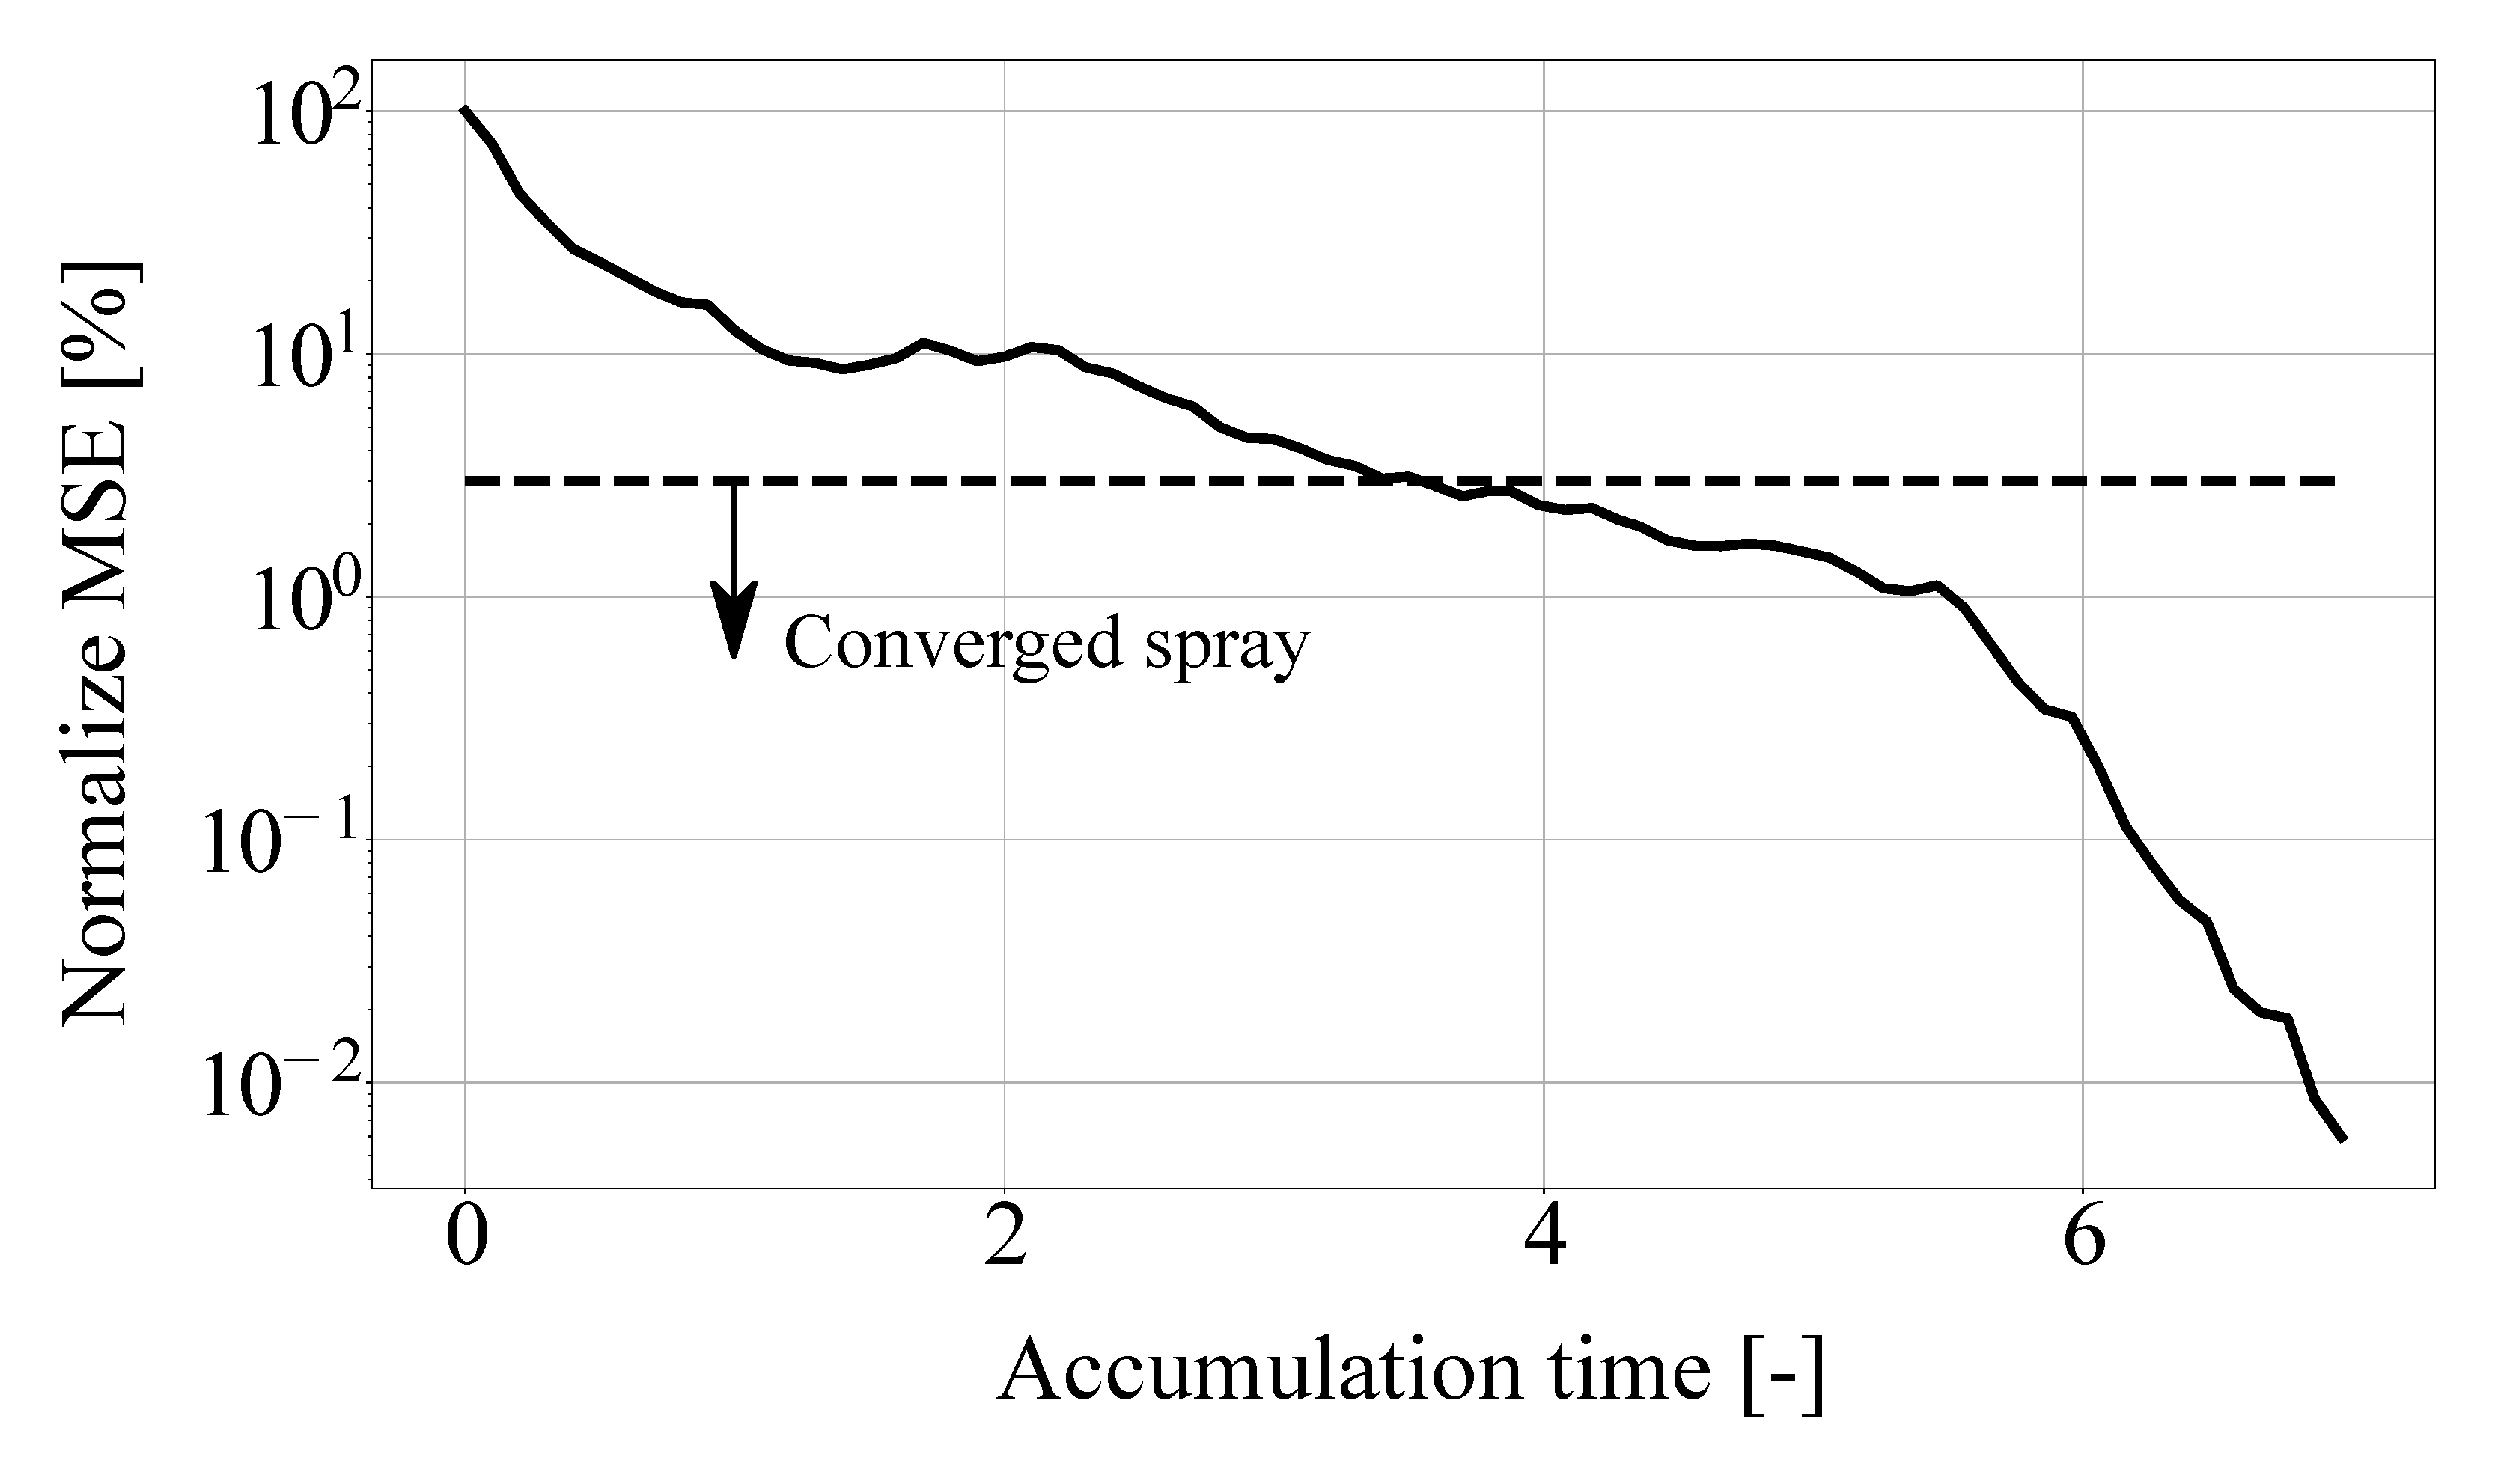
\includegraphics[scale=0.15]{./part2_developments/figures_ch4_SLI/spray_convergence_with_text.eps}
	\caption[Evolution of Normalized Mean Squared Error (NMSE) with respect to spray accumulation time.]{Evolution of Normalized Mean Squared Error (NMSE) with respect to spray accumulation time (solid line). The dashed line indicates the chosen threshold of $\varepsilon_\mathrm{th} = 3 \%$.}
	\label{fig:NMSE_evolution}
\end{figure}



It is worth noting that the convergence criterion based on NMSE introduced in this section depends solely on the equivalent droplets size $d_\mathrm{dr}$. Future work would include to extend this criterion to other magnitudes fundamental for a proper spray representation, such as velocities and flow rates. Furthermore, a time-independent spray has been considered in all the previous process by accumulating droplets and calculating statistics which do not depend on the time when they were sampled. A perspective in this respect would be to obtain a transient spray in order to create unsteady numerical injectors. This could be useful in systems where thermoacoustic instabilities appear and there are fluctuations in the injected flow rates, such as aeronautical gas turbines \citepColor[lieuwen_unsteady_2012]. Further possible improvements could also include the use of information theory techniques for characterizing the convergence state, which have recently been applied and evaluated in sprays \citemColor[panao_assessment_2012,panao_statistical_2020].


%\subsubsection*{Old formulation}
%
%
%A Mean Squared Error (MSE) function is used:
%
%\begin{equation}
%MSE = \frac{1}{n} \sum_{i=1}^n \left( P_{N_{\mathrm{dr},2}} - P_{N_{\mathrm{dr},1}} \right)^2
%\end{equation}

\subsection{Spatial discretization of sprays}
\label{subsec:SLI_spatial_discretization}

Once the global accumulated spray at the sampling plane is converged according to the NMSE criterion, enough droplets have been sampled to perform a spatial discretization of the spray. The objective is to classify spatially the in-plane accumulated droplets into a grid composed of several rectangular probes so that spray statistics can be calculated within each probe individually. Later on each probe will conform an injector for the dispersed-phase simulations: the SLI is therefore the whole grid composed of all the discrete injectors.

Figure \ref{fig:SLI_discretization} shows an example of a discrete spray grid resulting from the spatial discretization process. The grid has dimensions ($w_\mathrm{spray}$, $h_\mathrm{spray}$), which correspond to its width and height given in the $y$ and $z$ directions respectively. Grid's dimensions can be calculated in three ways: 1) they can be chosen ad-hoc by the user (as long as they englobe the full spray in order not to miss sampled mass); 2) they are calculated automatically as given by the furthest droplets in the $y$, $z$ directions; 3) they are calculated automatically if the individual probe dimensions ($w_\mathrm{inj}$, $h_\mathrm{inj}$) are given by the user, in which case the grid size will be calculated accordingly in order to englobe the whole in-plane spray. The sketch at the right in Figure \ref{fig:SLI_discretization} shows a magnified view of a single probe of the grid, which composes an individual injector. The probe consists of dimensions ($w_\mathrm{inj}$, $h_\mathrm{inj}$) and center $x_\mathrm{inj}$. Each droplet in the probe is characterized by the parameters from Table \ref{tab:sampling_parameters}, from which the equivalent droplet diameter $d_\mathrm{dr}$ is calculated with Eq. (\ref{eq:ch4_r_equivalent_calculation}) and the deformation parameters $\alpha$ and $\beta$ with Eq. (\ref{eq:ch4_deformation_parameters_alpha_beta_calculation}). These parameters are then used to calculate statistics on each probe's spray, which are later used to perform injection. The parameters conforming each injector are later introduced in $\S$\ref{subsec:ch4_injectors_definition}. The spatially distributed statistics in the sampling grid can be represented in maps of mean and RMS values, which give an idea of the spray shape in terms of diameters, fluxes and velocity distributions. Examples of maps for the resolved simulations of liquid JICF cases are shown later in Chapters \ref{ch5:jicf_resolved_simulations} ($\S$\ref{sec:ch5_learning_SLI}) and \ref{ch8:bimer_resolved_atomization} ($\S$\ref{sec:ch8_learning_SLI_in_BIMER}).

\clearpage

\begin{figure}[h!]	
	\centering
	\includeinkscape[inkscapelatex=false,width=10cm]{./part2_developments/figures_ch4_SLI/plane_injection_sketch}
	\caption{Schematic of a discrete grid composed of individual spray probes. The zoomed-in probes shows an example of droplets and parameters characterizing the probe and the spray within it that served as injectors.}
	\label{fig:SLI_discretization}
\end{figure}


\subsection{Convergence-driven discretization}
\label{subsec:SLI_quadtrees_discretization}

Among all parameters being calculated in each individual probe, the NMSE is also calculated in the same way as explained in $\S$\ref{subsec:SLI_spray_convergence}. Then, the local convergence level of each probe's spray is estimated, which gives an idea of the spatial convergence distribution in the SLI. This local convergence can be used to further refine the grid in those probes which present a converged spray, as shown in the flowchart of Figure \ref{fig:SLI_graphic_description}. Hereafter, the full spray will be referred as \textbf{global spray} and the discretized spray will be named \textbf{local spray}.

If convergence-driven discretization is performed, those probes presenting convergence will be further refined by a factor $\times 2$: i.e. the probe will be split into 4 probes of size ($w_\mathrm{inj}/2$, $h_\mathrm{inj}/2$). This will conform a refined grid with the same global dimensions ($w_\mathrm{spray}$, $h_\mathrm{spray}$) but containing more elements, and spray statistics will be calculated into each new probe for the spray contained within it. If the refined elements are again converged according to the NMSE criterion and further refinement is wished to be done, the process can be repeated again and as many times as desired. This discretization process, known as \textbf{quadtrees}, is therefore base in a tree structure with several levels of refinement, and has been widely used for performing Adaptive Mesh Refinement (AMR) in grids for solving two-phase resolved atomization problems \citemColor[popinet_gerris_2003, fuster_simulation_2009, zuzio_direct_2010]. Figure \ref{fig:quadtrees_tree_structure} shows an example of quadtrees refinement in a 2x2 SLI with two refinement levels (left) and the resulting SLI (right).



\begin{figure}[h!]	
	\centering
	\includeinkscape[inkscapelatex=false,scale=0.8]{./part2_developments/figures_ch4_SLI/quadtrees_tree_structure}
	\caption[Convergence-driven discretization of SLI according to a quadtrees structure.]{Convergence-driven discretization of SLI according to a quadtrees structure. \textsl{Left}: quadtree structure with two tree levels, where the converged elements refined are shadowed. \textsl{Right}: resulting discretized injector. }
	\label{fig:quadtrees_tree_structure}
\end{figure}


%\subsubsection{Numerical implementation}
%
%The numerical implementation of the process works as follows:
%
%\begin{enumerate}
%
%	\item From global spray, create a 3x3 grid (\textbf{parent grid}).
%	
%	\item From global spray, create a 6x6 grid (\textbf{children grid}).
%	
%	\item Map children elements to parent elements to check local convergence:
%	
%	\begin{enumerate}
%	
%		\item If all children elements belonging to parent element are converged, \textbf{refine}: keep statistics from 6X6 grid.
%		
%		\item If not all children elements are converged, then \textbf{unrefine}: store parent elements characteristics into grid (mean and RMS velocities, SMD, volume flux),  and divide flux by 4.
%	
%	\end{enumerate}
%
%\end{enumerate}



\subsection{Injectors definition}
\label{subsec:ch4_injectors_definition}

Once a spatially-discretized injector is obtained (either if convergence-driven discretization has been applied or not), an SLI is built. An example of an injectors and the accumulated droplets within it was shown in Figure \ref{fig:SLI_discretization}. Each injector has then the following characteristics in terms of topology and spray characteristics calculated:

\begin{itemize}

	\item \textbf{Injector topology} defined by its width $w_\mathrm{inj}$, height $h_\mathrm{inj}$ and center $\textbf{x}_\mathrm{inj}$. From the injector dimensions, its injection surface (called probe surface) is calculated as $S_\mathrm{probe} = w_\mathrm{inj} \times h_\mathrm{inj}$. All these parameters are calculated after the spatial discretization process. A lagrangian particle will be injected at a point $x_i$ randomly located within the injection surface: the number of injection points $N_\mathrm{pts}$ in each probe needs to be specified by the user. Results from dispersed phase simulations have shown not to be sensitive to this value, so if not specified it is set by default to 5.
	
	\item \textbf{Flow rate} $Q_l$ to be delivered through the injector. This value is calculated with applying Eq. (\ref{eq:ch4_Ql_definition}) to each individual probe. $Q_l$ determines the number of droplets to be injected at each time step. If divided by the probe surface $S_\mathrm{probe}$, the volume flux $q_l$ is obtained as given by Eq. (\ref{eq:ch4_Ql_definition}). Nevertheless, this quantity is useful for graphical visualization of the spray with volume flux maps but cannot be specified to perform injection: the absolute flux $Q_l$ needs to be supplied instead.
	
	\item \textbf{Droplets diameters distribution} $f_0 \left( d \right)$. Since all the information on (equivalent) droplets size sampled and accumulated from resolved atomization simulations are available, the diameter of the injected droplets can be specified to the injector. Three options are possible for the distribution $f_0$: 1) to provide directly the sampled size histogram from the resolved simulations; 2) provide a size PDF that fits the histogram, such as a lognormal or Rosin-Rammler distribution \citepColor[lefebvre_atomization_2017]; 3) provide a constant diameter to all the droplets. Each lagrangian droplet injected $d_i$ is therefore either sampled from $f_0$ when the desired injection size is done according to a histogram of PDF, or constantly set as $d_i = \mathrm{SMD}$ where SMD is calculated with Eq. (\ref{eq:ch4_SMD_definition}).
	
	\item \textbf{Spray velocities}. As with particle diameters, the velocity components of each sampled and accumulated droplet from resolved atomization simulations is available. These velocities can be treated statistically in order to obtain reliable velocity injection values for the dispersed-phase simulations. However, on the contrary to the injectors, here no velocity distributions are used but instead the mean and RMS velocities are calculated by plugging $f = u$ into Eqs. (\ref{eq:ch4_f_arbitrary_mean_RMS_definition}) and (\ref{eq:ch4_f_arbitrary_mean_RMS_VW_definition}) to yield arithmetic and volume-weighted mean and RMS velocities, respectively. Then, injection of a lagrangian particle $i$ is performed according to the following law:
	
%	\begin{equation}	\label{eq:ch4_lagrangian_injection_velocity_with_mean_and_rms}
%	\boldsymbol{u}_\mathrm{i} = \overline{\boldsymbol{u}} + \boldsymbol{r}^T \boldsymbol{u}_\mathrm{RMS}
%	\end{equation}
	
	\begin{equation}	\label{eq:ch4_lagrangian_injection_velocity_with_mean_and_rms}
	\boldsymbol{u}_\mathrm{i} = \overline{\boldsymbol{u}} + r \boldsymbol{u}_\mathrm{RMS}
	\end{equation}
	
	where $\overline{\boldsymbol{u}}$ is the mean velocity and $\boldsymbol{u}_\mathrm{RMS}$ is the RMS one. If volume-weighted velocities are injected, the calculated parameters $\overline{\boldsymbol{u}}_\mathrm{VW}$ and $\boldsymbol{u}_\mathrm{RMS,VW}$ are used instead. The parameter $r$ is a random number that multiplies the RMS to provide a varying velocity through all the injection process. Three different laws are available to sample random numbers for $r$, being these ones:
	
	\begin{itemize}
	
	\item \textbf{Uniform law}. $r$ follows a uniform distribution: $r \sim \mathcal{U} \left(-\sqrt{3},  \sqrt{3} \right)$, where $-\sqrt{3}$ and $\sqrt{3}$ are the limits of the distribution. Such values are set so that the RMS of the signal from Eq. (\ref{eq:ch4_lagrangian_injection_velocity_with_mean_and_rms}) maintains its RMS provided values.
	
	\item \textbf{Gaussian law}. $r$ follows a normal distribution $r \sim \mathcal{N} \left( \mu = 0, \sigma^2 = 1 \right)$, where $\mu$ is the mean and $\sigma^2$ the variance. Such values are set so that the RMS of the signal from Eq. (\ref{eq:ch4_lagrangian_injection_velocity_with_mean_and_rms}) maintains its RMS provided values.
	
	\item \textbf{Zero law}. In this case the RMS are not considered for injection and only constant velocities equal to mean resolved velocities are injected, therefore $r = \textbf{0}$.
	
	\end{itemize}

\end{itemize}

Apart from the spray parameters to perform injection, the following liquid physical properties also need to be specified: density $\rho_l$, viscosity $\mu_l$ and surface tension $\sigma$. The density is needed in the dispersed-phase simulations to calculate the dynamics of the droplets according to Eqs. (\ref{eq:TPF_lagrange_dynamic_eqs}), while the viscosity and surface tension are used by the secondary atomization models to estimate the breakup time and children radii of lagrangian droplets ($\S$\ref{sec:ch4_secondary_atomization_modeling}). A summary of all the parameters involved in SLI and the way in which they are calculated is provided in Table \ref{tab:ch4_sli_injection_parameters_master_slide}.




\begin{table}[ht]
\centering
\caption{Summary of SLI injection parameters}
\begin{tabular}{cccc}
\thickhline
\textbf{Group} & \textbf{Parameter} & \textbf{Description} &\textbf{Obtention method} \\
\thickhline 
\multirow{9}{*}{ \begin{tabular}{c} \textbf{Injector} \\ \textbf{topology} \end{tabular}} & \multirow{2}{*}{$\textbf{x}_\mathrm{inj}$} & \multirow{2}{*}{Injector center} & Calculated through \\
& & & discretization process \tab_space
%\cline{2-4}
 & \multirow{2}{*}{$w_\mathrm{inj}$} & \multirow{2}{*}{Injector width} & Calculated through \\
& & & discretization process \tab_space 
%\cline{2-4}
 & \multirow{2}{*}{$h_\mathrm{inj}$}  & \multirow{2}{*}{Injector height} & Calculated through \\
 & & & discretization process \tab_space
%\cline{2-4}
& \multirow{2}{*}{$N_\mathrm{pts}$} & Number of injection  & \multirow{2}{*}{User-defined} \\
& & points in the injector & \tab_space
\thickhline

\multirow{17}{*}{ \begin{tabular}{c} \textbf{Spray} \\ \textbf{characteristics} \end{tabular}} & \multirow{2}{*}{$Q_{l}$} & Absolute flux & \multirow{2}{*}{Eq. (\ref{eq:ch4_Ql_definition})}  \\
& &  to be injected & \tab_space
%\cline{2-4}
& \multirow{2}{*}{$f_{0}$} & Droplet size & Histogram, PDF fit   \\
& &  distribution & or constant (SMD) \tab_space
& \multirow{2}{*}{ $\overline{\textbf{u}}$ } & Arithmetic mean & Eq. (\ref{eq:ch4_f_arbitrary_mean_RMS_definition})  \\
& &  injection  velocities & with $f = \textbf{u}$ \tab_space
& \multirow{2}{*}{ $\textbf{u}_\mathrm{RMS}$ } & Arithmetic RMS & Eq. (\ref{eq:ch4_f_arbitrary_mean_RMS_definition}) \\
& & injection  velocities & with $f = \textbf{u}$ \tab_space
& \multirow{2}{*}{ $\overline{\textbf{u}}_\mathrm{VW}$ } & Volume-weighted mean & Eq. (\ref{eq:ch4_f_arbitrary_mean_RMS_VW_definition})   \\
& &  injection  velocities & with $f = \textbf{u}_\mathrm{VW}$ \tab_space
& \multirow{2}{*}{ $\textbf{u}_\mathrm{VW,RMS}$ } & Volume-weighted RMS & Eq. (\ref{eq:ch4_f_arbitrary_mean_RMS_VW_definition})  \\
& & injection  velocities & with $f = \textbf{u}_{\scriptsize  \mathrm{VW}}$\tab_space
& \multirow{2}{*}{ $r$ } & Random numbers law & \multirow{2}{*}{ User-defined  }\\
& &  to multiply $\textbf{u}_\mathrm{RMS}$ & \tab_space
\thickhline

\multirow{7}{*}{ \begin{tabular}{c} \textbf{Particle} \\ \textbf{properties} \end{tabular}}& \multirow{2}{*}{$\textbf{x}_\mathrm{i}$} & \multirow{2}{*}{Injection location} &  Randomly chosen from the  \\
& & & injection points \tab_space
%\cline{2-4}
& \multirow{2}{*}{$d_i$} & \multirow{2}{*}{Drop diameter} & Randomly sampled from $f_0$, \\ 
& & & or constant if SMD \tab_space
%\cline{2-4}
& $\textbf{u}_i$ & Drop injection velocity & Eq. (\ref{eq:ch4_lagrangian_injection_velocity_with_mean_and_rms}) \tab_space
%\cline{2-4}
% & $\textbf{u}_\mathrm{RMS}$ & Drop RMS velocity & User-defined \tab_space
% & $\textbf{r}$ & Factor for RMS & User-defined \tab_space

\thickhline
\multirow{4}{*}{ \begin{tabular}{c} \textbf{Liquid} \\ \textbf{properties} \end{tabular}} & $\rho_l$ & Particle's density & User-defined \tab_space
%\cline{2-4}
 & $\mu_l$ & Particle's viscosity & User-defined \tab_space
%\cline{2-4} 
& $\sigma$ & Surface tension & User-defined \\
\thickhline
\end{tabular}
\label{tab:ch4_sli_injection_parameters_master_slide}
\end{table}

\clearpage


\section{Dense core blockage effect modeling}
	\label{sec:ch4_dense_core_modelling}
	
One of the biggest advantages of resolved atomization simulations is the resolution of the liquid-gas interaction. This allows capturing the perturbation effect from the liquid jet to the gaseous phase, which creates turbulent structures that affect droplets dispersion. In the jet in crossflow this influence is paramount, since the liquid coherent structures impose a blockage effect to the gaseous phase that creates vortices downstream the liquid injection nozzle (see Figure \ref{fig:arienti_2006_jicf} and Chapter \ref{ch5:jicf_resolved_simulations}) % $\S$\ref{subsec:ch5_dense_core_in_ACLS_simus}).

Perturbation effects are not taken into account \textsl{a priori} in dispersed phase simulations, since the coherent structures are not present. As illustrated in $\S$\ref{sec:ch3_state_art_lagrangian_injection}, some approaches have succeeded in emulating this interaction between phases by injecting lagrangian big droplets according to the the blob method \citepColor[reitz_modeling_1987] and adding a two-way coupling between liquid and gaseous phases \citemColor[apte_les_2003,senoner_simulation_2010]. Other studies have solved and kept the liquid coherent structures with VOF to capture the interaction, and then performed lagrangian injection and spray transport \citemColor[arienti_aerodynamic_2006,fontes_improved_2019].

In this work, the blockage effect is modeled in dispersed phase computations by means of the Actuator Line Method (ALM). This method has been, to the author's knowledge, only used up to date in wind turbine simulations for modeling the turbulent wakes created by the tower and blades. Firstly, a review on the theory and some previous works in ALM is done. Secondly, a simple model for representing the dense core with ALM is proposed. This model will be later fed from the resolved atomization simulations of Chapter \ref{ch5:jicf_resolved_simulations} and applied to dispersed phase computations in Chapter \ref{ch6:jicf_lgs_simulations}.


\subsection{Actuator Line Method}

A proper modeling of wind turbines and windfarms requires an accurate representation of the wakes generated by the presence and movement of the blades. Since performing DNS is unaffordable due to the wide range of space and time scales found in these problems, LES are often used. For a proper representation of the wakes in these computations, aerodynamic models are added to consider the effect of the moving blades. The first developed model in this research line was the Actuator Disk Method (ADM) \citepColor[sorensen_unsteady_1992]. The moving blades are modeled as a disk which interacts with the incoming air. This perturbation is taken into account by means of body forces in the Navier-Stokes equations that influence the gaseous flow field. The purpose of ADM is the determination and imposition of these forces.

An extension of the ADM was done later by \citeColor[sorensen_numerical_2002], known as \textbf{Actuator Line Method} (ALM). In this case, the moving bodies are not represented by a disk but by lines emulating the rotor blades. Each individual blade is discretized by points which are equally spaced by a length $w$. A body force is imposed in each blade point. The cross section of a blade has an airfoil shape (see Figure \ref{fig:ALM_airfoil_and_mollification_benard} left), so the forces imposed by ALM to the flow field can be calculated from Blade Element Momentum (BEM) theory \citepColor[hansen_aerodynamics_2015]:

\begin{subequations}
\label{eq:ALM_lift_drag_definitions}
\begin{align}
L &= \frac{1}{2} \rho_g u_\mathrm{rel}^2 c \left( r \right) w C_L \left( r \right) \\
D &= \frac{1}{2} \rho_g u_\mathrm{rel}^2 c \left( r \right) w C_D \left( r \right)
\end{align}
\end{subequations}

where $L$ is lift, $D$ is drag, $u_\mathrm{rel}$ the relative velocity, $c \left( r \right)$ the chord size at the span direction $r$, and $C_L \left( r \right)$ and $C_D \left( r \right)$ lift and drag coefficients respectively. With this methodology, the variation of the forces along the span direction can be taken into account through changing chord and coefficients. The chord is given by the blade geometry, while the lift and drag coefficients are tabulated for each airfoil.


\begin{figure}[h!]
	\centering
	\includegraphics[scale=0.4]{./part2_developments/figures_ch4_SLI/ALM_airfoil_and_mollification_benard}
	\caption[ALM illustration of a velocity triangle and geometrical conventions in an airfoil and mollification of a point force on several nodes of an unstructured grid]{ALM illustration of a velocity triangle and geometrical conventions in an airfoil (\textsl{left}) and mollification of a point force on several nodes of an unstructured grid (\textsl{right}). Source: \citeColor[benard_large-eddy_2018].}
	\label{fig:ALM_airfoil_and_mollification_benard}
\end{figure} 
 

In the computational domain, the body forces cannot be directly applied in a single point since it would create a numerical singularity in the Navier-Stokes equations. Therefore, the body source term is applied using a mollifying function $\eta$ that distributes the body force $f$ from the forces calculated at each blade element:

\begin{equation}
\textbf{f} \left( \textbf{x}, t \right) = - \sum_{e=1}^{N} \left( L \textbf{e}_L + D \textbf{e}_D \right) \eta \left( |\textbf{r} - \textbf{r}_e| \right)
\end{equation}

where $\textbf{e}_L$ and $\textbf{e}_D$ are the unit vectors along the lift and drag directions (Figure \ref{fig:ALM_airfoil_and_mollification_benard} left), the subscript $e$ refers to each blade element and the mollifying function is defined by Eq. (\ref{eq:ch4_ALM_mollification_function}).

\begin{equation}
\label{eq:ch4_ALM_mollification_function}
\eta \left( d \right) = \frac{1}{\epsilon^3 \pi^{3/2}} \exp \left[ - \left( \frac{d}{\epsilon} \right)^2 \right]
\end{equation}

where $\epsilon = 2 w$. The mollification process is depicted in Figure \ref{fig:ALM_airfoil_and_mollification_benard} right. The simplicity of ALM and its applicability to represent the perturbations created by solid blades have seen its application to model the interaction with other bodies, such as towers in wind turbines \citeColor[benard_large-eddy_2018], and to use it for generating synthetic turbulence in the grids \citepColor[houtin-mongrolle_actuator_2020]).

%As shown in Figure (\textbf{Ref. to figure in introduction}), the dense core has a perturbation effect towards the gas phase. The resulting vortical structures will influence the dispersion of the droplets generated by atomization due to turbulent interaction. Therefore,


\subsection{Dense core representation as an actuator}

%In this work, ALM is used to model the perturbation effect of the JICF dense core on the gaseous field in dispersed phase simulations. 

As depicted in Figure \ref{fig:arienti_2006_jicf}, the presence of the dense core creates a wake and vortical structures further downstream. This interaction can be captured in resolved atomization simulations (see $\S$\ref{subsec:ch5_dense_core_in_ACLS_simus} of Chapter \ref{ch5:jicf_resolved_simulations}), but not in dispersed phase simulations where the coherent liquid structures are neglected. Since these liquid-gas interactions can have a strong influence on the transport of droplets in the developed spray region, it is of interest to model this effect in dispersed phase simulations. For this purpose, ALM is used.

\begin{figure}[h!]	
	\centering
	\includeinkscape[inkscapelatex=false,width=13cm]{./part2_developments/figures_ch4_SLI/ALM_DC_learning}
	\caption[Representation of the dense core as an actuator]{Representation of the dense core as an actuator, showing lateral (\textsl{left}) and frontal (\textsl{right}) views of the jets. \textsl{Top}: schematic dense core from a resolved simulation. \textsl{Bottom}: actuator line model of the dense core.}
	\label{fig:ALM_DC_learning}
\end{figure}

Figure \ref{fig:ALM_DC_learning} shows the representation of the dense core (top figures) as an actuator line model (bottom figures). Its complex topology is emulated by a frustum with increasing chord from the bottom ($c_0 = d_\mathrm{inj}$) to the top ($c_L = W$). The frustum has a length $L$ and an inclination angle $\theta$ which are obtained from the breakup point coordinates $(x_b, z_b)$ of the dense core in resolved atomization simulations: $L = \sqrt{x_b^2 + z_b^2}$ and $\theta = \tan^{-1} \left( z_b / x_b\right)$. The actuator points where discrete forces are placed are equally-spaced with a distance $w$ along the center line of the frustum. The number of points $N_p$ also needs to be specified in the ALM model.

Apart from the geometry, the forces applied to the actuator points are also defined. In this model, instead of specifying coefficients as done in wind turbine blades, the forces will be directly imposed in the actuator points. As shown in Figure \ref{fig:ALM_DC_learning}c, the force in the actuator will evolve linearly from the bottom to the top in order to take into account the real increasing cross-section of the actuator, which has the effect of increasing drag \citepColor[mashayek_jet_2006]. The force acts in a direction normal to the axis of the frustum. Therefore, the imposed forces can be decomposed into two components: a drag force $D$ along the $x$ direction and a lift force $L$ along the $z$ direction. Forces are specified at each actuator point with coordinates $\left( x_p, z_p \right)$ along the actuator. As the coordinates are automatically calculated according to the number of actuator points $N_p$ and the breakup point $\left( x_b, z_b \right)$, the forces will be expressed with respect to the line coordinate $s_p = \left( x_p^2 + z_p^2 \right)^{1/2}$ with expresses the distance of each actuator point to its base. Hence, the force decomposition into lift and drag holds as follows:

\begin{equation}
\textbf{F} \left( s_p \right) = D \left( s_p \right) \textbf{i} + L \left( s_p \right) \textbf{k} 
\end{equation}

where $\textbf{i}$ and $\textbf{k}$ are the unit vectors in the $x$ and $z$ directions, respectively. To estimate these forces, the net force applied to the dense core $\textbf{F}_\mathrm{DC}$ is obtained from the resolved simulations (see $\S$\ref{subsec:ch4_ALM_forces_determination}). This force is assumed to act in the same direction as the forces $\textbf{F} \left( s_p \right)$ from the actuator model, and is repartitioned into the several forces that are applied to the actuator points. Therefore, the following condition must be fulfilled:

\begin{equation}
\sum_{p=1}^{N_p} | \textbf{F} \left( s_p \right)| = | \textbf{F}_\mathrm{DC} |
\end{equation}

As the forces $| \textbf{F} \left( s_p \right)|$ increase linearly along the actuator, its evolution is represented by the following expression accordingly to the vertical coordinates $z_p$ of the actuator points:

\begin{equation}
|\textbf{F} \left( s_p \right) | = | \textbf{F}_\mathrm{DC} | \frac{s_p}{\sum_{p=1}^{N_p} s_p}
\end{equation}

And finally, the drag and lift forces to impose are calculated as follows:

\begin{subequations}
\label{eq:ALM_SLI_lift_drag_definitions}
\begin{align}
L \left( s_p \right) &= - |\textbf{F} \left( s_p \right) | \cos \theta = - | \textbf{F}_\mathrm{DC} | \cos \theta \frac{s_p}{\sum_{p=1}^{N_p} s_p} \\
D \left( s_p \right) &= |\textbf{F} \left( s_p \right) | \sin \theta = | \textbf{F}_\mathrm{DC} | \sin \theta \frac{s_p}{\sum_{p=1}^{N_p} s_p}
\end{align}
\end{subequations}

Therefore, the forces imposed to the actuator points are parametrized by the dense core net force $| \textbf{F}_\mathrm{DC} |$, the actuator inclination $\theta$ and the actuator points. Table \ref{tab:alm_parameters} shows a recap of the parameters used in the proposed model. In this table, the angle $\theta$ is not shown since it can be obtained with trigonometry from the initial and end points of the actuator. The number of actuator points $N_p$ is not taken as an input parameter as it has been checked that, if large enough, it does not have an effect of the perturbed flow field: therefore, it has been set to $N_p = 100$ for all cases presented in this thesis.

%The actuator chords shown in Figure \ref{fig:ALM_DC_learning} are not shown in this model since the increase in cross-section is directly contained in the linear evolution of the forces, Eqs. (\ref{eq:ALM_lift_drag_definitions}).

\begin{table}[!h]
\centering
\caption{Parameters of an actuator representing the dense core}
\begin{tabular}{ccc}
\thickhline
\textbf{Parameter} & \textbf{Units} & \textbf{Description} \\ 
\thickhline
$x_b, z_b$ & mm & Actuator end point  \\
%$c_0$ & mm & Chord at base of actuator \\
%$c_L$ & mm & Chord at tip of actuator \\
%$\theta$ & $\degree$ & Dense core inclination  \\
$| \textbf{F}_\mathrm{DC} |$ & N & Dense core net force\\
%$\Delta p$ & Pa & \\
\thickhline 
\end{tabular}
\label{tab:alm_parameters}
\end{table}


\subsection{Determination of forces}
\label{subsec:ch4_ALM_forces_determination}

The forces to impose in the actuator model are learnt from the resolved atomization simulation. For this purpose, they are firstly calculated in these simulations by calculating the corresponding term of the momentum equation (\ref{eq:momentum_conservation_general_integral}):

\begin{equation}
\boldsymbol{F}_\mathrm{DC} = \boldsymbol{F}_p + \boldsymbol{F}_\tau = \int_{\partial \Omega_{DC}} \left( \underbrace{- p \boldsymbol{n}}_{\mathrm{Pressure}} + \underbrace{2 \mu \overline{\overline{\epsilon}} \boldsymbol{n}}_{\mathrm{Shear}}  \right) dS 
\end{equation}

where $\partial \Omega_{DC}$ denotes the dense core surface. $\boldsymbol{F} $ has two contributions: a pressure force term and a shear force term. In a first instance, the shear term is neglected (see next section for details). Therefore, the total force term is reduced to the pressure force:

\begin{equation}
\label{eq:ALM_Fp_complete_integral}
\boldsymbol{F}_\mathrm{DC} = \boldsymbol{F}_p = - \int_{\partial \Omega_{DC}} p \boldsymbol{n} dS 
\end{equation}

To simplify this expression, the forces in the windward and leeward sides of the dense core are assumed to be constant as indicated in Figure \ref{fig:ALM_DC_learning}a by the red and blue arrows, respectively. The surface of the dense core can be approximated according to the actuator model as $\partial \Omega_\mathrm{DC} \approx S_\mathrm{DC} = \frac{1}{2} \left( c_0 + c_L \right) L$, being $L = \sqrt{x_\mathrm{b}^2+z_\mathrm{b}^2}$ if the actuator initial point is located at the origin of the coordinate system. Therefore, Eq. (\ref{eq:ALM_Fp_complete_integral}) can be reduced to


\begin{equation}
\label{eq:ALM_Fp_calculation_simplified}
\boxed{
|\boldsymbol{F}_\mathrm{DC}| = \left( p_\mathrm{windward} - p_\mathrm{leeward} \right) S_{DC} 
}
\end{equation}


%The approximation of considering the pressures as both sides as equal is done in this model as it has been observed in the resolved simulations (see Figure \textbf{????}), but requires further research and might be a source of error. 

It must be taken into account that the dense core as a rigid body immersed in a fluid. Its geometry has been approximated by observations of the dense core shape in resolved atomization simulations, and have been taken as constant. In reality, the dense core is a deformable body whose topology (breakup point, inclination, length) changes with time. Future works on deriving more thorough models intending to represent the dense core should take into account these transient properties \citepColor[patil_liquid_2021].

\subsubsection*{Neglecting the shear force term}

For a body immersed in a fluid, the shear force is defined as:

\begin{equation}
\boldsymbol{F}_\tau = \int_{\partial \Omega_\mathrm{DC}} 2 \mu \overline{\overline{\epsilon}} \boldsymbol{n} dS
\end{equation}

where $\overline{\overline{\epsilon}}$ is the deformation tensor:

\begin{equation}
\overline{\overline{\epsilon}} = \frac{1}{2} \left( \nabla \boldsymbol{u} + \left(\nabla \boldsymbol{u}\right)^T \right)
\end{equation}

The forces $\boldsymbol{F}_\tau$ cannot be easily calculated with the current methodology. Instead, a more simple expression of the shear forces based on a friction coefficient $C_f$ and a reference surface $S$ is used \citemColor[johnston_investigation_1984,soedarmo_simplified_2018]:

\begin{equation}
\label{eq:ALM_model_Ftau}
\boldsymbol{F}_\tau = \frac{1}{2} \rho_g u_g^2 S C_f 
\end{equation}

The friction coefficient $C_f$ is obtained from the following expression \citepColor[yang_new_2017]:

\begin{equation}
\label{eq:ALM_model_Cf}
C_f = 0.37 \left( \log Re_x \right)^{-2.584}
\end{equation}

where $Re_x$ is the Reynolds number based on the incoming velocity and the distance along the dense core.

The relative intensity of the force $\boldsymbol{F}_p$ with respect to $\boldsymbol{F}_\tau$ can be measured by dividing expressions (\ref{eq:ALM_Fp_calculation_simplified}) and (\ref{eq:ALM_model_Ftau}), plugging also Eq. (\ref{eq:ALM_model_Cf}):

\begin{equation}
\label{eq:rF_definition}
r_F = \frac{| \boldsymbol{F}_p| }{| \boldsymbol{F}_\tau |} = \frac{\Delta p}{0.185 \rho_g u_g^2 \left( \log Re_x \right)^{-2.584}}
\end{equation}

\paragraph*{Numerical application to JICF operating conditions}

The force ratio from Eq. (\ref{eq:rF_definition}) can be estimated for the operating conditions of interest in this thesis. These correspond to the high-pressure jet in crossflow simulated in Chapter \ref{ch5:jicf_resolved_simulations}. The pressure diference for these cases is $\Delta p \sim O \left( 10^4 \right)$ (see Table \ref{tab:dense_core_geometry_pressures_and_force_parameters} for specific values). Considering this value, the expression for $r_F$ can be estimated to be:

\begin{equation}
r_F \sim \frac{10^5}{\rho_g u_g^2 \left( \log Re_x \right)^{-2.584}}
\end{equation}

In the operating points studied (summarized in Table \ref{tab:jicf_operating_conditions}), $\rho_g = 7.21$ kg m$^{-3}$ and $u_g = 75; 100$ m s$^{-1}$. Then, $Re_x$ ranges from $10^3$ to $10^5$. With these values, $r_F$ is plotted as a function of $Re_x$ in Figure \ref{fig:ALM_rF_vs_Rex}. As observed, the ratio $r_F$ presents values between 10 to 90 for the $Re_x$ range of interest. These ratios mean that the pressure force $\boldsymbol{F}_p$ is between 10 and 90 times the shear force $\boldsymbol{F}_\tau$. Therefore, $|\boldsymbol{F}_\tau| << |\boldsymbol{F}_p|$ and only the contribution of the pressure force is considered to calculate the dense core net force.




\begin{figure}[h!]
	\centering
	\includegraphics[scale=0.5]{./part2_developments/figures_ch4_SLI/ALM_rF_vs_Rex.eps}
	\caption{Force ratio evolution with $Re_x$.}
	\label{fig:ALM_rF_vs_Rex}
\end{figure}



\section{Secondary atomization modeling}
\label{sec:ch4_secondary_atomization_modeling}

In disperse phase simulations, spray is modeled by a set of spherical and rigid particles whose dynamics are governed by the point-particle equations described in $\S$\ref{sec:ch3_EL_formalisms}. Due to these assumptions, particles will not break by their interaction with the gaseous phase as in the resolved atomization simulations. Nevertheless, further breakup can be taken into account by means of secondary atomization models. The most important parameter governing secondary atomization is the Weber number based on the relative velocities between liquid and gas $u_\mathrm{rel}$:

\begin{equation}
\label{eq:We_secondary_atomization_definition}
We = \frac{\rho_g u_\mathrm{rel}^2 r}{\sigma} 
\end{equation}

Different mechanisms produce secondary atomization depending on the value of We, see Fig. \ref{fig:regimes_atomization_secondary}. Existing models for secondary atomization have been developed for each particular mode of breakup, such as the WAVE model for high Weber numbers \citepColor[reitz_modeling_1987] or the Taylor Analogy Breakup (TAB) model for low ones \citepColor[orourke_tab_1987]. The former model predicts breakup by following a linear stability analysis considering Kelvin-Helmholtz waves as the governing breakup mechanisms, while the latter makes an analogy between a droplet and a second-order mechanical system. Nevertheless, up to date there is not a model which accounts for all different breakup mechanisms and that can capture all the physical complexity of secondary atomization.

In this work, three atomization models have been implemented and tested: the TAB model, the Enhanced TAB model \citepColor[tanner_liquid_1997], and the stochastic model of \citeColor[gorokhovski_stochastic_2001]. They are described in the following sections.

\subsection{Taylor Analogy Breakup}


\begin{figure}[h!]
	\centering
	\includeinkscape[inkscapelatex=false,scale=0.75]{./part2_developments/figures_ch4_SLI/TAB_analogy}
	\caption{Taylor analogy breakup between a droplet and a mechanical system with spring and damper. The undeformed droplet is represented by the dashed line, while the thick solid line depicts the droplet after deformation. $x$ is the displacement from the deformed to the undeformed states.}
	\label{fig:TAB_droplet_deformation}
\end{figure}

The Taylor Analogy Breakup (TAB) model is one the first secondary atomization models. Developed by \citeColor[orourke_tab_1987], it makes an analogy between a droplet and a mechanical system as shown in Fig. \ref{fig:TAB_droplet_deformation}. Breakup occurrence is estimated by solving the ordinary differential equation (ODE) representing the oscillating dynamics of the mechanical system depicted:

\begin{equation}
\label{eq:TAB_ODE_x}
m \ddot{x} = F - k x - c \dot{x}
\end{equation}

where $x$ is the displacement from the droplet's equator due to deformation, $m$ is the mass, $F$ is the external force, $k$ is the spring constant and $c$ is the damping coefficient. The Taylor analogy makes a comparison between this mechanical system and the droplet, producing the following relation between constants:

\begin{equation}
\frac{F}{m} = C_F \frac{\rho_g u_\mathrm{rel}^2}{\rho_l r} ~~~~ ; ~~~~ \frac{k}{m} = C_k \frac{\sigma}{\rho_l r^3} ~~~~ ; ~~~~ \frac{c}{m} = C_d \frac{\mu_l}{\mu_g r^2}
\end{equation}

where $C_F = 1/3$, $C_k = 8$, $C_d = 5$ are constants, $r$ the droplet radius, $\rho$ the density, $\sigma$ the surface tension, $\mu$ the viscosity, and the subscripts $l$ and $g$ indicate liquid and gases respectively. 

The deformation $x$ can be expressed by a non-dimensionless parameter $y$, hereafter referred as droplet distorsion, whose equivalence is $y = x / \left( C_b r \right)$, where $C_b = 0.5$ is a constant. Using the expressions from the Taylor analogy and introducing the change of variable $y$, the ODE (\ref{eq:TAB_ODE_x}) becomes:

\begin{equation}
\label{eq:TAB_ODE}
\ddot{y} = \frac{C_F}{C_b} \frac{\rho_g}{\rho_l} \frac{u_{rel}^2}{r^2} - \frac{C_k \sigma}{\rho_l r^3} y - \frac{C_d \mu_l}{\rho_l r^2} \dot{y}
\end{equation}

This expression governs the breakup of droplets, which occurs for $y > 1$ (i.e. when the amplitude of the oscillation $x$ equals the radius of the undeformed droplet). For solving this equation, it is useful to introduce the following parameters:

\begin{subequations}
\label{eq:TAB_td_omega_definition}
\begin{align}
t_d &= \frac{2 \rho_l r^2}{C_d \mu_l} \\
\omega^2 &= C_k \frac{\sigma}{\rho_l r^3} - \frac{1}{t_d^2}
\end{align}
\end{subequations}

where $t_d$ is the oscillation damping time and $\omega$ is the oscillations frequency. With these definitions, the solution to Eq. (\ref{eq:TAB_ODE}) is:

\begin{equation}
\label{eq:yTAB_equation_general}
y \left( t \right) = We_c + e^{- t / t_d} \left[ \left( y_0 - We_c \right) \cos \left( \omega t \right) + \frac{1}{\omega}\left( \dot{y}_0 + \frac{y_0 - We_c}{t_d} \right) \sin \left( \omega t \right)   \right]
\end{equation}

where $We_c = \frac{C_F}{C_k C_b} We = We / 12$ with the constants previously defined. The distorsion rate can be obtained by differentiating the former expression with time:

\begin{equation}
\label{eq:dydtTAB_equation_general}
\dot{y} \left( t \right) = \frac{We_c - y \left( t \right) }{t_d} + e^{- t / t_d} \left[ \left( \dot{y}_0 + \frac{y_0 - We_c}{t_d} \right) \cos \left( \omega t \right) - \omega \left( y_0 - We_c \right) \sin \left( \omega t \right)  \right]
\end{equation}

As it can be seen, the previous equations are continuous. For numerical implementation of the algorithm, it is more convenient to express them in their corresponding discrete form:

\begin{equation}
\label{eq:yTAB_equation_discrete}
y^{n+1} = We_c + e^{- dt / t_d} \left[ \left( y^n - We_c \right) \cos \left( \omega dt \right) + \frac{1}{\omega}\left( \dot{y}^n + \frac{y^n - We_c}{t_d} \right) \sin \left( \omega dt \right)   \right]
\end{equation}

\begin{equation}
\label{eq:dydtTAB_equation_discrete}
\dot{y}^{n+1} = \frac{We_c - y^{n+1} }{t_d} + e^{- dt / t_d} \left[ \left( \dot{y}^n + \frac{y^n - We_c}{t_d} \right) \cos \left( \omega dt \right) - \omega \left( y^n - We_c \right) \sin \left( \omega dt \right)  \right]
\end{equation}

where the subindexes $n$ and $n+1$ indicate two consecutive time instants separated by the timestep $dt$.

To estimate breakup, firstly $\omega^2$ is calculated with Eq. (\ref{eq:TAB_td_omega_definition}b). According to its value, two scenarios are possible:

\begin{itemize}

	\item If $\omega^2 < 0$, oscillations are not present. Hence, the droplet does not deform and the values for droplets distorsion and distorsion rate are set to $0$: $y^{n+1} = y^n = 0$.
	
	\item If $\omega^2 > 0$, breakup is possible. In this case, the amplitude of oscillations $A$ is calculated:
	
	\begin{equation}
	A = \sqrt{\left( y^n - We_c \right)^2 + \left( \dot{y}^n / \omega \right)^2}
	\end{equation}

\end{itemize}

Again, the value of $A$ will present two different alternatives:

\begin{itemize}

	\item If $We_c + A \leq 1$, then $y^n \leq 1$ and droplet will not break. Deformation and deformation rate will then be updated by applying Eqs. (\ref{eq:yTAB_equation_discrete}) and (\ref{eq:dydtTAB_equation_discrete}).
	
	\item If $We_c + A > 1$, breakup is possible. A breakup timestep $dt_{bu}$ is then calculated as the smallest root of the following equation:
	
	\begin{equation}
	\label{eq:TAB_dtbu_obtention}
	We_c + A \cos \left( \omega dt_{bu} + \phi  \right) = 1
	\end{equation}

\end{itemize}

where the phase $\phi$ is obtained from the following:

\begin{equation}
\cos \phi = \frac{\dot{y}^n - We_c}{A} ~~~~ ; ~~~~ \sin \phi = - \frac{\dot{y}^n}{A \omega}
\end{equation}

Breakup will then occur for $dt < dt_{bu}$, or also if updating the deformation it is found that $y^{n+1} > 1$. Once breakup is triggered, the associated droplet (named parent) will divide into one or several smaller particles (named children). The mean size of children droplets $r_{32}$ is obtained through an energy balance between the produced droplets and the parent with radius $r$, yielding the following relation between both sizes:

\begin{equation}
\label{eq:TAB_model_radius_ratio}
\frac{r}{r_{32}} = 1 + \frac{8 K}{20} + \frac{\rho_l r^3}{\sigma} \dot{y}^2 \left( \frac{6 K - 5}{120} \right)
\end{equation}

where $K = 10/3$ is a constant. Now, radii of children droplets $r_{ch}$ are randomly chosen from a Rosin-Rammler distribution \footnote{In the original work by \citeColor[orourke_tab_1987], a $\chi^2$ distribution is used} with characteristic diameter $r_{32}$ and factor $q = 3.5$: 


\begin{equation}
\label{eq:rossin_rammler_distribution}
Q \left( r \right) = 1 - \exp\left(  - \left( \frac{r}{r_{0.632}} \right)^q \right)
\end{equation}

which can be inverted to obtain $r_{ch}$:

\begin{equation}
\label{eq:r_ch_TAB_family}
r_{ch} = r_{32} \sqrt[3.5]{- \log \left( 1 - Q \right) }
\end{equation}

where $Q$ is Cumulative Density Function (CDF). To estimate the size of children droplets droplets from this distribution, $Q$ is randomly sampled from a uniform distribution $\in [0,1]$. The resulting random number is introduced in the previous expression, yielding a value for one children droplet. This procedure is repeated until the volume of all children droplets equals the volume of the parent, hence conserving mass. Children droplets are then randomly located along the surface of the parent droplet. They will all inherit the velocity of the parent droplet, plus a component $v_\perp$ with magnitude:

\begin{equation}
\label{eq:TAB_v_perp}
v_\perp = C_v C_b r \dot{y}^n
\end{equation}

where $C_v \approx 1$. The direction of $v_\perp$ is randomly chosen in a plane normal to the relative velocity $u_\mathrm{rel}$. Finally, all children droplets all initialised with $y = \dot{y} = 0$.



\subsection{Enhanced TAB model}

The main disadvantage of the TAB model is the underprediction of droplets size. To overcome this problem, an improved version of the TAB model was developed by \citeColor[tanner_liquid_1997] and named Enhanced Taylor-Analogy Breakup (ETAB). Breakup is predicted and triggered in the same way as in TAB, but the size of children droplet is estimated differently. While TAB makes use of an energy balance \citepColor[orourke_tab_1987], ETAB considers that the droplet production rate is proportional to the number of children droplets. Mathematically, this proportionality is expressed by the following exponential decay law:

\begin{equation}
\label{eq:ETAB_rate_production_law}
\frac{d m_\mathrm{ch}}{dt} = - 3 K_\mathrm{br} m_\mathrm{ch}
\end{equation}

where $m_\mathrm{ch}$ is the mass of children droplets. This law depends on the atomization regime through the breakup constant $K_\mathrm{br}$, which depends on $We$ and the oscillation frequency $\omega$:

\begin{equation}
\label{eq:ETAB_Kbr_equation}
K_{br} =
\left\{
    \begin{split}
    k_1 \omega \,\,\mathrm{if}\,\,We \leq We_t \\ 
    k_2 \omega \sqrt{We} \,\,\mathrm{if}\,\,We > We_t
    \end{split}
\right.
\end{equation}

where $k_1$ and $k_2$ are constants, and $We_t$ is a transition Weber number between bag and stripping breakup regimes, set to 80 \citepColor[tanner_liquid_1997]. The bag breakup $k_1$ is obtained from the following expression to make a smooth transition between both regimes:

\begin{equation}
k_1 = k_1^* \left[\left(  \frac{k_2}{k_1^*} \left( \sqrt{We_t} - 1 \right) \right) \left( \frac{We}{We_t} \right)^4 + 1 \right]
\end{equation}

where $k_1^* = 2/9$. The stripping breakup constant is fixed to $k_2 = 2/9$.

The size of children droplets is calculated by integrating the production law Eq. (\ref{eq:ETAB_rate_production_law}):

\begin{equation}
\label{eq:ETAB_model_radius_ratio}
\frac{r_{ch}}{r} = e ^{-K_{br} t_{bu}}
\end{equation}

where $t_{bu}$ is estimated as in the TAB model, Eq. (\ref{eq:TAB_dtbu_obtention}). All children droplets generated from a parent with radius $r$ will have identical size $r_{ch}$. Finally, children will inherit parent's velocity plus a normal component given by:

\begin{equation}
v_\perp = C_A C_b r \left(\dot{y}^n\right)^2 
\end{equation}

whose direction is randomly chosen in a plane normal to the relative velocity $u_\mathrm{rel}$. In this expression, $C_A$ is a constant determined from an energy balance:

\begin{equation}
C_A^2 = 3 \left( 1 - \frac{r_{ch}}{r} + \frac{5}{72} C_D We \right) \frac{\omega^2}{\dot{y}^2}
\end{equation}

being $C_D$ is the drag coefficient of the parent droplet, Eq. (\ref{eq:Re_CD_droplet}). Note that $v_\perp$ defined by the ETAB model differs from TAB's Eq. (\ref{eq:TAB_v_perp}) by considering $C_A$ to be dependent on the breakup regime.


\subsection{Gorokhovski stochastic model}
\label{subsec:ch4_goro_model}

Both TAB and ETAB models were derived using the Taylor analogy breakup. The TAB model is known \citemColor[tanner_liquid_1997,dahms_significance_2016,fontes_improved_2019] to underestimate the diameter of the children droplets and to not distinguish between breakup regimes,
producing too many droplets when the Weber number is high. Hence, the applicability of TAB is restricted to breakup at low $We$. ETAB tried to solve this issue by considering an exponential decay law for the size of children droplets which would depend on the breakup regime. Both models are, however, deterministic in the sense that a single range of droplet sizes is considered when breakup is produced.

A different secondary atomization model not based on the Taylor analogy was derived by \citeColor[gorokhovski_stochastic_2001]. This model circumvents the deterministic approach of the TAB family of models by accounting for a range of children droplet sizes when breakup occurs. This is done by using a stochastic approach based on Kolmogorov's theory of breakup \citepColor[kolmogorov_log-normal_1941]. Following this theory, the evolution of droplet's sizes is represented by a Fokker-Planck equation: 

\begin{equation}
\frac{\partial T \left( \ln r, t \right)}{\partial t} = - \nu  \langle \xi \rangle  \frac{\partial T \left( \ln r, t \right)}{\partial \left( \ln r \right)} + \frac{1}{2} \nu  \langle \xi^2 \rangle  \frac{\partial^2 T \left( \ln r, t \right)}{\partial \left( \ln r \right)^2}
\end{equation}

where $T \left( \ln r, t \right)$ is the cumulative distribution of droplets sizes, $\nu$ the breakup frequency, and  $\langle \xi \rangle$ and $ \langle \xi^2 \rangle$ are parameters. After some mathematical development \citepColor[apte_les_2003], the cumulative distribution function can be expressed as:

\begin{equation}
\label{eq:gorokhovski_T_CDF}
T \left( \ln r, t \right) = \frac{1}{2} \left( 1 + \erf \left( \frac{\ln r - \ln r_{ch} - \langle \xi \rangle }{\sqrt{2 \langle \xi^2 \rangle}}\right)  \right)
\end{equation}

This function will be later used to obtain the size of children droplets. The previous step is to determine when breakup occurs. In this model, two criteria are used:

\begin{itemize}

	\item Parent droplets must be larger than a critical radius $r_\mathrm{cr}$. This value is determined from a critical Weber number $We_\mathrm{crit} = 6$:
	
	\begin{equation}
	r_\mathrm{crit} = \frac{We_\mathrm{crit} \sigma}{\rho_g u_\mathrm{rel}^2}
	\end{equation}
	
	\item The residence time of the particles must be larger than a computed breakup time $t_\mathrm{bu}$:
	
	\begin{equation}
	t_{bu} = B \sqrt{\frac{\rho_l}{\rho_g}} \frac{r}{u_{rel}}
	\end{equation}
	
	where $B = \sqrt{3}$.

\end{itemize}

If both $r > r_\mathrm{crit}$ \textbf{and} $t > t_{bu}$, breakup occurs. In this case, size of children droplet is obtained from the cumulative density function $T \left( \ln r_{ch}, t \right)$, Eq. (\ref{eq:gorokhovski_T_CDF}), from which $\ln r_{ch}$ can be solved:
 
 
\begin{equation}
\label{eq:r_ch_goro}
r_{ch} = r \exp \left( \langle \xi \rangle  + \sqrt{2 \langle \xi^2 \rangle} \erf^{-1} \left(  2 T - 1 \right) \right)
\end{equation}

%\begin{equation}
%\ln r_{ch} = \ln r + \langle \xi \rangle  + \sqrt{2 \langle \xi^2 \rangle} \erf^{-1} \left(  2 T - 1 \right)
%\end{equation}

The size of children droplets are then obtained by sampling a random value of $T$ from a uniform distribution between $0$ and $1$, $T \sim \mathcal{U} \left( 0, 1 \right)$ , and then applying the previous equation. The parameters $\langle \xi \rangle$ and $\langle \xi^2 \rangle$ are calculated from the following equations:

\begin{subequations}
\label{eq:gorokhovski_epsilon_parameters_definition}
\begin{align}
\langle \xi \rangle &=  K_1 \ln \left(  \frac{We_c}{We}  \right) \\
- \frac{\langle \xi \rangle}{\langle \xi^2 \rangle} &=  K_2 \ln \left( \frac{r}{r_{crit}} \right)
\end{align}
\end{subequations}

where $K_1$ and $K_2$ are model constants, which are of order unity. The constant $K_1$ controls the mean size of children droplets, while $K_2$ influences its standard deviation.

Children droplets inherit then a velocity which has two components: the parent particle velocity in the same direction, plus a velocity normal to the parent's direction and magnitude equal to:

\begin{equation}
|\textbf{u}_\mathrm{ch,n} | = \frac{r}{t_{bu}}
\end{equation}




%
%\subsection{Analysis of sizes and number of children droplets}
%
%An analysis of sizes and estimated number of droplets produced by each model is done in the following lines.
%
%The estimated number of children for each model can be obtained as:
%
%\begin{equation}
%N_{ch} = \left( \frac{r}{r_{ch}} \right)^3
%\end{equation}
%
%\paragraph{Gorokhovski} Constants $K_1$, $K_2$ need to be tuned. \textbf{2009 Apte} uses the values $K_1 = 0.6$ and $K_2 = 1$ for simulating spray in a swirl injector. \textbf{Senoner PhD 2010} uses $K_1 = 0.1$, $K_2 = 0.8$ for simulating a diesel spray injected in a high-pressure chamber; and the values  $K_1 = 0.02$, $K_2 = 0.16$ for simulating a high-pressure jet in crossflow. The effect of these two constants will be investigated in our models.
%
%As done for the models from the TAB family, a mean size for children droplets can be estimated. The parameter $\xi$ from Eq. (\ref{eq:gorokhovski_T_CDF}) is defined as $\xi = \ln \left( \frac{r_{ch}}{r}  \right)$. Introducing this expression into Eq. (\ref{eq:gorokhovski_epsilon_parameters_definition}a) 
%
%\begin{equation}
%\langle \ln \left( \frac{r_{ch}}{r}  \right) \rangle = K_1  \ln \left(  \frac{We_c}{We}  \right) 
%\end{equation}
%
%By rearranging this equation we can express the mean size of children droplets:
%
%\begin{equation}
%\langle  \frac{r_{ch}}{r} \rangle = \left( \frac{We_c}{We} \right)^{K_1}
%\end{equation}
%
%This equation confirms the previous statement that the constant $K_1$ has a direct influence on the size of children droplet generated: the larger $K_1$ is, the smaller children droplets are (since the ratio $We_c/We < 1$). Generated children droplet can still undergo further breakup if they meet the breakup conditions (cascade effect), so decreasing $K_1$ would a priori limit the size of droplets (and hence their number) only in each iteration. Nevertheless, this can suppose a smooth transition of breakup towards equilibrium, which would ensure that the Weber number of children droplets is closer to its critical value (i.e. the limit of breakup). An aggressive breakup, which could be produced with a low value of $K_1$, could generate many children droplets from a parent particle with very small size that would not be found in reality (see Figures \ref{fig:r_ratio_gorok} and \ref{fig:N_ch_gorok}).
%
%
%
%\begin{figure}[h!]
%	\centering
%	\includegraphics[scale=0.2]{./part2_developments/figures_ch4_SLI/ratio_droplet_size_TAB}
%	\caption{Ratio of mean droplet for TAB family of models}
%	\label{fig:r_ratio_TAB}
%\end{figure}
%
%\begin{figure}[h!]
%	\centering
%	\includegraphics[scale=0.2]{./part2_developments/figures_ch4_SLI/ratio_droplet_size_gorok}
%	\caption{Ratio of mean droplet for Gorokhovski model}
%	\label{fig:r_ratio_gorok}
%\end{figure}
%
%\begin{figure}[h!]
%	\centering
%	\includegraphics[scale=0.2]{./part2_developments/figures_ch4_SLI/N_ch_TAB}
%	\caption{Estimated number of children for TAB family of models}
%	\label{fig:N_ch_TAB}
%\end{figure}
%
%\begin{figure}[h!]
%	\centering
%	\includegraphics[scale=0.2]{./part2_developments/figures_ch4_SLI/N_ch_gorok}
%	\caption{Estimated number of children for Gorokhovski model}
%	\label{fig:N_ch_gorok}
%\end{figure}



%\section{Subgrid models for turbulent dispersion}
%
%\subsubsection*{Review}
%
%Regarding turbulent dispersion models, there are the ones used in RANS studies:
%
%\begin{itemize}
%
%	\item \textbf{2016 Eckel} mentions two dispersion models: Gosmann and Ioannides (the classic) (1983), (Blumcke et al. 1993)
%	
%	\item \textbf{Fontes 2018} uses the Langevin dispersion model introduced in Sommerfeld 2001
%
%	\item \textbf{Belmar 2020} presents a turbulent dispersion model by O'Rourke.
%
%\end{itemize}
%
%For LES, Iafrate 2016 shows a good modelling of turbulent dispersion applied to gasoline injection ($\S$8.2 Impact de la turbulence sous-maille), based on references 120-124.
%
%Also, references I have for LES are 2015 Minier, Minier ref. 57, 2014 Urzay - Particle-laden flows.
%
%A nice one is the techical report Amsden 1989 - KIVA II.
%
%OJO: reference OKongo and Bellan de Minier ref. 57 puede ser fundamental, hace analisis de particulas con distintas velocidades inyectadas !!


\section{Conclusions and perspectives}

This chapter has introduced and detailed the injection models developed in this thesis. The full process is depicted by the flowchart of Figure \ref{fig:SLI_graphic_description}. The learning of the liquid injectors, baptised as SLI, is based on a spray characterization process of droplets resulting from resolved atomization simulations. Such process consists of sampling a flux-density distribution of droplets and evaluating its convergence to then make an in-plane discretization of the spray. Then, the individual sprays of the discrete grid are characterized by average values of fluxes, diameters, and velocities, and by RMS values of velocities. The spray grid can also be further refined through a convergence-driven discretization process. Then, resulting injectors can be used to inject a realistic spray in dispersed phase simulations. The models are then closed by including in the dispersed phase simulations: 1) a modelisation of the dense core perturbance effect towards the gas with Actuator Line Method (ALM), which is based on a learning process from the resolved atomization simulations; and 2) a secondary atomization model that continues breaking the particles in case they are not in equilibrium with the surrounding air. The next chapters are devoted to the two-phase simulations and the application of the models. \\

For further development of the models, the following perspectives could be considered:

\begin{itemize}

	\item Include a modified drag coefficient for lagrangian particles which depends on the deformation of the liquid structures sampled in resolved atomization simulations. This would allow for a more accurate transport of the lagrangian spray at the first time instants of injection, which would affect the particle's trajectories and the liquid-gas relative velocity before secondary breakup takes place. 
	
	\item Consider a transient spray obtained through the accumulation process to develop an unsteady injection model. This would be specially useful in reactive cases where thermoacoustic oscillations play an important role, such as gas turbine and rocket engines. 

	\item Extend the spray convergence criterion, defined as a MSE norm on the droplet diameters, to include other parameters such as liquid velocities.
	
	\item Improve the actuator line model developed in this thesis to make a better representation of the resolved dense core, such as by considering a transient behaviour of its topology and its force.

\end{itemize}
\newpage 
\chapter{Resolved atomization simulations of liquid jet in crossflow}

\label{ch5:jicf_resolved_simulations}

%Describe here all our simulations done with JICF, what we have achieved with them, etc.
%
%\begin{itemize}
%
%	\item Experimental setup description
%	
%	\item Numerical setup description. Operating points
%	
%	\item Mesh convergence study
%	
%	\item Spray sampling
%	
%	\item Direct measurement of fluxes with interior boundaries
%	
%	\item Liquid disappearing (set levelset band ) ??
%	
%	\item Results:
%	
%		\begin{itemize}
%		
%			\item Breakup mechanisms
%			
%			\item In-nozzle phenomena of flow separation (and entrainment of gaseous bubbles)
%			
%			\item Spray formation and evolution with axial distance
%	
%		\end{itemize}
%		
%	\item Other results:
%	
%		\begin{itemize}
%		
%			\item Slip velocity evolution
%			
%			\item Vorticity distribution (horse-shoe vortices, double vortical structural in liquid)
%		
%		\end{itemize}
%
%\end{itemize}
%
%\newpage 

\section{Introduction}

The previous chapter has detailed the theory of the proposed models to build lagrangian injectors for dispersed phase simulations, named Smart Lagrangian Injectors (SLI). These models, nowadays in its earliest state of maturity, are aimed at being generic and applicable to a broad range of operating conditions and injector configurations. To show its capabilities, they have been developed in their first stage with resolved simulations of liquid jet in crossflow (JICF) configuration, since generic injection models for such configuration are scarce. This chapter details these simulations, performed with the software YALES2 \citepColor[moureau_design_2011]. % \textbf{https://reader.elsevier.com/reader/sd/pii/S1631072110002111?token=9137B6903478D4E8E427F5D8218DFC3EB42446DB034970B14BA9DE87AA7E80D130124A7EF8D8608D21D5D465CCE05A4F&originRegion=eu-west-1&originCreation=20210524114835}

\hl{This should be shorter!! Make at the end}

\section{Experimental test case}
	\label{sec:ch5_experimental_bench}

The experimental configuration of the pressurized JICF tested by \citeColor[becker_breakup_2002] is shown in Figure \ref{fig:experiment_JICF_DLR}. Liquid kerosene is injected through the atomizer ports to a quartz glass duct of rectangular cross section $25$x$40$ mm$^2$. The duct inlet is located at $120$ mm upstream the injection port. The boundary layer thickness developing along the bottom of the duct has been measured experimentally just upstream the atomizer, being between $4$ and $5$ mm. The lateral walls allow for optical access from the atomizer port until a location at 100 mm downstream. Air is introduced through two separate channels, a main one and a supplementary one. The main airflow is injected at the inlet of the quartz duct, while the supplementary one passes around it. Both airflows merge at the end of the duct and leave the domain through a common exit acting as a sonic throttle. The velocity inside the quartz can then be tuned by varying the size of the nozzle and the supplementary air flow rate. In the experiments performed, the range of air velocities goes from $u_g = 50$ to 100 m/s and the range of pressure from $p$ = 1.5 to 15 bar, hence allowing the study high-pressure conditions. The air temperature is maintained to $T_g = 290$ K. The fuel tested was kerosene Jet A-1 with density $\rho_l = 795$ kg m$^{-3}$ and surface tension $\sigma = 22 \cdot 10^{-3}$ N m$^{-1}$.

The liquid injection nozzle can be seen in Figure \ref{fig:experiment_JICF_DLR} right. It consists of a plain jet nozzle of $d_\mathrm{inj} =  0.45$ mm diameter and $L/d_\mathrm{inj}$ ratio of 1.56 with sharp edges. The average discharge coefficient for the mass flow rates of interest in the experimental studies is $0.6$. More details on the test rig can be found in \citeColor[brandt_experimental_1997].

\clearpage

\begin{figure}[h!]
	\centering
	\includegraphics[scale=0.35]{./part2_developments/figures_ch5_resolved_JICF/experiment_JICF_DLR}
	\caption[JICF experimental setup]{JICF experimental setup. \textsl{Left}: Test rig. \textsl{Right}: liquid nozzle geometry employed in the experimental study. Source: \citeColor[becker_breakup_2002]}
	\label{fig:experiment_JICF_DLR}
\end{figure}




\section{Computational setup}
	\label{sec:computational_setup}

%\subsection*{Numerical domain and baseline mesh}

Figure \ref{fig:numerical_setup_maquette_JICF_DLR} shows the computational domain developed to replicate the simulations of the test bench from \citeColor[becker_breakup_2002]. The plenum is modelled as a box with dimensions 25x40x270 mm$^3$. The hydraulic diameter of the duct cross section, which is used to calculate the gas Reynolds number, is $D_h = 30.8$ mm. A magnified view of the nozzle is also shown, with diameter $0.45$ mm and straight section length of 0.7 mm prior to injection to keep $L/D = 1.56$ as in the experiments. The boundary conditions are also indicated. The plenum walls use a wall law of logarithmic type except closer to the domain pressure outlet, which have been set to slip walls to avoid backflow. The nozzle walls are rigid walls. For the liquid inlet, a Poiseuille profile has been specified, while in the gaseous inlet a mean velocity profile has been set in order to recover the boundary layer thickness of between 4 and 5 mm upstream the injection nozzle as described in the experiments (see Appendix \ref{app:JICF_BL_setup} for details). Due to the high Reynolds number at the gaseous inlet ($Re \sim O \left( 10^6 \right)$, see Table \ref{tab:jicf_operating_conditions}), synthetic turbulence is added in the liquid inlet.

\begin{figure}[ht]
     \centering
     \includeinkscape[scale=0.35]{./part2_developments/figures_ch5_resolved_JICF/DLR_becker_numerical_config}
      \caption{Numerical domain and boundary conditions of the experimental test bench of \citeColor[becker_breakup_2002]. \textsl{Left}: complete domain. \textsl{Right}: detailed view of the injection nozzle. All dimensions are in mm.}
      \label{fig:numerical_setup_maquette_JICF_DLR}
\end{figure}


Figure \ref{fig:jicf_dlr_mesh} shows the baseline mesh, where the symmetry plane $y = 0$ is displayed. It is composed of 66 million tetrahedral cells. The baseline cell size in the channel upstream liquid injection is 0.5 mm, which was chosen after performing a mesh independence study on the gaseous field (results in Appendix \ref{app:gas_initial_cond_JICF}). The cells located in the downstream region have an average size of 3 mm, and the element size within the discharge section of the liquid nozzle is refined to $20~\mu$m. This mesh is used at the beginning of all the simulations performed, which afterwards changes dynamically throughout the simulation as more liquid is introduced in the domain due to the Adaptive Mesh Refinement (AMR) routine. Simulations are performed with the ACLS methodology describe in $\S$\ref{subsec:ch2_ACLS}. Liquid is allowed to penetrate up to a certain $x$ location downstream the injector: at this location, a sponge layer is added to remove liquid artificially for restricting the region inside the plenum containing liquid, thus limiting the cost of the resolved simulations. The location of the sponge layers is detailed in the next section, since it depends on each performed simulation.

\begin{figure}[h!]
	\centering	\includeinkscape[inkscapelatex=false,scale=0.65]{./part2_developments/figures_ch5_resolved_JICF/jicf_mesh/jicf_mesh}
	\caption[Baseline JICF mesh, showing magnified views of the near-field and nozzle regions.]{Baseline JICF mesh, showing magnified views of the near-field and nozzle regions. The red rectangle is the region where meshes are shown in the mesh convergence study of Appendix \ref{app:gas_initial_cond_JICF}}
	\label{fig:jicf_dlr_mesh}
\end{figure}





\section{Operating conditions}
\label{sec:JICF_SPS_OPs_detailed}

Two operating conditions tested experimentally in \citeColor[becker_breakup_2002] have been simulated. Both of them have the same momentum ration $q = 6$ but differ in the Weber number: $We_g = 830$ (low Weber) and $We_g = 1470$ (high Weber), calculated with Eq. (\ref{eq:ch1_intro_Re_and_We_general_definitions}). According to the values of $q$ and $We_g$, the former condition corresponds to surface breakup dominating regime while the latter is located at the dividing line between column and surface breakup. Figure \ref{fig:location_JICF_ops_in_breakup_map} shows the location of both operating points in the breakup map of \citeColor[wu_breakup_1997]. The physical magnitudes and dimensionless numbers of both operating points are shown in Table \ref{tab:jicf_operating_conditions}. Apart from the values $q$ and $We_g$, the dimensionless numbers in  Eq. (\ref{eq:dimensionless_numbers_jicf}) are also calculated: the liquid and gaseous Reynolds numbers $Re_l$ and $Re_g$ respectively, Ohnesorge number $Oh$, aerodynamic Weber $We_\mathrm{aero}$, relative Weber $We_\mathrm{rel}$ and density ratio $r$. These numbers have been added since they are defined in several experimental studies \citemColor[wu_breakup_1997,becker_breakup_2002,ragucci_trajectory_2007] to characterize the operating points tested. 

Computations are performed with the ACLS methodology combined with the AMR routine described in $\S$\ref{subsec:ch2_ACLS}. For each operating condition, two interface cell sizes have been simulated: $\Delta x_\mathrm{min} = 20 ~\mu$m (coarse case) and $\Delta x_\mathrm{min} = 10 ~\mu$m (fine case). The levelset band around the interface, which denotes the region where the cell size is $\Delta x_\mathrm{min}$, has been set to 12 cells ($N_p = 12$ from Figure \ref{fig:AMR_strategy}). The nomenclature for each simulation, which is used hereafter in this document, is introduced in Table \ref{tab:jicf_resolved_simulations_performed}: cases indicate the operating point by its gaseous velocity (UG), the level-set resolution (DX), and an additional simulation with no synthetic turbulence (NT) injected has been performed.  The coarse cases locate the sponge layer to remove liquid at a downstream distance of $x = 16$ mm, while the fine ones place it at $x = 11$ mm. In such ways, droplets can be sampled up to planes $x = 15$ and $10$ mm respectively. The number of steps for the reinitialization equation (\ref{eq:acls_reinit_2017}) is set to $N_\mathrm{reinit} = 6$. This parameter has shown to affect mass conservation in the JICF simulations; its effect and the choice of this value are discussed in $\S$\ref{subsec:ch5_mass_conservation_ACLS_set_levelset_band}.


\begin{equation}
\label{eq:dimensionless_numbers_jicf}
\begin{aligned}
Re_l &= \frac{\rho_l u_l d_\mathrm{inj}}{\mu_l}          &  Re_g &= \frac{\rho_g u_g D_h}{\mu_g}              &  Oh &=  \frac{\mu_l}{\sqrt{\rho_l \sigma d_\mathrm{inj}}}\\
We_\mathrm{aero} &= \frac{\rho_g u_l^2 d_\mathrm{inj}}{\sigma}    &  We_\mathrm{rel} &= \frac{\rho_g \left( u_g - u_l \right)^2 d_\mathrm{inj}}{\sigma}          & r &= \frac{\rho_l}{\rho_g} 
\end{aligned}
\end{equation}

\clearpage


\begin{table}[!h]
\centering
\caption{JICF operating points studied}
\begin{tabular}{lcccc}
\thickhline
\textbf{Parameter} & \textbf{Symbol} & \textbf{Units} &  \textbf{Low Weber} &  \textbf{High Weber} \\ %\textbf{WE\_880} &  \textbf{WE\_1470} \\
\thickhline
Nozzle diameter & $d_\mathrm{inj}$ & mm & 0.45 & 0.45 \\
%\hline
Gas bulk velocity & $u_g$ & m s$^{-1}$ & 75 & 100 \\
%\hline
Gas flow rate & $Q_g$ & m$^3$ s$^{-1}$ & 0.075  & 0.1 \\
%\hline
Liquid bulk velocity & $u_l$ & m s$^{-1}$ & 17.5  & 23.33 \\
%\hline
Liquid flow rate & $Q_l$ & mm$^3$ s$^{-1}$ & 2783  & 3710 \\
%\hline
Ambient pressure & $p_\mathrm{amb}$ & bar &  6 & 6 \\
%\hline
Gas temperature & $T_g$ & K & 290 & 290 \\
%\hline
Liquid temperature & $T_l$ & K & 290 & 290 \\
%\hline
Gas density & $\rho_g$ & kg m$^{-3}$ &  7.21 & 7.21 \\
%\hline
Liquid density & $\rho_l$ & kg m$^{-3}$ &  795 & 795  \\
%\hline
Gas viscosity & $\mu_g$ & kg m$^{-1}$ s$^{-1}$ & $1.8162 \cdot 10^{-5}$ &  $1.8162 \cdot 10^{-5}$  \\
%\hline
Liquid viscosity & $\mu_l$ & kg m$^{-1}$ s$^{-1}$ & $1.5 \cdot 10^{-3}$ & $1.5 \cdot 10^{-3}$  \\
%\hline
Surface tension & $\sigma$ & kg s$^{-2}$ &  0.022 & 0.022  \\
\thickhline
Momentum ratio & $q$ & - & 6 & 6 \\
%\hline
Gas Reynolds number & $Re_g$ & - & $0.92 \cdot 10^6$ & $1.22 \cdot 10^6$ \\
%\hline
Liquid Reynolds number & $Re_l$ & - & 4170 & 5560 \\
%\hline
Gas Weber number & $We_g$ & - & 830 & 1470 \\
%\hline
Liquid Weber number & $We_l$ & - & 5000 & 8850 \\
%\hline
Relative Weber number & $We_\mathrm{rel}$ & - & 490 & 870 \\
%\hline
Aerodynamic Weber number & $We_\mathrm{aero}$ & - & 45 & 80 \\
%\hline
Ohnesorge number & $Oh $ & - & 0.017 & 0.017 \\
%\hline
Density ratio & $r$ & - & 110 & 110 \\
%\hline
%Viscosity ratio & $\mu_l/\mu_g$ & [-] &  \multicolumn{2}{|c|}{1} \\
\thickhline
\end{tabular}
\label{tab:jicf_operating_conditions}
\end{table}



\clearpage

\begin{table}[!h]
\centering
\caption{Nomenclature for resolved atomization simulations}
\begin{tabular}{cccc}
\thickhline
\multirow{2}{*}{ $\Delta x_\mathrm{min}$ [$\mu$m] } & Turbulence & \multicolumn{2}{c}{\textbf{Operating condition}} \\ 
\cline{3-4}
 & injection ? & Low $We_g$ &  High $We_g$ \\ 
\thickhline
\textbf{10} & Yes & UG75\_DX10 & UG100\_DX10 \\
\textbf{20} & Yes & UG75\_DX20 & UG100\_DX20 \\
\textbf{20} & No & - & UG100\_DX20\_NT \\
\thickhline
\end{tabular}
\label{tab:jicf_resolved_simulations_performed}
\end{table}


\begin{figure}[ht]
     \centering
     \includeinkscape[inkscapelatex=false,scale=0.5]{./part2_developments/figures_ch5_resolved_JICF/jicf_breakup_regime_our_operating_points}
     \caption{Location of simulated operating conditions in the breakup map by \citeColor[wu_breakup_1997]}
	% See: https://stackoverflow.com/questions/35210337/can-i-plot-several-histograms-in-3d/35225919
      \label{fig:location_JICF_ops_in_breakup_map}
\end{figure}




\clearpage

\section{Gaseous initial conditions}
\label{sec:ch5_initial_conditions}

Prior to liquid injection, a gaseous field must be initialised in the computations. The objective is to obtain an established velocity profile that reproduces correctly the mean profile with a boundary layer thickness $\delta$ as observed in the experiments, which is reported to be between $4$ and $5$ mm \citepColor[becker_breakup_2002]. For this purpose, a mean profile is injected at the gaseous inlet shown in Figure \ref{fig:numerical_setup_maquette_JICF_DLR} formed by the combination of a boundary layer and a flat outer profile. The details on this mean profile are given in Appendix \ref{app:JICF_BL_setup}. Furthermore, the gaseous flow is turbulent, as shown by the high gaseous Reynolds number ($>> 10^4$) in the operating points studied (see Table \ref{tab:jicf_operating_conditions}). Therefore, synthetic turbulence is also injected at the gaseous inlet, hence a random fluctuating velocity component is added to the mean profile. This turbulence requires then a cell size that allows its transport in the mesh. For this purpose, a mesh independence study was performed, from which a mesh resolution $\Delta x = 0.5$ mm from the gaseous inlet until the liquid injection nozzle is chosen. This element size allows for a proper turbulent transport (frequencies
and energy content) with a moderable cost. Details on the injection of synthetic turbulence and the mesh independence study are discussed in Appendix \ref{app:gas_initial_cond_JICF}. 

Figure \ref{fig:ics_mean_profiles_op2} shows the profiles for gaseous mean axial velocity $\overline{u}$ and Turbulent Kinetic Energy (TKE), calculated as $TKE = \left( \overline{u'^2} + \overline{v'^2} + \overline{w'^2} \right) / 2$, for both operating points. As shown, a boundary layer thickness of around 5 mm is captured, reflected in both the $\overline{u}$ and $TKE$ profiles. This agrees with the values reported by \citepColor[becker_breakup_2002]. Part of the liquid jet is immersed within the boundary layer, as illustrated in Figure \ref{fig:Umean_profile_with_jet} where the velocity profile is plotted alongside an instantaneous view of a liquid jet from a resolved simulation. Since the TKE values are large within the boundary layer as shown in Figure \ref{fig:ics_mean_profiles_op2}b, it is probable that turbulence from the boundary layer plays a role in the jet primary breakup.

\begin{figure}[ht]
\centering
\begin{subfigure}[b]{0.45\textwidth}
	\centering
   \includegraphics[scale=0.25]{./part2_developments/figures_ch5_resolved_JICF/results_ics_mesh_convergence_mean_profiles/U_MEAN_profiles_op2.pdf}
   \vspace*{-0.20in}
   \caption{Mean axial velocity}
   %\label{} 
\end{subfigure}
\hfill
\begin{subfigure}[b]{0.45\textwidth}
	\centering
   \includegraphics[scale=0.25]{./part2_developments/figures_ch5_resolved_JICF/results_ics_mesh_convergence_mean_profiles/TKE_profiles_op2.pdf}
   \vspace*{-0.20in}
   \caption{Turbulent Kinetic Energy}
   %\label{}
\end{subfigure}
\caption{Profiles of $\overline{u}$ and $TKE$ along the line right upstream the injector for both operating points for mesh resolution $\Delta x_\mathrm{ups} = 0.5$ mm.}
\label{fig:ics_mean_profiles_op2}
\end{figure}




\begin{figure}[ht]
\centering
\includegraphics[scale=0.2]{./part2_developments/figures_ch5_resolved_JICF/Umean_profile_with_jet_in_BL}
\caption[Instaneous JICF view with mean axial velocity field in symmetry plane $y = 0$]{Instaneous JICF view with mean axial velocity field in symmetry plane $y = 0$. The vectors represent the velocity profile just upstream the injector, showing the boundary layer thickness $\delta = 5$ mm. The velocity profile has been displaced upstream in the picture for a better visualization.}
% OJO: ficheros generados para el perfil de velocidades estan en Ongoing\ICS_study\u_mean_profiles\cases_probes\mesh_refined_DX0p5_ics_no_actuator_flat_BL_with_turbulence_L3p00_up2p7
\label{fig:Umean_profile_with_jet}
\end{figure}



\clearpage

\section{Analysis of JICF simulations}

\hl{Make nice intro here!}

\subsection{Jet evolution}
\label{subsec:ch5_jet_evolution}




%\subsection{Flow establishment}
%\label{subsec:ch5_JICF_flow_establishment}

Figures \ref{fig:JICF_establishment_UG100_lateral} to \ref{fig:JICF_establishment_UG75_top} shows the evolution of the jet for all the simulations in three different view: lateral, front and top. The left column shows the thicker resolution, while the right column shows the finer one. The interface is represented by the iso-value $\psi = 0.5$. The snapshots correspond to the same time instants in all cases, which are expressed in dimensionless units with respect to the liquid inertia timescale $\tau_\mathrm{in}$:

\begin{equation}
\label{eq:t_dimensionless_with_tau_in}
t^* = \frac{t}{\tau_\mathrm{in}}
\end{equation}

with $\tau_\mathrm{in} = d_\mathrm{inj}/u_l$. This timescale is widely used in literature to express the establishment of liquid jets in crossflow \citepColor[herrmann_impact_2011]. Applying this formula to each operating condition results in values of $\tau_\mathrm{in} = $ 25.72 and 19.29 $\mu$s for the low and high Weber cases, respectively. Since the values for $\tau_\mathrm{in}$ are different for both operating points, the absolute times from injection are not the same for each condition. However, due to the different injection velocities in each case, the introduction of the timescale $t^*$ allows for a proper comparison among jets from different operating conditions.

%for the same time instant $t^*$, the low-We point represents a more advanced physical time than the high-We case. This allows to compare the jets at equivalent times among operating conditions, since they differ in the characteris: since the low-We operating point involves lower gas and liquid velocities, the jet has advanced in a lesser extent than the high-We case for the same absolute time instant. Therefore, expressing a dimensionless time with respect to a reference time that takes into account the difference in velocity between both cases (in this case, the one of the liquid phase) allows for a more representative comparison of both jets.

The lateral view of the jets show that the jet leaves the nozzle in the vertical direction and then bends towards the crossflow. For both operating points and both resolutions, droplets are stripped off the sides of the liquid column shortly after injection (surface breakup) and are convected downstream the crossflow direction. The finer resolution shows more droplets generated by surface breakup than the coarse one. Further downstream, the jet is deformed due to the crossflow impact and momentum exchange, leading to the breakup of the liquid column into big ligaments (column breakup). It is also noticeable in the instantaneous snapshots of Figures \ref{fig:JICF_establishment_UG100_lateral} and \ref{fig:JICF_establishment_UG75_lateral} that the jet vertical trajectory differs with resolution: fine simulations penetrate further vertically than the coarse ones. This is due to the resolution of instabilities, since the ligaments generated in the fine simulation contain more inertia and therefore will travel further than the ones generated in the coarse mesh. The resulting trajectories are quantifed and compared later in $\S$\ref{subsec:ch5_jet_trajectories_results}, confirming these observations from the qualitative figures. It is also worth to mention that resulting trajectories are not dependent on the operating point simulations (for identical mesh resolutions), which is in line with the experimental observations (see Table \ref{tab:correlations_experimental_JICF}) since the momentum flux ratio $q = 6$ is identical for both simulations and trajectories are believed to be solely dependent on this factor.

Front views of the jets are shown in Figures \ref{fig:JICF_establishment_UG100_front}, \ref{fig:JICF_establishment_UG75_front} for each operating point, while the top views are seen in \ref{fig:JICF_establishment_UG100_top}, \ref{fig:JICF_establishment_UG75_top}. The front views show clearly the windward instabilities in the fine case, which extend along all the width of the liquid column. These ones are generated right at the vicinity of the injector, observed through the corrugations at these region which are developed and amplified further downstrea. The top views show the lateral opening of the jet along the crossflow direction: the fine jets show a wider dense core than the coarse ones (a quantitative analysis on the dense core topology is later provided in$\S$\ref{subsec:ch5_dense_core_in_ACLS_simus}), and the subsequent spray formed after atomization presents also a larger span in the lateral direction for the former than for the latter.



\clearpage

\begin{figure}[ht]
\centering
\includeinkscape[inkscapelatex=false,scale=0.8]{./part2_developments/figures_ch5_resolved_JICF/JICF_establishment_UG100_lateral}
\caption[Lateral view of high We jet at several time instants. ]{Lateral view of high We jet at several time instants. \textsl{Left}: UG100\_DX20. \textsl{Right}: UG100\_DX10.}
\label{fig:JICF_establishment_UG100_lateral}
\end{figure}

\clearpage

\begin{figure}[ht]
\centering
\includeinkscape[inkscapelatex=false,scale=0.8]{./part2_developments/figures_ch5_resolved_JICF/JICF_establishment_UG100_front}
\caption[Front view of high We jet at several time instants. ]{Front view of high We jet at several time instants. \textsl{Left}: UG100\_DX20. \textsl{Right}: UG100\_DX10.}
\label{fig:JICF_establishment_UG100_front}
\end{figure}


\clearpage

\begin{figure}[ht]
\centering
\includeinkscape[inkscapelatex=false,scale=0.8]{./part2_developments/figures_ch5_resolved_JICF/JICF_establishment_UG100_top}
\caption[Top view of high We jet at several time instants. ]{Top view of high We jet at several time instants. \textsl{Left}: UG100\_DX20. \textsl{Right}: UG100\_DX10.}
\label{fig:JICF_establishment_UG100_top}
\end{figure}




\clearpage

\begin{figure}[ht]
\centering
\includeinkscape[inkscapelatex=false,scale=0.8]{./part2_developments/figures_ch5_resolved_JICF/JICF_establishment_UG75_lateral}
\caption[Lateral view of low We jet at several time instants. ]{Lateral view of low We jet at several time instants. \textsl{Left}: UG75\_DX20. \textsl{Right}: UG75\_DX10.}
\label{fig:JICF_establishment_UG75_lateral}
\end{figure}

\clearpage

\begin{figure}[ht]
\centering
\includeinkscape[inkscapelatex=false,scale=0.8]{./part2_developments/figures_ch5_resolved_JICF/JICF_establishment_UG75_front}
\caption[Front view of low We jet at several time instants. ]{Front view of low We jet at several time instants. \textsl{Left}: UG75\_DX20. \textsl{Right}: UG75\_DX10.}
\label{fig:JICF_establishment_UG75_front}
\end{figure}

\clearpage

\begin{figure}[ht]
\centering
\includeinkscape[inkscapelatex=false,scale=0.8]{./part2_developments/figures_ch5_resolved_JICF/JICF_establishment_UG75_top}
\caption[Top view of low We jet at several time instants. ]{Top view of low We jet at several time instants. \textsl{Left}: UG75\_DX20. \textsl{Right}: UG75\_DX10.}
\label{fig:JICF_establishment_UG75_top}
\end{figure}

\clearpage

\subsubsection*{Liquid establishment}

At the early instants of the injection process, the quantity of liquid in the domain increases with time. Then, the jet reaches the axial location where liquid is suppressed to avoid transporting droplets further downstream and hence reducing computational resources (sponge layer): from this time instant onwards, the liquid quantity in the domain remains at a constant value, and the jet is considered to be established. Since dynamic mesh adaptation is used to locate the smallest mesh elements in the liquid-gas interface (as explained in $\S$\ref{subsec:ch2_ACLS}), the mesh size increases with time as the interface surface within the domain is larger. An example of different meshes produced by each interface resolution is shown in Figure \ref{fig:JICF_w_mesh}. The physical time instant is the same for both simulations, corresponding to early injection. A cut of the mesh in the plane $y = 0$ is depicted, which shows how the regions where there is liquid contain much more elements than those which do not. The fine jet also shows liquid droplets further downstream that are not generated in the coarse one, hence there are refined spatial regions in the former that are not observed in the later.




\begin{figure}[ht]
\centering
	\centering
   %\includegraphics[scale=0.25]{./part2_developments/figures_ch5_resolved_JICF/JICF_nelem_evolution/JICF_w_mesh}
\includeinkscape[inkscapelatex=false,scale=0.75]{./part2_developments/figures_ch5_resolved_JICF/JICF_nelem_evolution/JICF_w_mesh}
   %\label{} 
\caption[Lateral view of meshes and interface contours near the injector at instant $t^{*}$ = 16 for the high Weber operating condition.]{Lateral view of meshes and interface contours near the injector at instant $t^{*}$ = 16 for the high Weber operating condition. \textsl{Left}: simulation UG100\_DX20. \textsl{Right}: simulation UG100\_DX10. Zoomed-in views of the rectangles are given in Figure \ref{fig:JICF_instabilities_lambda}.}
\label{fig:JICF_w_mesh}
\end{figure}

To illustrate a qualitative evolution with time of different quantities, the dimensionless time $t^{\prime} $ is used:

\begin{equation}
\label{eq:t_prime_with_tau_drx10}
t^{\prime} = \frac{t}{\tau_\mathrm{dr_{x=10}}}
\end{equation}

where $\tau_\mathrm{dr_{x=10}}$ is the arrival time of the first droplet to the sampling plane at $x = 10$ mm depicted in Figure \ref{fig:jicf_interior_boundaries_surface_measurements}. The plane $x = 10$ mm has been chosen because it is the last plane where liquid is sampled before being artificially removed in the fine simulations with $\Delta x_\mathrm{min} = 10 ~\mu$m, and is a sampling plane common to all simulations performed. Table \ref{tab:jicf_characteristic_droplet_sampling_times} shows the droplets arrival times to the different sampling planes in all simulations. 

\begin{table}[!h]
\centering
\caption{Droplet arrival times to sampling planes $\tau_\mathrm{dr_x}$ from JICF simulations [$\mu$s]}
\begin{tabular}{cccc}
\thickhline
\multirow{2}{*}{ \textbf{Case}} &  \multicolumn{3}{c}{$\tau_\mathrm{dr_x}$} \\
\cline{2-4}
 & $x = 5$ mm & $x = 10$ mm & $x = 15$ mm  \\
\thickhline 
UG75\_DX10  & 192.7 & 295.2 & -  \\
UG75\_DX20  & 234.7 & 355.8 & 456.7 \\
UG100\_DX10 & 143.7 & 218.7 & - \\
UG100\_DX20 & 176.8 & 258.4 & 362.8 \\
UG100\_DX20\_NT & 167.9 & 260.2 & - \\
\thickhline
\end{tabular}
\label{tab:jicf_characteristic_droplet_sampling_times}
\end{table}
In order to check the jet establishment in the domain, firstly the evolution of liquid volume with time is monitorded. This quantity can be obtained by integrating the level-set function $\psi$ in all the domain at each time instant:

\begin{equation}
\label{eq:liquid_volume_from_levelset_definition}
V_l \left ( t \right) = \int_{\Omega} \psi \left( \textbf{x}, t \right) d\textbf{x}
\end{equation}

The evolution of $V_l$ for each simulation is shown in 
Figure \ref{fig:JICF_liquid_volume_increase}. The volume increases linearly at the first instants in all cases, since the injected liquid flow rate is constant. As indicated in Table \ref{tab:jicf_operating_conditions}, flow rates are different for each operating point: nevertheless, the zoomed-in view shows that the slope of the $t^{\prime}$-$V_l$ is identical among resolutions, but differs among operating points. This is due to the timescales used to define $t^{\prime}$ from the physical time $t$: for identical operating condition, the first droplet to reach the sampling plane $x = 10$ mm arrives earlier in the fine case than in the coarse one. For identical resolutions, the droplets will reach the sampling plane earlier in the high Weber point than in the low one: as a consequence, the scaling balances out and the curves are overlapped in the linear region. Shortly after $t^{\prime} = 1$ (times when the first droplet reach plane $x = 10$ mm), the simulations for which liquid is suppressed after this axial location stabilize towards a constant liquid volume (with variations due to the amount droplets being suppresed, which changes at each time instant). Case UG100\_DX20\_NT reaches convergence in liquid volume quantity, while cases UG75\_DX10 and UG100\_DX10 (fine resolution simulations) are on the verge of this liquid stabilizing value, showing that they have reached a steady state. They have not run longer due to their high computational cost (details provided in $\S$\ref{subsec:ch5_computational_performances}). Simulations for which liquid is suppressed further downstream at $x = 15$ mm (UG75\_DX20, UG100\_DX20) achieve a stabilized liquid volume larger than the other cases, and reach this establishment at a later time.


\begin{figure}[ht]
\centering
	\centering
   \includegraphics[scale=0.3]{./part2_developments/figures_ch5_resolved_JICF/JICF_liquid_volume_increase}
   \vspace*{-0.15in}
   \caption[Evolution of liquid volume with time in JICF simulations.]{Evolution of liquid volume with time in JICF simulations. The dashed, black vertical line corresponds to $t^\prime = 1$, time instant when the first droplet reaches the sampling plane $x = 10$ mm.}
\label{fig:JICF_liquid_volume_increase}
\end{figure}

The evolution of mesh size with time, given by the number of mesh elements ($N_\mathrm{elements}$), is shown in Figure \ref{fig:JICF_nelem_increase} for all simulations. For the fine simulations, the final number of elements is larger than in the coarse ones despite liquid being suppressed further upstream. The contrast is notorious, differing by one order of magnitude: for instance, in the high Weber simulations the simulation UG100\_DX20 contains 346$\cdot 10^6$ elements while case UG100\_DX10 ends at 1815$\cdot 10^6$ elements. By looking at Figure \ref{fig:JICF_nelem_increase}a, one can see that the number of elements increases slowly at the beginning and then rises exponentially (linearly in the semi-logarithmic plot) until there’s enough liquid in the domain and steady-state is reached. The first slow increase, which last for a short time, is associated to the increase of liquid volume due to jet injection prior to its fragmentation; the exponential increase is then associated to the creation of ligaments and droplets due to the atomization process, as the liquid-gas specific surface increases and therefore more elements are generated by the ARM process. Figure \ref{fig:JICF_nelem_increase_t_0_to_2} reveals the transition from the slow increase to the exponential rise in $N_\mathrm{elements}$ to occur at $t \sim 0.3$ for the fine simulations and at $t \sim 0.5$ for the coarse ones, which agrees with the earlier atomization observed in the fine cases (see for instance Figure \ref{fig:JICF_establishment_UG100_lateral}).



The dashed line in Figures \ref{fig:JICF_nelem_increase_all_t} and  \ref{fig:JICF_nelem_increase_t_0_to_2} corresponds  to $t^{\prime} = 1$, which is the instant at which the sampling plane $x = 10$ mm detects the first droplet in each simulation. Figure \ref{fig:JICF_nelem_increase_t_0_to_2} shows that this instant is located in the exponential region. Previously, there is no liquid being artificially removed in the simulations, so the curves increase monotonically (except for some minor decreases due to small droplets that reach the size of mesh resolution and disappear due to the unability of being further propagated in the simulations, which is discussed in $\S$\ref{subsec:ch5_mass_conservation_ACLS_set_levelset_band}). After this point, the number of elements continues to increase exponentially up to $t^{\prime} \sim 1.5$ when the slope starts to decrease and, finally, the number of elements  stabilizes. Right after $t^{\prime} \sim 1.5$ there is a considerable amount of liquid droplets reaching the articifial sponge layer and being removed. Nevertheless, at this stage there are more droplets being generated in the near-nozzle region due to the disturbance effect of the liquid dense core to the air, which creates gaseous turbulence that helps to atomize ligaments ejected from the dense core. This explains the monotonic increase in the number of elements for $t^{\prime} > 1$ prior to its establishment around a constant value, which depends on each simulation. The only noticeable difference at $t^{\prime} = 1$ is for the simulation UG75$\_$DX10, which shows an abrupt reduction. Two reasons might explain this decrease. First, there is not only one droplet, but several ones reaching the last sampling plane, hence these droplets are all simultaneously removed from the simulation. Since the mean diameter of the droplets generated in a liquid JICF is larger when the air dynamic pressure is lower \citepColor[becker_breakup_2002], which is the case for the low Weber operating point, the droplets generated in this case are in general larger than for the high Weber case (this is later shown in $\S$\ref{sec:ch5_sec_spray_characterization}), so all these droplets contain more elements than one single droplet from the case UG75\_DX10 and the removed amount liquid is larger. The second hypothesis is that, at this time instant, several liquid structures with size comparable to the mesh resolution limit disappear simultaneously when transported to the next timestep (a discussion on droplets disappearing due to this numerical phenomenon is given in Appendix \ref{app:IBs_mass_conservation_ACLS}
), causing an overall decrease in the number of elements. The combination of both could also occur, which combined would induce a larger decrease in the number of elements than if every single one acts separately.


 

\begin{figure}[ht]
\flushleft
\begin{subfigure}[b]{0.45\textwidth}
	\centering
   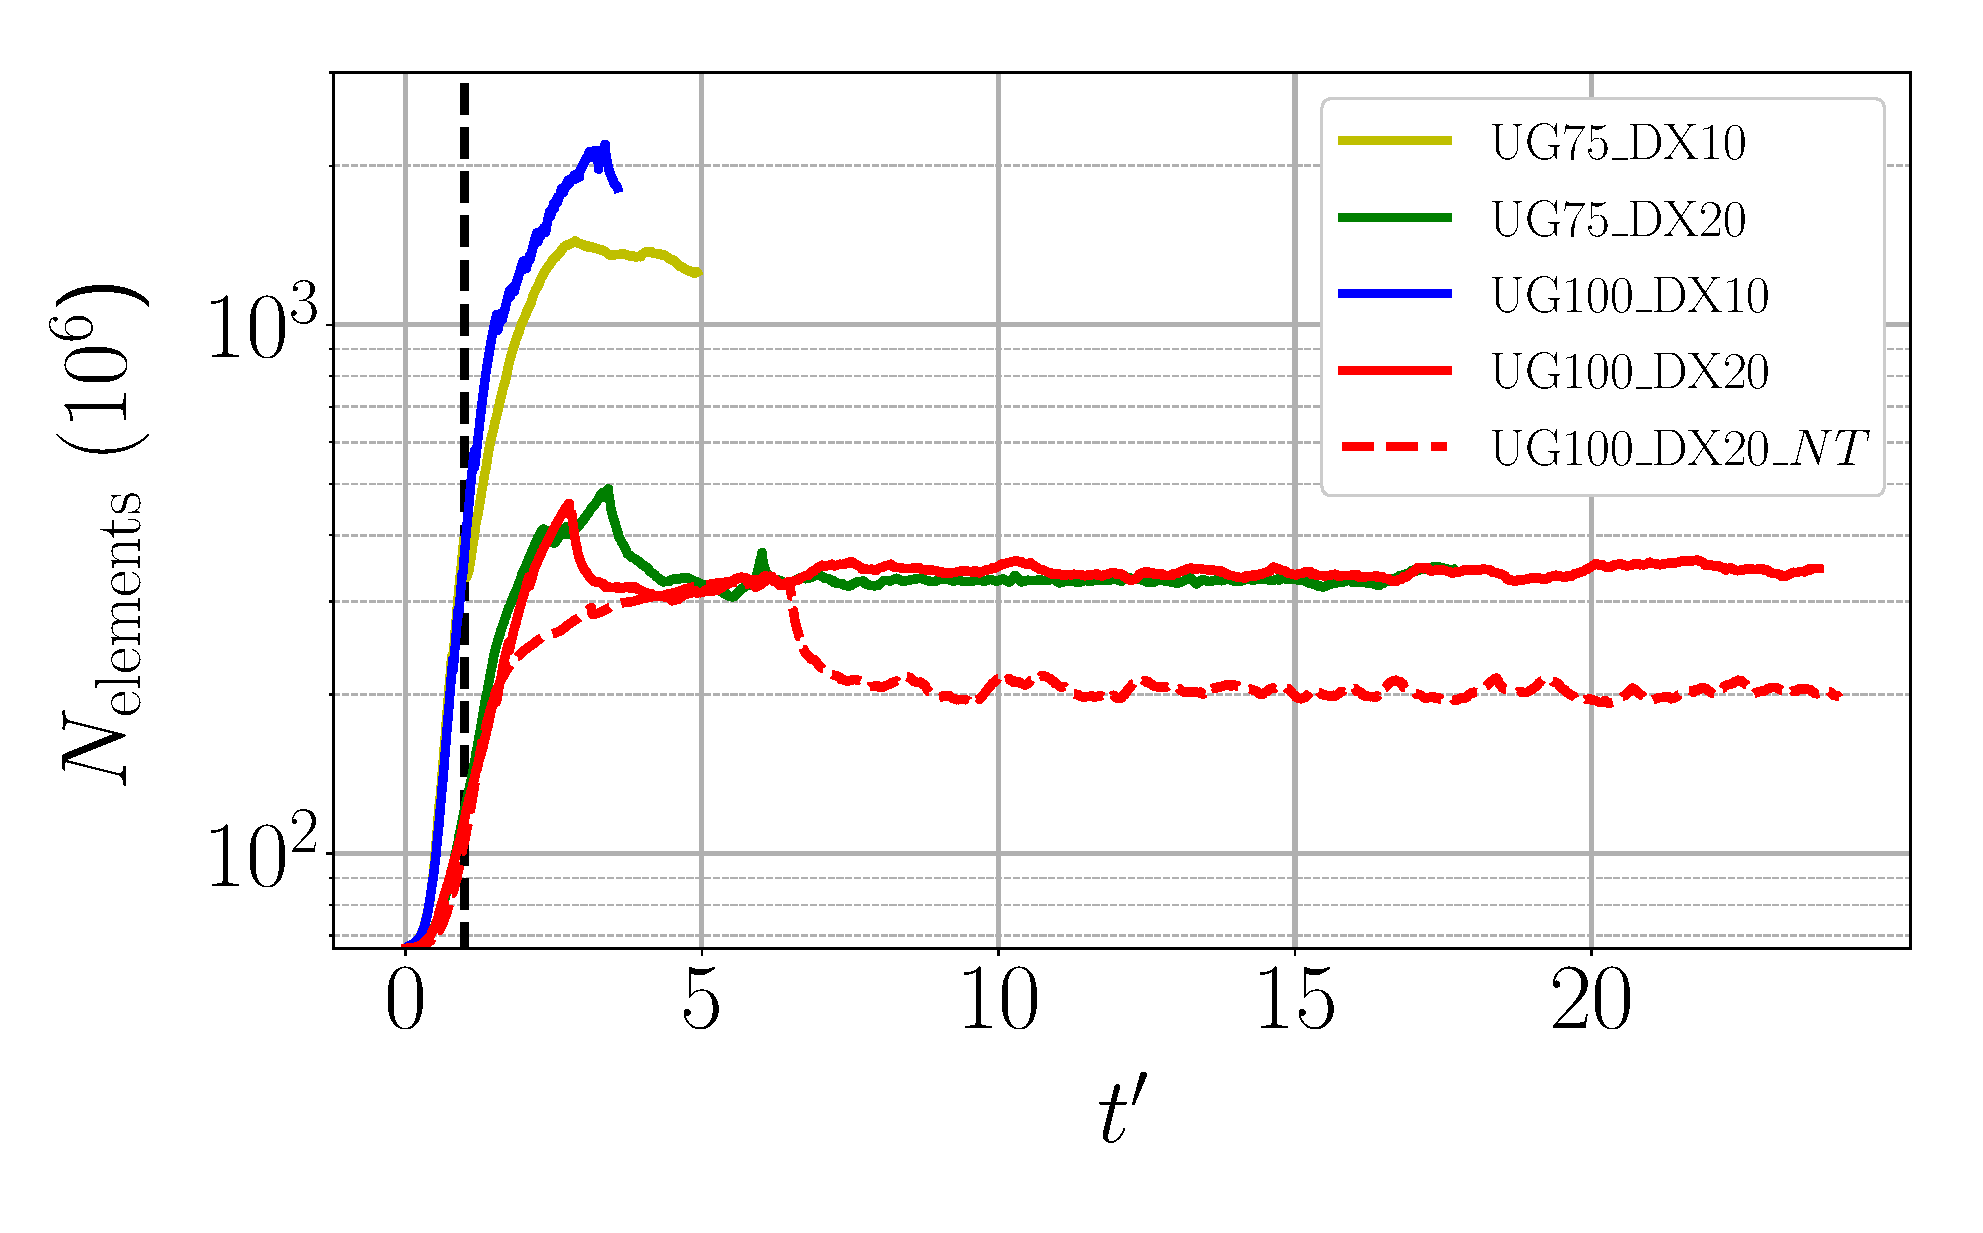
\includegraphics[scale=0.24]{./part2_developments/figures_ch5_resolved_JICF/JICF_nelem_evolution/JICF_nelem_increase}
   \vspace*{-0.25in}
   \caption{Evolution in simulations}
   \label{fig:JICF_nelem_increase_all_t} 
\end{subfigure}
\hfill
\begin{subfigure}[b]{0.45\textwidth}
	\centering
   \includegraphics[scale=0.24]{./part2_developments/figures_ch5_resolved_JICF/JICF_nelem_evolution/JICF_nelem_increase_t_in_0_2}
   \vspace*{-0.25in}
   \caption{Zoomed-in view of Figure \ref{fig:JICF_nelem_increase_all_t} in range $t^{\prime} \in [0, 2]$}
   \label{fig:JICF_nelem_increase_t_0_to_2}
\end{subfigure}

%\vskip\baselineskip
%
%\begin{subfigure}[b]{0.45\textwidth}
%	\centering
%   \includegraphics[scale=0.25]{./part2_developments/figures_ch5_resolved_JICF/JICF_nelem_evolution/JICF_nelem_increase_t_in_0_0p5}
%   \caption{Zoomed-in view in black rectangle of Figure \ref{fig:JICF_nelem_increase_t_0_to_2}}
%   \label{fig:JICF_nelem_increase_t_0_to_0p5} 
%\end{subfigure}
%\hfill
%\begin{subfigure}[b]{0.45\textwidth}
%	\centering
%   \includegraphics[scale=0.25]{./part2_developments/figures_ch5_resolved_JICF/JICF_nelem_evolution/JICF_nelem_increase_t_in_0p5_1}
%   \caption{Zoomed-in view in blue rectangle of Figure \ref{fig:JICF_nelem_increase_t_0_to_2}}
%   \label{fig:JICF_nelem_increase_t_0p5_to_0p7}
%\end{subfigure}
   \caption[Evolution of mesh size with time in JICF simulations]{Evolution of mesh size with time in JICF simulations. The dashed, black vertical line corresponds to $t^\prime = 1$, time instant when the first droplet reaches the sampling plane $x = 10$ mm.}
\label{fig:JICF_nelem_increase}
\end{figure}

\subsection{Breakup topology}
\label{subsubsec:ch5_breakup_topology}

In a liquid JICF, the most common primary atomization mechanisms are column and surface breakup (see $\S$\ref{sec:ch1_fuel_injection_technology} for a literature review on the topic). Both mechanisms are also identified in the resolved simulations performed. The \textbf{surface breakup} phenomenon is illustrated in Figure \ref{fig:jicf_surface_breakup_ug75_dx10}. Two regions are analyzed at the side of the jet: region A shows a zoomed-in view closer to the liquid injector, while region B details surface breakup taking place further downstream. Closer to the injector (region A), surface breakup is caused by lateral instabilities developed as a consequence of the strong shear force exerted by the incoming air, which forms corrugations at the surface \citepColor[behzad_surface_2016]. Droplets generated in this region do not undergo further breakup since they are very small (see the green and red ellipses, which follow the droplets generated from the corrugations) and, often, of the order of mesh resolution: most of these droplets will disappear when the levelset function is transported in the simulations. This issue is discussed later in $\S$\ref{subsec:ch5_mass_conservation_ACLS_set_levelset_band}. Further downstream (region B), the jet is more deformed and surface breakup generates ligaments that separate from the main core and then undergo classical atomization: enclosed in red, the formation process of a ligament and its breakup into three smaller, different ligaments is depicted. As shown, this process forms liquid structures which are not spherical and can undergo further atomization, even though this one still occurs close to the jet dense core and the formed structures will be in equilibrium with the ambient gas shortly afterwards.

\clearpage

\begin{figure}[ht]
\centering
\includegraphics[scale=0.175]{./part2_developments/figures_ch5_resolved_JICF/JICF_breakup/surface_breakup}
\caption{Surface breakup observed in case UG75\_DX10}
% Soluciones:
% parte arriba: sol26_15,_21, sol27_03,06
% parte abajo: sol26_15,_18,_21,_24
\label{fig:jicf_surface_breakup_ug75_dx10}
\end{figure}

\textbf{Column breakup} is depicted in Figure \ref{fig:jicf_column_breakup_ug100}, where cases UG100\_DX20 and UG100\_DX10 are shown. Jets are colored by vertical velocity $w$. This atomization mechanism is mainly caused by the instabilities developed in the windward side of the jet, which are highly dependent on the mesh resolution employed: simulations with the coarse resolution of $\Delta x_\mathrm{min} = 20$ $\mu$m do not show instabilites until the column is highly deformed far from the injector. On the contrary, the fine resolution $\Delta x_\mathrm{min} = 10$ $\mu$m resolves windward instabilities closer to the injector: these ones are propagated downstream the jet leading to its breakup. Coarse simulations do not show instabilities close to the injector, but eventually develop interfacial waves further downstream leading also to column breakup. In the fine case, instabilities are formed at the outlet of the liquid nozzle and amplified along the liquid column. Further downstream, they form sheets which are pushed by the air. The red ellipse encloses one of these sheets and follows it with time until it breaks: the sheet starts to separate from the dense core in its central region and forms tiny ligaments that break into small droplets while keeping an annular ligament with high velocity attached to the dense core by its edges. This ligament eventually separates and breaks into smaller ligaments that will continue to undergo atomization further downstream. The coarse simulation shows no instabilities at the beginning of the column, but similar topology of the produced ligaments. Ligaments from the fine simulation have a higher vertical velocity than in the coarse one. As a consequence, the liquid structures in the fine case will penetrate further, which will affect the sprays sampled further downstream. The mean trajectories from the jets, which are discussed in $\S$\ref{subsec:ch5_jet_trajectories_results}, will also reveal the difference in jet penetration with resolution. 

\subsubsection*{Resolution of instabilities}
%\label{subsec:ch5_instabilities_presence}

As aforementioned, surface instabilities are present in the jet's windward side for the fine resolution but not for the coarse one. This can be clearly observed by looking at Figures \ref{fig:JICF_establishment_UG100_lateral} to \ref{fig:JICF_establishment_UG75_top}. Previous works on resolved simulations of liquid-gas interfaces in injectors have also shown a dependency of the instabilities with the mesh resolution, such as the compound nozzle of \citeColor[cousin_primary_2012]. In this section, some possible causes of the development of windward instabilities are investigated and discussed. Three main hypothesis are thought to play a role in the formation of instabilities:

\begin{enumerate}

	\item The smallest wavelengths are of the order of the mesh resolution and can be resolved by the fine mesh, but not with the coarse one.
	
	\item The \textbf{liquid turbulence} within the nozzle is affected by the interface resolution, causing instabilities for the fine case but not for the coarse one.
	
	\item The \textbf{gaseous field} outside the nozzle is affected by the interface resolution, causing instabilities for the fine case but not for the coarse one.

\end{enumerate}


\clearpage

\begin{figure}[ht]
\centering
\includegraphics[scale=0.10]{./part2_developments/figures_ch5_resolved_JICF/JICF_breakup/column_breakup}
\caption{Column breakup phenomenon in cases UG100\_DX10, UG100\_DX20}
% Soluciones:
% dx10: sol22_03, sol23_04, sol27_00,_08, sol28_06, sol29_07
% dx20: sol09_05,_21,_37,_53,_69,_85
\label{fig:jicf_column_breakup_ug100}
\end{figure}


\subsubsection*{1) Size of smallest wavelengths}


The first hypothesis to be tested for clarifying why the coarse mesh does not resolve these liquid disturbances is that this resolution ($\Delta x_\mathrm{min} = 20~\mu$m) is not fine enough to capture the wavelenghts. To assess this, instantaneous views of the mesh and liquid-gas interface in the plane $y = 0$ mm are shown in Figure \ref{fig:JICF_instabilities_lambda}. The spatial domain corresponds to the white rectangles of Figure \ref{fig:JICF_w_mesh}. The instability in the coarse mesh is visualized downstream the jet since it is where waves start appearing, while the fine resolution captures the first instabilities evolving in the vicinity of the injector. In both cases, instabilities are present in the windward size of the jet, $\lambda$ being the size of the shortest wavelengths (i.e. the first instability developed along the jet interface). The measured wavelength is $\lambda \approx 400 ~ \mu$m for the coarse resolution $\Delta x_\mathrm{min} = 20~\mu$m, which yields a ratio $\lambda / \Delta x_\mathrm{min} = 20$. In the case of the fine resolution $\Delta x_\mathrm{min} = 10~\mu$m, the measured instability is $\lambda \approx 160 ~ \mu$m, corresponding to $\lambda / \Delta x_\mathrm{min} = 16$.  According to \citeColor[pairetti_mesh_2020], waves can be resolved with at least 4 mesh elements, i.e.  $\lambda / \Delta x_\mathrm{min} = 4$, so the instabilities are properly resolved in both cases. Indeed, the smallest instability in the fine simulation could also be resolved in the coarse one, since in this case the ratio would be $\lambda / \Delta x_\mathrm{min} = 160/20 = $ 8. Therefore, the coarse mesh is thin enough to capture the smallest instabilities, and the first hypothesis does not hold true.

\clearpage

\begin{figure}[ht]
\centering
\includeinkscape[inkscapelatex=false,scale=0.5]{./part2_developments/figures_ch5_resolved_JICF/instabilities_resolution/JICF_instabilities_lambda}
\caption[Resolution of instabilities at windward side of JICF for both resolutions in the high Weber operating point.]{Resolution of instabilities at windward side of JICF for both resolutions in the high Weber operating point. The domain depicted corresponds to the white rectangles in Figure \ref{fig:JICF_w_mesh}. }
\label{fig:JICF_instabilities_lambda}
\end{figure}

\subsubsection*{2) Liquid turbulence in nozzle}

From previous studies, it is believed that the formation of instabilities in injectors is caused by the turbulence within the injection nozzle. This holds in both two-phase problems involving liquid injectors \citepColor[wu_effects_1994,xiao_les_2014]
and in single-phase, mixing problems where one gaseous species is injected into a plenum containing a different gas, such as in gaseous jets in crossflow \citepColor[kelso_experimental_1996,karagozian_jet_2014]. \citeColor[wu_effects_1994] studied experimentally a round liquid jet in which they suppressed the boundary layer at the injector exit, finding that interface instabilities are reduced in such case. They concluded then that "\textsl{boundary layer effects, such as vorticity or variations of mean velocities from viscous effects, play a dominant role in primary breakup} (sic)".

A view of the nozzle for the high Weber case colored by the dimensionless wall distance $y^+ = y / u_\tau / \mu$, where $y$ is the distance normal to the wall and $u_\tau$ the friction velocity, is displayed in Figure \ref{fig:injector_visualization_y_plus}. Both fine and coarse resolutions are shown. The $y^+$ is a scalar magnitude representing the dimensionless distance from the first cell to the wall, and indicates the level of resolution in the vicinity of the walls: high values ($y^+ > 12$) mean that the boundary layer is poorly resolved and wall functions are needed as boundary conditions, while low values denote good resolution and wall laws can be avoided \citepColor[pope_turbulent_2000]. Figure \ref{fig:injector_visualization_y_plus} shows the $y^+$ distribution to be low in both nozzles. The PDF of the $y^+$ at the injector walls for both cases is plotted in Figure \ref{fig:jicf_nozzle_y_plus_PDF}: its magnitude is always lower than $15$, hence the wall is properly resolved in both cases and no wall functions are needed, which justifies the choice of non-slip wall boundary condition as indicated in Figure \ref{fig:numerical_setup_maquette_JICF_DLR}.  The coarse resolution shows the smallest $y^+$ to be around 4, while the fine one displays values close to 1 and a higher presence of elements with $y^+$ between 1 and 5. A zoomed-in view of this section in Figure \ref{fig:injector_visualization_y_plus} shows that the cell is finer in a region spanning $120~ \mu$m upstream the nozzle exit: here, the mesh size is $10~ \mu$m for the fine case while the coarse simulation contains elements with $20 ~\mu$m cell size. The reason is that the levelset band has been set to 12 cells from the liquid interface, and the interface is attached to the nozzle edges at the exit of the injector: the refinement extends then up to 12 cells upstream the injection point, creating a region of $120~\mu$m with cells of $10~\mu$m size. For the coarse case, the same applies but with a cell size of $20~\mu$m (and therefore a refinement region of $240~\mu$m length). As a consequence, the $y^+$ values are low in the end section of the nozzle for the fine case, yielding cells with $y^+ < 5$ (an $y^+ < 5$ indicates that the viscous sublayer, which is the closest part of the boundary layer close to the wall, is resolved) as shown by the PDF of Figure \ref{fig:jicf_nozzle_y_plus_PDF} which are not captured by the coarse case. 


\begin{figure}[ht]
\centering
\includeinkscape[inkscapelatex=false,scale=0.55]{./part2_developments/figures_ch5_resolved_JICF/instabilities_resolution/injector_visualization_y_plus}
\caption{$y^+$ distribution in the nozzle walls for high Weber cases}
\label{fig:injector_visualization_y_plus}
\end{figure}




%Besides a better resolution at the wall, the cells inside the injector far from the walls which are also comprised within the levelset band are also refined to the $\Delta x_\mathrm{min}$ value imposed.  

A cut on the $y = 0$ plane with a view on the nozzle region is displayed in Figure \ref{fig:jicf_injector_resolution_with_mesh}.  For $x < 0$ the element size field $\Delta x$ in the fine resolution simulation is shown, while the coarse one is displayed for $x > 0$. The interface outside the injector is highlighted by the white contour, and the band limits are denoted by the black contour. The metric within the band is smaller for the fine resolution, which is straightforward since this is the region with imposed $\Delta x_\mathrm{min}$. The band attaches inside the injector and refines the wall in this region, producing a better wall resolution for the fine simulation as it was shown in Figure \ref{fig:injector_visualization_y_plus}. Below the band reattachment location, the nozzle walls are not refined but the rest of the injector is, due to the transition from the cell size $\Delta x_\mathrm{min}$ to the baseline cell size (see Figure \ref{fig:AMR_strategy}). The refinement is found to extend upstream the straight section of the injector: the fine simulation contains smaller elements that the coarse one in this region, while both meshes then show similar element sizes in the tapered section of the nozzle as shown by the zoomed-in region of Figure \ref{fig:jicf_injector_resolution_with_mesh}.


\begin{figure}[ht]
	\centering
   \includegraphics[scale=0.20]{./part2_developments/figures_ch5_resolved_JICF/instabilities_resolution/y_plus_injector}
   \vspace{-0.15in}
   \caption{PDF of $y^+$ at the nozzle walls for high Weber cases}
   \label{fig:jicf_nozzle_y_plus_PDF}
\end{figure}

The improved resolution inside the last section of the nozzle as shown by Figure \ref{fig:jicf_injector_resolution_with_mesh} might have an impact on the development of turbulence in this region. Further insight is given in Figure \ref{fig:jicf_nozzle_disks}, where $TKE$ is displayed in two planes perpendicular to the flow direction at two vertical locations: $z = -0.35$ mm (in the middle of the injector, outside the levelset band refined region) and $z = 0$ mm (the nozzle exit, where cells are refined within the levelset band). The $TKE$ values are low at the center of the injector and high around the walls: in fact, the liquid Reynolds numbers $Re_l$ in the operating points considered (see Table \ref{tab:jicf_operating_conditions}) indicate laminar flow within the injector, hence the freestream liquid flow does not transition into a turbulent state and the turbulent content is null at the center of the injector. $TKE$ increases then at the walls due to the presence of the boundary layer. As observed in Figure \ref{fig:jicf_nozzle_disks}, the coarse case displays low values of $TKE$ with respect to the fine simulation, where $TKE \sim 1$ closer to the walls around all its azimuthal perimeter. The differences in the turbulent state are seen both at $z = 0$ mm and at $z = -0.35$ mm due to the nozzle refinement from the levelset band location up to the tapered section.


\begin{figure}[ht]
	\centering
   \includegraphics[scale=0.28]{./part2_developments/figures_ch5_resolved_JICF/instabilities_resolution/injector_resolution_with_mesh}
   \caption{Mesh element size $\Delta x$ shown at plane $y = 0$ for instantaneous simulations of cases UG100\_DX10, UG100\_DX20}
   \label{fig:jicf_injector_resolution_with_mesh}
\end{figure}

\begin{figure}[ht]
	\centering
   \includegraphics[scale=0.5]{./part2_developments/figures_ch5_resolved_JICF/instabilities_resolution/injector_visualization_disks}
   \caption{Planes within the injector showing TKE at locations $z = 0, -0.35$ mm for the high Weber case}
   \label{fig:jicf_nozzle_disks}
\end{figure}


The profiles of mean vertical velocity $\overline{w}$, $TKE$ and mean vorticity magnitude $|\overline{\omega}|$ obtained at the black lines from Figure \ref{fig:jicf_nozzle_disks} are plotted in Figure \ref{fig:jicf_data_lines_inside_injector}. Due to symmetry of all profiles, only the first half has been shown. The boundary layer thicknesses $\delta$ have been obtained as the points where $\overline{w}$ decrease to $99~\%$ of its value at the center ($x = 0$ mm). The $\overline{w}$ graph shows that thickness and velocity profiles depend on the resolution $\Delta x_\mathrm{min}$ employed: the fine case shows a thinner boundary layer and a steeper $\overline{w}$ profile, specially at $z = 0$ mm. The $TKE$ and mean vorticity profiles show higher contents in both within the boundary layer for the fine case: in the case of $TKE$, case UG100\_DX20 shows a peak of $0.2~J.kg^{-1}$ magnitude while case UG100\_DX10 retrieves $0.57~J.kg^{-1}$, which is almost three times larger. This higher liquid turbulent state within the injector for the fine resolution could cause the initial interface perturbations that develop into the surface instabilities observed in the fine case. Nevertheless, it is not clear whether the differences in the turbulent state are significant to trigger instabilities: even though there is a ratio of 3 between the maximum $TKE$ found among resolutions, the relation $TKE/ \left( 0.5 u_l^2 \right)$ (i.e. TKE againt bulk liquid kinetic energy) is of $0.075~\%$ for UG100\_DX20 and of $0.2~\%$ for UG100\_DX10, while turbulent liquid jets where the turbulence within the injector is thought to create the instabilities \citepColor[xiao_large_2013] yield ratios of the order of $TKE/ \left( 0.5 u_l^2 \right) \sim 2 \%$ \citepColor[tretola_effect_2021]. The ratio TKE - kinetic energy found in this work is one order of magnitudes lower than the ratios reported in literature: this could mean that liquid turbulent fluctuations do not reach the threshold level to overcome surface tension forces, meaning that they would not be the cause of the instabilities \citepColor[lee_primary_2007]. Nevertheless, this TKE threshold is not known (more research would be needed to ellucidate this value, as literature on the topic is scarce to the knowledge of the author) and such conclusion cannot be drawn from the analysis here presented.


\begin{figure}[ht]
\flushleft
\begin{subfigure}[b]{0.3\textwidth}
	\flushleft
   \includegraphics[scale=0.225]{./part2_developments/figures_ch5_resolved_JICF/instabilities_resolution/line_data_injector_uz_zm0p35}
\end{subfigure}
\hfill
\begin{subfigure}[b]{0.3\textwidth}
	\flushleft
   \includegraphics[scale=0.225]{./part2_developments/figures_ch5_resolved_JICF/instabilities_resolution/line_data_injector_TKE_zm0p35}
\end{subfigure}
\hfill
\begin{subfigure}[b]{0.3\textwidth}
	\flushleft
   \includegraphics[scale=0.225]{./part2_developments/figures_ch5_resolved_JICF/instabilities_resolution/line_data_injector_vort_zm0p35}
\end{subfigure}

\vskip\baselineskip
\vspace*{-0.4in}

\begin{subfigure}[b]{0.3\textwidth}
	\flushleft
   \includegraphics[scale=0.225]{./part2_developments/figures_ch5_resolved_JICF/instabilities_resolution/line_data_injector_uz_z0p00}
\end{subfigure}
\hfill
\begin{subfigure}[b]{0.3\textwidth}
	\flushleft
   \includegraphics[scale=0.225]{./part2_developments/figures_ch5_resolved_JICF/instabilities_resolution/line_data_injector_TKE_z0p00}
\end{subfigure}
\hfill
\begin{subfigure}[b]{0.3\textwidth}
	\flushleft
   \includegraphics[scale=0.225]{./part2_developments/figures_ch5_resolved_JICF/instabilities_resolution/line_data_injector_vort_z0p00}
\end{subfigure}

   \caption{Profiles of mean vertical velocity, $TKE$ and mean vorticity magnitude at lines located at $y = 0$ along the planes $z = -0.35,~0$ mm}
\label{fig:jicf_data_lines_inside_injector}
\end{figure}


\subsubsection*{3) Gaseous field perturbed by the jet}


%\textbf{Ver tambien refs: 2013-Xiao, 2020-zhou, 2017-zhanng}

The third hypothesis on instabilities is that a finer cell size resolves better the gaseous field perturbed at the vicinity of the liquid interface. Indeed, the liquid conditions within the injector are laminar, and \citeColor[xiao_large_2013] suggested that for laminar jets the liquid turbulence does not play a paramount role (while it does for turbulent liquid conditions) and instabilities are instead triggered by shear caused by the incoming gaseous crossflow. The influences of the interface mesh resolution $\Delta x_\mathrm{min}$ on the gas phase are then examined in the following lines.



%Another hypothesis is that the gaseous phases are different near the injector zone, since there is a growth in element size from the interface cell size $\Delta x_\mathrm{min}$ to the baseline mesh, and therefore the cells in the fine resolution located at the vicinity of the interface are also finer. This hypothesis is tested by looking at the vorticity $\omega = \frac{1}{2} \left( \nabla \times \textbf{u} \right)$ in 

Instantaneous view of the jets and plane $y = 0$ mm from cases UG100\_DX10 and UG100\_DX20 colored by the vorticity magnitude are shown in Figure \ref{fig:JICF_instabilities_vorticity}. The fine jet shows high vorticity regions along the interface due to the instabilities formed, as well as high vorticity in the bottom part of the jet at the windward side, which indicates the onset of the instabilities. The coarse jet does not display relevant vortical structures in the jet until column breakup starts taking place downstream the injection point. The zoomed-in views of the plane $y = 0$ close to the wall shows the streamlines and vorticity distribution in the gaseous field upstream the jet. Gaseous vorticity around the interface is much higher for the fine case: roll-up vortices, which are not seen in the coarse simulation, appear and disturb the interface, amplifying the instabilities (they might even be their cause, even though this cannot be fully ensured in this analysis). Horseshoe vortices, englobed by dashed red circles, are also observed at the wall upstream upstream the liquid injector. This vortex, which is a common feature in both gaseous \citemColor[kelso_experimental_1996,zhang_flow_2017] and liquid \citepColor[zhou_simulation_2020] JICF, is stronger for the coarse simulation and weaker for the fine one (despite the mesh at its location being identical in both simulations), even though it seems not to impose a significant perturbation on the gaseous streamlines, which are on the other hand perturbed by the roll-up vortices.


\begin{figure}[ht]
\flushleft
\includeinkscape[inkscapelatex=false,scale=0.75]{./part2_developments/figures_ch5_resolved_JICF/instabilities_resolution/JICF_instabilities_vorticity}
\caption[Instantaneous vorticity fields for the high Weber operating point.]{Instantaneous vorticity fields for the high Weber operating point. Streamlines are shown in the zoomed-in regions}
\label{fig:JICF_instabilities_vorticity}
\end{figure}

The vertical velotity profiles along the yellow lines $z = 0.05, 0.2$ mm represented in Figure \ref{fig:JICF_instabilities_vorticity} are shown in Figure \ref{fig:jicf_data_lines_outside_injector}. The lines span along the $x$ direction but a change of coordinate has been done to the axial coordinate $s = x - x_\mathrm{int}$, where $x_\mathrm{int}$ is the location of the interface. Closer to the wall ($z = 0.05$ mm), the $w$ profile shows slight differences among resolutions in the vicinity of the interface: the fine case retrieves higher velocity peaks in the liquid and gaseous regions, but still very close to the coarse one. In the liquid region ($s > 0$) the fine simulation reaches faster the freestrem liquid velocity than the coarse one due to a thinner, better resolved boundary layer than in the coarse simulation. In the gaseous phase the velocity profiles are distinct due to the different perturbation of the streamlines as shown in Figure \ref{fig:JICF_instabilities_vorticity}: the fine case shows negative velocities until reaching the farfield value $w = 0$, while the coarse one presents negative values larger in absolute value than the fine case up to $s \sim -0.15$ mm and then sees a increase to positive values due to the higher perturbation induced by the stronger horseshoe vortex. When looking further from the wall, at $z = 0.2$ mm, the profiles show similar behaviour within the liquid region but significant differences in the gaseous phase: for the fine resolution, the vertical velocity drops quickly with decreasing $s$ from its interface value to below $w = - 20$ m s$^{-1}$ and then relatex towards a freestream value close to 0, while the coarse one shows a less sharp gradient. The sharp gradient in the fine case is a possible source of shear force around the interface which can contribute to the development and amplification of the instabilities. Nevertheless, it is yet not clear whether this gradient is the cause of the instabilities, or it is actually caused by other factors such as the turbulence developed within the injector.


\begin{figure}[ht]
\flushleft
\begin{subfigure}[b]{0.45\textwidth}
	\flushleft
   \includegraphics[scale=0.25]{./part2_developments/figures_ch5_resolved_JICF/instabilities_resolution/line_data_outside_injector_z_low}
\end{subfigure}
\hfill
\begin{subfigure}[b]{0.45\textwidth}
	\flushleft
   \includegraphics[scale=0.25]{./part2_developments/figures_ch5_resolved_JICF/instabilities_resolution/line_data_outside_injector_z_upper}
\end{subfigure}

   \caption[Vertical velocity profiles at yellow lines depicted in Figure \ref{fig:JICF_instabilities_vorticity}]{Vertical velocity profiles at yellow lines depicted in Figure \ref{fig:JICF_instabilities_vorticity}. The black vertical line indicates the location of the interface: negative $s$ values are located in the gas phase while positive ones are in the liquid phase}
\label{fig:jicf_data_lines_outside_injector}
\end{figure}

From the analysis performed in this section, it can be stated that refining the mesh at the interface has an effect on both the liquid phase within the injector and the gaseous phase upstream the injection point. Differences have been observed in the liquid nozzle, particularly in relation to the resolution of the boundary layer in the injector walls and the turbulent magnitudes $TKE$ and vorticity: nevertheless, the differences might not be significant in absolute values to be the cause of the instabilities. A proper assessment of this statement should be done by comparing the obtained values with reference values from studies dealing with similar configurations and operating conditions, which are not present in literature nowadays to the knowledge of the authors. Observation of the gaseous phase has shown relevant differences among interface resolutions, particularly in relation to the appearance of vortical structures and shear layers around the interface which are directly linked to interfacial instabilities. However, it is not clear if these features in the gaseous field are the cause of the early development of the instabilities or a consequence of them: this one has been a fundamental question in the field of jets open for a long time \citepColor[rayleigh_instability_1878] which requires further study. %Further studies would require to analyze both hypothesis separately, something which has not been 




%As observed in Figure \textbf{XX}, ligaments generated due to instabilities in the fine resolution simulations \hl{contain a higher inertia and are stripped-off the dense core with larger velocities than those produced in the coarse resolution, where instabilities are not generated}. Such ligaments and the subsequent droplets produced from their breakup will penetrate further away in the vertical direction.

%We can see in Figure \textbf{XX} that the wavelengths $\lambda$ of the generated instabilities are ...

%When instabilities are present, primary atomization is affected and the generated ligaments \hl{contain more inertia}. As




\subsection{Jet trajectories}
\label{subsec:ch5_jet_trajectories_results}

One of the most important characteristics of a jet in crossflow is its trajectory (see $\S$\ref{sec:ch1_fuel_injection_technology}). This feature determines how far the jet penetrates in the domain and has a paramount effect on the latter evaporation and mixing processes, hence affecting flame dynamics in reactive cases. Experimental studies often provide correlations for the trajectory of the windward side of the jet (see Table \ref{tab:correlations_experimental_JICF}). This is the side indicating the furthest vertical location ($z$) containing liquid for each axial location in crossflow direction ($x$). Correlations relating $z$ and $x$ are often specified for a specific operating range ($q$ and $We$ limits) and up to a certain axial location downstream the injection point. 

In this section, trajectories for the jets from the resolved simulations are going to be analyzed and compared with an experimental correlation. Four post-processing methods for obtaining trajectories are proposed and discussed. Then, these methods are applied to one computation for illustrating their differences. Finally, one method is selected (based on its similarity with the experimental processing methodologies) for comparing the trajectories among simulations.

%Different methods to obtain trajectories from resolved simulations were proposed in $\S$\ref{sec:ch5_tools_jicf_trajectories}. These methods are summarized in Table \ref{tab:jicf_tools_trajectories_obtention}. In this section, firstly  the four methods described are applied to the simulation UG100\_DX20, the trajectories obtained are then compared and discussed. Secondly, the method MEAN\_GRAD is chosen to perform experimental validation with all simulations from Table \ref{tab:jicf_resolved_simulations_performed}. \hl{Finally, a comparison of the $L_2$ errors based on the maximum distance downstream in the trajectory ...}



\subsubsection*{Processing methodologies for jet trajectories}	%\label{sec:ch5_tools_jicf_trajectories}


Experimentally, researchers have used different approaches to obtain trajectories based on the different optical techniques employed. Many works \citemColor[becker_breakup_2002,stenzler_penetration_2003,freitag_spray_2008] take instantaneous images of the jet with shadowgraphy techniques and then MIE scattering or emboss-filter operations to obtain binary images where liquid and gas phases can be clearly distinguished. Then, images are averaged and the vertical penetration is obtained by detecting the coordinates where the light intensity gradients are maximum. Image averaging can be performed before or after the filtering operations. Such methods obtaining trajectories from average images are hereafter denoted as \textbf{mean trajectory methods}. Figure \ref{fig:expe_obtention_of_trajectories} shows an illustration of such experimental methodology from the work by \citeColor[stenzler_penetration_2003]. Other works \citepColor[ragucci_trajectory_2007] use the same principles of filtering and binarization, but obtain the trajectories from instantaneous jet images. Then, instantaneous trajectories are averaged to yield the mean trajectories. These methods are hereafter denoted as \textbf{instantaneous trajectory methods}.

\begin{figure}[ht]
     \centering
     \includeinkscape[inkscapelatex=false,scale=0.6]{./part2_developments/figures_ch5_resolved_JICF/trajectories_obtention/expe_obtention}
     \caption{Illustration of experimental procedure to obtain trajectories. Figures taken from \citeColor[stenzler_penetration_2003]}
      \label{fig:expe_obtention_of_trajectories}
\end{figure}

From a computational perspective, similar methodologies can be applied to obtain the jet trajectories from simulations. The same sequence of operations from Figure \ref{fig:expe_obtention_of_trajectories} for processing experimental images could be applied to numerical snapshots of the JICF. Nevertheless, the ACLS methodology presents the advantage that the interface is clearly defined with the $\psi$ function, and hence trajectories can be obtained with different methods without the need to use MIE scattering and binarization (steps 2 and 3 from Figure \ref{fig:expe_obtention_of_trajectories}). In this work, four methodologies to obtain the numerical trajectories from JICF resolved simulations are presented. As in the experimental classification previously suggested to obtain trajectories, these methodologies are also distinguished as \textbf{mean trajectory methods} or \textbf{instantaneous trajectory methods}, depending on whether they use the mean or instantaneous $\psi$ field respectively. Two methods for each category are detailed in this section.



\paragraph*{Mean trajectory methods}

One possibility to obtain mean trajectories is by using the mean field of the levelset function, $\overline{\psi}$. An example of a converged $\overline{\psi}$ field is shown in Figure \ref{fig:trajectory_obtention_mean_methods_c_d} left. This requires the accumulation of statistics over a certain time (instantaneous trajectories do not need statistics accumulation as long as the instantaneous $\psi$ field is available), but presents the advantage that the jet trajectory can be obtained with one single $\overline{\psi}$ field once convergence is achieved. In this category, two different methods are used: the \textbf{maximum gradient method} and the \textbf{iso-contour method}:


\begin{itemize}

	\item The \textbf{maximum gradient method} consists to obtain the maximum gradient of $\overline{\psi}$ in the vertical direction for each $x$ coordinate: $\max \left( \nabla_z | \overline{\psi} | \right)$. Figure \ref{fig:trajectory_obtention_mean_methods_c_d} center shows an example of a $\max \left( \nabla_z | \overline{\psi} | \right)$ contour. This method is more similar to the experimental methods presented in \citeColor[becker_breakup_2002], \citeColor[stenzler_penetration_2003] and \citeColor[freitag_spray_2008]: in these works, the jet trajectory is obtained as the contour of the maximum intensity gradient in the vertical direction of the mean jet (see Figure \ref{fig:expe_obtention_of_trajectories}).
	
	\item Trajectory as \textbf{iso-contour} of mean levelset field $\overline{\psi}$. This approach has been used to obtain JICF trajectories with simulations using a VOF methodology \citepColor[desclaux_experimental_2020]. In this work, several values for the iso-contour have been tested, and it has been found that the mean trajectories obtained are very sensitive to this value. Finally, a value of $\overline{\psi} = 0.01$ has been identified as the best contour to compare the resulting trajectories with the ones obtained with the rest of methods. Figure \ref{fig:trajectory_obtention_mean_methods_c_d} right shows an example of a an example of a $\overline{\psi} = 0.01$ contour.


\end{itemize}

\begin{figure}[ht]
     \centering
     \includeinkscape[inkscapelatex=false,scale=0.35]{./part2_developments/figures_ch5_resolved_JICF/trajectories_obtention/methods_c_d_and_mean_psi_field}
     \caption[Methods based on mean trajectories]{Methods based on mean trajectories. \textsl{Left}: $\overline{\psi}$ field. \textsl{Center}: $\max \left( \nabla_z | \overline{\psi} | \right)$ contour. \textsl{Right}: contour $\overline{\psi} = 0.01$.}
	% See: https://stackoverflow.com/questions/35210337/can-i-plot-several-histograms-in-3d/35225919
      \label{fig:trajectory_obtention_mean_methods_c_d}
\end{figure}


\paragraph*{Instantaneous trajectory methods}

Instead of using the mean levelset field, the averaged numerical trajectories can be obtained from instantaneous solutions of the jet by firstly getting the instantaneous trajectories and then averaging them. Figure \ref{fig:trajectory_obtention_instantaneous_general} shows the procedure to extract the interface contour that is later used to obtain the trajectories. First, the liquid-gas interface is plotted in the domain as a surface of iso-contour $\Gamma: \psi = 0.5$ (Figure \ref{fig:trajectory_obtention_instantaneous_general} left), and then this contour is extracted at the central plane $y = 0$, as indicated by the black line of Figure \ref{fig:trajectory_obtention_instantaneous_general} right. 

\begin{figure}[h]
     \centering
     \begin{subfigure}[b]{0.45\textwidth}
         \centering
         \includeinkscape[inkscapelatex=false,scale=0.35]{./part2_developments/figures_ch5_resolved_JICF/trajectories_obtention/instantaneous_interface_3D}
         %\caption{Instantaneous jet interface}
     \end{subfigure}
     %\hfill
     \begin{subfigure}[b]{0.45\textwidth}
         \centering
         \includeinkscape[inkscapelatex=false,scale=0.35]{./part2_developments/figures_ch5_resolved_JICF/trajectories_obtention/instantaneous_interface_y0}
         %\caption{Contour of instantaneous interface at plane y = 0}
     \end{subfigure}
        \caption[Procedure to obtain instantaneous trajectories.]{Procedure to process instantaneous trajectories. \textsl{Left}: instantaneous jet interface. \textsl{Right}: contour of instantaneous interface at plane y = 0}
	% See: https://stackoverflow.com/questions/35210337/can-i-plot-several-histograms-in-3d/35225919
        \label{fig:trajectory_obtention_instantaneous_general}
\end{figure}

Once the interface is obtained at $y = 0$, the outer contour of the trajectory must be obtained. This is the one corresponding to the windward side of the jet, and hence the one defining the instantaneous trajectory. For its obtention, the $z$ axis is swept and the points belonging to the trajectory are obtained as follows:

\begin{enumerate}

	\item The $z$ axis is discretized in intervals with constant thickness.
	
	\item For each interval, the contour point with minimum $x$ coordinate is obtained.
	
	\item Points are sorted according to their $x$ coordinate, defining the trajectory.

\end{enumerate}

This procedure is repeated at every instantaneous snapshot of the jet to obtain the corresponding trajectories. Then, all  trajectories are interpolated in the same axial locations and averaged to yield mean trajectories which can be compared to experimental correlations. This method is similar to the experimental methodology employed by \citeColor[ragucci_trajectory_2007], and was used by \citeColor[leparoux_primary_2018] to simulate their experimental configuration and validate the computations. However, it differs from the methodology employed by \citeColor[becker_breakup_2002], whose experimental test rig is simulated in this work and who obtained the trajectories with a methodology more similar to the mean trajectory methods (see next point). Still, it is worth to investigate the instantaneous methodologies and to compare them with the mean methods to illustrate the effect that the post-processing methodology can have on the jet trajectories when treating the same simulations.

The procedure previously described works properly in the dense core, where the interface contour is continuous up to the breakup point $z_b$. After this location, atomization takes place and the detected interface contours belong to ligaments or droplets. In this case, the definition of \textsl{outer trajectory} does not hold as clearly as in the dense core: some contours detected might belong to satellite droplets or to drops originated from surface breakup, and could modify the final average trajectory by lowering it down. With this consideration, two different trajectories are distinguished in the instantaneous methodologies: \textbf{non-monotonic} and \textbf{monotonic} trajectories:

%\subsubsection*{Non-monotonic trajectory}

\begin{itemize}

	\item \textbf{Non-monotonic instantaneous trajectories} can be obtained by applying the methodology as explained in the previous lines, accounting also for the contours which a priori do not pertain to the instantaneous trajectory. This procedure is illustrated in Figure \ref{fig:trajectory_obtention_instantaneous_method_a}: the different points of the trajectory are obtained when sweeping the $z$ axis, and the instantaneous trajectory is obtained by joining these points. Then, sorting all the sampled points along the $x$ axis creates a non-monotonic trajectory since some contour points belong to liquid structures further downstream, see Figure \ref{fig:trajectory_obtention_instantaneous_method_a} right.

\begin{figure}[ht]
     \centering
     \begin{subfigure}[b]{0.45\textwidth}
         \centering
         \includeinkscape[inkscapelatex=false,scale=0.35]{./part2_developments/figures_ch5_resolved_JICF/trajectories_obtention/method_a_sweep_nonMonotonic}
         %\caption{Instantaneous jet interface}
     \end{subfigure}
     %\hfill
     \begin{subfigure}[b]{0.45\textwidth}
         \centering
         \includeinkscape[inkscapelatex=false,scale=0.34]{./part2_developments/figures_ch5_resolved_JICF/trajectories_obtention/method_a_inst_trajectory}
         %\caption{Contour of instantaneous interface at plane y = 0}
     \end{subfigure}
        \caption[Obtention of non-monotonic instantaneous trajectory]{Obtention of non-monotonic instantaneous trajectory. \textsl{Left}: sweep process along z axis of interface points. \textsl{Right}: instantaneous trajectory.}
	% See: https://stackoverflow.com/questions/35210337/can-i-plot-several-histograms-in-3d/35225919
        \label{fig:trajectory_obtention_instantaneous_method_a}
\end{figure}

\item \textbf{Monotonic instantaneous trajectories} are obtained similarly to non-monotonic ones but with one fundamental difference: when sorting along the $x$ axis, only points with increasing $z$ coordinate are considered. In this way, a monotonic trajectory is obtained, see Figure \ref{fig:trajectory_obtention_instantaneous_method_b} right. 


\begin{figure}[ht]
     \centering
     \begin{subfigure}[b]{0.45\textwidth}
         \centering
         \includeinkscape[inkscapelatex=false,scale=0.35]{./part2_developments/figures_ch5_resolved_JICF/trajectories_obtention/method_b_sweep_monotonic}
         %\caption{Instantaneous jet interface}
     \end{subfigure}
     %\hfill
     \begin{subfigure}[b]{0.45\textwidth}
         \centering
         \includeinkscape[inkscapelatex=false,scale=0.33]{./part2_developments/figures_ch5_resolved_JICF/trajectories_obtention/method_b_inst_trajectory}
         %\caption{Contour of instantaneous interface at plane y = 0}
     \end{subfigure}
        \caption[Obtention of monotonic instantaneous trajectory]{Obtention of monotonic instantaneous trajectory. \textsl{Left}: sweep process along z axis of interface points, excluding points whose vertical location is lower than the vertical location of the previous ones. \textsl{Right}: instantaneous trajectory.}
	% See: https://stackoverflow.com/questions/35210337/can-i-plot-several-histograms-in-3d/35225919
        \label{fig:trajectory_obtention_instantaneous_method_b}
\end{figure}

\end{itemize}


% The two instantaneous methodologies described here will provide the same trajectories in the dense core, but will differ after the breakup point. Therefore, the trajectories obtained from this methodology can be compared and used to estimate an average position of the dense core. 



Table \ref{tab:jicf_tools_trajectories_obtention} shows a summary of the four methodologies presented, and the names used in $\S$\ref{subsec:ch5_jet_trajectories_results} to display the results.

\begin{table}[!h]
\centering
\caption{Summary of methods for computing JICF trajectories}
\begin{tabular}{ccc}
\thickhline
Group & Method & Name \\
\thickhline
\multirow{2}{*}{Instantaneous} & Non-monotonic & INST\_NM \\
 & Monotonic & INST\_M \\
 \hline
\multirow{2}{*}{Mean} & Maximum gradient & MEAN\_GRAD \\
 & Iso-contour & MEAN\_CONT \\
\thickhline
\end{tabular}
\label{tab:jicf_tools_trajectories_obtention}
\end{table}

\subsubsection*{Results}

The trajectories obtained from the computations will be compared to the experimental correlation obtained by \citeColor[becker_breakup_2002], given by the following expression.:

\begin{equation}
    \label{eq:jicf_trajectory_becker}
    \frac{z}{d_\mathrm{inj}} = 1.57 \mathrm{q}^{0.36} \ln \left( 1 + 3.81 \frac{x}{d_\mathrm{inj}} \right)
\end{equation}

which is valid for $1 < q < 12$, $90 < We_\mathrm{ae} < 2120$ and $x/d_\mathrm{inj} < 22$. For the simulations studied, $d_\mathrm{inj} = 0.45$ mm and $q = 6$. The authors also present a standard deviation for the correlation of $\sigma = 0.81$. Numerical trajectories can be plotted together with Eq. (\ref{eq:jicf_trajectory_becker}) to provide a qualitative comparison of the computations. For further insight, a quantitative measure for the difference between simulations and experiments can be introduced through a $L_2$ norm:

\begin{equation}
\label{eq:L2_JICF}
    L_2 = \sqrt{\frac{1}{N}   \sum_{i=1}^N \left( \frac{z}{d_\mathrm{inj}} \Bigr|_{\mathrm{num},i} -   \frac{z}{d_\mathrm{inj}} \Bigr|_{\mathrm{exp},i} \right)^2}
\end{equation}

where $N$ is the number of points along the abscissa $x$ in which the difference between curves is evaluated and i refers to the $i$-th point. The subscript num$,i$ indicates the mean value obtained from simulations for the vertical location at point $i$, while exp$,i$ indicates the equivalent measure from experiments. From this definition it follows that the $L_2$ error is a measure of the deviation from experiments: the lower the $L_2$, the closer the simulation results are to the experimental ones. The $L_2$ error can also be monitored with time to determine the convergence evolution of the trajectories. \\


In first place, the four methodologies are compared by applying them to simulation UG100\_DX20, since this is the one that has run for longer physical time. The resulting trajectories are shown in Figure \ref{fig:JICF_trajectories_and_L2_comparison}a. In the vicinity of the injector all trajectories follow the same tendency up to $x/d_\mathrm{inj} \sim 1$. After this point, two different tendencies are observed: mean $\psi$ trajectories keep on following the experimental correlation, while instantaneous ones are located below. The former are noisy due to numerical dissipation in the $\psi$ field, while the latter present a smoother shape since they are obtained by interpolating instantaneous trajectories and averaging them with time. The different trends shown by the trajectories from both methodologies are due to their underlying definitions: instantaneous-averaged trajectories intend only to retrieve the outer contour of the jet, while the mean-based methods take the $\overline{\psi}$ field defined in all the domain and then obtain the trajectories at plane $y = 0$. The $\overline{\psi}$ field is diffused as opposed to the $\psi = 0.5$ contour retrieved by the instantaneous methods, so the trajectories obtained as $\max \left( \nabla_z | \overline{\psi} | \right)$ (maximum gradient) and $\overline{\psi} = 0.01$ (contour) are located in the regions where $\overline{\psi}$ is close to $0$ (i.e. where the mean presence of liquid is low). Consequently, trajectories penetrate further away than the instantaneous averaged ones in the near-injector region (coherent liquid) while they show the opposed tendency downstream after atomization has taken place (dispersed phase liquid) \\

\clearpage


\begin{figure}[ht]
\flushleft
\hspace{-0.5in}
\begin{subfigure}[b]{0.45\textwidth}
	\flushleft
   \includegraphics[scale=0.25]{./part2_developments/figures_ch5_resolved_JICF/results_trajectories/methods_comparison_trajectories_q6uG100_dx20.pdf}
   \vspace*{-0.25in}
   \caption{Mean trajectories}
   %\label{} 
\end{subfigure}
\hspace{0.25in}
%\vspace{-0.25in}
\begin{subfigure}[b]{0.45\textwidth}
	\flushleft
   \includegraphics[scale=0.25]{./part2_developments/figures_ch5_resolved_JICF/results_trajectories/methods_comparison_L2_evolution_q6uG100_dx20_shared_y_axis.pdf}
   \vspace*{-0.25in}
   \caption{$L_2$ error evolution for two $x/d_\mathrm{inj}$ ranges}
   %\caption{$L_2$ error evolution }
   %\label{}
\end{subfigure}
\caption{Trajectories and $L_2$ errors obtained with different methods for case UG100\_DX20}
\label{fig:JICF_trajectories_and_L2_comparison}
\end{figure}

The evolution of the $L_2$ norm calculated with Eq. (\ref{eq:L2_JICF}) is shown in Figure \ref{fig:JICF_trajectories_and_L2_comparison}b for all methods. The norm is calculated for two ranges in the $x$ axis: $x/d_\mathrm{inj} < 10$ and $x/d_\mathrm{inj} < 20$. The former (reduced range) considers the trajectories closer to the injector before a full disperse spray is present, and all $L_2$ norms show convergence. The norms from the instantaneous trajectories show similar values since the trajectories for $x/d_\mathrm{inj} < 10$ are always close. The mean field trajectories show noisier signals, with the case MEAN\_CONT yielding the lowest errors. When considering the range $x/d_\mathrm{inj} < 20$, the signals show different behaviours. Regarding the instantaneous-averaged trajectories, both show the same tendencies as in the reduced range, but with larger norms due to the divergence of both curves in the dispersed phase region. The trajectory from method MEAN\_CONT shows also convergence in the norm, but with a larger value than for the reduced range. On the other hand, the signal from method MEAN\_GRAD does not show convergence with time when the dispersed spray region is included. The reason is that the field $\nabla_z | \overline{\psi} |$ shows a very unstable behaviour with time in the dispersed spray, as opposed to the field $\overline{\psi}$. It is not sure whether this method will yield a converged $L_2$ if the simulation were run longer. The results from Figure \ref{fig:JICF_trajectories_and_L2_comparison} show the strong influence that the choice of trajectory obtention method can have on the results.  \\

For validating experimentally the trajectories from the rest of the simulations, the method MEAN\_GRAD is selected due to its similarity with the methodology followed by \citeColor[becker_breakup_2002] to obtain the experimental correlation. Results are shown in Figure \ref{fig:JICF_trajectories_validation} for both operating points, including the case for the high $We$ number without synthetic turbulence injection. The evolution of the $L_2$ norm displayed has been obtained for the range $x/d_\mathrm{inj} < 10$. Additionally, an error along the trajectory  $\varepsilon_i$ is also defined to indicate the trajectory’s accuracy along the crossflow’s direction $x$:

\begin{equation}
\label{eq:error_along_trajectory}
\varepsilon_i  =  \frac{ z/d_\mathrm{inj} \Bigr|_{\mathrm{num},i} - z/d_\mathrm{inj} \Bigr|_{\mathrm{exp},i} }{ z/d_\mathrm{inj} \Bigr|_{\mathrm{exp},i} }
\end{equation}



Trajectories are shown in Figures \ref{fig:JICF_trajectories_validation}a and b for both operating points. The first remarkable events are the dependence on mesh resolution for both operating points, and the differentiation of two regions with axial distance along the trajectories. From the graphs, the regions can be distinguished as follows:

\begin{enumerate}

	\item A first near-injector region in which both resolutions coincide with the experimental correlation, showing no dependence on the mesh resolution. This regions extends up to $x/d_\mathrm{inj} \sim 5$ for low $We$ and to $x/d_\mathrm{inj} \sim 4$ for high $We$. Here, the dense core is located and primary atomization takes place, resulting in an accurate trajectory prediction.
	
	\item After the near-injector region, trajectories diverge and show different trends: the coarse simulation underestimates the experimental correlation, while the fine one continues within the confidence interval of the experiments until it surpasses it. This is the region where secondary atomization is forming droplets and a dispersed spray starts to be formed, hence mispredicting the experimental correlations.

\end{enumerate}

\clearpage



\begin{figure}[ht]
\flushleft
\begin{subfigure}[b]{0.45\textwidth}
	\centering
   \includegraphics[scale=0.25]{./part2_developments/figures_ch5_resolved_JICF/results_trajectories/methods_expe_validation_trajectories_q6uG75.pdf}
   \vspace*{-0.25in}
   \caption{Low $We$ trajectories}
   %\label{} 
\end{subfigure}
%\hfill
\hspace{0.25in}
\begin{subfigure}[b]{0.45\textwidth}
	\centering
   \includegraphics[scale=0.25]{./part2_developments/figures_ch5_resolved_JICF/results_trajectories/methods_expe_validation_trajectories_q6uG100.pdf}
   \vspace*{-0.30in}
   \caption{High $We$ trajectories}
   %\label{}
\end{subfigure}

\vskip\baselineskip
\vspace*{-0.2in}

\begin{subfigure}[b]{0.45\textwidth}
	\centering
   \includegraphics[scale=0.25]{./part2_developments/figures_ch5_resolved_JICF/results_trajectories/methods_expe_validation_L2_evolution.pdf}
   \vspace*{-0.25in}
   \caption{Evolution of $L_2$ norms with time.}
   %\label{} 
\end{subfigure}
%\hfill
\hspace{0.25in}
\begin{subfigure}[b]{0.45\textwidth}
	\centering
   \includegraphics[scale=0.25]{./part2_developments/figures_ch5_resolved_JICF/results_trajectories/methods_expe_validation_error_with_xD.pdf}
   \vspace*{-0.30in}
   \caption{Error $\varepsilon$ along trajectory}
   %\label{}
\end{subfigure}


\caption{Trajectories and errors obtained with method MEAN\_GRAD}
\label{fig:JICF_trajectories_validation}
\end{figure}

\vspace*{-0.05in}

The reason why coarse simulations underestimate the trajectory further downstream, while the fine ones overestimate it, is the resolution of instabilities in the windward side of the jet (discussed previously in $\S$\ref{subsubsec:ch5_breakup_topology}).  Instabilities in the fine simulations create ligaments and droplets with high vertical velocities that penetrate further away than those generated in the coarse simulations. Consequently, their resulting trajectories penetrate further than the coarse ones and the experimental correlation after breakup occurs. 


Regarding the effect of injecting turbulence at the gaseous inlet, the red lines of Figure \ref{fig:JICF_trajectories_validation}b show that the mean trajectory is not affected when turbulence is added. The turbulence levels (as calculated in Appendix \ref{app:gas_initial_cond_JICF}) do not have an influence on the formation of instabilities for the case studied. Nevertheless, only the coarse resolution has been simulated without turbulence injection: further studies could include a simulation with a finer resolution in order to determine if the injected turbulence have an effect on the instabilities formed in the windward side of the column.

Figure \ref{fig:JICF_trajectories_validation}c shows the $L_2$ norm evolution. The coarse cases show convergence while the fine ones are still fluctuating, yet they seem to stabilize (simulations should run longer to confirm this). The final values of the errors are summarized in Table \ref{tab:jicf_L2_errors}, confirming that smaller deviations are obtained for fine resolutions. Finally, the relative error along the trajectory $\varepsilon$ is displayed in Figure \ref{fig:JICF_trajectories_validation}d. Negative values indicate underestimation of the experimental correlation, while positive ones indicate overestimation. In the vicinity of the injection nozzle ($x = 0$), errors are large because the denominator of Eq. (\ref{eq:error_along_trajectory}) is small. Then, deviations are small in the near injector region and start to increase monotonically in absolute value further downstream. Fine simulations present positive erros since they overestimate the experimental correltion, while the coarse ones yield negative ones due to the underestimation. This graph is useful to get an idea on the error commited in the vertical boundary of the spray when placing an SLI. For instance, if an injector is placed at $x = 5$ mm ($x/d_\mathrm{inj} \sim 11$), an SLI obtained from the fine resolution would yield low errors ($\sim 0~\%$ for UG75\_DX10 and $\sim 10~\%$ for UG100\_DX10), but very high ones for a coarse injector ($\sim - 25~\%$). %Placing an injector further downstream would increase the errors for any resolution. These effects will be studied in Chapter \ref{ch6:jicf_lgs_simulations}.



\begin{table}[!h]
\centering
\caption{$L_2$ errors for JICF simulations performed.}
\vspace*{-0.1in}
\begin{tabular}{cccccc}
\thickhline
\textbf{Case} &  UG75\_DX10 & UG75\_DX20 & UG100\_DX10 & UG100\_DX20 &  UG100\_DX20\_NT \\
\hline
$L_2$ & 0.29 & 1.16 & 0.44 & 1.40 & 1.35 \\
\thickhline
\end{tabular}
\label{tab:jicf_L2_errors}
\end{table}








\clearpage



\subsection{Turbulent structures in the gaseous field}
\label{ch5:subsec_turbulent_structures_in_gaseous_field}


Resolved simulations capture the liquid dense core, which perturbs the incoming air and creates turbulence downstream the injector. This perturbation effect is illustrated in Figure \ref{fig:jet_air_interaction_up_and_skeleton}. At the left, the instantaneous axial velocity fluctuations $u'$ and the jet interface in the middle plane y = 0 are plotted. The dense core creates turbulence downstream the injection point, as shown by the strong fluctuations. Such perturbations can have a great impact on secondary atomization and spray dispersion once atomization has taken place. Therefore, modelling this perturbance effect as accurate as possible is paramount for later performing dispersed-phase simulations (Chapter \ref{ch6:jicf_lgs_simulations}), where the dense core is a priori neglected and a developed spray is injected. A three-dimensional view of the perturbation effect is depicted in Figure \ref{fig:jet_air_interaction_up_and_skeleton} right, where the gaseous streamlines are visualized. Two main turbulent structures appear: a horseshoe vortex formed at the wall right upstream the liquid jet, widely observed in literature dealing with both gaseous and liquid JICF \citemColor[fric_vortical_1994,karagozian_transverse_2010,schlegel_contributions_2011], and a recirculation zone right downstream the jet. The latter, which is a is characteristic of JICF configurations at high gaseous velocities \citepColor[fontes_improved_2019], might entrap droplets emanating from the ligaments formed during column breakup and affect their trajectory and their subsequent secondary breakup. 

\begin{figure}[ht]
\flushleft
\includeinkscape[inkscapelatex=false,scale=1.1]{./part2_developments/figures_ch5_resolved_JICF/turbulent_structures/jet_air_interaction_up_and_streamlines_vortices}
\caption[Interaction between liquid dense core and gaseous phase.]{Interaction between liquid dense core and gaseous phase. \textsl{Left}: Instantaneous $u'$ field in a JICF simulation from case UG100\_DX20. The black contours indicate the lines with zero instantaneous fluctuation $u' = 0$, while the white contours denote the location of the interface at the plane. \textsl{Right}: 3D streamlines in case UG100\_DX20}
\label{fig:jet_air_interaction_up_and_skeleton}
\end{figure}


In this section, the turbulent structures created as a consequence of the dense core presence are studied. These results will be used in Chapter \ref{ch6:jicf_lgs_simulations} to compare with the disturbance effects in the gaseous field modelled in the dispersed phase simulations. The gaseous field is investigated by analyzing the mean axial gaseous velocity field $\overline{u}$ in the planes illustrated in Figure \ref{fig:jicf_sps_with_gaseous_planes}. %These planes are: the symmetry plane $y = 0$ mm, planes perpendicular to the crossflow $x = 5, 10$ mm (which correspond to the planes where spray has been sampled and postprocessed, see Figure \ref{fig:jicf_interior_boundaries_surface_measurements}), and the planes perpendicular to the injection directions $z = 0.2, 0.8, 1.6$ mm. 


\begin{figure}[h!]
	\centering
	\includeinkscape[inkscapelatex=false,scale=0.8]{./part2_developments/figures_ch5_resolved_JICF/turbulent_structures/jicf_sps_with_gaseous_planes}
	\caption{Jet from case UG100\_DX10 showing planes to study the gaseous phase}
	% NOTA: figura de pilotage 2021_05_21
	% OJO: mirar pilotages  reunion_Thierry_2021_01_22, 2021_02_04, 2021_05_21, 2021_05_25 
	\label{fig:jicf_sps_with_gaseous_planes}
\end{figure}


Mean axial velocity at the symmetry plane $y = 0$ mm for all cases are shown in Figure \ref{fig:JICF_turbulent_structures_plane_y0} (case UG100\_DX20\_NT  is not displayed in this section since its mean fields are identical to those of case UG100\_DX20). The region with mean liquid obtained as $\overline{\psi} > 0.5$ is denoted in grey, hence the displayed velocities correspond only to the mean gaseous region. Streamlines are also shown to indicate the flow direction. In all cases, a recirculation bubble enclosed by the white solid line is retrieved immediately downstream the dense core. This recirculation region is fully converged for the coarse cases but not for the fine ones. The effect of this bubble is to push the streamlines below and behind it upwards, hence confering the gas a positive vertical velocity downstream the dense core. Upstream the jet, the streamlines are initially oriented towards the axial direction but then bend vertically due to the presence of the dense core. These streamlines are again directed vertically due to the action of the recirculation bubble. In general, velocities are larger for the high Weber operating point except in the recirculation bubble, where mean negative axial velocities show the same values for both conditions.

\begin{figure}[ht]
\centering
   \includeinkscape[inkscapelatex=false,scale=0.2]{./part2_developments/figures_ch5_resolved_JICF/turbulent_structures/planes_y_ux_mean}

\caption[Mean axial velocity at plane $y = 0$ mm]{Mean axial velocity at plane $y = 0$ mm. Black lines with arrows are in-plane mean streamlines; the white solid line indicates the contour $\overline{u} = 0$ which delimites the recirculation bubble. The grey area  indicates the mean liquid region, identifed as $\overline{\psi} > 0.5$}
\label{fig:JICF_turbulent_structures_plane_y0}
\end{figure}

The $\overline{u}$ profiles along the dashed lines from Figure \ref{fig:JICF_turbulent_structures_plane_y0} are represented in Figures \ref{fig:JICF_sps_lines_y0_along_x_ux_mean} and  \ref{fig:JICF_sps_lines_y0_along_z_ux_mean}. Both graphs reveal that perturbations are stronger closer to the bottom wall (line $z = 1.6$ mm in Figure \ref{fig:JICF_sps_lines_y0_along_x_ux_mean}  traverses indeed the recirculation bubble, since velocities reach negative values). Figure \ref{fig:JICF_sps_lines_y0_along_x_ux_mean} shows that velocity profiles stabilize several diameters downstream the injection point to lower values than in the corresponding single-phase simulation (no jet, i.e. dotted line in the figures), which is due to momentum exchanged with the liquid. This gas energy transferred to the liquid has been invested in bending and atomizing the jet. Lines from Figure \ref{fig:JICF_sps_lines_y0_along_z_ux_mean} reflect that the recirculation bubble extends up to a location $x = 2.5$ mm, and that this one is actually insensitive to the operating point. This might suggest that the recirculation bubble is not affected by the Weber number and depends only on the $q$ factor, which is identical in both conditions. There is, however, a strong dependent on the interface resolution: profiles crossing the recirculation bubble are not greatly affected by this factor in the regions with the lowest velocities, while the opposite happens outside it, in the deceleration regions. Nevertheless, it is not sure whether the fields from the fine resolutions are fully converged, and hence the profiles depicted might still change if the simulations run for longer time.



\begin{figure}[ht]
\flushleft
\begin{subfigure}[b]{0.45\textwidth}
	\centering
   \includegraphics[scale=0.22]{./part2_developments/figures_ch5_resolved_JICF/turbulent_structures/line_y0_along_x_z01p6}
   %\caption{}
   %\label{} 
\end{subfigure}
\hspace{0.4in}
\begin{subfigure}[b]{0.45\textwidth}
	\centering
   \includegraphics[scale=0.22]{./part2_developments/figures_ch5_resolved_JICF/turbulent_structures/line_y0_along_x_z04}
   %\caption{}
   %\label{}
\end{subfigure}
\caption{Mean axial velocity evolution along axial coordinate at locations $z = 1.6, 4$ mm in plane $y = 0$ (lines of Figure \ref{fig:JICF_turbulent_structures_plane_y0})}
\label{fig:JICF_sps_lines_y0_along_x_ux_mean}
\end{figure}


\clearpage


\begin{figure}[ht]
\flushleft
   \includegraphics[scale=0.24]{./part2_developments/figures_ch5_resolved_JICF/turbulent_structures/lines_y0_along_z_ux_mean}
\caption{Mean axial velocity evolution along vertical coordinate at $x = 1, 2.5, 5, 10, 15$ mm locations of plane $y = 0$ (lines of Figure \ref{fig:JICF_turbulent_structures_plane_y0})}
\label{fig:JICF_sps_lines_y0_along_z_ux_mean}
\end{figure}


The mean fields at the liquid sampling planes $x = 5, 10$ mm are shown in Figure \ref{fig:JICF_turbulent_structures_planes_x}.  The perturbation effect of the dense core is observed by the deceleration around the central plane $y = 0$. Lower velocities are found at $x = 5$ mm than at 10 mm, since the perturbance effects are stronger further upstream as previously shown in Figure \ref{fig:JICF_sps_lines_y0_along_z_ux_mean}. All cases also show vortical structures symmetrical with respect to the $y = 0$ axis, which rotate in counter-clockwise direction for $y > 0$ and in clockwise direction for  $y < 0$. These vortical structures in the gaseous phase, known as counter-rotating vortex pair (CVP), are a typical characteristic of the JICF and are found up to several diameter locations downstream the injection nozzle, having a strong effect on the dispersion of droplets \citepColor[arienti_aerodynamic_2006]. Figure \ref{fig:JICF_sps_lines_iso-x_along_y_ux_mean} shows the mean velocity profiles along the dashed lines from Figure \ref{fig:JICF_turbulent_structures_planes_x}. All profiles are symmetric with respect to plane $y = 0$ mm. Decelerations are stronger the closer to the wall ($z = 1.6$ mm) and the closer to the injection nozzle ($x = 5$ mm). All profiles show a dependence on the interface resolution, where larger differences are located at the regions with stronger decelerations. %The largest deviations are found at the  location $z = 5$ mm in the plane $x = 10$ mm, where the fine resolution shows lower velocities than the coarse one. This is attributed to disturbances created by the large ligaments shed from the liquid dense core (column breakup phenomenon), since these ones penetrate in the fine cases than in the coarse ones (see, for instance, Figure \ref{fig:jicf_column_breakup_ug100}).

\begin{figure}[ht]
\centering
   \includeinkscape[inkscapelatex=false,scale=0.24]{./part2_developments/figures_ch5_resolved_JICF/turbulent_structures/planes_x_ux_mean}
\caption[Mean axial velocity at planes $x = 5, 10$ mm]{Mean axial velocity at planes $x = 5, 10$ mm. Black lines with arrows are in-plane mean streamlines. Fields are symmetric around the $y = 0$, hence each picture shows the mean fields for equivalent operating condition and plane location but different resolution to ease visual comparison}
\label{fig:JICF_turbulent_structures_planes_x}
\end{figure}

\clearpage


\begin{figure}[ht]
\centering
\begin{subfigure}[b]{1.0\textwidth}
	\centering
   \includegraphics[scale=0.24]{./part2_developments/figures_ch5_resolved_JICF/turbulent_structures/lines_iso-x_along_y_ux_mean_UG75_x05}
   \includegraphics[scale=0.24]{./part2_developments/figures_ch5_resolved_JICF/turbulent_structures/lines_iso-x_along_y_ux_mean_UG75_x10}
   \vspace*{-0.1in}
	\caption{Low Weber operating point}
\end{subfigure}
\vskip\baselineskip
\begin{subfigure}[b]{1.0\textwidth}
	\centering
   \includegraphics[scale=0.24]{./part2_developments/figures_ch5_resolved_JICF/turbulent_structures/lines_iso-x_along_y_ux_mean_UG100_x05}
   \includegraphics[scale=0.24]{./part2_developments/figures_ch5_resolved_JICF/turbulent_structures/lines_iso-x_along_y_ux_mean_UG100_x10}
   \vspace*{-0.1in}
	\caption{High Weber operating point}
\end{subfigure}
   \caption{Mean axial velocity evolution along lateral coordinate at $z$ lines of Figure \ref{fig:JICF_turbulent_structures_planes_x}}
\label{fig:JICF_sps_lines_iso-x_along_y_ux_mean}
\end{figure}


Finally, the mean velocity at the planes perpendicular to the $z$ axis depicted are shown in Figure \ref{fig:JICF_turbulent_structures_planes_z}.  The mean liquid region defined by $\overline{\psi} > 0.5$ is represented in grey. Close to the wall ($z = 0.2$ mm) the dense core has not yet been deformed by the crossflow and its ross-section is circular. As $z$ increases, the column displaces towards the crossflow direction and its cross-section deforms from a circular shape to a kidney-shape. The recirculation region increases its maximum axial location $x$ with increasing vertical distance $z$. This is due to the larger deformations of the dense core, since further from the wall the kidney-shape acts like a blunt body. The topology of the fields is similar among resolutions, yet again is sensitive to the interface cell resolution. All these results show the mean features of the turbulent field induced by the crossflow, and the influence that  interface cell size play into their resolution. 




\clearpage



\begin{figure}[ht]
\centering
   \includeinkscape[inkscapelatex=false,scale=0.25]{./part2_developments/figures_ch5_resolved_JICF/turbulent_structures/planes_z_ux_mean}
\caption[Mean axial velocity at planes $z = 0.2, 0.8, 16$ mm]{Mean axial velocity at planes $z = 0.2, 0.8, 16$. Black lines with arrows are in-plane mean streamlines; the white solid line indicates the contour $\overline{u} = 0$ which delimites the recirculation bubble. The grey area  indicates the mean liquid region, identifed as $\overline{\psi} > 0.5$. The black-dotted circle indicates the location of the injection nozzle}
\label{fig:JICF_turbulent_structures_planes_z}
\end{figure}



%\subsection{Defining pressure differences}
%\label{ch5:subsec_defining_pressure_differences}

\subsection{Direct measurement of liquid fluxes}
\label{subsec:ch5_direct_measurement_fluxes_IB}

Droplet sampling procedure is performed by tracking the center of mass of resolved structures and retrieving droplets when they cross the defined sampling planes by lagrangian projection. With this tool, some droplets are tracked twice and some others might never be tracked. As a consequence, the sampled spray is not the actual spray that crosses the sampling surfaces in the simulations, but an approximation to it. Therefore, the obtained spray size distributions and sampled mass flow rates are also affected.

To check the accuracy of the lagrangian projection procedure for tracking droplets, the lagrangian mass flow rates are compared to flow rates measured directly from the resolved simulations. This section describes the procedure to obtain these fluxes and their application to the simulations performed.


\subsubsection*{Processing methodology}

The first step is to define the spatial regions where liquid rates will be calculated. For comparison with the lagrangian tracking methodology, fluxes will be measured in planes perpendicular to the crossflow direction (hereafter named sampling planes). Figure \ref{fig:jicf_interior_boundaries_surface_measurements}.  shows a schematic view of these planes, equally spaced at a distance of 5 mm: $x = 5, 10$ and $15$ mm. In simulations where liquid is removed at $x = 11$ mm, only the first two planes will be considered (since there is  no liquid flux through the third one). Furthermore, three more planes are defined parallel to the bottom wall to quantify the liquid flow rate that impinging the channel, phenomenon known as filming: $x < 5, 10$ and 15 mm. Therefore, each combination of sampling and filming surfaces will conform the outlet surfaces of a control volume enclosing the whole liquid jet (no outlet surfaces are located upstream the injection point as there is no liquid flowing in this direction, and the inlet surface corresponds to the liquid
nozzle)



\begin{figure}[ht]
     \centering
     \includeinkscape[inkscapelatex=false,scale=0.4]{./part2_developments/figures_ch5_resolved_JICF/sampling_planes_with_IBs}
     \caption{Snapshot of a JICF simulation showing the droplets sampling planes (in grey) and the different filming regions}
	% See: https://stackoverflow.com/questions/35210337/can-i-plot-several-histograms-in-3d/35225919
      \label{fig:jicf_interior_boundaries_surface_measurements}
\end{figure}

While for obtaining lagrangian quantities the droplets are tracked through the sampling planes when they cross their axial locations $x$, direct measurement of the fluxes requires the integration of the level-set function $\psi$ in all the mesh elements conforming the plane. Therefore, it is necessary to consider all the mesh elements that intersect with the defined sampling plane for the numerical computation of the fluxes. Figure \ref{fig:jicf_IBs_sketch_calculation} shows an example of a plane perpendicular to the crossflow with all the 3D elements intersecting this plane. This geometrical entity where fluxes are directly integrated will be hereafter referred as \textbf{interior boundary} (IB). 

\begin{figure}[ht]
     \centering
     \includeinkscape[inkscapelatex=false,scale=0.3]{./part2_developments/figures_ch5_resolved_JICF/jicf_IBs_sketch_calculation}
     \caption{Interior boundaries discretization for obtention of liquid flow rates.}
	% Right figure available in C:\Users\d601630\Desktop\Project related\CLOSED\2020\2020-09-30 - IBs flow rate expression obtention -> test_case.pptx
      \label{fig:jicf_IBs_sketch_calculation}
\end{figure}

Liquid flow rates can be calculated in the IBs from the levelset function $\psi$ by applying directly Eq. (\ref{eq:mass_flow_rate_definition_general}) divided by the density, with $\phi = \psi$:

\begin{equation}
\label{eq:Q_lIB_general_definition}
Q_{l,\mathrm{IB}} = \int_{\mathrm{IB}} \psi \left( \textbf{u} \cdot \textbf{n} \right) dS
\end{equation}


For evaluating this integral, firstly the liquid flux through each mesh element belonging to the IB is needed. As depicted in \ref{fig:jicf_IBs_sketch_calculation} right, each surface element is defined by a normal $n_e$ and by three nodes $N_\mathrm{no} = 3$. Physical quantities are stored at the nodes, so the liquid flux passing through each single element is calculated as:

\begin{equation}
Q_{l,e} = \frac{1}{N_\mathrm{no}} \sum_{i=1}^{N_\mathrm{no}} \psi_i \textbf{u}_i \textbf{n}_e
\end{equation}

Then, all elements are summed up to yield the liquid flux at the IB:

\begin{equation}
\label{eq:Q_lIB_definition_with_Ne_and_No}
Q_{l,\mathrm{IB}} = \sum_{e=1}^{N_e} Q_{l,e} = \sum_{e=1}^{N_e} \frac{1}{N_\mathrm{no}} \sum_{i=1}^{N_\mathrm{no}} \psi_i \textbf{u}_i \textbf{n}_e
\end{equation}

With this procedure, the instantaneous liquid flow rates at a given IB is obtained. Fluxes are then monitored with time and statistics (mean and RMS quantities) can be obtained. \\






In the same way as the sampled lagrangian spray can be in-plane characterized (see $\S$\ref{subsec:SLI_spatial_discretization}), liquid fluxes can also be spatially discretized in the IBs. The procedure is shown in Figure \ref{fig:jicf_IBs_sketch_discretization}: a grid composed of rectangular probes can be defined in the IB, so that all elements comprised by the probes are contained. However, it is observed that the rectangular mesh does not fully match the elements distributed in the IB, since the CFD mesh is not uniform and is comprised of tetrahedral elements. Therefore, the requested rectangular probes cannot be obtained in the IB, as it often crosses elements (red line in Figure \ref{fig:jicf_IBs_sketch_discretization} right). Instead, the probes used for calculation of spatially distributed fluxes are adjusted to take into account the elements that are crossed by the requested mesh, as indicated by the green line in Figure \ref{fig:jicf_IBs_sketch_discretization} right. Therefore, the actual probes used for calculation are not rectangular, but fitted to the actual mesh in order to properly retrieve fluxes. 


\begin{figure}[ht]
     \centering
     \includeinkscape[inkscapelatex=false,scale=0.2]{./part2_developments/figures_ch5_resolved_JICF/jicf_IBs_sketch_discretization}
     \caption{Interior boundaries discretization for obtention of bounded flow rates.}
	% See: https://stackoverflow.com/questions/35210337/can-i-plot-several-histograms-in-3d/35225919
      \label{fig:jicf_IBs_sketch_discretization}
\end{figure}










%\begin{figure}[ht]
%     \centering
%     \begin{subfigure}[b]{0.45\textwidth}
%         \centering
%         \includeinkscape[inkscapelatex=false,scale=0.35]{./part2_developments/figures_ch5_resolved_JICF/trajectories_obtention/instantaneous_interface_3D}
%         %\caption{Instantaneous jet interface}
%     \end{subfigure}
%     %\hfill
%     \begin{subfigure}[b]{0.45\textwidth}
%         \centering
%         \includeinkscape[inkscapelatex=false,scale=0.35]{./part2_developments/figures_ch5_resolved_JICF/trajectories_obtention/instantaneous_interface_y0}
%         %\caption{Contour of instantaneous interface at plane y = 0}
%     \end{subfigure}
%        \caption[Planes where fluxes are measured with interior boundaries.]{Planes where fluxes are measured with interior boundaries. \textsl{Left}: planes perpendicular to crossflow direction. \textsl{Right}: filming planes.}
%	% See: https://stackoverflow.com/questions/35210337/can-i-plot-several-histograms-in-3d/35225919
%        \label{fig:jicf_interior_boundaries_surface_measurements}
%\end{figure}
%



\subsubsection*{Results}

Figure \ref{fig:IB_liquid_flow_rate_inst_evolution_UG100_DX10} shows an example of instantaneous liquid flow rates $Q_l$ from case UG100\_DX10. Two IBs perpendicular to the $x$ axis ($x = $ 5, 10 mm) are tracked in the left image, and two filming IBs ($x < $ 5, 10 mm) are displayed in the right one. The fluxes in Figure \ref{fig:IB_liquid_flow_rate_inst_evolution_UG100_DX10} left show a high variation around the injected flux in both planes. This is due to an intermittent presence of liquid crossing the sampling planes once atomization has started taken place: the liquid phase is no longer a coherent jet but is composed by an ensemble of ligaments and droplets. At some instants there are large clusters of droplets or large ligaments crossing the domain (large fluxes), while in other cases there might only be a few droplets being sampled (low fluxes). Regarding filming, these present lower magnitudes but still display an oscillating behaviour which, in some cases, can descend up to $0$ (no liquid impinging the wall).


\begin{figure}[ht]
\flushleft
\begin{subfigure}[b]{0.45\textwidth}
	\centering
   \includegraphics[scale=0.222]{./part2_developments/figures_ch5_resolved_JICF/flow_rates_ibs/inst_Q_iso_x_UG100_dx10}
   %\caption{}
   %\label{} 
\end{subfigure}
\hspace{0.4in}
\begin{subfigure}[b]{0.45\textwidth}
	\centering
   \includegraphics[scale=0.222]{./part2_developments/figures_ch5_resolved_JICF/flow_rates_ibs/inst_Q_iso_x_UG100_dx10_filming}
   %\caption{}
   %\label{}
\end{subfigure}
   \vspace*{-0.20in}
\caption[Time evolution of instantaneous liquid flow rates $Q_l$ for case UG100\_DX10.]{Time evolution of instantaneous liquid flow rates $Q_l$ for case UG100\_DX10. \textsl{Left}: planes normal to crossflow. \textsl{Right}: filming planes.}
\label{fig:IB_liquid_flow_rate_inst_evolution_UG100_DX10}
\end{figure}

Due to the intermittent behaviour of the jet downstream the injection nozzle, the instantaneous fluxes are not useful to characterize the flow rates in the IBs. Instead, the mean and RMS fluxes provide useful information on the mass conservation in the JICF. The evolution of the mean and RMS values of IBs flow rates with time is shown in Figure \ref{fig:IB_mean_RMS_Ql_evolution}. Statistics have been taken from $t^{\prime} \sim 2$ onwards in all cases, as for all other studied in this chapter. The evolution of $\overline{Q}_l$ in the perpendicular IBs (Figure \ref{fig:IB_mean_RMS_Ql_evolution}a) shows that all cases tend towards convergence: the fine cases are shown to be completely converged, while the fine ones show some oscillations at the last timesteps sampled but with a lower amplitude, indicating that they are almost converged. In all cases, the mean values for perpendicular IBS are reduced downstream the crossflow, while the mean filming ones are increased. The RMS values of Figure \ref{fig:IB_mean_RMS_Ql_evolution}b show high magnitudes caused by the high fluctuations in the flow rates as illustrated in Figure \ref{fig:IB_liquid_flow_rate_inst_evolution_UG100_DX10}a, which are present in all cases. The steep increases in the RMS at certain times is due to a high volume of liquid crossing the IB at the corresponding instant.%, as previously discussed before when commenting Figure \ref{fig:IB_liquid_flow_rate_inst_evolution_UG100_DX10}.


\clearpage


\begin{figure}[ht]
\flushleft
\begin{subfigure}[b]{0.9\textwidth}
	\flushleft
   \includegraphics[scale=0.25]{./part2_developments/figures_ch5_resolved_JICF/flow_rates_ibs/evolution_mean_Q_iso_x}
   \vspace*{-0.25in}
   \caption{Mean $Q_l$ evolution in IBs perpendicular to crossflow.}
   %\label{} 
\end{subfigure}

\vskip\baselineskip

\begin{subfigure}[b]{0.9\textwidth}
	\flushleft
   \includegraphics[scale=0.25]{./part2_developments/figures_ch5_resolved_JICF/flow_rates_ibs/evolution_rms_Q_iso_x}
   \vspace*{-0.25in}
   \caption{RMS $Q_l$ evolution in IBs perpendicular to crossflow.}
   %\label{}
\end{subfigure}

\vskip\baselineskip

\begin{subfigure}[b]{0.9\textwidth}
	\flushleft
   \includegraphics[scale=0.25]{./part2_developments/figures_ch5_resolved_JICF/flow_rates_ibs/evolution_mean_Q_filming}
   \vspace*{-0.25in}
   \caption{Mean $Q_l$ evolution in filming IBs.}
   %\label{} 
\end{subfigure}

\vskip\baselineskip

\begin{subfigure}[b]{0.9\textwidth}
	\flushleft
   \includegraphics[scale=0.25]{./part2_developments/figures_ch5_resolved_JICF/flow_rates_ibs/evolution_rms_Q_filming}
   \vspace*{-0.25in}
   \caption{RMS $Q_l$ evolution in filming IBs.}
   %\label{}
\end{subfigure}
\caption{Time evolution of mean and RMS values of $Q_l$ in IBs}
\label{fig:IB_mean_RMS_Ql_evolution}
\end{figure}

\clearpage


\begin{figure}[ht]
\centering
\begin{subfigure}[b]{0.9\textwidth}
	\centering
   \includegraphics[scale=0.225]{./part2_developments/figures_ch5_resolved_JICF/flow_rates_ibs/bar_graph_isox_IBs}
   \caption{IBs perpendicular to crossflow.}
   \label{fig:IB_bargraph_perp}
\end{subfigure}

\vskip\baselineskip

\begin{subfigure}[b]{0.9\textwidth}
	\centering
   \includegraphics[scale=0.225]{./part2_developments/figures_ch5_resolved_JICF/flow_rates_ibs/bar_graph_filming_IBs}
   \caption{Filming IBs.}
   \label{fig:IB_bargraph_filming}
\end{subfigure}

\vskip\baselineskip

\begin{subfigure}[b]{0.9\textwidth}
	\centering
   \includegraphics[scale=0.225]{./part2_developments/figures_ch5_resolved_JICF/flow_rates_ibs/bar_graph_total_IBs}
   \caption{Total (perpendicular + filming) flow rates from IBs}
   \label{fig:IB_bargraph_total}
\end{subfigure}
\caption{Mean flow rates (bars) and RMS (black vertical lines) obtained with IBs for each simulation.}
\label{fig:IB_bargraph}
\end{figure}

\clearpage

Figure \ref{fig:IB_bargraph} shows the final mean and RMS values for the flow rates. Three graphs are represented: (a) the IBs perpendicular to the crossflow direction, (b) the filming IBs and (c) the addition of both filming and perpendicular IBs at each location, named total flux:

\begin{equation}
\overline{Q_l}_{\mathrm{total}} = \overline{Q_l}_{\mathrm{film}} + \overline{Q_l}_{\mathrm{perp}}
\end{equation}

In the JICF configuration studied, if an arbitrary cubic control volume is located englobing the jet and spray, liquid mass can leave this domain only through either the perpendicular or filming surfaces. Since the plenum domain is large enough to avoid liquid impinging the top and side walls, only these two rates comprise the liquid outlets. Therefore, the total flux should ideally equal the injected flow rate (the only liquid inlet in the system) due to mass conservation. 

Figures \ref{fig:IB_bargraph}a and b show that perpendicular fluxes decrease with axial distance, while filming ones increase. This is coherent, since droplets that cross a perpendicular IB closer to the injector might then reach the wall before reach the following (i.e. the one located 5 mm downstream) perpendicular one, hence contributing to the filming flux instead. Nevertheless, Figure \ref{fig:IB_bargraph}c shows that the total flow rate is not conserved with axial distance, but actually decreases in all simulations: mass is lost in the simulations. Liquid mass loss can be quantified by substracting the total flow rates from the IBs to the injected flow rate in each simulation. To eliminate this dependence from the operation point, each one with different injected rates, a relative mass loss is defined according to the following formula:

\begin{equation}
\Delta Q_l = \frac{Q_{l,\mathrm{injected}} - \overline{Q_l}_{\mathrm{total}}}{Q_{l,\mathrm{injected}}}
\end{equation}




Results are shown in Figure \ref{fig:delta_Ql_with_x}. The mass loss is low closer to the injector ($x = 5$ mm), with all values below $3~\%$, then losses increase further downstream.  At the location $x = 15$ mm the relative flow rate loss for the coarse cases is close to $30~\%$: from $x = 10$ to $15$ mm, the mass loss doubles. Indeed, it was found that mass loss is caused by droplets disappearing when reaching a characteristic size of the order of the interface resolution $\Delta x_\mathrm{min}$, since these cannot be further transported by the mesh (see, for instance, droplets generated by surface breakup in Figure \ref{fig:jicf_surface_breakup_ug75_dx10}). Then, for $x > 10$ mm the spray is fully disperse and secondary atomization is taking place: droplets generated might reach a small size and vanish. These values of liquid losses show that the location $x = 5$ mm is more suitable for performing lagrangian injection in the dispersed-phase simulations, since the total liquid flow rated injected is closer to the injected one. A more thorough study on the numerical sources of droplet disappearance is reported in Appendix \ref{app:IBs_mass_conservation_ACLS}.

\begin{figure}[ht]
	\centering
   \includegraphics[scale=0.3]{./part2_developments/figures_ch5_resolved_JICF/flow_rates_ibs/Ql_loss_with_x}
   \vspace*{-0.1in}
   \caption{Relative loss of total liquid flow rates loss $\Delta Q_l$ with axial distance.}
   \label{fig:delta_Ql_with_x}
\end{figure}

Finally, the flow rates obtained for all IBs have been discretized at each timestep and averaged, yielding the spatial maps of Figure \ref{fig:ibs_spatial_distributions}. Each IB has been discretized into squared probes of 1 mm sides, and then the flow rates through each probe have been divided by the probe's surface to give the volume flux $q_l$ according to Eq. (\ref{eq:ch4_volume_flux_definition}). The flux maps display in all cases a circular distribution of flux of the IBs since there is more liquid concentration in the center part of the spray than at its edges, as also observed in experimental studies \citemColor[wu_spray_1998,becker_breakup_2002].  The spray boundaries become wider in the lateral ($y$) and vertical ($z$) directions downstream the injection location due to the spray opening with axial distance. Larger values of maximum $q_l$ are found closer to the jet: this is due to a higher liquid concentration closer to the injector since the spray is less disperse in the lateral and vertical directions, which combined with larger mean fluxes (see Figure \ref{fig:IB_bargraph}) results in larger values of $q_l$. 

\begin{figure}[ht]
\flushleft
\begin{subfigure}[b]{1.1\textwidth}
	\flushleft
   \includegraphics[scale=0.225]{./part2_developments/figures_ch5_resolved_JICF/flow_rates_ibs/spatial_maps/UG75_DX10_x05mm_volume_flux}
   \includegraphics[scale=0.225]{./part2_developments/figures_ch5_resolved_JICF/flow_rates_ibs/spatial_maps/UG75_DX10_x10mm_volume_flux}
   \vspace*{-0.1in}
	\caption{Case UG75\_DX10}
\end{subfigure}


\vskip\baselineskip


\begin{subfigure}[b]{1.1\textwidth}
	\flushleft
   \includegraphics[scale=0.225]{./part2_developments/figures_ch5_resolved_JICF/flow_rates_ibs/spatial_maps/UG75_DX20_x05mm_volume_flux}
   \includegraphics[scale=0.225]{./part2_developments/figures_ch5_resolved_JICF/flow_rates_ibs/spatial_maps/UG75_DX20_x10mm_volume_flux}
   \includegraphics[scale=0.225]{./part2_developments/figures_ch5_resolved_JICF/flow_rates_ibs/spatial_maps/UG75_DX20_x15mm_volume_flux}
   \vspace*{-0.1in}
	\caption{Case UG75\_DX20}
\end{subfigure}

\vskip\baselineskip


\begin{subfigure}[b]{1.1\textwidth}
	\flushleft
   \includegraphics[scale=0.225]{./part2_developments/figures_ch5_resolved_JICF/flow_rates_ibs/spatial_maps/UG100_DX10_x05mm_volume_flux}
   \includegraphics[scale=0.225]{./part2_developments/figures_ch5_resolved_JICF/flow_rates_ibs/spatial_maps/UG100_DX10_x10mm_volume_flux}
   \vspace*{-0.1in}
	\caption{Case UG100\_DX10}
\end{subfigure}

\vskip\baselineskip


\begin{subfigure}[b]{1.1\textwidth}
	\flushleft
   \includegraphics[scale=0.225]{./part2_developments/figures_ch5_resolved_JICF/flow_rates_ibs/spatial_maps/UG100_DX20_x05mm_volume_flux}
   \includegraphics[scale=0.225]{./part2_developments/figures_ch5_resolved_JICF/flow_rates_ibs/spatial_maps/UG100_DX20_x10mm_volume_flux}
   \includegraphics[scale=0.225]{./part2_developments/figures_ch5_resolved_JICF/flow_rates_ibs/spatial_maps/UG100_DX20_x15mm_volume_flux}
   \vspace*{-0.1in}
	\caption{Case UG100\_DX20}
\end{subfigure}


   \caption{Spatial distributions of volume fluxes obtained from interior boundaries}
\label{fig:ibs_spatial_distributions}
\end{figure}

\clearpage

\subsection{Computational performances and costs}
\label{subsec:ch5_computational_performances}

Table \ref{tab:jicf_Ncores_Ncells_Ndrops} shows the numbers of cores, cells and droplets present at $t^* = 12$. At this instant all jets are developed but liquid has not reached yet the sponge layer (i.e. the axial location where it is artificially removed), hence allowing for a comparison among cases. The number of cores evolves in each run as the number of cells increase due to AMR for keeping a ratio $N_\mathrm{cells} / N_\mathrm{cores}$ between 100,000 and 150,000, which is optimum for parallellization purposes \citepColor[trobec_introduction_2018]. As observed, changing the interface resolution $\Delta x_\mathrm{min}$ for a given operating point multiplies the number of droplets by 6. A larger quantity of droplets with a finer interface cell size increases substantially the number of elements, of the order of 5 times. Then, the number of cores rises by the same factor in order to keep the ration $N_\mathrm{cores}/N_\mathrm{cells}$ within the optimal range for paralellization. A comparison of operating conditions for the fine mesh resolution shows that the number of droplets and cells are larger for the high Weber number than for the low one, which is coherent since the velocities are larger in the former one and more droplets are expected to be formed by surface breakup. %When looking at the same mesh resolution, however, it is seen that the number of droplets stays generated is the same: this might be due to the surface breakup phenomenon not being sufficiently resolved for these cases. Also, by comparing the cases with and without turbulence (for the high Weber, coarse resolution), it is observed that the case without turbulence contains less droplets and less elements than when turbulence is injected. Therefore, that the addition of synthetic turbulence enhances breakup and produces more droplets. This was also reflected in Table \ref{tab:jicf_SLI_Ndr_accumulated}, which shows that more droplets have been accumulated in the case with turbulence for accumulation time. Further investigating the effect of synthetic turbulence on the quantity of droplets produced through atomization would require to perform a simulation with a fine resolution $\Delta x_\mathrm{min} = 10$, where atomization is better resolved, without turbulence. This has not been done here due to the high cost of the fine simulations and since the study of turbulence injection is not the main purpose of this work.

\begin{table}[!h]
\centering
\caption{Computational cores, mesh cells and total number of droplets present at the domain for JICF simulations at $t^* = 12$}
\begin{tabular}{cccc}
\thickhline
\textbf{Case} &  $N_\mathrm{cores}$ & $N_\mathrm{cells}$ ($\cdot 10^6$) & $N_\mathrm{drops}$\\
\thickhline 
UG75\_DX10 & 3840  & 430 & 2221 \\ 
UG75\_DX20 & 768 & 100 & 394 \\
UG100\_DX10 & 4224 & 440 & 2563 \\ % restart_03.o, iter 835
UG100\_DX20 & 768 & 104 & 393 \\ % restart_01.o, iter 1990
UG100\_DX20\_NT & 768 & 92 & 326 \\ % restart_01.o,  iter 1720
\thickhline
\end{tabular}
\label{tab:jicf_Ncores_Ncells_Ndrops}
\end{table}



To assess the computational performances of the performed simulations, a Reduced Computational Time (RCT) can be defined as \citepColor[janodet_massively_2022]:

\begin{equation}
\label{eq:RCT_definition}
\mathrm{RCT} = \frac{\mathrm{WCT} ~ N_\mathrm{cores}}{N_\mathrm{iter}~N_\mathrm{cv}}
\end{equation}

where WCT is the Wall Clock Time, $N_\mathrm{cores}$ the number of cores used by the computations, $N_\mathrm{iter}$ the number of temporal iterations performed, and $N_\mathrm{cv}$ the total number of node-based control volumes in the computational domain. RCT, which is expressed in time units, can therefore be used to compare the cost of the different simulations performed independently of the number of cores, iterations and elements they use. The RCT is calculated for each computational routine of the numerical methodology ACLS/AMR, then the different RCTs are added to yield the total RCT of the simulations. These contributions are:

\begin{equation}
\label{eq:RCT_contributions}
\mathrm{RCT} = \mathrm{RCT}_\mathrm{ACLS} + \mathrm{RCT}_\mathrm{AMR} + \mathrm{RCT}_\mathrm{NS}
\end{equation}

Where the subindex ACLS indicates the contribution of the ACLS methodology without mesh refinement ($\S$\ref{subsec:ch2_ACLS}), AMR indicates the contribution of the mesh refinement ($\S$\ref{subsec:ch2_ACLS}), and $\mathrm{RCT}_\mathrm{NS}$ denotes the contribution of the routines devoted to resolution of the Navier-Stokes equation, which in YALES2 employ a linear solver to compute the Poisson equation \citepColor[moureau_design_2011].

Additionally, the CPU time can be computed as follows:

\begin{equation}
\label{eq:t_CPU_definition}
t_\mathrm{CPU} = \mathrm{WCT} ~ N_\mathrm{cores}
\end{equation}

which expresses the computational cost in hours of a simulation. Table \ref{tab:jicf_computational_performances} reports the RCT values and the ratio $t_\mathrm{CPU} / t^*$. In all simulations, the fastest routine is the NS while the slowest one, and therefore the most expensive, is AMR. For cases UG75\_DX20 and UG100\_DX20, the reduced time spent in the routines ACLS, AMR and NS is similar. Comparing cases with and without turbulence injection shows that there is a reduction of the RCT in the AMR for the latter case due to a lower degree of atomization which produces less droplets (see Table \ref{tab:jicf_Ncores_Ncells_Ndrops}) and, therefore, less surface of liquid interface to remesh. The largest differences are found among resolutions: in the fine cases, all the RCT contributions increase from 2 to 3 times with respect to their homologues from the coarse simulations. This increase is mainly due to AMR, which is therefore the most time-consuming and computationally expensive routine. 

\clearpage



\begin{table}[!ht]
\centering
\caption{Computational performances from JICF simulations at $t^* = 12$}
\begin{tabular}{cccccc}
\thickhline
\textbf{Case} &  $\mathrm{RCT}~[\mu \mathrm{s}]$ & $\mathrm{RCT}_\mathrm{ACLS}~[\mu \mathrm{s}]$ & $\mathrm{RCT}_\mathrm{AMR}~[\mu \mathrm{s}]$ & $\mathrm{RCT}_\mathrm{NS}~[\mu \mathrm{s}]$ & $t_\mathrm{CPU} / t^*  ~ [\mathrm{h}]$\\
\thickhline 
UG75\_DX10 & 1549.7 & 192.0 & 1182.6 & 175.1 &  5252 \\ % t_cpu/t_phys: 204,200
UG75\_DX20 & 494.1 & 88.8 & 362.3 & 43.0 &  440 \\ % t_cpu/t_phys: 17,100
UG100\_DX10 & 1643.6 & 162.5 & 1369 & 112.1&  5580 \\ % t_cpu/t_phys: 277,800
UG100\_DX20 & 517.5 & 105.8 & 361.1 & 50.6 & 414  \\ % t_cpu/t_phys: 21,500
UG100\_DX20\_NT & 444.0 & 105.0 & 295.0 & 44.0 & 342  \\ % t_cpu/t_phys: 17,700
\thickhline
\end{tabular}
\label{tab:jicf_computational_performances}
\end{table}

Figure \ref{fig:SLI_cost_convergence_all} reports the computational cost in CPU hours ($t_\mathrm{CPU}$) and the ratio between CPU hours and physical time simulated ($t_\mathrm{CPU}/t_\mathrm{ph}$). As expected, more CPU hours are devoted to the fine simulations, both in absolute value and per milisecond simulated. Reducing the interface cell size by two increases the cost by a larger extent through two contributions: 

\begin{itemize}

	\item Lower timesteps $\Delta t$ in the fine simulations due to smaller cell sizes. The latter is estimated from the CFL number (which is equal in all simulations) according to the following expression:

\begin{equation}
\label{eq:ch5_dt_CFL}
\Delta t \leq = \left( \frac{\mathrm{CFL} ~   \Delta x }{|\textbf{u}|} \right)
\end{equation}

	\item A larger number of cells in the fine simulations due to more droplets being resolved.

\end{itemize}

Figure \ref{fig:SLI_cost_convergence_all} also shows that high Weber simulations are more expensive than the low Weber one. The reasons are the two same ones as aforementioned. The higher Weber cases have larger velocities, which for identical resolution yield lower timesteps according to Eq. (\ref{eq:ch5_dt_CFL}). Then, these simulations also contain a larger amount of droplets due to higher shear, which in turn increase the number of cells with respect to the low Weber computations.


\begin{figure}[ht]
	\centering
   \includegraphics[scale=0.225]{./part2_developments/figures_ch5_resolved_JICF/SLI_cost_for_convergence/cost_all_simulations}
   \caption{Cost of the JICF simulations in CPU time and CPU per physical times simulated}
   \label{fig:SLI_cost_convergence_all}
\end{figure}




From these analyses, it can be concluded that  augmenting the resolution twice will increase the cost of the simulations by a larger factor, and that most of the computational resources are devoted to AMR. Nevertheless, it is thanks to the AMR methodology that such computations become possible. Performing resolved simulations with such fine resolutions in unstructured grids would be unfeasible if the interface cell size $\Delta x_\mathrm{min}$ had to be specified in all the domain.



\clearpage


\section{SLI building}

\hl{In the following, input parameters for dispersed phase simulations will be obtained. Note that physical analyses are also present, yet it is not the main objective of this section.}

\subsection{Dense core characterization for ALM}
\label{subsec:ch5_DC_topology_characterization}



A relevant characteristic of liquid jets is the dense core (DC) region, which is the coherent liquid volume close to the injection nozzle where atomization starts to take place. The DC is an important feature of primary atomization, and is dependent on the injection nozzle and the operating conditions. In the case of a JICF such as the one studied in this thesis, it can be obtained as the liquid structure containing the largest liquid volume of all the present structures. The DC undergoes instabilities that are presented as Kelvin-Helmholtz or Rayleight-Taylor processes that will cause column breakup. Simultaneously, droplets are being shed along the sides of the DC due to surface breakup. These phenomena are particular of the jet in crossflow and are not present as such in other atomizer configurations. %Nevertheless, other configurations will present their own DC structures and breakup morphologies \citepColor[rezayat_high-speed_2021].

The DC of a JICF is the focus of numerous studies, since it creates an important blockage effect in the incoming air that propagates turbulent structures further downstream, affecting atomization and spray dispersion. Pioneer JICF experimental studies \citepColor[wu_breakup_1997] focused on obtaining the \textbf{breakup location} of the DC by studying side shadowgraphs from the JICF, obtaining correlations for the \textbf{breakup point}. More recent works \citepColor[patil_liquid_2021] have tried a better representation of the DC topology by determining its width and its lateral opening angle. Experimental and numerical studies of the DC topology in liquid JICF are, nevertheless, scarce nowadays, specially at operating conditions where surface breakup predominates (since the visualization of the jet is hindered by a large number of small droplets generated).

In this work, the DC topology is determined and studied from the resolved atomization simulations in order to provide input parameters for the representation of the DC in lagrangian simulations with the Actuator Line Method (ALM). The methodologies proposed to process the DC topology and to estimate its net force are explained next, followed then by the results obtained from the simulations.


\subsubsection*{Topology processing methodology}

The procedure to extract the DC, depicted in Figure \ref{fig:dense_core_extraction}, works as follows:

\begin{enumerate}

	\item \textbf{DC identification and isolation}. The DC is identified at a given time instant as the liquid structure with largest volume in the simulation. This can easily be done with YALES2 since each liquid structure has a unique tag, named droplet number, which helps to differentiate it from the others. The droplet number with the associated largest volume in the domain is isolated from the others, so the coordinates of the liquid nodes belonging to the dense core are obtained.
	
	\item \textbf{Topology characterization}. Once the DC has been obtained, its topology is characterized through its \textbf{breakup point} and \textbf{width}:
	
	\begin{itemize}
	
		%\item The breakup point ($x_b, z_b$) is obtained as the point at the symmetry plane $y = 0$ with is located further in the streamwise direction $x$. 
	
		\item The breakup point ($x_b, z_b$) is obtained as the point at the symmetry plane $y = 0$ which is located further away from the injection location in the vertical direction $z$.
		
		\item The width $w$ is obtained by sweeping the DC along the $x$ axis and discretizing it into segments of size $\Delta x$. For each segment, the maximum and minimum points in the $y$ direction are calculated, i.e. the points which are located further away from the symmetry plane at both sides of the jet in a $x-y$ plane. The difference between this maximum and minimum denote the local width at each segment: the DC width is obtained as the maximum value of all the local widths obtained.
	
	\end{itemize}
	
\end{enumerate}

\begin{figure}[ht]
     \centering
     \includeinkscape[inkscapelatex=false,scale=0.20]{./part2_developments/figures_ch5_resolved_JICF/dense_core_extraction}
     \caption{Extraction of dense core from resolved atomization simulations.}
     % La solucion es UG75_DX10, r21 sol33
      \label{fig:dense_core_extraction}
\end{figure}

The DC is then characterized by its breakup point coordinates ($x_b, z_b$) and its width $w$. These values are time-dependent, and therefore statistics will be obtained from them. It is also important to note that the procedure employed to extract the DC from YALES2 simulations is ad-hoc and is not based on any methodology employed in experimental works to characterize the DC. This is justified by the fact that there are not many experimental studies on the JICF topology and not one single one of them applies to the operating conditions studied in this work. Therefore, no proper experimental validation can be performed for the DC characteristics. Instead, the main purpose of this analysis is to obtain input values for the ALM employed in lagrangian simulations.

\subsubsection*{Net force obtention}
%\label{subsec:ch5_force_determination_JICF}


Besides the dense core geometry, the net force $|\textbf{F}_\mathrm{DC}|$ needs also to be provided as input parameter to the ALM model. As explained in $\S$\ref{subsec:ch4_ALM_forces_determination}, the model considers only the contribution of the pressure momentum term and the force is calculated through Eq. (\ref{eq:ALM_Fp_calculation_simplified}). Two parameters are therefore needed: the dense core surface $S_\mathrm{DC}$ and the mean pressures in the windward and leeward sides. The surface is estimated through the mean values of the geometric dense core parameters, assuming that this one is a trapezoid with bases $d_\mathrm{inj}$, $\overline{w}$ and length $L_\mathrm{DC} = \sqrt{\overline{x_b}^2 + \overline{z_b}^2}$:

\begin{equation}
S_\mathrm{DC} = \frac{\left( d_\mathrm{inj} + \overline{w} \right) L_\mathrm{DC} }{2} 
\end{equation}

\begin{figure}[ht]
\centering
\includeinkscape[inkscapelatex=false,scale=0.33]{./part2_developments/figures_ch5_resolved_JICF/pressure_obtention_mean_DC/extraction_methodology_mean_DC}
\caption[Methodology to obtain windward and leeward surfaces of mean dense core from resolved atomization simulations]{Methodology to obtain windward and leeward surfaces of mean dense core from resolved atomization simulations. The displayed dense core corresponds to case UG100\_DX10.}
\label{fig:extraction_methodology_mean_DC}
\end{figure}

For estimating the mean pressures, the procedure schematized in Figure \ref{fig:extraction_methodology_mean_DC} is followed. First, the mean dense core is extracted from the resolved simulations as an iso-surface of the mean levelset surface: $\overline{\psi} = 0.5$. Then, the gradient vector $\nabla \left( \overline{\psi} \right)$ field is calculated on this surface, which points towards the direction of increasing values: that is, towards the inner part of the dense core, where $\overline{\psi} = 1$ in the areas where there is always liquid. The windward side of the mean dense core is then obtained as the region with a positive normal component of the gradient in the $x$ direction: $\nabla_x \left( \overline{\psi} \right) > 0$. Equivalently, the leeward side is defined by the points where $\nabla_x \left( \overline{\psi} \right) < 0$. Then, the mean pressure at both the windward and leeward sides, $p_\mathrm{windward}$ and $p_\mathrm{leeward}$ respectively, are calculated and taken as inputs to Eq. (\ref{eq:ALM_Fp_calculation_simplified}).

 


%Figure \ref{fig:jicf_DC_p_mean_scatterplots} shows scatterplots of the mean pressures obtained in the wind and leeward sides of the mean dense core projected in the $x-y$ plane. Pressures are positive in the windward side, the highest values being found in the central region close to the injector: here, the liquid column is mainly vertical and slightly deformed from a circular cross-section, hence the pressure exerted by the air is higher than at the top where the column starts deviating towards the crossflow direction (see Figure \ref{fig:extraction_methodology_mean_DC}). In the leeward side, the values are negative and minimum around the injector, while they increase upstream the dense core as its cross-section gets deformed. 


%\begin{figure}[ht]
%\flushleft
%\begin{subfigure}[b]{0.45\textwidth}
%	\flushleft
%   \includegraphics[scale=0.25]{./part2_developments/figures_ch5_resolved_JICF/pressure_obtention_mean_DC/p_mean_scatter_UG100_DX10_windward}
%   %\label{} 
%\end{subfigure}
%\hspace{0.5in}
%\begin{subfigure}[b]{0.45\textwidth}
%	\flushleft
%   \includegraphics[scale=0.25]{./part2_developments/figures_ch5_resolved_JICF/pressure_obtention_mean_DC/p_mean_scatter_UG100_DX10_leeward}
%   %\label{}
%\end{subfigure}
%\caption[Projection of the windward and leeward surfaces in the $x-y$ plane colored by $\overline{p}$.]{Projection of the windward and leeward surfaces in the $x-y$ plane colored by $\overline{p}$. The dashed circumference denotes the injection nozzle.}
%\label{fig:jicf_DC_p_mean_scatterplots}
%\end{figure}




\subsubsection*{Results}



In first place, the time evolution of the breakup point coordinates and width are shown in Figure \ref{fig:JICF_xb_zb_w_evolution}. Time has been non-dimensionalized according to Eq. (\ref{eq:t_prime_with_tau_drx10}). All signals display a sawtooth shape that reflects the dynamic behaviour of the dense core: increasing values correspond to ligaments being formed from the dense core (i.e. the breakup point $x_\mathrm{b}, z_\mathrm{b}$ moves further downstream and upwards, while the width $w$ increases due to the deformation of the dense core cross-section), then they suffer an abrupt decrease when the ligaments are dettached from the jet, and the process repeats once and again.  This periodic behaviour has been observed in several experimental studies  \citepColor[wang_characterization_2011, prakash_liquid_2018].

%Each steep decay in the sawtooth signals $x_b (t), z_b (t)$ is associated to a ligament which strips from the liquid column. Therefore, their associated frequencies are of the order of the ligament stripping frequencies. The spectra of signals $x_b (t)$ calculated through FFT are shown in Figure \ref{fig:JICF_DC_FFTs_xb}. The coarse simulations have run for a long physical time and enough sampled points are available in the frequency axis (low $\Delta f$ between consecutive points) to retrieve frequency peaks, while fine simulations have not run long enough and the amount of frequency points is scarce (high $\Delta f$ between consecutive points). Consequently, the frequency peaks present in the fine simulation (located at $f \sim 1~kHz$ for UG100\_DX75 and at $f \sim 2.5~kHz$ for UG100\_DX10) are not accurate enough and might not represent the ligament stripping frequencies, although they give an idea of their order of magnitude. Table \ref{tab:jicf_ligament_shedding_fs_and_tau_str} shows the dominant striping frequencies $f_\mathrm{str}$ in each case and their associated times $\tau_\mathrm{str} = 1/f_\mathrm{str}$. The fine cases show higher breakup frequencies, which are due to a shorter breakup length.



\begin{figure}[ht]
\flushleft
\begin{subfigure}[b]{0.45\textwidth}
	\centering
   \includegraphics[scale=0.25]{./part2_developments/figures_ch5_resolved_JICF/results_dense_core_modeling/instant_xb_zb_w_UG75_DX10}
   \vspace*{-0.3in}
   \caption{Case UG75\_DX10}
   \label{fig:instant_xb_zb_w_UG75_DX10} 
\end{subfigure}
\hfill
\begin{subfigure}[b]{0.45\textwidth}
	\centering
   \includegraphics[scale=0.25]{./part2_developments/figures_ch5_resolved_JICF/results_dense_core_modeling/instant_xb_zb_w_UG75_DX20}
   \vspace*{-0.3in}
   \caption{Case UG75\_DX20}
   \label{fig:instant_xb_zb_w_UG75_DX20}
\end{subfigure}

\vskip\baselineskip
\vspace*{-1in}

\begin{subfigure}[b]{0.45\textwidth}
	\centering
   \includegraphics[scale=0.25]{./part2_developments/figures_ch5_resolved_JICF/results_dense_core_modeling/instant_xb_zb_w_UG100_DX10}
   \vspace*{-0.30in}
   \caption{Case UG100\_DX10}
   \label{fig:instant_xb_zb_w_UG100_DX10} 
\end{subfigure}
\hfill
\begin{subfigure}[b]{0.45\textwidth}
	\centering
   \includegraphics[scale=0.25]{./part2_developments/figures_ch5_resolved_JICF/results_dense_core_modeling/instant_xb_zb_w_UG100_DX20}
   \vspace*{-0.30in}
   \caption{Case UG100\_DX20}
   \label{fig:instant_xb_zb_w_UG100_DX20}
\end{subfigure}
   \caption{Variation with time of the dense core breakup point coordinates $x_\mathrm{b}, z_\mathrm{b}$ and width $w$.}

\label{fig:JICF_xb_zb_w_evolution}
\end{figure}


%\begin{figure}[ht]
%\flushleft
%\begin{subfigure}[b]{0.45\textwidth}
%	\centering
%   \includegraphics[scale=0.25]{./part2_developments/figures_ch5_resolved_JICF/results_dense_core_modeling/FFTs_UG75}
%   \vspace*{-0.25in}
%   \caption{Low Weber cases}
%   \label{fig:JICF_DC_FFT_UG75} 
%\end{subfigure}
%\hspace{0.2in}
%\begin{subfigure}[b]{0.45\textwidth}
%	\centering
%   \includegraphics[scale=0.25]{./part2_developments/figures_ch5_resolved_JICF/results_dense_core_modeling/FFTs_UG100}
%   \vspace*{-0.25in}
%   \caption{High Weber cases}
%   \label{fig:JICF_DC_FFT_UG100}
%\end{subfigure}
%   \caption{Spectra of $x_b$ signals}
%\label{fig:JICF_DC_FFTs_xb}
%\end{figure}
%
%\begin{table}[!h]
%\centering
%\caption{Dominant frequencies and associated timescales of spectra from Figure \ref{fig:JICF_DC_FFTs_xb}}
%\begin{tabular}{cccccc}
%\thickhline
%\textbf{Case} &  UG75\_DX10 & UG75\_DX20 & UG100\_DX10 & UG100\_DX20 &  UG100\_DX20\_NT \\
%\hline
%$f_\mathrm{str}~[kHz]$ & 1.60 & 0.72 & 2.37 & 0.53 & 1.34 \\
%$\tau_\mathrm{str}~[\mu s]$ & 625 & 1389 & 422 & 1887 & 746 \\
%\thickhline
%\end{tabular}
%\label{tab:jicf_ligament_shedding_fs_and_tau_str}
%\end{table}


To define an actuator representing the dense core in dispersed phase simulations, the mean values of the breakup point coordinates and width will be used. Hence, the mean value of the signals from Figure \ref{fig:JICF_xb_zb_w_evolution} are calculated. The evolution of the mean values with time (i.e. convergence with time) is shown in Figure \ref{fig:dense_core_mean_parameters_convergence}. As observed, the simulations performed with the coarse interface cell size $\Delta x_\mathrm{min} = 20~\mu m$ are converged for the three parameters $x_\mathrm{b}, z_\mathrm{b}$ and $w$ (except for $z_\mathrm{b}$ in case UG75\_DX20, as this parameter seems the one taking longer time to achieve convergence). The fine resolutions $\Delta x_\mathrm{min} = 10~\mu m$ have not yet achieved full convergence. 

\begin{figure}[ht]
\flushleft
\begin{subfigure}[b]{0.3\textwidth}
	\flushleft
   \includegraphics[scale=0.225]{./part2_developments/figures_ch5_resolved_JICF/results_dense_core_modeling/convergence_mean_xb}
\end{subfigure}
\hfill
\begin{subfigure}[b]{0.3\textwidth}
	\flushleft
   \includegraphics[scale=0.225]{./part2_developments/figures_ch5_resolved_JICF/results_dense_core_modeling/convergence_mean_zb}
\end{subfigure}
\hfill
\begin{subfigure}[b]{0.3\textwidth}
	\flushleft
   \includegraphics[scale=0.225]{./part2_developments/figures_ch5_resolved_JICF/results_dense_core_modeling/convergence_mean_width}
\end{subfigure}
   \caption{Evolution of mean geometric parameters of the dense core}
\label{fig:dense_core_mean_parameters_convergence}
\end{figure}

The final mean values obtained for the geometrical parameters are shown in the graphs of Figure \ref{fig:dense_core_mean_parameters_scatterplots}. The bars in the figures denote the standard deviation of the instantaneous signals. Figure \ref{fig:dense_core_mean_parameters_scatterplots}a shows that the mean values for the coarse resolution are below the $\overline{z_\mathrm{b}} = \overline{x_\mathrm{b}}$, indicating that the dense core penetrates further along the streamwise direction $x$ than in the vertical $z$. On the contrary, the points for the fine resolution are located above this line, which shows that the dense core is elongated along the vertical direction. This graph also show iso-lines of the dense core length $L_\mathrm{DC}$. Lengths are similar for identical resolutions regardless the operating condition but present significant differences among resolutions. The dashed grey lines of Figure \ref{fig:dense_core_mean_parameters_scatterplots} are iso-contours of the dense core length.  Two values are displayed: $L_\mathrm{DC}/d_\mathrm{inj} = 8.9$ and $12.5$, which correspond to the mean values of the lengths for the fine and coarse cases respectively. As observed, fine simulations present a shorter dense core than the coarse ones; in other words, fine simulations capture an earlier breakup than the coarse ones. This is due to the resolution of instabilities for the fine resolution, which forster an earlier breakup of the liquid dense core \citemColor[xiao_les_2014,prakash_liquid_2018,crialesi-esposito_analysis_2019].

Figure \ref{fig:dense_core_mean_parameters_scatterplots} reveals also a slight dependendency of the mean parameters with respect to the operating conditions. For the coarse simulations, the breakup coordinates $\overline{x_\mathrm{b}}$ ($\overline{z_\mathrm{b}}$) are slightly lower (higher) for the low $We$ operating point: increasing aerodynamic gas forces pushes the breakup point further downstream and upwards. This is coherent with the experimental results from \citeColor[patil_liquid_2021], who obtained a correlation for the axial breakup point which varies with the gas Weber number as $x_\mathrm{b} \propto We_g^{0.1}$. The dependency with $We_g$ is however very weak, as also found in Figure \ref{fig:dense_core_mean_parameters_scatterplots}a since the changes in mean values are not actually very significant. This experimental study also includes a correlation for the width $w$ which depends solely on the $q$ factor, also coherent with the results from Figure \ref{fig:dense_core_mean_parameters_scatterplots}b for the coarse resolution. It is to bear in mind that these experiments do not correspond to the operating points studied here, thus the actual dependencies and their intensities (i.e. exponent constants from the correlations) might be different at these conditions. The present computational study shows, however, similar qualitative trends. 

%The fine resolution shows a dependency of $w$ with the operating point: however, it is to bear in mind that the parameters from the fine resolutions are not fully converged, and therefore definitive conclusions cannot be extracted from these results. Further analysis would require running longer the fine simulations to reach convergence of the parameters. 

\begin{figure}[ht]
\flushleft
\begin{subfigure}[b]{0.45\textwidth}
	\centering
   \includegraphics[scale=0.25]{./part2_developments/figures_ch5_resolved_JICF/results_dense_core_modeling/map_xb_zb}
   \label{fig:dense_core_mean_parameters_scatterplots_zb_xb}
\end{subfigure}
%\hfill
\hspace{0.25in}
\begin{subfigure}[b]{0.45\textwidth}
	\centering
   \includegraphics[scale=0.25]{./part2_developments/figures_ch5_resolved_JICF/results_dense_core_modeling/map_xb_width}
   \label{fig:dense_core_mean_parameters_scatterplots_w_xb}
\end{subfigure}
   \vspace*{-0.30in}
\caption{Mean values for the dense core geometric parameters}
\label{fig:dense_core_mean_parameters_scatterplots}
\end{figure}

%\begin{table}[!h]
%\centering
%\caption{Dense core mean lengths $L_\mathrm{DC}$ and widths $w$ from JICF simulations performed}
%\begin{tabular}{cccccc}
%\thickhline
%\textbf{Case} &  UG75\_DX10 & UG75\_DX20 & UG100\_DX10 & UG100\_DX20 &  UG100\_DX20\_NT \\
%\hline
%$L_\mathrm{DC}/d_\mathrm{inj}$ & 9.05 & 12.47 & 8.75 & 12.53 & 12.49 \\
%$w/d_\mathrm{inj}$ & 4.60 & 4.29 & 4.62 & 4.28 & 4.24 \\
%\thickhline
%\end{tabular}
%\label{tab:jicf_L_DC_values}
%\end{table}

Table \ref{tab:dense_core_geometry_pressures_and_force_parameters} shows a summary of all the relevant parameters for characterizing the dense core topology and its net force (momentum) in all simulations. These values are taken as input parameters for the ALM model to provide initial conditions in the dispersed-phase simulations of Chapter \ref{ch6:jicf_lgs_simulations}.


\begin{table}[!h]
\centering
\caption{Dense core characterization: geometric and momentum parameters}
\begin{tabular}{ccccccc}
\thickhline
\textbf{Case} & $L_\mathrm{DC}/d_\mathrm{inj}$ & $w/d_\mathrm{inj}$ & $S_\mathrm{DC}$ [mm$^2$] & $p_\mathrm{windward}$ [Pa] & $p_\mathrm{leeward}$ [Pa]  & $|\boldsymbol{F}_\mathrm{DC}|$ [N] \\
\thickhline 
UG75\_DX10  & 9.05 & 4.60 & 5.1 & 5,200 & -6,100 & 0.058  \\
UG75\_DX20  & 12.47 & 4.29 & 6.7 & 3,200 & -8,000 &  0.074 \\
UG100\_DX10 & 8.75 & 4.62 & 5.0 & 10,400 & -8,800 & 0.095 \\
UG100\_DX20 & 12.53 & 4.28 & 6.7 & 5,700 & -14,000 & 0.13 \\
UG100\_DX20\_NT & 12.49 & 4.24 & 6.6 & 5,000 & -14,000 & 0.12 \\
\thickhline
\end{tabular}
\label{tab:dense_core_geometry_pressures_and_force_parameters}
\end{table}





\subsection{Spray characterization}
\label{subsec:ch5_sec_spray_characterization}

%\subsubsection{Sampling procedure for droplets}

This section presents a characterization of the global spray (i.e. prior to the spatial classification shown in Figure \ref{fig:SLI_graphic_description}, which is the object of $\S$\ref{sec:ch5_learning_SLI}) sampled from the resolved simulations through lagrangian tracking of the liquid structures as described in $\S$\ref{subsec:SLI_spray_sampling}. The sampling planes perpendicular to crossflow are those shown in Figure \ref{fig:jicf_interior_boundaries_surface_measurements}.


\subsubsection*{Establishment of mean sprays}

Droplets are sampled and accumulated with time in order to get a mean-converged spray. Firstly, an establishment time of $t^{\prime} \sim 2$ for each case is left before droplets start to be accumulated in order to retrieve a representative spray of a established jet. Droplets are then accumulated for a total duration $t_\mathrm{acc}$ reported in Table \ref{tab:jicf_SLI_t_prime_accumulation}. The total physical times simulated $t_\mathrm{ph} \sim t_\mathrm{acc} + 2 \tau_\mathrm{dr_{x=10}}$ are also stated. Both the absolute physical time and the dimensionless time calculated through Eq. (\ref{eq:t_prime_with_tau_drx10}) are shown. From the absolute time, huge differences among coarse and fine simulations can be seen: the former are cheaper and run with a larger timestep than the latter ones, therefore reaching a longer physical time. For the low Weber case, the physical time reached by the coarse simulations goes 10 times beyond the fine ones, while the low Weber case shows a factor of 15 among resolutions. If, on the other hand, the dimensionless times are considered, the ratio of simulated times among resolutions reduce to 8.6 and 12.9 for the low and high Weber cases respectively. This is caused by the differences in the timescale $\tau_\mathrm{dr}$ between resolutions, as these values are lower for the fine simulations (see Table \ref{tab:jicf_characteristic_droplet_sampling_times}). When looking at the convergence of injectors, the timescale $t^{\prime}$ is the one to consider since it relates the droplet arrival time to the sampling planes. On the other hand, when discussing physical characteristic among simulations, it is more convenient to use either the absolute physical time or the dimensionless time defined by the relation to the liquid inertia timescale, Eq. (\ref{eq:t_dimensionless_with_tau_in}).


\begin{table}[!h]
\centering
\caption{Total physical $t_\mathrm{ph}$ and accumulation times $t_\mathrm{acc}$, absolute and dimensionless with Eq. (\ref{eq:t_prime_with_tau_drx10}), for each JICF simulation}
\begin{tabular}{ccccc}
\thickhline
\textbf{Case} & $t_\mathrm{ph}~[\mathrm{ms}]$ &  $t_\mathrm{ph}^{\prime}$ & $t_\mathrm{acc}~[\mathrm{ms}]$  & $t_\mathrm{acc}^{\prime}$  \\
\hline
UG75\_DX10 & 1.08 & 3.64 & 0.53 & 1.79 \\
UG75\_DX20 & 6.30 & 17.70 & 5.48  & 15.40 \\
UG100\_DX10 & 0.78  & 3.58 & 0.37 & 1.67 \\
UG100\_DX20  & 6.16 & 23.84 & 5.57 & 21.54 \\
UG100\_DX20\_NT  & 6.10  & 23.44 & 5.53 &  21.24 \\
\thickhline
\end{tabular}
\label{tab:jicf_SLI_t_prime_accumulation}
\end{table}


The total number of droplets accumulated is shown in Table \ref{tab:jicf_SLI_Ndr_accumulated}. The coarse simulations have sampled more droplets than the fine ones, as they have run for longer physical time. Nevertheless, the number of droplets per milisecond simulated (ratio $N_\mathrm{dr}/t_\mathrm{acc}$) shows that the fine cases generate a larger number of particles, of the order of 5 times more than the coarse simulations. As a consequence, fine simulations need less physical time simulated to produce a converged spray for building lagrangian injectors (discussion in $\S$\ref{sec:ch5_learning_SLI}).


\begin{table}[!h]
\centering
\caption{Number of droplets sampled in JICF simulations: total amount ($N_\mathrm{dr}$) and total amount per accumulation time $N_\mathrm{dr}/t_\mathrm{acc}$}
\begin{tabular}{cccccccc}
\thickhline
\multirow{2}{*}{ \textbf{Case}}  & \multicolumn{3}{c}{$N_\mathrm{dr}$} & & \multicolumn{3}{c}{$N_\mathrm{dr}/t_\mathrm{acc}~[\mathrm{ms}^{-1}]$} \\
\cline{2-4} \cline{6-8}
& $x = 5$ mm & $x = 10$ mm & $x = 15$ mm &  & $x = 5$ mm & $x = 10$ mm & $x = 15$ mm  \\
\thickhline 
UG75\_DX10  & 19384 & 11823 & -  & & 36574 & 22307 & - \\
UG75\_DX20  & 25036 & 20399 & 15979  & & 4569 & 3722 & 2916 \\
UG100\_DX10 & 12832 & 9333 & -  & & 34681 & 25224 & - \\
UG100\_DX20 & 35345 & 29986 & 19885  & & 6346 & 5384 & 3570 \\
UG100\_DX20\_NT & 33443 & 27221 & -  & & 6048 & 4922 & - \\
%UG100\_DX20\_NT & 36443 & 30221 & -  & & 6595 & 5469 & - \\
\thickhline
\end{tabular}
\label{tab:jicf_SLI_Ndr_accumulated}
\end{table}












In first place, the establishment of the accumulated sprays is verified by checking the evolution of SMD and liquid flux $Q_l$, defined respectively by Eqs. (\ref{eq:ch4_SMD_definition}) and (\ref{eq:ch4_Ql_definition}), with time. Figure \ref{fig:ch5_spray_char_establishment} shows the results. As observed, all cases shows stabilization at the end of the sampling period considered. The flow rates show a decrease in the stabilized values with axial distance: the further from the injector, the larger the mass losses, which is coherent with the results obtained from the interior boundaries methodology of $\S$\ref{subsec:{subsec:ch5_direct_measurement_fluxes_IB}}. The SMD values show a decrease of the final values with axial distance, which is expected since the atomization process breaks liquid structures into smaller ones. Further comments on the atomization process are given in the next section. %In both the SMD and $Q_l$ evolutions, abrupt changes in the evolution of the mean quantities are observed for most cases, specially at the beginning of the sampling period. This is due to the fact that, in some instants, large liquid structures generated from the column breakup process will be tracked when crossing the sampling planes: these structures contain a large liquid volume that is reflected in both the SMD and the flux evolution at the same instant. Later on the sampling process, the mean values are more stable and such step changes in the curves are not observed, even though these liquid structures are still being sampled.

Apart from the SMD and mean flux, the spray is also characterized by its mean and RMS velocity components in the three directions and by the deformation parameters $\alpha, \beta$. The convergence of these parameters is reported in Appendix \ref{app:SLI_convergence}: all these magnitudes show converged values, but are not discussed here. \\



 In order to verify the effectiveness of SLI in terms of liquid mass conservation, the liquid fluxes obtained from lagrangian tracking (i.e. the $Q_l$ values at the last accumulation time instant of Figure \ref{fig:ch5_spray_char_establishment}) are compared to their equivalent obtained through interior boundaries, shown in Figure \ref{fig:IB_bargraph_perp}. Results are shown in the bar graph of Figure \ref{fig:fluxes_bargraph_IBs_vs_LGS}. As observed, there is a good agreement between the resolved and lagrangian tracked mass flow rates. Discrepancies arise due to the lagrangian tracking procedure, which assumes droplets to be point particles and projects their center of mass with time to estimate when they cross the sampling plane. This simplification might lead to some droplets being sampled twice (larger fluxes than in the IBs), or to droplets not being sampled at all (lower lagrangian fluxes). Nevertheless, the lagrangian tracking algorithm provides accurate fluxes plus also statistics on velocities and droplet volumes (which indeed IBs cannot provide), making it a suitable tool to retrieve the spray characteristics.  

\clearpage

\begin{figure}[ht]
	\centering
   \includegraphics[width=0.33\textwidth]{./part2_developments/figures_ch5_resolved_JICF/SPRAY_characterization/establishment_and_fluxes/establishment_UG75_DX10}
   \includegraphics[width=0.33\textwidth]{./part2_developments/figures_ch5_resolved_JICF/SPRAY_characterization/establishment_and_fluxes/establishment_UG75_DX20}
   
	\vskip\baselineskip
	
   \includegraphics[width=0.33\textwidth]{./part2_developments/figures_ch5_resolved_JICF/SPRAY_characterization/establishment_and_fluxes/establishment_UG100_DX10}
   \hspace*{-0.1in}
   \includegraphics[width=0.33\textwidth]{./part2_developments/figures_ch5_resolved_JICF/SPRAY_characterization/establishment_and_fluxes/establishment_UG100_DX20}
   \hspace*{-0.1in}
   \includegraphics[width=0.33\textwidth]{./part2_developments/figures_ch5_resolved_JICF/SPRAY_characterization/establishment_and_fluxes/establishment_UG100_DX20_NT}
   \caption{Establishment of SMD and $Q_l$ in JICF sprays}
\label{fig:ch5_spray_char_establishment}
\end{figure}


\begin{figure}[ht]
	\centering
   \includegraphics[scale=0.20]{./part2_developments/figures_ch5_resolved_JICF/SPRAY_characterization/establishment_and_fluxes/fluxes_SLI_vs_IBs}
   \caption{Liquid fluxes provided by interior boundaries (solid color bars) and lagrangian tracking (black-dashed color bars).}
   \label{fig:fluxes_bargraph_IBs_vs_LGS}
\end{figure}


\subsubsection*{Granulometry}
\label{ch5:subsubsec_spray_char_granulo}

From the equivalent diameters, information on the droplets sizes can be obtained through either statistical distributions or mean diameters, such as the SMD defined by Eq. (\ref{eq:ch4_SMD_definition}) and whose evolution with time for the sampled sprays was represented in Figure \ref{fig:ch5_spray_char_establishment}. In first place, the final SMDs obtained in all simulations are grouped in the graph of Figure \ref{fig:ch5_spray_char_SMD_final}. The first noticeable observation is the high sensitivity of the SMD to resolution, which shows a difference of factor 2: this is expected since the resolutions differ by the same amount. Differences are also found among operating points: in general, the SMDs for the low Weber cases are higher than the ones for the high Weber one, which is expected since high kinetic energy of the gas and fluid phases in the latter foster atomization, generating more and smaller droplets. There are, however, two exceptions: at $x = 10$ mm for the fine resolution, and at $x = 15$ mm for the coarse one. In the former (fine resolutions), both cases present the same SMD at $x = 10$ mm while differ at $x = 5$ mm: in fact, UG75\_DX10 shows a reduction in SMD with axial distance (expected behaviour due to atomization) while UG100\_DX10 provides the same SMD (unexpected behaviour). Two reasons could explain the constant SMD for UG100\_DX10: 1) due to the higher kinetic energies in the gas and liquid phases, atomization is already completed at $x = 5$ mm, or 2) small droplets disappearing in UG100\_DX10 when reaching the mesh resolution would not contribute to the SMD, making it larger than its true value in the real spray. This is also the most probable explanation for the almost constant SMDs between $x = 10$ and 15 mm in the coarse simulations.

\begin{figure}[ht]
\centering
   \includegraphics[scale=0.30]{./part2_developments/figures_ch5_resolved_JICF/SPRAY_characterization/SMD_values}
   %SMD_values_broken_axis
   \vspace*{-0.2in}
   \caption{Evolution of SMD with axial distance for each simulation.}
   \label{fig:ch5_spray_char_SMD_final}
\end{figure}


%\hl{For the histograms, we can see 2013 Vie.}

Droplet size and volume distributions also provide valuable information on the spray. Size distributions are usually represented by the notation $f_0 \left( D \right)$, while volume distributions are denoted by $f_3 \left( D \right)$. Two types of distributions are possible: discrete (histograms) or continuous. In the former, the spectrum of droplets size is divided into several range of droplets named bins or classes, and the number of droplets comprised within each class each counted. Histograms are the usual way of representing the granulometry when the size of droplets is directly available, such as in most experimental campaigns and computational studies resolving atomization. Continuous distributions, however, fit discrete distributions obtained experimentally and are used for making simplified models for spray injection in lagrangian simulations, since they can represent the spray by functions depending on few parameters. Examples of function widely used in sprays are the lognormal, Rosin-Rammler and Nukiyama-Tanasama distributions \citepColor[lefebvre_atomization_2017]. 

Since both volume and equivalent diameters of droplets are known from the resolved simulations, probability histograms can be plotted. Figure \ref{fig:jicf_size_volume_histograms_all} shows size (black bars) and volume (grey bars) histograms for the sprays from case UG100\_DX20. The number of classes has been calculated according to Rice's rule, which estimates this value as $N_\mathrm{bins} = \sqrt[3]{2 N_\mathrm{dr}}$ \citepColor[terrel_oversmoothed_1985]. The number histograms $f_0$ show a positively skewed distribution with a lognormal shape where most droplets are smaller than the SMDs. This lognormal behaviour is a common characteristic of sprays resulting from liquid JICF configuration and has been observed in previous numerical \citepColor[herrmann_detailed_2009] and experimental \citepColor[prakash_liquid_2018] studies. The volume histograms $f_3$ shows higher probabilities at larger diameters than in $f_0$. In the fine simulations, only a small amount of droplets with large diameters are present due probably to their location in the decelerated gaseous phase caused by the crossflow. In the coarse simulations, the quantity of volume at high diameters is more uniform due to larger droplets generated. The fine simulations also show a larger number of droplets than the coarse ones (as shown in Table \ref{tab:jicf_SLI_Ndr_accumulated}) due to the better resolution of surface and column breakup phenomena (see for instance Figure \ref{fig:jicf_column_breakup_ug100}), which leads to a higher total volume contained in droplets of small diameters with respect to large ones.

Finally, lognormal curves are superimposed to the number histograms to show the trend of the sprays produced. Two lognormal curves are shown: one obtained through a theoretical correlation (red lines), and one obtained through a curve fit (blue lines). Both curves follow the following expression:

\begin{equation}
\label{eq:ch5_f0_lognormal_distr_expression}
 f_0 \left( D \right) = \frac{d N}{d D} =  \frac{1}{D  \sqrt{2 \pi \ln \left( s_g \right)^2}} \exp \left[ - \frac{1}{2 } \left( \frac{\ln D - \ln \overline{D}_{ng}}{\ln s_g}   \right)^2 \right]
\end{equation}

where $\overline{D}_{ng}$ and $s_g$ are the curves parameters. For the fitted lognormals, these parameters were obtained through a differential evolution algorithm which minimises a fitness function representing the deviation between the curve and the histogram \citepColor[storn_differential_1997]. The other case has been taken from  \citeColor[lefebvre_atomization_2017], who state that $\overline{D}_{ng}$ is the geometric mean size of the logarithmic droplet size and $s_g$ is the geometric standard deviation. If the spray is assumed to be composed of spherical droplets, these moments can be obtained through the following formulas: 

%
\begin{equation}
\label{eq:lefevbre_lognormal_fit_expressions}
\overline{D}_{ng} = \exp \left(  \frac{\sum_i \ln D_i }{N_\mathrm{droplets}} \right)  ~~~~ ; ~~~~ 
s_g = \exp \sqrt{  \frac{\sum_i \ln \left( D_i / \overline{D}_{ng} \right) ^2 }{N_\mathrm{droplets}} }
\end{equation}

As observed in Figure \ref{fig:jicf_size_volume_histograms_all}, both curves present similar shapes in all cases but show larger differences when closer to the liquid injector (especially at the distribution's mode). The fitted lognormal retrieves better the histogram shape than the correlated one: this indicates that the definitions from Eq. (\ref{eq:lefevbre_lognormal_fit_expressions}) do not properly represent the spray.  As the sampling plane moves downstream, the curves get closer, so the former definitions become more accurate. The reason of the mismatch close to injector and the posterior approach is the deformation of the droplets: closer to the injector more deformed (i.e. less spherical) liquid structures are sampled, while further downstream the spray is more atomized and droplets are generally more spherical. Therefore, Eqs. (\ref{eq:lefevbre_lognormal_fit_expressions}) represent better the spray further downstream the injector, where primary atomization is no longer taking place.



\clearpage


\begin{figure}[ht]
\flushleft
\begin{subfigure}[b]{1.1\textwidth}
	\flushleft
   \includegraphics[scale=0.25]{./part2_developments/figures_ch5_resolved_JICF/SPRAY_characterization/histograms_size_volume/UG75_DX10_x05_histograms}
   \includegraphics[scale=0.25]{./part2_developments/figures_ch5_resolved_JICF/SPRAY_characterization/histograms_size_volume/UG75_DX10_x10_histograms}
	\caption{Case UG75\_DX10}
\end{subfigure}

\vskip\baselineskip

\begin{subfigure}[b]{1.1\textwidth}
	\flushleft
   \includegraphics[scale=0.25]{./part2_developments/figures_ch5_resolved_JICF/SPRAY_characterization/histograms_size_volume/UG75_DX20_x05_histograms}
   \includegraphics[scale=0.25]{./part2_developments/figures_ch5_resolved_JICF/SPRAY_characterization/histograms_size_volume/UG75_DX20_x10_histograms}
   \includegraphics[scale=0.25]{./part2_developments/figures_ch5_resolved_JICF/SPRAY_characterization/histograms_size_volume/UG75_DX20_x15_histograms}
	\caption{Case UG75\_DX20}
\end{subfigure}


\vskip\baselineskip

\begin{subfigure}[b]{1.1\textwidth}
	\flushleft
   \includegraphics[scale=0.25]{./part2_developments/figures_ch5_resolved_JICF/SPRAY_characterization/histograms_size_volume/UG100_DX10_x05_histograms}
   \includegraphics[scale=0.25]{./part2_developments/figures_ch5_resolved_JICF/SPRAY_characterization/histograms_size_volume/UG100_DX10_x10_histograms}
	\caption{Case UG100\_DX10}
\end{subfigure}

\vskip\baselineskip

\begin{subfigure}[b]{1.1\textwidth}
	\flushleft
   \includegraphics[scale=0.25]{./part2_developments/figures_ch5_resolved_JICF/SPRAY_characterization/histograms_size_volume/UG100_DX20_x05_histograms}
   \includegraphics[scale=0.25]{./part2_developments/figures_ch5_resolved_JICF/SPRAY_characterization/histograms_size_volume/UG100_DX20_x10_histograms}
   \includegraphics[scale=0.25]{./part2_developments/figures_ch5_resolved_JICF/SPRAY_characterization/histograms_size_volume/UG100_DX20_x15_histograms}
	\caption{Case UG100\_DX20}
\end{subfigure}

\vskip\baselineskip

\begin{subfigure}[b]{1.1\textwidth}
	\flushleft
   \includegraphics[scale=0.25]{./part2_developments/figures_ch5_resolved_JICF/SPRAY_characterization/histograms_size_volume/UG100_DX20_NT_x05_histograms}
   \includegraphics[scale=0.25]{./part2_developments/figures_ch5_resolved_JICF/SPRAY_characterization/histograms_size_volume/UG100_DX20_NT_x10_histograms}
	\caption{Case UG100\_DX20\_NT}
\end{subfigure}

   \caption{Droplets size ($f_0$) and volume ($f_3$) histograms for all cases}
\label{fig:jicf_size_volume_histograms_all}
\end{figure}



\clearpage

\subsubsection*{Liquid velocities}

Final mean liquid velocities in axial and vertical directions for all simulations are shown in Figure \ref{fig:jicf_liquid_mean_velocities_with_x}. Lateral mean velocities are not displayed since they are in all cases close to 0 (see Appendix \ref{app:SLI_convergence}), which is due to an equal jet opening in both positive and negative lateral directions. Two different mean velocities are shown in the graph of Figure \ref{fig:jicf_liquid_mean_velocities_with_x}: the arithmetic mean velocities calculated with Eq. (\ref{eq:ch4_f_arbitrary_mean_RMS_definition}), given by the solid lines, and the volume-weighted velocities calculated from Eq. (\ref{eq:ch4_f_arbitrary_mean_RMS_VW_definition}) represented by the dashed lines.

The mean axial velocities are displayed in Figure \ref{fig:jicf_liquid_mean_velocities_with_x}a. The dependence on resolution is clearly noticeable: fine simulations show much larger velocities than the coarse ones due to the presence of a large number of finer droplets which relax fast towards the gaseous phase. In all cases, the magnitudes for the low Weber point are lower than for the high Weber one. From $x = 5$ to $x = 10$ mm, both the arithmetic and volume-weighted velocities increase in magnitude, which is a priori expected since the liquid structures are dragged and accelerated towards the crossflow direction. From $x = 10$ to $15$ mm, however, the volume-weighted velocities still increase but the arithmetic ones show the opposite tendency. This unexpected decrease is attributed to the small droplets disappearing from the simulation which before their removal, are faster than the larger ones due to faster relaxation towards the gas. Hence, the arithmetic mean will take them into account at $x = 10$ mm (before their disappearance) and not at $x = 15$ mm (after their disappearance), producing a reduction in the mean velocity. The volume-weighted velocities, on the other hand, do not show this reduction since they give more importance to the velocities of the larger droplets: as these also relax towards the gas mean velocity (but slowly due to their large sizes), they show a monotonic increase with axial direction. %Furthermore, in all cases (except for the high Weber number at $x = 15$ mm) the volume-weighted velocities are lower than their arithmetic equivalent, a coherent behaviour due to the lower velocity of the larger droplets. 





\begin{figure}[ht]
\flushleft
\begin{subfigure}[b]{1.0\textwidth}
	\flushleft
   \includegraphics[scale=0.225]{./part2_developments/figures_ch5_resolved_JICF/SPRAY_characterization/velocities/ug75_ux_mean}
   \hfill
   \includegraphics[scale=0.225]{./part2_developments/figures_ch5_resolved_JICF/SPRAY_characterization/velocities/ug100_ux_mean}
	\caption{Mean velocities in axial direction.}
\end{subfigure}

\vskip\baselineskip

\begin{subfigure}[b]{1.0\textwidth}
	\flushleft
   \includegraphics[scale=0.225]{./part2_developments/figures_ch5_resolved_JICF/SPRAY_characterization/velocities/ug75_uz_mean}
   \hfill
   \includegraphics[scale=0.225]{./part2_developments/figures_ch5_resolved_JICF/SPRAY_characterization/velocities/ug100_uz_mean}
	\caption{Mean velocities in vertical direction.}
\end{subfigure}

   \caption[Sampled mean liquid velocities for all cases]{Mean liquid velocities for all cases. Solid lines indicate arithmetic average velocities, while dashed ones indicate volume-weighted average velocities.}
\label{fig:jicf_liquid_mean_velocities_with_x}
\end{figure}

% Volume-weighted velocities: see pilotage 04/06/2021

The mean vertical velocities are displayed in Figure \ref{fig:jicf_liquid_mean_velocities_with_x}b. Arithmetic velocities increase from $x = 5$ to $x = 10$ mm. The volume-weighted ones show, on the other hand, a constant or even decreasing tendency. In fact, mean vertical velocities are expected to decrease up to 0 with axial distance due to momentum exchange with the crossflow. The point of null vertical velocity has not been reached since it might be much further than $x = 15$ mm, which is unreachable for the simulations considered due to their higher computational cost. Nevertheless, a correct behaviour in terms of non-increasing vertical velocity with axial distance is correctly captured. It is also worth commenting that fine resolutions show larger mean axial velocities: this is due to the larger vertical velocities generated by the column breakup behaviour, as shown in Figure \ref{fig:jicf_column_breakup_ug100}. Finally, a last look at the graphs of Figure \ref{fig:jicf_liquid_mean_velocities_with_x} reveals that the differences between arithmetic and volume-weighted velocities decreases with increasing axial distance for all cases: this shows that the spray atomizes along the crossflow direction, breaking large droplets into smaller structures and approaching both velocities. The decreasing difference among velocities indicates a continuing atomization: nevertheless, it is not expected that a fully atomized spray would show equal arithmethic and volume-weighted velocities, since the JICF produces a polydisperse spray with non-uniform velocity distributions \citepColor[wu_spray_1998].



%\begin{figure}[ht]
%\centering
%\begin{subfigure}[b]{0.3\textwidth}
%	\flushleft
%   \includegraphics[scale=0.2]{./part2_developments/figures_ch5_resolved_JICF/SPRAY_characterization/velocities/scatter_ux_D.png}
%\end{subfigure}
%\hfill
%\begin{subfigure}[b]{0.3\textwidth}
%	\flushleft
%   \includegraphics[scale=0.2]{./part2_developments/figures_ch5_resolved_JICF/SPRAY_characterization/velocities/scatter_uy_D.png}
%\end{subfigure}
%\hfill
%\begin{subfigure}[b]{0.3\textwidth}
%	\flushleft
%   \includegraphics[scale=0.2]{./part2_developments/figures_ch5_resolved_JICF/SPRAY_characterization/velocities/scatter_uz_D.png}
%\end{subfigure}
%   \caption{Scatterplots velocities - diameters for case UG100\_DX10 at plane $x = 10$ mm.}
%\label{fig:jicf_global_scatterplots}
%\end{figure}

\begin{figure}[ht]
\centering
\begin{subfigure}[b]{0.3\textwidth}
	\centering
	\hspace*{-0.2in}
   \includegraphics[scale=0.2]{./part2_developments/figures_ch5_resolved_JICF/SPRAY_characterization/velocities/scatterplots_colorbar_z.png}
\end{subfigure}
\begin{subfigure}[b]{0.3\textwidth}
	\centering
	\hspace*{0.36in}
   \includegraphics[scale=0.2]{./part2_developments/figures_ch5_resolved_JICF/SPRAY_characterization/velocities/scatterplots_colorbar_y.png}
\end{subfigure}
\begin{subfigure}[b]{0.3\textwidth}
	\centering
	\hspace*{0.7in}
   \includegraphics[scale=0.2]{./part2_developments/figures_ch5_resolved_JICF/SPRAY_characterization/velocities/scatterplots_colorbar_z.png}
\end{subfigure}

   \vskip\baselineskip
   
   \vspace*{-0.2in}
\begin{subfigure}[b]{0.3\textwidth}
	\flushleft
   \includegraphics[scale=0.2]{./part2_developments/figures_ch5_resolved_JICF/SPRAY_characterization/velocities/scatter_ux_D.png}
\end{subfigure}
\hfill
\begin{subfigure}[b]{0.3\textwidth}
	\flushleft
   \includegraphics[scale=0.2]{./part2_developments/figures_ch5_resolved_JICF/SPRAY_characterization/velocities/scatter_uy_D.png}
\end{subfigure}
\hfill
\begin{subfigure}[b]{0.3\textwidth}
	\flushleft
   \includegraphics[scale=0.2]{./part2_developments/figures_ch5_resolved_JICF/SPRAY_characterization/velocities/scatter_uz_D.png}
\end{subfigure}
   \caption[Scatterplots velocities - diameters for case UG100\_DX10 at plane $x = 10$ mm]{Scatterplots velocities - diameters for case UG100\_DX10 at plane $x = 10$ mm. The axial velocity is non-dimensionalized with the bulk gaseous velocity, while the lateral and vertical ones have been non-dimensionalized  with the bulk liquid velocity}
\label{fig:jicf_global_scatterplots}
\end{figure}

To finish the analysis of velocities, scatterplots of velocities against droplets diameters are shown in Figure \ref{fig:jicf_global_scatterplots} for case UG100\_DX10 at $x = 10$ mm. The black lines show the mean arithmetic (solid) and volume-weighted (dashed) velocities for the spray. The axial velocities show a concentration of droplets with low axial velocity at low vertical distances $z$: these droplets, smaller than 100 $\mu$m, correspond to the liquid structures filming close to the wall, and present also null or negative vertical velocities null. The fastest (axial velocity) droplets are also found for $D < 100 ~\mu$m, which correspond to droplets far downstream the liquid nozzle that have exchanged momentum with the crossflow. Larger droplets present lower velocities due to their slower relaxation towards the gas. As ateh consequence of such a heterogeneous axial velocity distribution, the mean arithmetic and volume-weighted velocities differ by around $10~\%$, with the latter being lower than the former due to the lower velocities found in the larger droplets. The scatterplot of the lateral velocities display a rotated T shape symmetric with respect to $v = 0$, with the positive velocities for $y > 0$ and negative for $y < 0$. These features indicate that the jet opens equally along the lateral directions, which is an expected behaviour since the freestream gas has no lateral velocity (this will not be the case in swirled configurations, such as the resolved simulations of BIMER shown in Chapter \ref{ch8:bimer_resolved_atomization}). The vertical velocities scatterplot also show a rotated T-shape where the droplets in the top part of the spray have positive velocities, indicating that the spray penetration increases, while the droplets at the bottom part have null or negative values. These droplets are generally small ($D < 100~\mu$m) and are probably entrained by the gaseous counter-rotating vortices induced by the dense core perturbation (see Figure \ref{fig:JICF_turbulent_structures_planes_x}). The mean velocities for the ensemble of droplets is positive (as also seen in Figure \ref{fig:jicf_liquid_mean_velocities_with_x}), indicating that the spray continues to penetrate vertically. 



\subsubsection*{Deformation of liquid structures}
\label{subsubsec:def_liquid_structures}

Apart from the equivalent diameters and velocities, the sampled droplets in the resolved simulations are also characterized by their deformation parameters $\alpha$ and $\beta$ as defined by Eq. (\ref{eq:ch4_deformation_parameters_alpha_beta_calculation}). These magnitudes quantify the deviation of the liquid entity with respect to a perfect sphere: this one would yield $\alpha = \beta = 1$, while deformed droplets present $\alpha > 1$ and $\beta < 1$. Note that the values $\alpha < 1$ and $\beta > 1$ are not possible due to the inherent definitions of both magnitudes.


The mean volume-weighted (VW) values $\overline{\alpha}_\mathrm{VW}$ and $\overline{\beta}_\mathrm{VW}$
are shown in Figure \ref{fig:jicf_liquid_mean_deformation_with_x_condensed}. These values have been found to be converged in all simulations (details are given in Appendix \ref{app:SLI_convergence}). As shown, $\overline{\alpha}_\mathrm{VW}$ decreases with axial distance in all cases, while $\overline{\beta}_\mathrm{VW}$ increases: the spray atomizes with axial distance, breaking large liquid structures (ligaments) into smaller droplets which are closer to an spherical shape. The values for $\overline{\alpha}_\mathrm{VW}$ are always larger than 2.5, while $\overline{\beta}_\mathrm{VW}$ never exceeds 0.5. \hl{However, these criteria are only based on approximated geometrical parameters, hence sphericity is indeed defined by thresholds on} $\alpha$ and $\beta$: for instance, \citeColor[zuzio_improved_2018] defines sphericity for liquid structures presenting $\beta > 0.5$, while \citeColor[herrmann_parallel_2010] proposes a sphericity criterion $\alpha < \alpha_\mathrm{th}$ where $\alpha_\mathrm{th}$ should be chosen according to the case. 

\begin{figure}[ht]
\centering
\begin{subfigure}[b]{1.0\textwidth}
	\centering
   \includegraphics[scale=0.225]{./part2_developments/figures_ch5_resolved_JICF/SPRAY_characterization/deformation/ug75_both_alpha_beta_mean}
   \hspace{0.1in}
   \centering
   \includegraphics[scale=0.225]{./part2_developments/figures_ch5_resolved_JICF/SPRAY_characterization/deformation/ug100_both_alpha_beta_mean}
\end{subfigure}

   \caption[Mean deformation parameters for all simulations]{Mean deformation parameters for all simulations. Solid lines indicate arithmetic average deformation, while dashed ones indicate volume-weighted average deformation.}
\label{fig:jicf_liquid_mean_deformation_with_x_condensed}
\end{figure}

The scatterplots $\alpha - \beta$ for cases UG100\_DX10 and UG100\_DX20 are shown in Figure \ref{fig:jicf_global_scatterplots_deformation}.  The general trend is that smaller droplets present high values of $\beta$ and low values of $\alpha$, meaning that they are closer to a spherical shape. Larger droplets get further away from these values. The black, solid lines denote the sphericity criterion $\beta > 0.5$, $\alpha < \alpha_{th}$ where $\alpha_{th} = 2$ for this study. Hence, droplets within these bounds are considered to be spherical. This yields percentages of $35~\%$ and $15~\%$ spherical droplets in the fine and coarse cases respectively, confirming hence that the fine resolution resolves atomization better and produces more spherical droplets. Such a sphericity criterion could be used to trigger the transformation of droplets into lagrangian point particles for their further transport in the resolved simulations, saving computational resources \citeColor[janodet_numerical_2022]. However, the deformation criteria here introduced might not be fine enough to characterize the sphericity of sprays, and more accurate definitions including further information on the droplet's topology should be considered \citepColor[cheron_droplets_2019]. 

\begin{figure}[ht]
\centering
\begin{subfigure}[b]{0.4\textwidth}
	\centering
	\hspace*{-0.2in}
   \includegraphics[scale=0.3]{./part2_developments/figures_ch5_resolved_JICF/SPRAY_characterization/deformation/scatter_alpha_beta_UG10_DX10.png}
\end{subfigure}
\begin{subfigure}[b]{0.4\textwidth}
	\centering
	\hspace*{0.35in}
   \includegraphics[scale=0.3]{./part2_developments/figures_ch5_resolved_JICF/SPRAY_characterization/deformation/scatter_alpha_beta_UG10_DX20.png}
\end{subfigure}
\begin{subfigure}[b]{0.1\textwidth}
	\centering
	\hspace*{0.35in}
   \includegraphics[scale=0.4]{./part2_developments/figures_ch5_resolved_JICF/SPRAY_characterization/deformation/scatterplots_colorbar_D_with_blank_space.png}
\end{subfigure}
   \caption[Scatterplots of deformation parameters $\alpha$ - $\beta$ for cases UG100\_DX10, UG100\_DX20 at plane $x = 10$ mm]{Scatterplots of deformation parameters $\alpha$ - $\beta$ for cases UG100\_DX10, UG100\_DX20 at plane $x = 10$ mm. Droplets are colored and scaled by their equivalent diameter. Thick, black lines enclose the region where droplets are spherical according to the criteria defined in the text}
\label{fig:jicf_global_scatterplots_deformation}
\end{figure}

%\vspace*{-2in}



\clearpage

\subsection{Sprays spatial dicretization}
\label{subsec:ch5_learning_SLI}




\newcommand\scaleSLIJICF{0.15}


\subsection{Spray structures}

Once the global sprays have been studied, the discretization process described in $\S$\ref{subsec:SLI_spatial_discretization} can be applied to obtain spatially discretized sprays that conform the SLI for dispersed-phase simulations. The resulting SLIs are from Figures \ref{fig:injectors_sli_uG75_dx10_x05} to \ref{fig:injectors_sli_uG100_dx20_x10_NT}. All sprays have been discretized with grids composed of square probes, hence the convergence-driven discretization process is not applied (it will be done in Chapter \ref{ch6:jicf_lgs_simulations} to illustrate the differences between the convergence-driven and ad-hoc injectors), since the objective here is to describe the spray states for the different sampled sprays. Each probe contains then a spray represented by the characteristics from Table \ref{tab:ch4_sli_injection_parameters_master_slide}: the magnitudes shown in the figures are the SMD, volume flux $q_l$, convergence map and mean velocities in axial, lateral and vertical directions ($u, v, w$ respectively). All magnitudes except for the convergence maps have been interpolated in the grid to generate the contour maps displayed in order to ease visual interpretation of the spray, while the convergence grids are shown through pixel maps. The discretizing grids in each case are shown in the volume-flux map and convergence maps.

Qualitatively, all maps show similar structures in terms of SMD, flux and velocities. The SMD distributions show low values at the bottom of the planes (droplets generated mainly through the surface breakup phenomenon) and higher values at the top part, which are attributed to the ligaments and large droplets emanating from the dense core due to column breakup. A decrease in SMD in the top part of the spray is observed, which is attributed to small droplets being shed from the column ligaments, as it can be observed in the jet view of Figures \ref{fig:JICF_establishment_UG100_lateral} and \ref{fig:JICF_establishment_UG75_lateral}. The liquid volume flux maps $q_l$ exhibit circular patterns where the maximum flux location is located at the spray center around the symmetry plane $y = 0$ and decreases radially outwards towards the spray boundaries. These fluxes maps represent the same magnitude as the fluxes obtained from the IBs and shown in Figure \ref{fig:ibs_spatial_distributions}: the structures are similar both qualitatively and quantitatively when comparing among cases each lagrangian sampling plane with its homonym IB plane, indicating the suitability of the lagrangian tracking algorithm for obtaining spray characteritics from the resolved simulations. The main differences among lagrangian sampling planes and IBs are found when filming is present, which seemps to be captured by the former but not by the latter as shown in the flux maps. The mean axial velocity maps $\overline{u}$ exhibit low velocities at the central, bottom part of the spray plume and larger velocities at the sides. The former region of low axial velocity is the area affected by the wake generated by the dense core, causing droplet's deceleration, while the higher velocities at the sides are attributed to acceleration by the crossflow of the small droplets generated  by surface breakup, since they have a lower relaxation time than big droplets located at the top part. The lateral velocity $\overline{v}$ shows in all cases a symmetric behaviour with respect to the axis $y = 0$ where positive velocities are found for $y > 0$ and negative ones for $y < 0$, reflecting the spray opening along the lateral direction. Regarding the vertical velocities $\overline{w}$, these ones show a layered structure where the magnitude increases from the bottom (sometimes negative values are found, which correspond to the droplets that later will impinge the bottom wall and film) to the top of the spray, indicating that the sprays increases its penetration along the axial direction (as reflected by the trajectories analyzed in $\S$\ref{subsec:ch5_jet_trajectories_results}). The spray boundaries increase along the lateral and vertical directions with increasing axial distance, which is coherent with the shape of the velocity maps in those directions. All these structures are characteristic of liquid JICFs and have been similarly observed in several experimental studies \citemColor[wu_spray_1998,becker_breakup_2002].

The convergence maps for all cases show that local converged sprays are obtained at the probes located around the maximum fuel flux location. The convergence criterion, which was introduced in $\S$\ref{subsec:SLI_spray_convergence}, only considers the droplets size distributions and does not take into account other magnitudes such as velocities: the areas with large fluxes contain more droplets, hence their distributions are closer to convergence than the probes at the spray edges which in some cases might contain only even one or two droplets (and hence are not converged). Furthermore, some cases (such as the spray at x = 15 mm in case UG100\_DX20, Figure \ref{fig:injectors_sli_uG100_dx20_x15}) show converged sprays in the probes that are close to the wall, where filming is present. Their equivalent fluxes maps show that these are higher than the fluxes obtained in the same regions through the interior boundaries methodology (Figure \ref{fig:ibs_spatial_distributions}) or even at the edges of the bottom region: it is believed that these higher local fluxes (which create converged sprays) are created by filming droplets, since the lagrangian tracking projects each liquid structures considering it to be a point particle without mass while in reality the filming liquid entities are complex, deformed structures which displace along the wall (hence viscosity becomes important) and which are not properly represented through the point-particle assumption. Such structures would be sampled twice with the lagrangian tracking algorithm, since they would be projected through the plane at several time instants while in reality they do not move as fast due to their slower displacement along the wall, and hence they would also make the local spray probes to converge faster. The point particle assumptiong was not done with the IBs methodology, which consider only the actual liquid presence at each time instant in the plane, which explains why some filming regions present large fluxes when obtained through the lagrangian sampling methodology but not with the IBs one. A last important observation is the effect of resolution on the convergence maps: for both operating points, the fine resolution maps show more converged probes (i.e. a more converged local spray) than the coarse resolution ones even though the accumulation times sampled are lower (see Table \ref{tab:jicf_SLI_t_prime_accumulation}). This is due to the fact that the fine resolutions resolved better the breakup phenomena and generate more droplets which are better resolved: converged distributions are obtained faster with fine resolutions due to the larger amount of droplets per timestep sampled (despite a lower total amount of droplets sampled in the whole simulation, as Table \ref{tab:jicf_SLI_Ndr_accumulated} shows). 


\subsubsection*{Case UG75\_DX10}



%%%%%%%%%%%%%%%% UG75_DX10, x = 5 mm


\begin{figure}[h!]
\centering
\begin{subfigure}[b]{0.3\textwidth}
	\centering
   \includegraphics[scale=\scaleSLIJICF]{./part2_developments/figures_ch5_resolved_JICF/injectors_SLI/uG75_dx10_x05_SMD_map}
   %\caption{Case UG100\_DX20: crossflow planes}
   %\label{} 
\end{subfigure}
   \hspace{0.17in}
\begin{subfigure}[b]{0.3\textwidth}
	\centering
   \includegraphics[scale=\scaleSLIJICF]{./part2_developments/figures_ch5_resolved_JICF/injectors_SLI/uG75_dx10_x05_volume_flux_map}
   %\caption{Case UG100\_DX20: filming planes}
   %\label{}
\end{subfigure}
   \hspace{0.17in}
\begin{subfigure}[b]{0.3\textwidth}
	\centering
   \includegraphics[scale=\scaleSLIJICF]{./part2_developments/figures_ch5_resolved_JICF/injectors_SLI/uG75_dx10_x05_convergence_map}
   %\caption{Case UG100\_DX10: crossflow planes}
   %\label{} 
\end{subfigure}

\vskip\baselineskip

\begin{subfigure}[b]{0.3\textwidth}
	\centering
   \includegraphics[scale=\scaleSLIJICF]{./part2_developments/figures_ch5_resolved_JICF/injectors_SLI/uG75_dx10_x05_ux_mean_map}
   %\caption{Case UG100\_DX20: crossflow planes}
   %\label{} 
\end{subfigure}
   \hspace{0.17in}
\begin{subfigure}[b]{0.3\textwidth}
	\centering
   \includegraphics[scale=\scaleSLIJICF]{./part2_developments/figures_ch5_resolved_JICF/injectors_SLI/uG75_dx10_x05_uy_mean_map}
   %\caption{Case UG100\_DX20: filming planes}
   %\label{}
\end{subfigure}
   \hspace{0.17in}
\begin{subfigure}[b]{0.3\textwidth}
	\centering
   \includegraphics[scale=\scaleSLIJICF]{./part2_developments/figures_ch5_resolved_JICF/injectors_SLI/uG75_dx10_x05_uz_mean_map}
   %\caption{Case UG100\_DX10: crossflow planes}
   %\label{} 
\end{subfigure}
\caption{Spray states at x = 5 mm for case UG75\_DX10}
\label{fig:injectors_sli_uG75_dx10_x05}
\end{figure}


%%%%%%%%%%%%%%%% UG75_DX10, x = 10 mm


\begin{figure}[h!]
\centering
\begin{subfigure}[b]{0.3\textwidth}
	\centering
   \includegraphics[scale=\scaleSLIJICF]{./part2_developments/figures_ch5_resolved_JICF/injectors_SLI/uG75_dx10_x10_SMD_map}
   %\caption{Case UG100\_DX20: crossflow planes}
   %\label{} 
\end{subfigure}
   \hspace{0.17in}
\begin{subfigure}[b]{0.3\textwidth}
	\centering
   \includegraphics[scale=\scaleSLIJICF]{./part2_developments/figures_ch5_resolved_JICF/injectors_SLI/uG75_dx10_x10_volume_flux_map}
   %\caption{Case UG100\_DX20: filming planes}
   %\label{}
\end{subfigure}
   \hspace{0.17in}
\begin{subfigure}[b]{0.3\textwidth}
	\centering
   \includegraphics[scale=\scaleSLIJICF]{./part2_developments/figures_ch5_resolved_JICF/injectors_SLI/uG75_dx10_x10_convergence_map}
   %\caption{Case UG100\_DX10: crossflow planes}
   %\label{} 
\end{subfigure}

\vskip\baselineskip

\begin{subfigure}[b]{0.3\textwidth}
	\centering
   \includegraphics[scale=\scaleSLIJICF]{./part2_developments/figures_ch5_resolved_JICF/injectors_SLI/uG75_dx10_x10_ux_mean_map}
   %\caption{Case UG100\_DX20: crossflow planes}
   %\label{} 
\end{subfigure}
   \hspace{0.17in}
\begin{subfigure}[b]{0.3\textwidth}
	\centering
   \includegraphics[scale=\scaleSLIJICF]{./part2_developments/figures_ch5_resolved_JICF/injectors_SLI/uG75_dx10_x10_uy_mean_map}
   %\caption{Case UG100\_DX20: filming planes}
   %\label{}
\end{subfigure}
   \hspace{0.17in}
\begin{subfigure}[b]{0.3\textwidth}
	\centering
   \includegraphics[scale=\scaleSLIJICF]{./part2_developments/figures_ch5_resolved_JICF/injectors_SLI/uG75_dx10_x10_uz_mean_map}
   %\caption{Case UG100\_DX10: crossflow planes}
   %\label{} 
\end{subfigure}
\caption{Spray states at x = 10 mm for case UG75\_DX10}
\label{fig:injectors_sli_uG75_dx10_x10}
\end{figure}


\clearpage

\subsubsection*{Case UG75\_DX20}


%%%%%%%%%%%%%%%% UG75_DX20, x = 5 mm


\begin{figure}[h!]
\centering
\begin{subfigure}[b]{0.3\textwidth}
	\centering
   \includegraphics[scale=\scaleSLIJICF]{./part2_developments/figures_ch5_resolved_JICF/injectors_SLI/uG75_dx20_x05_SMD_map}
   %\caption{Case UG100\_DX20: crossflow planes}
   %\label{} 
\end{subfigure}
   \hspace{0.17in}
\begin{subfigure}[b]{0.3\textwidth}
	\centering
   \includegraphics[scale=\scaleSLIJICF]{./part2_developments/figures_ch5_resolved_JICF/injectors_SLI/uG75_dx20_x05_volume_flux_map}
   %\caption{Case UG100\_DX20: filming planes}
   %\label{}
\end{subfigure}
   \hspace{0.17in}
\begin{subfigure}[b]{0.3\textwidth}
	\centering
   \includegraphics[scale=\scaleSLIJICF]{./part2_developments/figures_ch5_resolved_JICF/injectors_SLI/uG75_dx20_x05_convergence_map}
   %\caption{Case UG100\_DX10: crossflow planes}
   %\label{} 
\end{subfigure}

\vskip\baselineskip

\begin{subfigure}[b]{0.3\textwidth}
	\centering
   \includegraphics[scale=\scaleSLIJICF]{./part2_developments/figures_ch5_resolved_JICF/injectors_SLI/uG75_dx20_x05_ux_mean_map}
   %\caption{Case UG100\_DX20: crossflow planes}
   %\label{} 
\end{subfigure}
   \hspace{0.17in}
\begin{subfigure}[b]{0.3\textwidth}
	\centering
   \includegraphics[scale=\scaleSLIJICF]{./part2_developments/figures_ch5_resolved_JICF/injectors_SLI/uG75_dx20_x05_uy_mean_map}
   %\caption{Case UG100\_DX20: filming planes}
   %\label{}
\end{subfigure}
   \hspace{0.17in}
\begin{subfigure}[b]{0.3\textwidth}
	\centering
   \includegraphics[scale=\scaleSLIJICF]{./part2_developments/figures_ch5_resolved_JICF/injectors_SLI/uG75_dx20_x05_uz_mean_map}
   %\caption{Case UG100\_DX10: crossflow planes}
   %\label{} 
\end{subfigure}
\caption{Spray states at x = 5 mm for case UG75\_DX20}
\label{fig:injectors_sli_uG75_dx20_x05}
\end{figure}


%%%%%%%%%%%%%%%% UG75_DX20, x = 10 mm


\begin{figure}[h!]
\centering
\begin{subfigure}[b]{0.3\textwidth}
	\centering
   \includegraphics[scale=0.15]{./part2_developments/figures_ch5_resolved_JICF/injectors_SLI/uG75_dx20_x10_SMD_map}
   %\caption{Case UG100\_DX20: crossflow planes}
   %\label{} 
\end{subfigure}
   \hspace{0.17in}
\begin{subfigure}[b]{0.3\textwidth}
	\centering
   \includegraphics[scale=0.15]{./part2_developments/figures_ch5_resolved_JICF/injectors_SLI/uG75_dx20_x10_volume_flux_map}
   %\caption{Case UG100\_DX20: filming planes}
   %\label{}
\end{subfigure}
   \hspace{0.17in}
\begin{subfigure}[b]{0.3\textwidth}
	\centering
   \includegraphics[scale=0.15]{./part2_developments/figures_ch5_resolved_JICF/injectors_SLI/uG75_dx20_x10_convergence_map}
   %\caption{Case UG100\_DX10: crossflow planes}
   %\label{} 
\end{subfigure}

\vskip\baselineskip

\begin{subfigure}[b]{0.3\textwidth}
	\centering
   \includegraphics[scale=0.15]{./part2_developments/figures_ch5_resolved_JICF/injectors_SLI/uG75_dx20_x10_ux_mean_map}
   %\caption{Case UG100\_DX20: crossflow planes}
   %\label{} 
\end{subfigure}
   \hspace{0.17in}
\begin{subfigure}[b]{0.3\textwidth}
	\centering
   \includegraphics[scale=0.15]{./part2_developments/figures_ch5_resolved_JICF/injectors_SLI/uG75_dx20_x10_uy_mean_map}
   %\caption{Case UG100\_DX20: filming planes}
   %\label{}
\end{subfigure}
   \hspace{0.17in}
\begin{subfigure}[b]{0.3\textwidth}
	\centering
   \includegraphics[scale=0.15]{./part2_developments/figures_ch5_resolved_JICF/injectors_SLI/uG75_dx20_x10_uz_mean_map}
   %\caption{Case UG100\_DX10: crossflow planes}
   %\label{} 
\end{subfigure}
\caption{Spray states at x = 10 mm for case UG75\_DX20}
\label{fig:injectors_sli_uG75_dx20_x10}
\end{figure}


%%%%%%%%%%%%%%%% UG75_DX10, x = 15 mm


\begin{figure}[h!]
\centering
\begin{subfigure}[b]{0.3\textwidth}
	\centering
   \includegraphics[scale=\scaleSLIJICF]{./part2_developments/figures_ch5_resolved_JICF/injectors_SLI/uG75_dx20_x15_SMD_map}
   %\caption{Case UG100\_DX20: crossflow planes}
   %\label{} 
\end{subfigure}
   \hspace{0.17in}
\begin{subfigure}[b]{0.3\textwidth}
	\centering
   \includegraphics[scale=\scaleSLIJICF]{./part2_developments/figures_ch5_resolved_JICF/injectors_SLI/uG75_dx20_x15_volume_flux_map}
   %\caption{Case UG100\_DX20: filming planes}
   %\label{}
\end{subfigure}
   \hspace{0.17in}
\begin{subfigure}[b]{0.3\textwidth}
	\centering
   \includegraphics[scale=\scaleSLIJICF]{./part2_developments/figures_ch5_resolved_JICF/injectors_SLI/uG75_dx20_x15_convergence_map}
   %\caption{Case UG100\_DX10: crossflow planes}
   %\label{} 
\end{subfigure}

\vskip\baselineskip

\begin{subfigure}[b]{0.3\textwidth}
	\centering
   \includegraphics[scale=\scaleSLIJICF]{./part2_developments/figures_ch5_resolved_JICF/injectors_SLI/uG75_dx20_x15_ux_mean_map}
   %\caption{Case UG100\_DX20: crossflow planes}
   %\label{} 
\end{subfigure}
   \hspace{0.17in}
\begin{subfigure}[b]{0.3\textwidth}
	\centering
   \includegraphics[scale=\scaleSLIJICF]{./part2_developments/figures_ch5_resolved_JICF/injectors_SLI/uG75_dx20_x15_uy_mean_map}
   %\caption{Case UG100\_DX20: filming planes}
   %\label{}
\end{subfigure}
   \hspace{0.17in}
\begin{subfigure}[b]{0.3\textwidth}
	\centering
   \includegraphics[scale=\scaleSLIJICF]{./part2_developments/figures_ch5_resolved_JICF/injectors_SLI/uG75_dx20_x15_uz_mean_map}
   %\caption{Case UG100\_DX10: crossflow planes}
   %\label{} 
\end{subfigure}
\caption{Spray states at x = 15 mm for case UG75\_DX20}
\label{fig:injectors_sli_uG75_dx20_x15}
\end{figure}


\clearpage

\subsubsection*{Case UG100\_DX10}



%%%%%%%%%%%%%%%% UG100_DX10, x = 5 mm


\begin{figure}[h!]
\centering
\begin{subfigure}[b]{0.3\textwidth}
	\centering
   \includegraphics[scale=\scaleSLIJICF]{./part2_developments/figures_ch5_resolved_JICF/injectors_SLI/uG100_dx10_x05_SMD_map}
   %\caption{Case UG100\_DX20: crossflow planes}
   %\label{} 
\end{subfigure}
   \hspace{0.17in}
\begin{subfigure}[b]{0.3\textwidth}
	\centering
   \includegraphics[scale=\scaleSLIJICF]{./part2_developments/figures_ch5_resolved_JICF/injectors_SLI/uG100_dx10_x05_volume_flux_map}
   %\caption{Case UG100\_DX20: filming planes}
   %\label{}
\end{subfigure}
   \hspace{0.17in}
\begin{subfigure}[b]{0.3\textwidth}
	\centering
   \includegraphics[scale=\scaleSLIJICF]{./part2_developments/figures_ch5_resolved_JICF/injectors_SLI/uG100_dx10_x05_convergence_map}
   %\caption{Case UG100\_DX10: crossflow planes}
   %\label{} 
\end{subfigure}

\vskip\baselineskip

\begin{subfigure}[b]{0.3\textwidth}
	\centering
   \includegraphics[scale=\scaleSLIJICF]{./part2_developments/figures_ch5_resolved_JICF/injectors_SLI/uG100_dx10_x05_ux_mean_map}
   %\caption{Case UG100\_DX20: crossflow planes}
   %\label{} 
\end{subfigure}
   \hspace{0.17in}
\begin{subfigure}[b]{0.3\textwidth}
	\centering
   \includegraphics[scale=\scaleSLIJICF]{./part2_developments/figures_ch5_resolved_JICF/injectors_SLI/uG100_dx10_x05_uy_mean_map}
   %\caption{Case UG100\_DX20: filming planes}
   %\label{}
\end{subfigure}
   \hspace{0.17in}
\begin{subfigure}[b]{0.3\textwidth}
	\centering
   \includegraphics[scale=\scaleSLIJICF]{./part2_developments/figures_ch5_resolved_JICF/injectors_SLI/uG100_dx10_x05_uz_mean_map}
   %\caption{Case UG100\_DX10: crossflow planes}
   %\label{} 
\end{subfigure}
\caption{Spray states at x = 5 mm for case UG100\_DX10}
\label{fig:injectors_sli_uG100_dx10_x05}
\end{figure}


%%%%%%%%%%%%%%%% UG100_DX10, x = 10 mm


\begin{figure}[h!]
\centering\begin{subfigure}[b]{0.3\textwidth}
	\centering
   \includegraphics[scale=\scaleSLIJICF]{./part2_developments/figures_ch5_resolved_JICF/injectors_SLI/uG100_dx10_x10_SMD_map}
   %\caption{Case UG100\_DX20: crossflow planes}
   %\label{} 
\end{subfigure}
   \hspace{0.17in}
\begin{subfigure}[b]{0.3\textwidth}
	\centering
   \includegraphics[scale=\scaleSLIJICF]{./part2_developments/figures_ch5_resolved_JICF/injectors_SLI/uG100_dx10_x10_volume_flux_map}
   %\caption{Case UG100\_DX20: filming planes}
   %\label{}
\end{subfigure}
   \hspace{0.17in}
\begin{subfigure}[b]{0.3\textwidth}
	\centering
   \includegraphics[scale=\scaleSLIJICF]{./part2_developments/figures_ch5_resolved_JICF/injectors_SLI/uG100_dx10_x10_convergence_map}
   %\caption{Case UG100\_DX10: crossflow planes}
   %\label{} 
\end{subfigure}

\vskip\baselineskip

\begin{subfigure}[b]{0.3\textwidth}
	\centering
   \includegraphics[scale=\scaleSLIJICF]{./part2_developments/figures_ch5_resolved_JICF/injectors_SLI/uG100_dx10_x10_ux_mean_map}
   %\caption{Case UG100\_DX20: crossflow planes}
   %\label{} 
\end{subfigure}
   \hspace{0.17in}
\begin{subfigure}[b]{0.3\textwidth}
	\centering
   \includegraphics[scale=\scaleSLIJICF]{./part2_developments/figures_ch5_resolved_JICF/injectors_SLI/uG100_dx10_x10_uy_mean_map}
   %\caption{Case UG100\_DX20: filming planes}
   %\label{}
\end{subfigure}
   \hspace{0.17in}
\begin{subfigure}[b]{0.3\textwidth}
	\centering
   \includegraphics[scale=\scaleSLIJICF]{./part2_developments/figures_ch5_resolved_JICF/injectors_SLI/uG100_dx10_x10_uz_mean_map}
   %\caption{Case UG100\_DX10: crossflow planes}
   %\label{} 
\end{subfigure}
\caption{Spray states at x = 10 mm for case UG100\_DX10}
\label{fig:injectors_sli_uG100_dx10_x10}
\end{figure}


\clearpage

\subsubsection*{Case UG100\_DX20}



%%%%%%%%%%%%%%%% UG100_DX20, x = 5 mm


\begin{figure}[h!]
\centering
\begin{subfigure}[b]{0.3\textwidth}
	\centering
   \includegraphics[scale=\scaleSLIJICF]{./part2_developments/figures_ch5_resolved_JICF/injectors_SLI/uG100_dx20_x05_SMD_map}
   %\caption{Case UG100\_DX20: crossflow planes}
   %\label{} 
\end{subfigure}
   \hspace{0.17in}
\begin{subfigure}[b]{0.3\textwidth}
	\centering
   \includegraphics[scale=\scaleSLIJICF]{./part2_developments/figures_ch5_resolved_JICF/injectors_SLI/uG100_dx20_x05_volume_flux_map}
   %\caption{Case UG100\_DX20: filming planes}
   %\label{}
\end{subfigure}
   \hspace{0.17in}
\begin{subfigure}[b]{0.3\textwidth}
	\centering
   \includegraphics[scale=\scaleSLIJICF]{./part2_developments/figures_ch5_resolved_JICF/injectors_SLI/uG100_dx20_x05_convergence_map}
   %\caption{Case UG100\_DX10: crossflow planes}
   %\label{} 
\end{subfigure}

\vskip\baselineskip

\begin{subfigure}[b]{0.3\textwidth}
	\centering
   \includegraphics[scale=\scaleSLIJICF]{./part2_developments/figures_ch5_resolved_JICF/injectors_SLI/uG100_dx20_x05_ux_mean_map}
   %\caption{Case UG100\_DX20: crossflow planes}
   %\label{} 
\end{subfigure}
   \hspace{0.17in}
\begin{subfigure}[b]{0.3\textwidth}
	\centering
   \includegraphics[scale=\scaleSLIJICF]{./part2_developments/figures_ch5_resolved_JICF/injectors_SLI/uG100_dx20_x05_uy_mean_map}
   %\caption{Case UG100\_DX20: filming planes}
   %\label{}
\end{subfigure}
   \hspace{0.17in}
\begin{subfigure}[b]{0.3\textwidth}
	\centering
   \includegraphics[scale=\scaleSLIJICF]{./part2_developments/figures_ch5_resolved_JICF/injectors_SLI/uG100_dx20_x05_uz_mean_map}
   %\caption{Case UG100\_DX10: crossflow planes}
   %\label{} 
\end{subfigure}
\caption{Spray states at x = 5 mm for case UG100\_DX20}
\label{fig:injectors_sli_uG100_dx20_x05}
\end{figure}


%%%%%%%%%%%%%%%% UG100_DX10, x = 10 mm


\begin{figure}[h!]
\centering
\begin{subfigure}[b]{0.3\textwidth}
	\centering
   \includegraphics[scale=\scaleSLIJICF]{./part2_developments/figures_ch5_resolved_JICF/injectors_SLI/uG100_dx20_x10_SMD_map}
   %\caption{Case UG100\_DX20: crossflow planes}
   %\label{} 
\end{subfigure}
   \hspace{0.17in}
\begin{subfigure}[b]{0.3\textwidth}
	\centering
   \includegraphics[scale=\scaleSLIJICF]{./part2_developments/figures_ch5_resolved_JICF/injectors_SLI/uG100_dx20_x10_volume_flux_map}
   %\caption{Case UG100\_DX20: filming planes}
   %\label{}
\end{subfigure}
   \hspace{0.17in}
\begin{subfigure}[b]{0.3\textwidth}
	\centering
   \includegraphics[scale=\scaleSLIJICF]{./part2_developments/figures_ch5_resolved_JICF/injectors_SLI/uG100_dx20_x10_convergence_map}
   %\caption{Case UG100\_DX10: crossflow planes}
   %\label{} 
\end{subfigure}

\vskip\baselineskip

\begin{subfigure}[b]{0.3\textwidth}
	\centering
   \includegraphics[scale=\scaleSLIJICF]{./part2_developments/figures_ch5_resolved_JICF/injectors_SLI/uG100_dx20_x10_ux_mean_map}
   %\caption{Case UG100\_DX20: crossflow planes}
   %\label{} 
\end{subfigure}
   \hspace{0.17in}
\begin{subfigure}[b]{0.3\textwidth}
	\centering
   \includegraphics[scale=\scaleSLIJICF]{./part2_developments/figures_ch5_resolved_JICF/injectors_SLI/uG100_dx20_x10_uy_mean_map}
   %\caption{Case UG100\_DX20: filming planes}
   %\label{}
\end{subfigure}
   \hspace{0.17in}
\begin{subfigure}[b]{0.3\textwidth}
	\centering
   \includegraphics[scale=\scaleSLIJICF]{./part2_developments/figures_ch5_resolved_JICF/injectors_SLI/uG100_dx20_x10_uz_mean_map}
   %\caption{Case UG100\_DX10: crossflow planes}
   %\label{} 
\end{subfigure}
\caption{Spray states at x = 10 mm for case UG100\_DX20}
\label{fig:injectors_sli_uG100_dx20_x10}
\end{figure}


%%%%%%%%%%%%%%%% UG100_DX10, x = 15 mm


\begin{figure}[h!]
\centering
\begin{subfigure}[b]{0.3\textwidth}
	\centering
   \includegraphics[scale=\scaleSLIJICF]{./part2_developments/figures_ch5_resolved_JICF/injectors_SLI/uG100_dx20_x15_SMD_map}
   %\caption{Case UG100\_DX20: crossflow planes}
   %\label{} 
\end{subfigure}
   \hspace{0.17in}
\begin{subfigure}[b]{0.3\textwidth}
	\centering
   \includegraphics[scale=\scaleSLIJICF]{./part2_developments/figures_ch5_resolved_JICF/injectors_SLI/uG100_dx20_x15_volume_flux_map}
   %\caption{Case UG100\_DX20: filming planes}
   %\label{}
\end{subfigure}
   \hspace{0.17in}
\begin{subfigure}[b]{0.3\textwidth}
	\centering
   \includegraphics[scale=\scaleSLIJICF]{./part2_developments/figures_ch5_resolved_JICF/injectors_SLI/uG100_dx20_x15_convergence_map}
   %\caption{Case UG100\_DX10: crossflow planes}
   %\label{} 
\end{subfigure}

\vskip\baselineskip

\begin{subfigure}[b]{0.3\textwidth}
	\centering
   \includegraphics[scale=\scaleSLIJICF]{./part2_developments/figures_ch5_resolved_JICF/injectors_SLI/uG100_dx20_x15_ux_mean_map}
   %\caption{Case UG100\_DX20: crossflow planes}
   %\label{} 
\end{subfigure}
   \hspace{0.17in}
\begin{subfigure}[b]{0.3\textwidth}
	\centering
   \includegraphics[scale=\scaleSLIJICF]{./part2_developments/figures_ch5_resolved_JICF/injectors_SLI/uG100_dx20_x15_uy_mean_map}
   %\caption{Case UG100\_DX20: filming planes}
   %\label{}
\end{subfigure}
   \hspace{0.17in}
\begin{subfigure}[b]{0.3\textwidth}
	\centering
   \includegraphics[scale=\scaleSLIJICF]{./part2_developments/figures_ch5_resolved_JICF/injectors_SLI/uG100_dx20_x15_uz_mean_map}
   %\caption{Case UG100\_DX10: crossflow planes}
   %\label{} 
\end{subfigure}
\caption{Spray states at x = 15 mm for case UG100\_DX20}
\label{fig:injectors_sli_uG100_dx20_x15}
\end{figure}

%\subsection{Feeding the models (??)}
%Find a more attractive name


\clearpage

\subsubsection*{Case UG100\_DX20\_NT}



%%%%%%%%%%%%%%%% UG100_DX20_NT, x = 5 mm


\begin{figure}[h!]
\centering
\begin{subfigure}[b]{0.3\textwidth}
	\centering
   \includegraphics[scale=\scaleSLIJICF]{./part2_developments/figures_ch5_resolved_JICF/injectors_SLI/uG100_dx20_x05_NT_SMD_map}
   %\caption{Case UG100\_DX20: crossflow planes}
   %\label{} 
\end{subfigure}
   \hspace{0.17in}
\begin{subfigure}[b]{0.3\textwidth}
	\centering
   \includegraphics[scale=\scaleSLIJICF]{./part2_developments/figures_ch5_resolved_JICF/injectors_SLI/uG100_dx20_x05_NT_volume_flux_map}
   %\caption{Case UG100\_DX20: filming planes}
   %\label{}
\end{subfigure}
   \hspace{0.17in}
\begin{subfigure}[b]{0.3\textwidth}
	\centering
   \includegraphics[scale=\scaleSLIJICF]{./part2_developments/figures_ch5_resolved_JICF/injectors_SLI/uG100_dx20_x05_NT_convergence_map}
   %\caption{Case UG100\_DX10: crossflow planes}
   %\label{} 
\end{subfigure}

\vskip\baselineskip

\begin{subfigure}[b]{0.3\textwidth}
	\centering
   \includegraphics[scale=\scaleSLIJICF]{./part2_developments/figures_ch5_resolved_JICF/injectors_SLI/uG100_dx20_x05_NT_ux_mean_map}
   %\caption{Case UG100\_DX20: crossflow planes}
   %\label{} 
\end{subfigure}
   \hspace{0.17in}
\begin{subfigure}[b]{0.3\textwidth}
	\centering
   \includegraphics[scale=\scaleSLIJICF]{./part2_developments/figures_ch5_resolved_JICF/injectors_SLI/uG100_dx20_x05_NT_uy_mean_map}
   %\caption{Case UG100\_DX20: filming planes}
   %\label{}
\end{subfigure}
   \hspace{0.17in}
\begin{subfigure}[b]{0.3\textwidth}
	\centering
   \includegraphics[scale=\scaleSLIJICF]{./part2_developments/figures_ch5_resolved_JICF/injectors_SLI/uG100_dx20_x05_NT_uz_mean_map}
   %\caption{Case UG100\_DX10: crossflow planes}
   %\label{} 
\end{subfigure}
\caption{Spray states at x = 5 mm for case UG100\_DX20\_NT}
\label{fig:injectors_sli_uG100_dx20_x05_NT}
\end{figure}


%%%%%%%%%%%%%%%% UG100_DX20_NT, x = 10 mm

\begin{figure}[h!]
\centering
\begin{subfigure}[b]{0.3\textwidth}
	\centering
   \includegraphics[scale=\scaleSLIJICF]{./part2_developments/figures_ch5_resolved_JICF/injectors_SLI/uG100_dx20_x10_NT_SMD_map}
   %\caption{Case UG100\_DX20: crossflow planes}
   %\label{} 
\end{subfigure}
   \hspace{0.17in}
\begin{subfigure}[b]{0.3\textwidth}
	\centering
   \includegraphics[scale=\scaleSLIJICF]{./part2_developments/figures_ch5_resolved_JICF/injectors_SLI/uG100_dx20_x10_NT_volume_flux_map}
   %\caption{Case UG100\_DX20: filming planes}
   %\label{}
\end{subfigure}
   \hspace{0.17in}
\begin{subfigure}[b]{0.3\textwidth}
	\centering
   \includegraphics[scale=\scaleSLIJICF]{./part2_developments/figures_ch5_resolved_JICF/injectors_SLI/uG100_dx20_x10_NT_convergence_map}
   %\caption{Case UG100\_DX10: crossflow planes}
   %\label{} 
\end{subfigure}

\vskip\baselineskip

\begin{subfigure}[b]{0.3\textwidth}
	\centering
   \includegraphics[scale=\scaleSLIJICF]{./part2_developments/figures_ch5_resolved_JICF/injectors_SLI/uG100_dx20_x10_NT_ux_mean_map}
   %\caption{Case UG100\_DX20: crossflow planes}
   %\label{} 
\end{subfigure}
   \hspace{0.17in}
\begin{subfigure}[b]{0.3\textwidth}
	\centering
   \includegraphics[scale=\scaleSLIJICF]{./part2_developments/figures_ch5_resolved_JICF/injectors_SLI/uG100_dx20_x10_NT_uy_mean_map}
   %\caption{Case UG100\_DX20: filming planes}
   %\label{}
\end{subfigure}
   \hspace{0.17in}
\begin{subfigure}[b]{0.3\textwidth}
	\centering
   \includegraphics[scale=\scaleSLIJICF]{./part2_developments/figures_ch5_resolved_JICF/injectors_SLI/uG100_dx20_x10_NT_uz_mean_map}
   %\caption{Case UG100\_DX10: crossflow planes}
   %\label{} 
\end{subfigure}
\caption{Spray states at x = 10 mm for case UG100\_DX20\_NT}
\label{fig:injectors_sli_uG100_dx20_x10_NT}
\end{figure}


\clearpage



\subsection{Inhomogeneity of sprays}
\label{subsec:SPS_inhomogeneity_sprays}

The resulting spray from a JICF is highly polydisperse and velocity-inhomogeneous, as shown by the spatial distribution of SMD and mean velocities in the previous maps. The proposed SLI approach allows to account in a direct manner of this polydisperse and inhomogeneous nature of the spray when prescribing spatially discretized statistics in dispersed-phase simulations. This spatial discretization procedure can also be seen as dividing the global in-plane accumulated spray into several individual sprays, each one of them contained in every discretization probe. Each of these sprays then can be represented as a monodisperse spray by accounting only for mean statistics on the diameters and velocities, such as the SMD and mean velocities. However, the polydispersity and inhomogeneity of each probe's spray should also be taken into account when performing injection.

In order to illustrate this inhomogeneity within the local probes, Figure \ref{fig:injectors_SLI_extra_UG100_DX10_x05} shows the maps of volume flux, arithmetic mean and volume-weighted velocities at $x = 5$ mm for case UG100\_DX10. The discretization grid is shown, and the probe containing the spray with the largest flux (i.e. with more droplets) is highlighted in blue. The velocity maps show a different spatial distribution of the velocity when considering volume-weighted or not: the VW velocity displays lower values in all the plane, since actually more importance is given to the large droplets which have less velocity than the smaller ones due to a lower relaxation time towards the gaseous phase. Exceptions are seen in the regions with the lowest volume fluxes, since in those the amount of droplets is scarce and the mean and volume-weighted velocities are closer (and identical in probes containing sprays with only one sampled droplet). The spray at the probe containing the maximum flux is analyzed by plotting the histograms of droplet size $D$ and axial velocity $u$ as well as the scatterplot $D - u$ in Figure \ref{fig:injectors_SLI_extra_UG100_DX10_x05}. In the size histogram the SMD is highlighted: if only the SMD is injected in the dispersed-phase simulations, a wide range of droplets sizes is actually neglected when prescribing the spray. Injection of a spray size distribution $f_0$ better representing the spray histogram will solvent this issue. The velocity histogram shows also a wide range of droplets velocities with respect to the mean ones: injecting a stochastic velocity given by a law such as the one from Eq. (\ref{eq:ch4_lagrangian_injection_velocity_with_mean_and_rms}), which also accounts for the RMS component will then consider the inhomogeneity of the droplets velocities. It is also noticeable the difference between arithmetic mean and VW velocities, 52 against 44 $m s^{-1}$ respectively: such differences at injection could greatly impact secondary atomization of droplets, which is highly dependent on the $We$ based on the relative velocity. These two influences, i.e polydispersity through $f_0$ and variations in injection velocity through Eq. (\ref{eq:ch4_lagrangian_injection_velocity_with_mean_and_rms}), will be investigated in the next chapter. What is still missing is, however, a prescription of the velocities based on both $f_0$ and inhomogeneous velocity where the actual injection velocity is conditioned to its size. The scatterplot $D-u$ at Figure \ref{fig:injectors_SLI_extra_UG100_DX10_x05} right. The arithmetic mean and VW velocities are represented by the horizontal black lines, while the $SMD$ is given by the vertical green line. The points where curves cross would represent the injection velocity and diameters if a monodisperse spray were to be injected: considering also the RMS through Eq. (\ref{eq:ch4_lagrangian_injection_velocity_with_mean_and_rms}) would enlarge the range of velocities to be injected, while also including a $f_0$ would enlarge the range of droplets sizes injected. The red line would represent the approach where the droplets velocities are prescribed according to their size: this strategy is called sectional approach, and has been succesfully tested in lagrangian sprays \citepColor[vie_accounting_2013]. Such technique has not been implemented in this work, but is considered as an interesting perspective for the future of SLI.


\begin{figure}[h!]
\centering
\begin{subfigure}[b]{0.3\textwidth}
	\centering
   \includegraphics[scale=0.225]{./part2_developments/figures_ch5_resolved_JICF/injectors_SLI_extra/uG100_dx10_x05_volume_flux_map}
   %\caption{Case UG100\_DX20: crossflow planes}
   %\label{} 
\end{subfigure}
   \hspace{0.17in}
\begin{subfigure}[b]{0.3\textwidth}
	\centering
   \includegraphics[scale=0.225]{./part2_developments/figures_ch5_resolved_JICF/injectors_SLI_extra/uG100_dx10_x05_ux_mean_map}
   %\caption{Case UG100\_DX20: filming planes}
   %\label{}
\end{subfigure}
   \hspace{0.17in}
\begin{subfigure}[b]{0.3\textwidth}
	\centering
   \includegraphics[scale=0.225]{./part2_developments/figures_ch5_resolved_JICF/injectors_SLI_extra/uG100_dx10_x05_ux_mean_VW_map}
   %\caption{Case UG100\_DX10: crossflow planes}
   %\label{} 
\end{subfigure}

\caption{Volume flux, arithmetic mean and volume-weighted axial velocities at $x = 5$ mm from case UG100\_DX10}
\label{fig:injectors_SLI_extra_UG100_DX10_x05}
\end{figure}

\clearpage


\begin{figure}[h!]
\centering
\begin{subfigure}[b]{0.3\textwidth}
	\centering
   \includegraphics[scale=0.24]{./part2_developments/figures_ch5_resolved_JICF/injectors_SLI_extra/uG100_dx10_x05_size_histogram}
   %\caption{Case UG100\_DX20: crossflow planes}
   %\label{} 
\end{subfigure}
   \hspace{0.17in}
\begin{subfigure}[b]{0.3\textwidth}
	\centering
   \includegraphics[scale=0.24]{./part2_developments/figures_ch5_resolved_JICF/injectors_SLI_extra/uG100_dx10_x05_vel_histogram}
   %\caption{Case UG100\_DX20: filming planes}
   %\label{}
\end{subfigure}
   \hspace{0.17in}
\begin{subfigure}[b]{0.3\textwidth}
	\centering
   \includegraphics[scale=0.24]{./part2_developments/figures_ch5_resolved_JICF/injectors_SLI_extra/uG100_dx10_x05_vel_scatter}
   %\caption{Case UG100\_DX10: crossflow planes}
   %\label{} 
\end{subfigure}

\caption[Histograms of droplets diameters $D$ (\textsl{left}) and axial velocity $u$ (\textsl{center}), and scatterplot $D - u$ (\textsl{right})]{Histograms of droplets diameters $D$ (\textsl{left}) and axial velocity $u$ (\textsl{center}), and scatterplot $D - u$ (\textsl{right}) for the spray contained within the highlighted probe of Figure \ref{fig:injectors_SLI_extra_UG100_DX10_x05}}
\label{fig:injectors_extra_velocities_interesting}
\end{figure}









\section{Conclusions}

This chapter has presented resolved simulations of the injection and atomization processes in the academic JICF configuration tested experimentally by \citeColor[becker_breakup_2002]. \hl{Etc.}
\newpage
\chapter{Validation in liquid jet in crossflow}
	\label{ch6:jicf_lgs_simulations}


%Describe here all our results from the lagrangian simulations:
%
%\begin{itemize}
%
%	\item Effects of applying full workflow: w/wo ALM, w/wo secondary atomization ...
%	
%	\item Mesh convergence study: specify it
%	
%	\item Validation with experiments
%	
%	\item Mass conservation issues: lagrangian tracking, etc. 
%	
%
%\end{itemize}


\section{Introduction}

This chapter presents results from lagrangian simulations performed with the SLI models described in Chapter \ref{ch4:sli_development}. The test case used is the academic JICF of \citeColor[becker_breakup_2002], for which resolved simulations of the atomization process were detailed in Chapter \ref{ch5:jicf_resolved_simulations}. Data for these computations are used to build the injectors in order to run dispersed phase simulations in the same configuration, which are shown to be less computationally expensive than the resolved ones. \hl{...}


\section{Computational setup}

The geometry replicating the experimental test bench is the same than the one used for the resolved simulations, depicted in Figure \ref{fig:numerical_setup_maquette_JICF_DLR}. The operating points simulated are the ones from Table \ref{tab:jicf_operating_conditions}. Regarding the mesh employed, it was shown in $\S$\ref{sec:ch5_initial_conditions} that an element size of $\Delta x = 0.5$ mm allows to transport the estimated turbulence in these cases. Nevertheless, the simulations from Chapter \ref{ch5:jicf_resolved_simulations} use a mesh with this cell size only inside the plenum upstream and around the injector, while downstream the injector the mesh size is enlarged since there is no liquid at this region. This mesh was shown in Figure \ref{fig:jicf_dlr_mesh}. In the lagrangian simulations performed in this chapter, injection is performed at the sampling planes downstream the injector \hl{shown in Chapter }\ref{ch5:jicf_resolved_simulations}, and the region of interest extends up to a location at $x = 80$ mm downstream the injector since this is where validation with the experimental results of \citeColor[becker_breakup_2002] can be performed. Therefore, lagrangian simulations use a baseline cell size of $\Delta x = 0.5$ mm in the plenum from the gaseous inlet up to $x = 85$ mm downstream the injector. In this way, turbulence can be transported from the gaseous inlet  up to the experimental validation plane. \hl{The mesh used, shown in Figure} \ref{fig:jicf_dlr_mesh_LGS}, is composed of \textbf{XX} elements, being therefore larger than the baseline mesh employed for the resolved simulations. However, in the dispersed phase simulations there is no Adaptive Mesh Refinement being performed, and therefore the number of mesh elements stays constant in all simulations. The lagrangian point-particle equations employed to model the dispersed phase are described in $\S$\textbf{XX}.

\begin{figure}[h!]
	\centering
	\includeinkscape[inkscapelatex=true,scale=0.8]{./part2_developments/figures_ch6_lagrangian_JICF/jicf_mesh_LGS}
	\caption{Mesh employed for LGS simulations. \hl{CHANGE WHEN READY}}
	\label{fig:jicf_dlr_mesh_LGS}
\end{figure}

%\section{Evaporation phenomena}
%
%\textbf{Note: this analysis could perfectly be in the previous chapter}.
%
%As indicated in Table \ref{tab:jicf_operating_conditions}, the temperatures of both liquid kerosene and gaseous air are low (290 and 288 K respectively) and there is not direct evaporation of fuel. Nevertheless, some evaporation can occur at ambient temperature if the vapour pressure of the liquid is lower than the ambient pressure. In the experiments, the ambient pressure is $p_g = 6$ bar, while the vapour pressure of kerosene at $288$ K is $p_{vap} = 0.003$ bar \citepColor[shepherd_flash_2000]. Therefore, evaporation might be possible.
%
%It is tested that ... Two characteristic times are used in the low We case (since the lowest velocity is found there, and the droplets take more time to reach the validation plane at 80 mm)/
%
%\begin{itemize}
%
%	\item The time that a droplet takes to reach the plane x = 80 mm. From the SPS results in $\S$\textbf{??} (or Table \textbf{??}), the first droplets at x = 10 mm are obtained at $t_{resolv} = 0.3$ ms after injection. Then, the first droplets injected at this location in the lagrangian simulations reach the validation plane after $t_\mathrm{lagr} = $ ms. Hence, a characteristic time defined as the :
%	
%	\begin{equation}
%	\tau_{validation} = t_{resolv}  + t_\mathrm{lagr}
%	\end{equation}
%	
%	\item Evaporation time rate is used by means of the $d^2$ law. This law that the square of the droplet's diameter diminishes linearly with time:
%	
%	\begin{equation}
%	\label{eq:d2_law}
%	d^2 \left( \right) = d_0^2 - K t
%	\end{equation}
%	
%	
%	where $K$ is the evaporation rate and $d_0$ the initial diameter of the droplet. The value K ... (see 2006 Ghassemi).
%	
%	
%	\text{NAH}. The evolution in diameter after a given time $t$ can then be obtained as:
%	
%	\begin{equation}
%	\Delta d^2 = d_0^2 - d^2 \left( \right) = K t
%	\end{equation}
%	
%
%\end{itemize}

\section{Experimental results from literature}

The study from \citeColor[becker_breakup_2002] report results on the droplets average size SMD and the liquid volume fluxes in the plane $x = 80$  mm perpendicular to the crossflow. In the resolved simulations of Chapter \ref{ch5:jicf_resolved_simulations} the liquid spray could not reach this location: the increase in mesh size due to a continuous liquid injection and formation of droplets due to atomizatio yielded computations unfeasible if liquid was allowed to travel too far downstream, and hence the liquid domain was restricted up to $x = 10, 15$ mm for the fine and coarse resolutions respectively. This limitation does not apply in the dispersed phase simulations, which can be transported up to the outlet of the domain due to their lower cost compared to the resolved ones. Therefore, the dispersed phase simulations will be compared to the experimental results presented at 80 mm.

Experiments results from PDA measurements can be found in the articles \citeColor[becker_breakup_2002] and \citeColor[rachner_modelling_2002]. Among those, quantitative maps of SMD and volume flux are given, which are shown in Figure \ref{fig:maps_Becker_expe_results}. For both operating points, the volume flux shows a circumferential pattern where the largest flux is located at the center and is reduced radially. Most of the fuel is then located at the center of the spray plume, which is a common feature in liquid jets in crossflow \citepColor[wu_spray_1998]. The maximum value of volume flux is lower for the low Weber case than in the high Weber one, which is expected since the injected liquid mass flow rate is lower for the former than for the later to keep the same momentum flux ratio $q$ in both cases, as Table \ref{tab:jicf_operating_conditions} shows. Regarding the $SMD$, both maps show a ballistic, layered profile where the largest droplets are located in the top part of the spray. This is due to the higher inertia of the biggest droplets produced, which penetrate further than the smallest ones \citepColor[wu_breakup_1997]. In general, $SMD$ values are larger in the low Weber case since the dynamic pressure (or equivalently, the gaseous velocity) is lower, and the size of the droplets produced were found to be highly dependent on this parameter \citepColor[becker_breakup_2002].


%\begin{figure}[h!]
%\flushleft
%\begin{subfigure}[b]{0.4\textwidth}
%	\centering
%   \includegraphics[scale=0.2]{./part2_developments/figures_ch6_lagrangian_JICF/expe_results/map_flux_UG100}
%   \hspace{-0.1in}
%   \includegraphics[scale=0.2]{./part2_developments/figures_ch6_lagrangian_JICF/expe_results/map_SMD_UG100}
%   \caption{Low Weber number operating point.}
%   %\label{} 
%\end{subfigure}
%\begin{subfigure}[b]{0.4\textwidth}
%	\flushleft
%   \includegraphics[scale=0.1]{./part2_developments/figures_ch6_lagrangian_JICF/expe_results/map_flux_UG100}
%   \includegraphics[scale=0.1]{./part2_developments/figures_ch6_lagrangian_JICF/expe_results/map_SMD_UG100}
%   \caption{High Weber number operating point.}
%   %\label{} 
%\end{subfigure}
%\caption{SMD and volume flux maps obtained experimentally by \citeColor[becker_breakup_2002] at a location $x = 80$ mm downstream the liquid injector.}
%\label{fig:maps_Becker_expe_results}
%\end{figure}


\begin{figure}[h!]
\flushleft
\begin{subfigure}[b]{0.45\textwidth}
	\flushleft
   \includegraphics[scale=0.185]{./part2_developments/figures_ch6_lagrangian_JICF/expe_results/maps_UG75}
   \caption{Low Weber number operating point.}
   %\label{} 
\end{subfigure}
\hspace{0.3in}
\begin{subfigure}[b]{0.45\textwidth}
	\centering
   \includegraphics[scale=0.19]{./part2_developments/figures_ch6_lagrangian_JICF/expe_results/maps_UG100}
   \caption{High Weber number operating point.}
   %\label{} 
\end{subfigure}
\caption{SMD and volume flux maps obtained experimentally by \citeColor[becker_breakup_2002] at a location $x = 80$ mm downstream the liquid injector.}
\label{fig:maps_Becker_expe_results}
\end{figure}

Complementary to the maps, qualitative results are also present in the literature which can also be used for validation. These ones are given as the integrated profiles of the liquid volume flux and flux-averaged $SMD$ over the $z$ and $y$ directions, which are then respectively dependent on $y$ and $z$. The equations to obtain such measures are given by Eqs. (\ref{eq:integrated_results_Becker_expe_results}):


\begin{subequations}
\label{eq:integrated_results_Becker_expe_results}
\begin{align}
\langle q_l \left( z \right) \rangle = \frac{1}{L_y} \int_0^{L_y} q_l \left( y, z \right) dy    & ~~~~  ; & \langle SMD \left( z \right) \rangle = \frac{1}{L_y \langle q_l \left( z \right) \rangle} \int_0^{L_y} q_l \left( y, z \right) SMD \left( y, z \right) dy \\
\langle q_l \left( y \right) \rangle = \frac{1}{L_z} \int_0^{L_z} q_l \left( y, z \right) dz    & ~~~~  ; & \langle SMD \left( y \right) \rangle =  \frac{1}{L_z \langle q_l \left( z \right) \rangle} \int_0^{L_z} q_l \left( y, z \right) SMD \left( y, z \right) dz
\end{align}
\end{subequations}

%\begin{equation}
%\langle q_l \left( z \right) \rangle = \frac{1}{L_y} \int_0^{L_y} q_l \left( y, z \right) dy ~~~~; ~~~~ \langle SMD \left( z \right) \rangle = \frac{1}{L_y \langle q_l \left( z \right) \rangle} \int_0^{L_y} q_l \left( y, z \right) SMD \left( y, z \right) dy
%\end{equation}
%
%\begin{equation}
%\langle q_l \left( y \right) \rangle = \frac{1}{L_z} \int_0^{L_z} q_l \left( y, z \right) dz ~~~~; ~~~~ \langle SMD \left( y \right) \rangle = \frac{1}{L_z \langle q_l \left( z \right) \rangle} \int_0^{L_z} q_l \left( y, z \right) SMD \left( y, z \right) dz
%\end{equation}

The application of these equations to the experimental results yield the curves from Figure \ref{fig:integrated_results_Becker_expe_results}. The integrated volume flux over $y$ (Figure \ref{fig:integrated_results_Becker_expe_results_over_y}) shows an increase of the volume flux from the bottom part of the spray (PDA measurements closer to wall, for $z < 2$ mm, could not be performed \citeColor[becker_breakup_2002]) until the spray center, where the maximum flux is reached. Then, the flux decreases with $z$ until there is no more liquid present. Flux values are generally larger for the high $We$ point than for the low $We$ one, and the quantity of liquid extends up to further upstream for the former than for the latter due to its larger liquid velocity at injection. Regarding the SMD profiles, both cases follow a ballistic behaviour. The spray of the high $We$ point contains droplets of larger mean size than the low $We$ one.

With respect to the profiles integrated over $z$ (Figure \ref{fig:integrated_results_Becker_expe_results_over_z}), both SMD and flux lines follow parabollic profiles with the largest values present at $y = 0$, i.e. the coordinate for which the largest fluxes are found. The behaviour of the profiles depending on the operating point follow the same tendencies than in Figure \ref{fig:integrated_results_Becker_expe_results_over_y}: lower fluxes and larger droplets for the low $We$ case.



\begin{figure}[h!]
\flushleft
\begin{subfigure}[b]{0.45\textwidth}
	\flushleft
   \includegraphics[scale=0.275]{./part2_developments/figures_ch6_lagrangian_JICF/expe_results/integrated_fluxes_along_y}
   \caption{Profiles integrated over $y$.}
  \label{fig:integrated_results_Becker_expe_results_over_y} 
\end{subfigure}
\hspace{0.3in}
\begin{subfigure}[b]{0.45\textwidth}
	\centering
   \includegraphics[scale=0.275]{./part2_developments/figures_ch6_lagrangian_JICF/expe_results/integrated_fluxes_along_z}
   \caption{Profiles integrated over $z$.}
  \label{fig:integrated_results_Becker_expe_results_over_z}
\end{subfigure}
\caption[{Integrated liquid volume flux and SMD profiles by \citeColor[becker_breakup_2002] at a location $x = 80$ mm downstream the liquid injector.}]{Integrated liquid volume flux and SMD profiles by \citeColor[becker_breakup_2002] at a location $x = 80$ mm downstream the liquid injector. }
\label{fig:integrated_results_Becker_expe_results}
\end{figure}

\section{Obtention of initial conditions with ALM}

Prior to liquid injection, it is necessary to establish an initial solution for the gaseous phase as done for the resolved simulations. The difference with respect to the resolved simulations is that in this case, the initial solutions needs to consider the ALM since the dense core blockage effect needs to be modelled in the dispersed phase simulations. All the details of the model were addressed in $\S$\ref{sec:ch4_dense_core_modelling}. In this section, firstly results from the resolved simulations are employed as input parameters to feed the ALM model. Secondly, gaseous simulations are performed with the ALM to obtain initial solutions. The resulting gaseous fields are compared to the ones of the resolved simulations to check the accuracy of the proposed actuator model. \\

%\subsection{Setup of actuator model}

The model parameters for ALM were described in Table \ref{tab:alm_parameters}. For the two operating points simulated, the corresponding input parameters are summarized in Table \ref{tab:jicf_lgs_ALM_parameters}. The points $x_b$, $z_b$ and $c_L$ are obtained from the mean values of Figure \ref{fig:dense_core_mean_parameters_scatterplots} for the fine simulations (note that $c_L$ is equivalent to the resolved dense core width $w$); $c_0$ is equal to the injector diameter; $N_p$ has been set to 20 as default, but it has been checked not to have an effect on the results; and the force $\textbf{F}_\mathrm{DC}$ is obtained as explained in $\S$\ref{ch5:subsec_defining_pressure_differences}.

\begin{table}[!h]
\centering
\caption{Parameters of an actuator representing the dense core}
\begin{tabular}{cccc}
\thickhline
\textbf{Parameter} & \textbf{Units} & \textbf{Low Weber} &  \textbf{High Weber} \\
\thickhline
$x_b$ & mm & & \\
$z_b$ & mm & & \\
$c_0$ & mm & 0.45 & 0.45 \\
$c_L$ & mm & & \\
$N_p$ & - & 20 & 20 \\
$| \textbf{F}_\mathrm{DC} |$ & N &  & \\
%$\Delta p$ & Pa &  & \\
\thickhline
\end{tabular}
\label{tab:jicf_lgs_ALM_parameters}
\end{table}

An example of an actuator representing the dense core in gaseous simulations \hl{can be seen in Figure }. As observed, it is graphically represented as a cylinder with the initial point located in the injection nozzle exit and final point in the breakup location of the resolved dense core estimated from the resolved simulations. The actuator points (not shown in the figure) are located uniformly along the central line of the cylinder. The discrete forces applied to each point are then mollified in the neighbouring cells in order to avoid flow singularities.

\subsection{Comparison between resolved and ALM gaseous fields}

The perturbed gaseous fields created by the presence of the dense core in the \hl{resolved simulations were discussed in $\S$}\ref{ch5:subsec_turbulent_structures_in_gaseous_field}. In the same fashion, equivalent postprocessings can be performed for the gaseous flow field 

A quantitative assessment of the actuator blockage effect can be performed by looking at the mean velocity distribution along the lines \textbf{XX} shown in Figure \ref{XX}. Equivalent data was obtained for the resolved simulations in \hl{\textbf{$\S$XX}}, which is also shown in the same Figure for comparison ... \\

OJO: ver pilotage 2021-05-26 para graficas de interes.

\subsection{Parametric study on actuator model}


\section{Relation between volume and mixture fractions}

So we can relate $\overline{\alpha}$ field with the mixture fraction somehow, this will be interesting for people doing combustion. I have developed the following relation between mixture fraction $Z$ and volume fraction $\alpha$ (need to check it properly):

\begin{equation}
Z = \frac{m_l}{m_l + m_g} = \frac{V_l \rho_l}{V_l \rho_l + V_g \rho_g} = \frac{1}{1 + \frac{V_g}{V_l} \frac{\rho_g}{\rho_l}} = \frac{1}{1 + \frac{\rho_g}{\rho_l} \frac{1 - \alpha}{\alpha}}
\end{equation}


We can also make a link to heat relase, for the interest of combustion studies.




\section{Models sensitivity}

ALSO: effect of one and two-way coupling !! Ver articulos 2010, 2011 Li 

\subsection{Effect of injection conditions}

\subsection{Effect of secondary atomization model}

\subsection{Effect of dense core blockage effect model}

\section{Results}

\subsection{Mesh convergence study}

\subsection{Validation with experiments (quantitative/qualitative)}

\subsection{Trajectories}

In order to illustrate the lagrangian trajectories and the continuity with respect to the resolved jets, a volume fraction field can be defined in the lagrangian simulations:

\begin{equation}
\alpha_l \left( \textbf{x}, t \right) = \frac{V_l \left( \textbf{x}, t \right)}{V_{el}}
\end{equation}

where $V_{el}$ is the volume of the element in the eulerian mesh grid. Therefore, the volume fraction is a magnitude defined in the main eulerian grid. Since the dispersed phase is not directly represented in this grid but by lagrangian particles, $V_l \left( \textbf{x}, t \right)$ is calculated by interpolating the volume of the particles located within each element at each iteration.

\subsection{Frequential analysis}

Several probes have been located in the outer part of the jet to see the spectra. See Figures \ref{fig:probes_dx10m} and \ref{fig:probes_dx20m} for volume fraction probes, and Figure \ref{fig:probes_U_planey0} for determining velocity spectra at plane y = 0. These are available at pilotage 30-04-2021.

Para velocidades: OJITO con la probe 18 !

\begin{figure}[h!]
	\centering
	\includegraphics[scale=0.7]{./part2_developments/figures_ch6_lagrangian_JICF/probes_vol_frac}
	\caption{Probes for $\alpha$ frequential analysis for volume fraction}
	\label{fig:probes_dx10m}
\end{figure}


\begin{figure}[h!]
	\centering
	\includegraphics[scale=0.7]{./part2_developments/figures_ch6_lagrangian_JICF/probes_U_planey0}
	\caption{Probes for $U$ study}
	\label{fig:probes_U_planey0}
\end{figure}



\section{Conclusions}
\newpage

%%%----------- Part III: BIMER  --------------
\part{Application to a multipoint injector}
\chapter{Gaseous flow in BIMER multipoint injector}
	\label{ch:bimer_test_bench}

\section{Introduction}

The jet in crossflow atomizer from the previous chapters is an academic test case of fuel representative of LPP systems. Its study is of interest for aeronautical gas turbines since it uses kerosene as injected liquid and it has been tested in a high-pressure environment. Yet, its

The fact that the injected liquid is kerosene is 

Here we describe the aerodynamic simulations performed with BIMER. Two operating points are simulated:

\begin{itemize}

	\item \citeColor[providakis_etude_2013] for \textbf{validation} of aerodynamic simulations, since this operating point shows experimental data for these conditions. Some experimental results are shown in the thesis of \citeColor[cheneau_etude_2019]
	
	\item \citeColor[renaud_high-speed_2015] for \textbf{application} only, once validation has been done. This condition does not present data on the aerodynamic state, but it will be used to simulate the spray (firstly resolved atomization without validation, and later validation on the lagrangian simulations).

\end{itemize}

\section{Experimental setup}

Dodecane properties are shown in Table \ref{tab:dodecane_properties}

\begin{table}[!h]
\centering
\caption{Physical properties of dodecane fuel.}
\begin{tabular}{|c|c|c|}
\hline
$\rho$ [kg m$^{-3}]$   & $\mu$ [Pa s]   & $\sigma$ [N/m]  \\
\hline
750 & & \\
\hline
\end{tabular}
\label{tab:dodecane_properties}
\end{table}


\section{Choice of operating points}

\section{Numerical setup}

\section{Validation of gaseous field}

Show nice streamlines (Fig. 6.4 Esclapez-1) and PVC. It would be nice to compare them for both operating conditions

\section{Application conditions}

\section{Conclusion}

%\section{Validation (Providakis 2013)}
%
%
%\subsection{Quantitative data}
%
%\subsection{Qualitative data}
%
%\section{Application (Renaud 2015)}
%

\newpage 
\chapter{Resolved atomization simulations of BIMER}
\label{ch8:bimer_resolved_atomization}


\section{Introduction}

The multipoint burner BIMER was introduced in Chapter \ref{ch7:bimer_test_bench_and_aero}, where a study of the aerodynamic flow field for the operating conditions of interest was performed. Two operating points were simulated: the one tested by \citeColor[providakis_etude_2013] for which experimental data on the aerodynamic field was available, which was used for validating the simulations performed with YALES2; and the one tested by \citeColor[renaud_high-speed_2015] which provides experimental data on the non-reactive spray state. 

In this chapter, resolved simulations of the atomization process through one injector of the BIMER take-off stage, as done in Chapter \ref{ch5:jicf_resolved_simulations} for the academic JICF test case, are performed. The numerical setup and liquid injection operating point are described in $\S$\ref{sec:ch8_BIMER_computational_setup} and $\S$\ref{sec:ch8_BIMER_operating_condition} respectively. Then, the inlet velocity profiles from the aerodynamic computations which are relevant for jet breakup and droplet transport are shown in $\S$\ref{sec:ch8_BIMER_initial_conditions}. Results from resolved atomization simulations performed for \textbf{XX} interface mesh resolutions are shown in $\S$\textbf{XX}. Finally, injectors learnt and built from such simulations are discussed in $\S$\ref{sec:ch8_learning_SLI_in_BIMER}. These injectors are later used to initialise spray simulations at BIMER in Chapter \ref{ch9:BIMER_lagrangian}.



\section{Computational setup}
\label{sec:ch8_BIMER_computational_setup}

The computational geometry for performing the resolved atomization simulations is the same one as the one used for the aerodynamic ones, displayed in Figure \ref{fig:BIMER_geometry_full_domain}. The fine mesh from Figure \ref{fig:BIMER_mesh_fine} is used, its details provided in Table \ref{tab:BIMER_meshes_gaseous}. The aerodynamic field described in $\S$\ref{ch7:BIMER_application_point} is used as initial condition for the resolved atomization simulations. The boundary conditions are also the same ones in all the boundary except for the liquid injection point, which for the aerodynamic simulations it was specified as solid wall and for the resolved ones is changed to inlet. 

The location of the liquid injection point in the take-off stage is shown in Figure \ref{fig:BIMER_geometry_flower_details}. The injector consists of a nozzle with 8 mm length and a circular cross-section of diameter 0.3 mm. The injection nozzle can be appreciated in Figure \ref{fig:BIMER_liquid_injector_views}, where zoomed-in views of the liquid injection point rear and front sides are shown. The direction of the incoming air $u_g$ and the liquid injection $u_l$ are detailed, as well as the crossflow direction $x_c$ obtained from the resolved atomization simulations (see $\S$\ref{sec:ch8_BIMER_initial_conditions}). A cut of the mesh in the injector is appreciated in the left figure: the cell size within the injector has been set to $35 \sim \mu$m, and the walls are refined to $15 \sim \mu$m. The right figure shows the dimensions of the gaseous inlet channel, which yield a hydraulic diameter of $D_h = 7.5$ mm. 


\begin{figure}[h!]
	\centering
	\includeinkscape[inkscapelatex=false,scale=0.2]{./part3_applications/figures_ch8_resolved/geometry_BIMER_liquid_injector_view/BIMER_liquid_injector_views_2}
	\caption[View of liquid injection point in BIMER]{View of liquid injection point in BIMER. The central figure shows the multipoint injector previously displayed in Figure \ref{fig:BIMER_geometry_flower_details}. The rectangular section shows zoomed-in views of the rear (\textsl{left}) and front (\textsl{right}) sides of the liquid injection point. The rear side shows the nozzle where the liquid inlet boundary condition is applied, and a view of the mesh within the injector. The front side (with transparency in the walls) the injection point where liquid is injected at velocity $u_l$, the crossflow direction $x_c$, and the gaseous inlet channel between two vanes of size 6 x 10 mm$^2$ where enters at a bulk velocity $u_g$.}%{View of liquid injection point in BIMER. The right top figure shows the injection nozzle. A zoomed view of the rectangular section is shown in the right bottom display, where a cut of mesh inside the injector is observed.}
	\label{fig:BIMER_liquid_injector_views}
\end{figure}

\subsubsection*{Sampling planes in BIMER}

The purpose of the BIMER resolved simulations is to characterize the produced spray in order to create lagrangian injectors with the SLI methodology to initialize dispersed phase computations. Therefore, the spray must be sampled in the fashion as it was done for the DLR JICF, whose sampling planes were shown in Figure \ref{fig:jicf_interior_boundaries_surface_measurements}. In that test case, the defined sampling planes were perpendicular to the crossflow axis $x$, since the jet deviates and atomizes producing a spray that moves in this direction. BIMER presents a more complex geometry representative of real injection systems where the absolute reference system is not aligned with the liquid fuel injection point chosen. Therefore, it is convenient to change the reference system to a local one which is aligned with the jet deviation direction (i.e. the local crossflow direction). This direction is denoted as $x_c$ and is shown in Figure \ref{fig:BIMER_liquid_injector_views} right. It has been obtained by performing resolved simulations and checking visually the JICF direction. The local reference system is defined by the orthogonal coordinates $\textbf{x}_c^T =\left\lbrace x_c, y_c, z_c \right\rbrace$ obtained through a transformation from the global coordinate system. This local system, shown in Figure \ref{fig:BIMER_local_FoR_and_sampling_planes}, is centered at the liquid injection point. The figure also shows the location of the sampling planes, which are perpendicular to the $x_c$ axis and are expressed in relation to the injection diameter $d_\mathrm{inj}$. In all simulations performed, a sponge layer where liquid is artificially suppressed has been located at $x_c/d_\mathrm{inj} = 12$ to reduce the cost of the computations.

\begin{figure}[h!]
	\centering
	\includeinkscape[inkscapelatex=true,scale=0.8]{./part3_applications/figures_ch8_resolved/BIMER_local_FoR_and_sampling_planes}
	\vspace*{-0.5in}
	\caption{Instaneous snapshot of liquid injection in BIMER shown the local coordinate system and the location of spray sampling planes. \textbf{XX OJO: actualizar con sampling planes finales.}}
	\label{fig:BIMER_local_FoR_and_sampling_planes}
\end{figure}


\section{Operating condition}
\label{sec:ch8_BIMER_operating_condition}

The ambient conditions and inlet gaseous flow rate for the operating point to study are shown in Table \ref{tab:gaseous_operating_points_BIMER}. These ones characterize the aerodynamic field of the overall burner. To determine now the operating point and classify it into the JICF breakup map, the liquid and gaseous parameters relevant to the single multipoint injector need to be stated.

%\begin{equation}
%x/d_\mathrm{inj} ~~ ; ~~ \textcolor{blue}{z/d_\mathrm{inj} }
%\end{equation}

\subsubsection*{Gaseous phase}

%According to \citeColor[barbosa_etude_2008], $80 \%$ of the air flow rate goes through the take-off stage and $20 \%$ goes through the take-off one. The study of \citeColor[renaud_high-speed_2015] shows that the percentage through the pilot is actually $13.5 \%$, hence $86.5 \%$ goes through the take-off. Considering the application point in Table \ref{tab:gaseous_operating_points_BIMER}, this makes a total of $\dot{m}_{g,\mathrm{takeoff}} = 37.2815 ~ $ g s$^{-1}$, which corresponds to a flow rate $Q = 0.04567 $ m$^{3}$ s$^{-1}$. Since that this flow rate is split through 20 vanes, the flow rate per canal is $Q_g = 2.2833 \cdot 10^{-3}$ m$^{3}$ s$^{-1}$. With an area of 6x10 mm$^2$ (see Figure \ref{fig:BIMER_liquid_injector_views}), the estimated gas bulk velocity is:

%\begin{equation}
%u_g = Q_g/A = 38 ~ \mathrm{m} ~ \mathrm{s}^{-1}
%\end{equation}

The aerodynamic field inside BIMER for the operating points of interest was discussed in Chapter \ref{ch7:bimer_test_bench_and_aero}. From this study, a fine mesh consisting of 38 million elements was chosen (see Table \ref{tab:BIMER_meshes_gaseous}). The gaseous field for the application point, which is the chosen one to perform spray simulations, was studied in $\S$\ref{ch7:BIMER_application_point}. This solution is taken as the initial condition from the resolved atomization simulations.

For the resolved atomization simulations, the relevant gas conditions are those found close to the liquid injection point. In the case of a simple JICF geometry like the one studied in Chapter \ref{ch5:jicf_resolved_simulations}, the gas and liquid flows directions are known, and the gaseous conditions impinging the jet and relevant for liquid breakup are easily determined. For a complex geometry, swirled injector such as BIMER, the crossflow direction is not known a prior and needs to be determined. For such purpose, resolved simulations are a useful tool since they provide all the information regarding the jet. For determining the crossflow reference system $\textbf{x}_c$, displayed in Figure \ref{fig:BIMER_local_FoR_and_sampling_planes},  a first simulation was run and the direction in which droplets were convected was taken as the crossflow direction $x_c$. 

Figure \ref{fig:BIMER_Umean_profile_with_jet} left shows the gas mean streamlines through the inlet vane of the multipoint stage that impinge the crossflow. An instantaneous view of the jet is shown for visualization, although the streamlines correspond to the gaseous solution without the jet. As observed, the jet is fully immersed within the gas coming through the closest vane, and is not affected by the gas coming from the neighbouring vanes. The streamlines also show a high variation in the velocity magnitude along the vane width, with the highest velocity streamlines being the ones affecting the jet. The jet crossflow direction $x_c$ is also indicated in the view. Figure \ref{fig:BIMER_Umean_profile_with_jet} right shows the mean axial velocity field in the middle crossflow plane $y_c = 0$. The velocity coordinates have been transformed from the absolute coordinate system to the crossflow one, hence the axial velocity displayed $\overline{u}_c$ is the one in the crossflow direction. The arrows show the velocity profile along the crossflow vertical direction $z_c$ at a location $x_c/d_\mathrm{inj} = -0.5$, i.e. right upstream the injector (it has been shifted in the figure to allow for visual comparison with the jet). This profile, together with the $TKE$ profile along the same line, are plotted in Figure \ref{fig:BIMER_gas_inlet_profiles}. A bulk gaseous velocity $u_g = 56 ~\mathrm{m}.\mathrm{s}^{-1}$ is obtained as the mean of the gaseous velocity profile. The TKE profile shows high values in general along all the vertical coordinate, which reflects a high turbulent state of the flow created by the swirled injector. %From the walls upwards, the $TKE$ firstly increases and then undergoes a decrease at $x_c \sim 1$ to then start augmenting again at the center of the channel. 


\begin{figure}[ht]
\centering
\includegraphics[scale=0.225]{./part3_applications/figures_ch8_resolved/gaseous_profile_streamlines_and_vector}
\caption[Gaseous state at the vicinity of the liquid injection location]{Gaseous state at the vicinity of the liquid injection location. \textsl{Left}: gas streamlines through the inlet multipoint vane.  \textsl{Right}: Instaneous BIMER view with mean axial velocity field in plane $y_c = 0$. The mean field corresponds to the gaseous solution without liquid used as an inlet condition, the jet has been added for comparison. The vectors represent the velocity profile just upstream the injector. The velocity profile has been displaced upstream in the picture for a better visualization.}
% OJO: ficheros generados para el perfil de velocidades estan en Ongoing\ICS_study\u_mean_profiles\cases_probes\mesh_refined_DX0p5_ics_no_actuator_flat_BL_with_turbulence_L3p00_up2p7
\label{fig:BIMER_Umean_profile_with_jet}
\end{figure}



\begin{figure}[ht]
\centering
	\centering
   \includegraphics[scale=0.4]{./part3_applications/figures_ch8_resolved/gas_inlet_profiles}
   \vspace*{-0.15in}
   \caption{Profiles of $\overline{u}_c$ and $TKE$ along the vertical line right upstream the liquid injector}
\label{fig:BIMER_gas_inlet_profiles}
\end{figure}




\subsubsection*{Liquid phase}

In the operating point studied, the total liquid mass flow rate injected is $\dot{m}_{l,\mathrm{total}} = 1.64$ g s$^{-1}$. The staging parameter, defined in Eq. (\ref{eq:BIMER_staging_parameter}), is $\alpha = 15 ~\%$, meaning that amount of liquid goes through the pilot stage and $85 ~\%$ of fuel goes through the take-off. Therefore, $\dot{m}_{l,\mathrm{pilot}} = 0.25$ g s$^{-1}$ and $\dot{m}_{l,\mathrm{takeoff}} = 1.39$ g s$^{-1}$. This quantity of fuel is injected through 10 injection holes that conform the take-off stage; assuming that fuel repartition is done equally through all the channels, each injector introduces $0.139$ g s$^{-1}$ of dodecane fuel, which is equivalent to a flow rate of $Q_l = 185.3$  mm$^3$ s$^{-1}$ given the dodecane density from Table \ref{tab:dodecane_properties}. From this flow rate, the bulk liquid velocity $u_l$ can be estimated knowing an injection diameter of $d_\mathrm{inj} = 0.3$ mm:

\begin{equation}
u_l = \frac{Q_l}{\pi d_\mathrm{inj}^2 / 4} = 2.6 ~ \mathrm{m}.\mathrm{s}^{-1}
\end{equation}


The velocity profile imposed at the liquid inlet shown in Figure \ref{fig:BIMER_liquid_injector_views} is a Poiseuille profile with the mean velocity of value $u_l$. With the estimate values for bulk liquid and gaseous velocities, the liquid properties given in Table \ref{tab:dodecane_properties} and the gaseous properties from Table \ref{tab:gaseous_operating_points_BIMER}, the momentum flux ratio $q$ and the Weber number based on the gaseous phase $We_g$ can now be calculated:

%\begin{subequations}
%\begin{align}
%q &=  \frac{\rho_l u_l^2}{\rho_g u_g^2} \approx 4 \\
%We_g &=  \frac{\rho_g d_{inj} u_g^2}{\sigma} \approx 14
%\end{align}
%\end{subequations}

\begin{equation}
q =  \frac{\rho_l u_l^2}{\rho_g u_g^2} \approx 2 ~~~~ ; ~~~~  We_g =  \frac{\rho_g d_\mathrm{inj} u_g^2}{\sigma} \approx 30
\end{equation}

%\begin{subequations}
%\begin{align}
%q &=  \frac{\rho_l u_l^2}{\rho_g u_g^2} = \frac{750 \cdot 2.6^2}{0.816382 \cdot 38.05^2} = 4 \\
%We_g &=  \frac{\rho_g d_{inj} u_g^2}{\sigma} = \frac{0.816382 \cdot 0.3 mm \cdot 38.05^2}{25.35 10^{-3}} \approx 14
%\end{align}
%\end{subequations}

Figure \ref{fig:location_BIMER_op_in_breakup_map} shows the BIMER JICF operating point classified in the breakup diagram of \citeColor[wu_breakup_1997], which is located within the multimode breakup regime. The governing parameters characterizing the BIMER operating point are summarized in Table \ref{tab:bimer_sps_operating_point}. The dimensionless numbers from Eqs. (\ref{eq:dimensionless_numbers_jicf}) are also calculated. \hl{\textbf{XX:}Three} simulations have been performed with three different element resolutions at the liquid-gas interface $\Delta x_\mathrm{min}$, the nomenclature for each case is given in Table \ref{tab:BIMER_resolved_simulations_performed}.

\begin{figure}[ht]
     \centering
     \includeinkscape[inkscapelatex=false,scale=0.6]{./part3_applications/figures_ch8_resolved/BIMER_breakup_regime_our_operating_point}
     \vspace*{-0.1in}
     \caption{Location of simulated operating condition in the breakup map by \citeColor[wu_breakup_1997]}
	% See: https://stackoverflow.com/questions/35210337/can-i-plot-several-histograms-in-3d/35225919
      \label{fig:location_BIMER_op_in_breakup_map}
\end{figure}

\begin{table}[!h]
\centering
\caption{BIMER operating point to perform resolved atomization simulations}
\begin{tabular}{lccc}
\thickhline
\textbf{Parameter} & \textbf{Symbol} & \textbf{Units} &  \textbf{Value} \\
\thickhline
Nozzle diameter & $d_\mathrm{inj}$ & mm & 0.3 \\
%\hline
Gas bulk velocity & $u_g$ & m s$^{-1}$ & 56 \\
%\hline
Gas flow rate & $Q_g$ & m$^3$ s$^{-1}$ & $2.2833 \cdot 10^{-3}$   \\
%\hline
Liquid bulk velocity & $u_l$ & m s$^{-1}$ & 2.6  \\
%\hline
Liquid flow rate & $Q_l$ & mm$^3$ s$^{-1}$ & 185.3  \\
%\hline
Ambient pressure & $p_\mathrm{amb}$ & bar &  1 \\
%\hline
Gas temperature & $T_g$ & K & 433 \\
%\hline
Liquid temperature & $T_l$ & K &  \\
%\hline
Gas density & $\rho_g$ & kg m$^{-3}$ & 0.82 \\
%\hline
Liquid density & $\rho_l$ & kg m$^{-3}$ & 750 \\
%\hline
Gas viscosity & $\mu_g$ & kg m$^{-1}$ s$^{-1}$ & $2.39 \cdot 10^{-5}$ \\
%\hline
Liquid viscosity & $\mu_l$ & kg m$^{-1}$ s$^{-1}$ &  $1.36 \cdot 10^{-3}$ \\
%\hline
Surface tension & $\sigma$ & kg s$^{-2}$ &  0.025  \\
\thickhline
Gas Reynolds number & $Re_g$ & - & $20 \cdot 10^3$ \\ %& $9.80 \cdot 10^3$ \\
%\hline
Liquid Reynolds number & $Re_l$ & - & 430 \\
%\hline
Momentum ratio & $q$ & - & 1 \\ %4  \\
%\hline
Gas Weber number & $We_g$ & - & 55 \\ %14 \\
%\hline
Liquid Weber number & $We_l$ & - & 60 \\
%\hline
Relative Weber number & $We_\mathrm{rel}$ & - & 52 \\ %12 \\
%\hline
Aerodynamic Weber number & $We_\mathrm{aero}$ & - & 0.067 \\
%\hline
Ohnesorge number & $Oh $ & - & 0.018 \\
%\hline
Density ratio & $r$ & - & 915 \\
%\hline
\thickhline
\end{tabular}
\label{tab:bimer_sps_operating_point}
\end{table}

\begin{table}[!h]
\centering
\caption{Nomenclature for resolved atomization simulations}
\begin{tabular}{cc}
\thickhline
%$\pmb{\Delta} x_\mathrm{min}$ [$\pmb{\mu}$$\textbf{m}])  &  \multicolumn{2}{c}{\textbf{Operating condition}} \\ 
$\Delta x_\mathrm{min}$ [$\mu$m]  &  Denomination \\ 
\thickhline
7.5 & BIMER\_DX07 \\
10 & BIMER\_DX10 \\
15 & BIMER\_DX15 \\
\thickhline
\end{tabular}
\label{tab:BIMER_resolved_simulations_performed}
\end{table}




\section{Definition of liquid characteristic times}

Characteristic times can be defined for the liquid phase in BIMER in the same way it was done for the DLR JICF test case from Chapter \ref{ch5:jicf_resolved_simulations}. Details on the timescales chosen and on their calculation are given in $\S$\ref{sec:ch5_liquid_characteristic_times}. Here, the definitions summarized in Table \ref{tab:jicf_characteristic times} are directly applied to the BIMER test case. The results are shown in Table \ref{tab:BIMER_SPS_characteristic times}. 

\begin{table}[!h]
\centering
\caption{Characteristic physical timescales [$\mu$s] in BIMER simulations}
\begin{tabular}{ccc}
\thickhline
\textbf{Time scale} & \textbf{Expression} & \textbf{BIMER} \\
\thickhline
Inertia & $\tau_\mathrm{in} = \frac{d_\mathrm{inj}}{u_l}$ & 115.38 \\
Aerodynamic breakup  &  $\tau_\mathrm{ab} =  \frac{d_\mathrm{inj}}{u_g - u_l} \sqrt{\frac{\rho_l}{\rho_g}} $ & 256.30 \\
Non-aerodynamic breakup  &  $\tau_\mathrm{nb} = \frac{d_\mathrm{inj}}{u_l} We_l^{1/3} $ &  453.81 \\
Capillary & $\tau_\mathrm{cap} = \sqrt{\frac{\rho_l d_\mathrm{inj}^3}{8 \sigma}}$ & 318.20 \\
\thickhline
\end{tabular}
\label{tab:BIMER_SPS_characteristic times}
\end{table} 

As shown in the previous table, the lower timescale is found for the inertia processes and hence those are governing breakup. Yet, all timescales are of the same order of magnitude, as opposed to the timescales of the DLR JICF summarized in Figure \ref{tab:jicf_characteristic times} where the fastest timescale (inertia) was around $100$ times smaller than the slowest (capillary). For the BIMER operating point studied, the inertia timescale is only $3$ times smaller than the capillary one, which is not even the slowest (in this case, it corresponds to the non-aerodynamic breakup timescale). The fact that the timescales in this case are closer to each other agree with the location of the BIMER operating point in the breakup diagram of Figure \ref{fig:location_BIMER_op_in_breakup_map} \citepColor[pilch_use_1987]. Besides the physical timescales, the droplets arrival times to the sampling planes depicted in Figure \ref{fig:BIMER_local_FoR_and_sampling_planes}. These ones are summarized in Table \ref{tab:BIMER_SPS_characteristic_droplet_sampling_times}. 


%\begin{table}[!h]
%\centering
%\caption{Characteristic droplet arrival times to sampling planes $\tau_\mathrm{dr_{x_c}}$ [$\mu$s] in BIMER simulations}
%\begin{tabular}{ccccccc}
%\thickhline
%\textbf{Case} & $x_c/d_\mathrm{inj} = 3.33$ & $x_c/d_\mathrm{inj} = 5$ & $x_c/d_\mathrm{inj} = 6.67$ & $x_c/d_\mathrm{inj} = 8.33$ & $x_c/d_\mathrm{inj} = 10$ & $x_c/d_\mathrm{inj} = 11.66$  \\
%\thickhline 
%BIMER\_DX07 & 321 & 340 & 359 & 395 & 434 & 589 \\
%BIMER\_DX10 & 310 & 331 & 354 & 387 & 428 & 585 \\
%BIMER\_DX15 & 450 & 511 & 562 & 569 & 633 & 729 \\
%\thickhline
%% NOTA: valores DX07 corresponden en realidad a dx_min = 5 µm
%% NOTA: valores DX07 a partir de 8.33 han sido estimados a ojo
%\end{tabular}
%\label{tab:BIMER_SPS_characteristic_droplet_sampling_times}
%\end{table}


\begin{table}[!h]
\centering
\caption{Characteristic droplet arrival times to sampling planes $\tau_\mathrm{dr_{x_c}}$ [$\mu$s] in BIMER simulations}
\begin{tabular}{cccc}
\thickhline
\textbf{Case} & $x_c/d_\mathrm{inj} = 3.33$ & $x_c/d_\mathrm{inj} = 5$ & $x_c/d_\mathrm{inj} = 6.67$  \\
\thickhline 
BIMER\_DX07 & 321 & 340 & 359 \\
BIMER\_DX10 & 310 & 331 & 354 \\
BIMER\_DX15 & 450 & 511 & 562 \\
\thickhline
% NOTA: valores DX07 corresponden en realidad a dx_min = 5 µm
% NOTA: valores DX07 a partir de 8.33 han sido estimados a ojo
\end{tabular}
\label{tab:BIMER_SPS_characteristic_droplet_sampling_times}
\end{table}




\section{Jet evolution}

The jet evolution at the early instants of the injection process is shown in Figure \ref{fig:BIMER_jet_establishment}. Snapshots are shown for values of dimensionless time $t^*$ defined by Eq. (\ref{eq:t_dimensionless_with_tau_in}), in which the physical time is expressed in relation to the timescale $\tau_\mathrm{in}$ from Table \ref{tab:BIMER_SPS_characteristic times}. As in the simulations from Chapter \ref{ch5:jicf_resolved_simulations}, this timescale has been chosen since is the same for all simulations and the jets depicted represent therefore equivalent instants.

Images show the features of a liquid JICF configuration: the jet leaves the injection nozzle and enters into contact with the crossflow, which has the effect of deforming the liquid column and deviating the jet towards the crossflow direction (which is represented in Figure \ref{fig:BIMER_jet_establishment} by the black solid line). However, the jet topology is very different to a classical JICF configuration such as the one studied in Chapter \ref{ch5:jicf_resolved_simulations}: both surface and column breakup are present (more details are given on the next section), but in BIMER column breakup creates mainly thin liquid sheets that are quickly disintegrated into small droplets (more details are given on the next section). The jet does not penetrate far and the deviation of the jet column towards the crossflow direction is not highly significant, since breakup occurs close to the injection location (as demonstrated in $\S$\ref{ch8:sec_BIMER_DC_characterization}). The low penetration is due to the low value of $q$ for this operating point, which is the parameter governing the jet penetration. The quick disintegration to low droplets and the instabilities shown along the liquid columns, which are clearly different to the column waves alanyzed in $\S$\ref{subsec:ch5_instabilities_presence} for the classical JICF configuration), are attributed to the highly turbulent state of the flow, as shown by the $TKE$ profile in Figure \ref{fig:BIMER_gas_inlet_profiles}.



%\label{ch8:resolved_atomization_simulations}

%\begin{table}[!h]
%\centering
%\caption{Operating point}
%\begin{tabular}{cccc}
%\thickhline
%$u_g$ [m s$^{-1}$] &  38 \\
%\hline
%$u_l$ [m s$^{-1}$] &  2.6 \\
%\hline
%\hline
%$q$ & 4 \\ %4.3 \\
%\hline
%$We_g$ & 14 \\
%\hline
%\end{tabular}
%\label{tab:bimer_sps_operating_point}
%\end{table}
%
%\begin{table}[!h]
%\centering
%\caption{Operating point}
%\begin{tabular}{cccc}
%\thickhline
%$u_g$ [m s$^{-1}$] &  $u_l$ [m s$^{-1}$] & $q$ &  $We_g$  \\
%\hline
%38 &  2.6 & 4 & 15 \\
%\thickhline
%\end{tabular}
%\label{tab:bimer_sps_operating_point}
%\end{table}



%\begin{figure}[h!]	
%	\centering
%	\includeinkscape[inkscapelatex=false,scale=0.75]{./part1_numerical_approaches/figures_ch3/gas_injection_area_multipoint}
%	\caption{Area to calculate bulk gas velocity}
%	\label{fig:gas_injection_area_multipoint}
%\end{figure}


%According to \textbf{2016 Eckel}, the velocity is not the gaseous one but the relative:
%
%\begin{equation}
%\tau_c = \sqrt{\frac{\rho_l}{\rho_g}} \frac{d_\mathrm{inj}}{u_\mathrm{rel}} = \sqrt{\frac{750}{0.816382 }} \frac{0.3 ~mm}{38 - 2.6} = 0.26
%\end{equation}
%
%which is actually very similar.



%\subsection{Breakup topology}

%The topology is super different with respecto to DLR JICF!! 



\clearpage

\begin{figure}[ht]
\centering
\includeinkscape[inkscapelatex=false,scale=0.7]{./part3_applications/figures_ch8_resolved/jet_establishment}
\caption[Establishment of BIMER resolved atomization simulations at several time instants.]{Establishment of BIMER resolved atomization simulations at several time instants. \textsl{Left}: DX07. \textsl{Center}: DX10. \textsl{Right}: DX15. }
\label{fig:BIMER_jet_establishment}
\end{figure}

\clearpage

\subsection{Breakup topology}
\label{ch8:subsec_BIMER_breakup_topology}

\begin{figure}[ht]
\centering
\includegraphics[scale=0.125]{./part3_applications/figures_ch8_resolved/breakup_topology/DX10_breakup_both}
\caption{Breakup in BIMER, case DX10. }
% Soluciones:
% column breakup: sol02_37, sol03_08,_20,_32, sol04_07,_19
% surface breakup:sol03_32,37, sol04_05,10,13
\label{fig:BIMER_breakup_topology}
\end{figure}


\subsection{Jet establishment}

Esbalishment of the liquid jet in the BIMER configuration is monitored by quantifying the evolution of the number of mesh elements and the liquid volume inside the domain calculated from Eq. (\ref{eq:liquid_volume_from_levelset_definition}). Time has been non-dimensionalized with the timescale $\tau_{\mathrm{dr}_{x_c/d_\mathrm{inj}=6.67}}$ as given in Table \ref{tab:BIMER_SPS_characteristic_droplet_sampling_times}:

%\begin{equation}
%\label{eq:t_prime_BIMER_with_tau_drx10}
%t^{\prime} = \frac{t}{\tau_{\mathrm{dr}_{x_c/d_\mathrm{inj}=10}}}
%\end{equation}

\begin{equation}
\label{eq:t_prime_BIMER_with_tau_drx10}
t^{\prime} = t / \tau_{\mathrm{dr}_{x_c/d_\mathrm{inj}=6.67}}
\end{equation}

Results are shown in Figure \ref{fig:BIMER_volume_nelem_evolution}. Volume increase linearly at the early instants of injection due to the constant flow rate observed. At a certain point, the slope of $V_l$ due to droplets being removed from the simulation when reaching the sponge layer. Liquid volume shows establishent for cases DX10, DX15 at a value between $V_l = 0.75$ and $0.8$ mm$^3$, while simulation DX07 has not yet reached establishment in terms of liquid volume. The evolution of the number of elements in the simulation shows a fast establishment for $DX15$ at a value around $60 \cdot 10^6$ elements. Case DX10 shows maximum values around $100 \cdot 10^6$ elements, while case DX07 reaches a peak around $300 \cdot 10^6$ elements: these too cases show still oscillations (simulation DX10 displays also oscillations for $V_l$ at the last time instants) and might still converge to different values if simulations were run for longer. The oscillations are specially notorious for DX07, since a variation from the peak at $300 \cdot 10^6$ elements until the subsequent value close to $200 \cdot 10^6$ elements supposes a variation in $100 \cdot 10^6$ elements, which is one order of magnitude larger than the amplitude of the oscillations for case DX10. Such variations in the evolution of $V_l$ and number of elements are attributed to  clusters of droplets produced by the column breakup phenomenon reaching the liquid suppression location at similar instants: as Figure \hl{\textbf{XX} shows, the column breakup is highly intermitent and ...}

\begin{figure}[ht]
\centering
\begin{subfigure}[b]{0.45\textwidth}
	\centering
   \includegraphics[scale=0.2]{./part3_applications/figures_ch8_resolved/BIMER_liquid_volume_increase}
   %\caption{Liquid volume}
   \label{fig:BIMER_liquid_volume_evolution} 
\end{subfigure}
\hfill
\begin{subfigure}[b]{0.45\textwidth}
	\centering
   \includegraphics[scale=0.24]{./part3_applications/figures_ch8_resolved/BIMER_nelem_increase}
   %\caption{Zoomed-in view of Figure \ref{fig:JICF_nelem_increase_all_t} in range $t^{\prime} \in [0, 2]$}
   \label{fig:BIMER_nelem_increase}
\end{subfigure}
   \caption[Evolution of number of mesh elements (\textsl{left}) and number of mesh elements (\textsl{right}) with time in BIMER resolved simulations]{Evolution of number of mesh elements (\textsl{left}) and number of mesh elements (\textsl{right}) with time in BIMER resolved simulations. The dashed, black vertical line corresponds to $t^\prime = 1$, time instant when the first droplet reaches the sampling plane $x_c/d_\mathrm{inj} = 10$}
\label{fig:BIMER_volume_nelem_evolution}
\end{figure}

\clearpage

\section{Perturbation effect ot jet dense core}
\label{ch8:sec_BIMER_DC_characterization}

\subsection{Dense core topology characterization}

In order to characterize the dense core topology, the methodology detailed in $\S$\ref{subsec:ch5_jet_dense_core_extraction} is applied. The dense core is represented by its breakup point coordinates $\left( x_b, z_b \right)$ and its width $w$.

\begin{figure}[ht]
\flushleft
\begin{subfigure}[b]{0.45\textwidth}
	\centering
   \includegraphics[scale=0.25]{./part3_applications/figures_ch8_resolved/results_dense_core_modeling/instant_xb_zb_w_DX07}
   \vspace*{-0.30in}
   \caption{Case DX07}
   \label{fig:instant_xb_zb_BIMER_w_DX07} 
\end{subfigure}
\hfill
\begin{subfigure}[b]{0.45\textwidth}
	\centering
   \includegraphics[scale=0.25]{./part3_applications/figures_ch8_resolved/results_dense_core_modeling/instant_xb_zb_w_DX10}
   \vspace*{-0.30in}
   \caption{Case DX10}
   \label{fig:instant_xb_zb_BIMER_w_DX10}
\end{subfigure}

\vskip\baselineskip

\begin{subfigure}[b]{0.9\textwidth}
	\centering
   \includegraphics[scale=0.25]{./part3_applications/figures_ch8_resolved/results_dense_core_modeling/instant_xb_zb_w_DX15}
   \vspace*{-0.30in}
   \caption{Case DX15}
   \label{fig:instant_xb_zb_BIMER_w_DX15} 
\end{subfigure}
   \caption{Variation with time of the BIMER dense core breakup point coordinates $x_\mathrm{b}, z_\mathrm{b}$ and width $w$.}

\label{fig:BIMER_xb_zb_w_evolution}
\end{figure}


\begin{figure}[ht]
\flushleft
\begin{subfigure}[b]{0.3\textwidth}
	\flushleft
   \includegraphics[scale=0.225]{./part3_applications/figures_ch8_resolved/results_dense_core_modeling/convergence_mean_xb}
\end{subfigure}
\hfill
\begin{subfigure}[b]{0.3\textwidth}
	\flushleft
   \includegraphics[scale=0.225]{./part3_applications/figures_ch8_resolved/results_dense_core_modeling/convergence_mean_zb}
\end{subfigure}
\hfill
\begin{subfigure}[b]{0.3\textwidth}
	\flushleft
   \includegraphics[scale=0.225]{./part3_applications/figures_ch8_resolved/results_dense_core_modeling/convergence_mean_width}
\end{subfigure}
   \caption{Evolution of mean geometric parameters of BIMER dense core}
\label{fig:BIMER_DC_mean_parameters_convergence}
\end{figure}

\clearpage

\begin{figure}[ht]
\flushleft
\begin{subfigure}[b]{0.45\textwidth}
	\centering
   \includegraphics[scale=0.25]{./part3_applications/figures_ch8_resolved/results_dense_core_modeling/map_xb_zb}
   \label{fig:BIMER_dense_core_mean_parameters_scatterplots_zb_xb}
\end{subfigure}
%\hfill
\hspace{0.25in}
\begin{subfigure}[b]{0.45\textwidth}
	\centering
   \includegraphics[scale=0.25]{./part3_applications/figures_ch8_resolved/results_dense_core_modeling/map_xb_width}
   \label{fig:BIMER_dense_core_mean_parameters_scatterplots_w_xb}
\end{subfigure}
   \vspace*{-0.30in}
\caption{Mean values for the BIMER dense core geometric parameters}
\label{fig:BIMER_DC_mean_parameters_scatterplots}
\end{figure}

\begin{table}[!h]
\centering
\caption{BIMER dense core mean lengths $L_\mathrm{DC}$ and widths $w$ from JICF simulations performed}
\begin{tabular}{cccc}
\thickhline
\textbf{Case} &  DX07 & DX10 & DX15  \\
\hline
$L_\mathrm{DC}/d_\mathrm{inj}$ & 4.66 & 4.83 & 5.44  \\
$w/d_\mathrm{inj}$ & 0.83 & 1.04 & 1.33  \\
\thickhline
\end{tabular}
\label{tab:BIMER_L_DC_values}
\end{table}


\subsection{Force determination in BIMER dense core}


\begin{table}[!h]
\centering
\caption{Pressures and net dense core surfaces in BIMER simulations}
\begin{tabular}{ccccc}
\thickhline
\textbf{Case} & $p_\mathrm{windward}$ [Pa] & $p_\mathrm{leeward}$ [Pa] & $S_\mathrm{DC}$ [mm$^2$]& $|\boldsymbol{F}_\mathrm{DC}|$ [mN] \\
\thickhline 
DX07  & 2340 & 1550 & 0.38 & 0.1 \\
DX10  &  & & 0.44 & \\
DX15 & 2340 & 1550 & 0.57 & 0.3 \\
\thickhline
\end{tabular}
\label{tab:BIMER_dense_core_pressures_and_force_parameters}
\end{table}

\subsection{Turbulent structures in the gaseous field}

Mean axial velocity and flow streamlines in planes perpendicular to the crossflow $x_c/d_\mathrm{inj} =$ \textbf{XX} are shown in Figure \textbf{XX}. Looking at the streamlines, one of the first observations is that the classical CVP pairs typically observed in JICF configurations, visualized in the JICF configuration of DLR in Figure \ref{fig:JICF_turbulent_structures_planes_x}, are not present in BIMER. A possible explanation of missing CVPs in due to the lack of jet deflection towards the axial direction, which was notorious in the classical JICF (see for instance Figure \ref{fig:JICF_establishment_UG100_lateral}) but which is not very pronounced in BIMER, as shown in Figure \ref{fig:BIMER_jet_establishment}. \citeColor[broadwell_structure_1984] argued that the strength of the CVPs is dependent on the momentum transferred to the crossflow by the jet; later, \citeColor[karagozian_analytical_1986] confirmed this statement while also showing that this momentum transfer is not relevant until the jet has been deflected by the crossflow. Since in the present results the BIMER liquid jet does not deflect to a large excent towards the crossflow direction, this hypothesis might explain the absence of CVPs found in the simulations.

\hl{OJO:} para ver vortices en planos iso-x, mirar articulos Denev-Froelich et swirl-jicf-2011.

\begin{figure}[ht]
\flushleft
\begin{subfigure}[b]{0.45\textwidth}
	\centering
   \includegraphics[scale=0.22]{./part3_applications/figures_ch8_resolved/turbulent_structures/line_y0_along_x_zlow}
   %\caption{}
   %\label{} 
\end{subfigure}
\hspace{0.4in}
\begin{subfigure}[b]{0.45\textwidth}
	\centering
   \includegraphics[scale=0.22]{./part3_applications/figures_ch8_resolved/turbulent_structures/line_y0_along_x_zhigh}
   %\caption{}
   %\label{}
\end{subfigure}
\caption{Mean axial velocity evolution along axial coordinate at locations \textbf{XX:??} $z = 1.6, 4$ mm in plane $y = 0$ (lines of Figure \textbf{XX:??})}
\label{fig:BIMER_sps_lines_y0_along_x_ux_mean}
\end{figure}


\begin{figure}[ht]
\centering
   \includegraphics[scale=0.24]{./part3_applications/figures_ch8_resolved/turbulent_structures/lines_y0_along_z_ux_mean}
\caption{Mean axial velocity evolution along vertical coordinate at \textbf{XX:??} $x = 1, 2.5, 5, 10, 15$ mm locations of plane $y = 0$ (lines of Figure \textbf{XX:??})}
\label{fig:BIMER_sps_lines_y0_along_z_ux_mean}
\end{figure}

\clearpage

\section{Direct measurement of liquid fluxes}

Resolved liquid fluxes are obtained in  interior boundaries (IBs) defined at the same location as the sampling planes from Figure \ref{fig:BIMER_local_FoR_and_sampling_planes}. The procedure followed to obtaine these fluxes was described in $\S$\ref{subsec:ch5_interior_boundaries}. Filming planes are not quantified in this case, since these fluxes are not used by the SLI models and it was shown ($\S$\ref{subsec:ch5_mass_conservation_ACLS_set_levelset_band}) that not all the mass losses in the planes perpendicular to the crossflow direction were due to liquid filming, but also to liquid structures reaching a characteristic size of the order of the mesh resolution.

In first place, the instantaneous flux for simulation DX10 are shown in Figure \ref{fig:IB_liquid_flow_rate_inst_evolution_BIMER}. In the same way as in the classical JICF (Figure \ref{fig:IB_liquid_flow_rate_inst_evolution_UG100_DX10}), the instantaneous fluxes show high oscillations around the injected flow rate due to the intermittent behaviour of the JICF: at certain instants there are cluster of droplets produced by the \hl{column breakup mechanism} (\hl{see $\S$}\ref{ch8:subsec_BIMER_breakup_topology}) crossing the sampling planes together, which yield instantaneous flux values larger than the injected $Q_l$ (flux overshoots); while at other instants there are only a few droplets that are convected through those, probably produced by the \hl{surface breakup mechanism} (\hl{see Figure XX}). 




\begin{figure}[ht]
	\centering
   \includegraphics[scale=0.222]{./part3_applications/figures_ch8_resolved/flow_rates_ibs/inst_Q_iso_x_DX10}
   \vspace*{-0.20in}
\caption{Time evolution of instantaneous liquid flow rates $Q_l$ for case DX10}
\label{fig:IB_liquid_flow_rate_inst_evolution_BIMER}
\end{figure}

The evolution of the mean ($\overline{Q}_l$) and RMS ($Q_\mathrm{l,\mathrm{RMS}}$) flow rates through the IBS for all simulations is shown in Figure \ref{fig:IB_mean_RMS_Ql_evolution}. Mean fluxes (Figure \ref{fig:IB_mean_RMS_Ql_evolution}a) show oscillations at the early instants and a later stabilization to converged values. Case DX15 is converged and DX07 is on the verge of convergence. On the contrary, case DX10 shows still oscillations at the last sampling times due to the flux overshoots around $t^\prime \sim 4.2$ shown in Figure \ref{fig:IB_liquid_flow_rate_inst_evolution_BIMER}. Such overshoots are also reflected in the step increase in the RMS signals of Figure \ref{fig:IB_mean_RMS_Ql_evolution}b for the same case. \hl{The coarses case DX15 shows the mean flux at the location $x_c/d_\mathrm{inj} = 0.33$, which is the closest location to the injector, to be larger than the injected mass flow rate: this is due to liquid flow recirculation at this location, since the resolution is coarse and the liquid structures emanating from the dense core stay attached to it... This recirculation has not been observed for the other two resolutions, which indicates that the interface resolution $\Delta x_\mathrm{min} = 15~\mu $m is not enough to resolve BIMER}.

In all simulations, there is a decrease in the mass flux with increasing axial distance $x_c$ as it was also observed in the JICF simulations of Chapter \ref{ch5:jicf_resolved_simulations}. The final mean values of the fluxes, displaed the bar chart of Figure \ref{fig:BIMER_IB_bargraph_mean}, reflect this trend of mass flux reduction in a more visual way. The RMS values are also shown in the same graph by the vertical bars: these ones have large magnitudes, of tthe order of the mass flow rates obtained (see Figure \ref{fig:IB_mean_RMS_Ql_evolution}b), which indicate the high variance in the instantaneous mass flow rates crossing the sampling planes. Even so, the mean fluxes show a good evolution with values close to the injected flow rates, with reductions along the axial distance due to filming and vanishing liquid structures when reaching a size of the order of the mesh resolution, as it was demonstrated in the resolved simualtions of the JICF test case from Chapter \ref{ch5:jicf_resolved_simulations}.

\begin{figure}[ht]
\centering
\begin{subfigure}[b]{0.9\textwidth}
	\centering
   \includegraphics[scale=0.4]{./part3_applications/figures_ch8_resolved/flow_rates_ibs/evolution_mean_Q_iso_x}
   \vspace*{-0.15in}
   \caption{Mean $Q_l$ evolution in IBs perpendicular to crossflow.}
   %\label{} 
\end{subfigure}
\vskip\baselineskip
\begin{subfigure}[b]{0.9\textwidth}
	\centering
   \includegraphics[scale=0.4]{./part3_applications/figures_ch8_resolved/flow_rates_ibs/evolution_RMS_Q_iso_x}
   \vspace*{-0.15in}
   \caption{RMS $Q_l$ evolution in IBs perpendicular to crossflow.}
   %\label{}
\end{subfigure}

\caption{Time evolution of mean and RMS values of $Q_l$ in BIMER IBs}
\label{fig:IB_mean_RMS_Ql_evolution}
\end{figure}



\begin{figure}[ht]
\centering
   \includegraphics[scale=0.3]{./part3_applications/figures_ch8_resolved/flow_rates_ibs/bar_graph_isox_IBs}
\caption{Mean flow rates from IBs perpendicular to crossflow in BIMER}
\label{fig:BIMER_IB_bargraph_mean}
\end{figure}


\clearpage


\section{Spray characterization}

\subsection{Establishment of mean sprays}

\begin{figure}[ht]
	\centering
   \includegraphics[width=0.45\textwidth]{./part3_applications/figures_ch8_resolved/SPRAY_characterization/establishment_and_fluxes/establishment_DX10}
   \includegraphics[width=0.45\textwidth]{./part3_applications/figures_ch8_resolved/SPRAY_characterization/establishment_and_fluxes/establishment_DX15}
   \caption{Establishment of SMD and $Q_l$ in BIMER sprays}
\label{fig:ch8_spray_char_establishment}
\end{figure}



\subsection{Liquid fluxes: lagrangian versus resolved}
\label{subsec:ch8_sli_fluxes_vs_IBs}



\begin{figure}[ht]
	\centering
   \includegraphics[scale=0.25]{./part3_applications/figures_ch8_resolved/SPRAY_characterization/establishment_and_fluxes/fluxes_SLI_vs_IBs}
   \caption{Liquid fluxes provided by interior boundaries (solid color bars) and lagrangian tracking (black-dashed color bars).}
   \label{fig:ch8_fluxes_bargraph_IBs_vs_LGS}
\end{figure}


\subsection{Granulometry}
\label{ch8:subsec_spray_char_granulo}


\begin{figure}[ht]
\centering
   \includegraphics[scale=0.40]{./part3_applications/figures_ch8_resolved/SPRAY_characterization/SMD_values}
   %SMD_values_broken_axis
   \vspace*{-0.2in}
   \caption{Evolution of SMD with axial distance for each simulation.}
   \label{fig:ch8_spray_char_SMD_final}
\end{figure}


%\hl{For the histograms, we can see 2013 Vie.}



\begin{figure}[ht]
\centering
\begin{subfigure}[b]{1.1\textwidth}
	\flushleft
   \includegraphics[scale=0.35]{./part3_applications/figures_ch8_resolved/SPRAY_characterization/histograms_size_volume/DX10_xD05p00_histograms}
   \includegraphics[scale=0.35]{./part3_applications/figures_ch8_resolved/SPRAY_characterization/histograms_size_volume/DX10_xD06p67_histograms}
	\caption{Case DX10}
\end{subfigure}

\vskip\baselineskip

\begin{subfigure}[b]{1.1\textwidth}
	\flushleft
   \includegraphics[scale=0.35]{./part3_applications/figures_ch8_resolved/SPRAY_characterization/histograms_size_volume/DX15_xD05p00_histograms}
   \includegraphics[scale=0.35]{./part3_applications/figures_ch8_resolved/SPRAY_characterization/histograms_size_volume/DX15_xD06p67_histograms}
	\caption{Case DX10}
\end{subfigure}

   \caption{Droplets size ($f_0$) and volume ($f_3$) histograms for all BIMER cases}
\label{fig:ch8_jicf_size_volume_histograms_all}
\end{figure}



\subsection{Liquid velocities}



\begin{figure}[ht]
\flushleft
\begin{subfigure}[b]{1.1\textwidth}
	\flushleft
   \includegraphics[scale=0.25]{./part3_applications/figures_ch8_resolved/SPRAY_characterization/velocities/ux_mean}
   %\hfill
   \includegraphics[scale=0.25]{./part3_applications/figures_ch8_resolved/SPRAY_characterization/velocities/uy_mean}
   %\hfill
   \includegraphics[scale=0.25]{./part3_applications/figures_ch8_resolved/SPRAY_characterization/velocities/uz_mean}
	\caption{Mean velocities in axial, lateral and vertical crossflow directios}
\end{subfigure}

   \caption[Sampled mean liquid velocities for all cases]{Mean liquid velocities for all cases. Solid lines indicate arithmetic average velocities, while dashed ones indicate volume-weighted average velocities.}
\label{fig:ch8_jicf_liquid_mean_velocities_with_x}
\end{figure}

% Volume-weighted velocities: see pilotage 04/06/2021


\begin{figure}[ht]
\centering
\begin{subfigure}[b]{0.3\textwidth}
	\centering
	\hspace*{-0.2in}
   \includegraphics[scale=0.2]{./part2_developments/figures_ch5_resolved_JICF/SPRAY_characterization/velocities/scatterplots_colorbar_z.png}
\end{subfigure}
\begin{subfigure}[b]{0.3\textwidth}
	\centering
	\hspace*{0.36in}
   \includegraphics[scale=0.2]{./part2_developments/figures_ch5_resolved_JICF/SPRAY_characterization/velocities/scatterplots_colorbar_y.png}
\end{subfigure}
\begin{subfigure}[b]{0.3\textwidth}
	\centering
	\hspace*{0.7in}
   \includegraphics[scale=0.2]{./part2_developments/figures_ch5_resolved_JICF/SPRAY_characterization/velocities/scatterplots_colorbar_z.png}
\end{subfigure}

   \vskip\baselineskip
   
   \vspace*{-0.2in}
\begin{subfigure}[b]{0.3\textwidth}
	\flushleft
   \includegraphics[scale=0.2]{./part2_developments/figures_ch5_resolved_JICF/SPRAY_characterization/velocities/scatter_ux_D.png}
\end{subfigure}
\hfill
\begin{subfigure}[b]{0.3\textwidth}
	\flushleft
   \includegraphics[scale=0.2]{./part2_developments/figures_ch5_resolved_JICF/SPRAY_characterization/velocities/scatter_uy_D.png}
\end{subfigure}
\hfill
\begin{subfigure}[b]{0.3\textwidth}
	\flushleft
   \includegraphics[scale=0.2]{./part2_developments/figures_ch5_resolved_JICF/SPRAY_characterization/velocities/scatter_uz_D.png}
\end{subfigure}
   \caption[Scatterplots velocities - diameters for case UG100\_DX10 at plane $x = 10$ mm]{Scatterplots velocities - diameters for case UG100\_DX10 at plane $x = 10$ mm. The axial velocity is non-dimensionalized with the bulk gaseous velocity, while the lateral and vertical ones have been non-dimensionalized  with the bulk liquid velocity}
\label{fig:jicf_global_scatterplots}
\end{figure}



\subsection{Deformation of liquid structures}
\label{subsec:ch8_def_liquid_structures}


\begin{figure}[ht]
\centering
   \includegraphics[scale=0.25]{./part3_applications/figures_ch8_resolved/SPRAY_characterization/deformation/deformation_both_alpha_beta_mean}
   \caption{Mean deformation parameters for BIMER simulations}
\label{fig:ch8_jicf_liquid_mean_deformation_with_x_condensed}
\end{figure}


\begin{figure}[ht]
\centering
\begin{subfigure}[b]{0.4\textwidth}
	\centering
	\hspace*{-0.2in}
   \includegraphics[scale=0.3]{./part3_applications/figures_ch8_resolved/SPRAY_characterization/deformation/scatter_alpha_beta_DX10.png}
\end{subfigure}
\begin{subfigure}[b]{0.4\textwidth}
	\centering
	\hspace*{0.35in}
   \includegraphics[scale=0.3]{./part3_applications/figures_ch8_resolved/SPRAY_characterization/deformation/scatter_alpha_beta_DX15.png}
\end{subfigure}
\begin{subfigure}[b]{0.1\textwidth}
	\centering
	\hspace*{0.35in}
   \includegraphics[scale=0.5]{./part3_applications/figures_ch8_resolved/SPRAY_characterization/deformation/scatterplots_colorbar_D_with_blank_space.png}
\end{subfigure}
   \caption[Scatterplots of deformation parameters $\alpha$ - $\beta$ for cases DX10, DX15 at plane $x_c/d_\mathrm{inj} = 6.67$ ]{Scatterplots of deformation parameters $\alpha$ - $\beta$ for cases DX10, DX15 at plane $x_c/d_\mathrm{inj} = 6.67$. Droplets are coloured and scaled by their equivalent diameter}
\label{fig:ch8_jicf_global_scatterplots_deformation}
\end{figure}


\section{Smart Lagrangian Injectors}
\label{sec:ch8_learning_SLI_in_BIMER}



\section{Computational performances}


\section{Learning injectors}




\section{Conclusion}

\newpage
\chapter{Dispersed phase simulation in BIMER}
	\label{ch9:BIMER_lagrangian}

\section{Introduction}

The previous chapter has reported the resolved atomization simulations performed through one multipoint injector of the BIMER configuration. The lagrangian injector learning process was applied to get a in-plane, spatially distributed spray. This spray conforms a lagrangian injector that is used in this chapter to initialize the liquid phase dispersed-phase simulations. The dense core was also characterized: these information can be used in this chapter to impose an actuator with the ALM method that perturbs the gaseous phase similarly to a jet dense column. Due to rotational symmetry in the multipoint stage, the obtained SLI and actuator can be extrapolated to the remaining multipoint holes to perform liquid injection and gaseous phase perturbation in the full configuration. This chapter reports the results of \hl{one (two?)} dispersed-phase simulation\hl{(s)} of BIMER with the SLI methodology.

In first place, the computational setup is explained in $\S$\ref{ch9:sec_computations_setup}. The multipoint injection is briefly detailed here, while the pilot injection performed with the LISA injection model is thoroughly explained. Then, available experimental results for this configuration and the operating point chosen, which can be used for computational validation, obtained by \citeColor[renaud_high-speed_2015] are summarized in $\S$\ref{ch9:sec_expe_results_LGS_BIMER}. The SLI flowchart, which was generally detailed in Figure \ref{fig:SLI_graphic_description} for a JICF, is extended to BIMER in $\S$\ref{sec:ch9_BIMER_SLI_flowchart}. Next, the SLI used for lagrangian injector and the effect of the proposed ALM in the gaseous field are reported in $\S$\ref{sec:ch9_BIMER_BCs_for_phases}. Finally, the results from \hl{one (two)}  simulation\hl{(s)} are reported and discussed in $\S$\hl{\textbf{XX}}. \hl{It is shown that ...}





\section{Computational setup}
\label{ch9:sec_computations_setup}


For performing dispersed phase simulations, the operating point defined in Table \ref{tab:liquid_operating_point_Renaud} is simulated. The staging factor is $\alpha = 15$, meaning that $15 \%$ of the total liquid flow rate is injected through the pilot stage and the remaining liquid through the multipoint. For total flow rate of $\dot{m}_l = 1.64$ g s$^{-1}$, the takeoff stage injects a mass flow rate of $\dot{m}_{l,t}$ = 1.39 g s$^{-1}$ (hence $0.139$ g s$^{-1}$, corresponding to $Q_l = 185.3$ mm$^3$s$^{-1}$,  per injector), and a mass flow rate of $\dot{m}_{l,p} = 0.25$ g s$^{-1}$ is introduced through the pilot stage. The global equivalence ratio of this operating point is $\phi_g = 0.6$.

\subsubsection*{Evaporation}

Due to the high gas ambient temperature inside BIMER combustion chamber, evaporation of lagrangian droplets should be considered. In this case ...

%\begin{table}[!h]
%\centering
%\caption{Operating point to perform gaseous and two-phase simulations tested by \citeColor[renaud_high-speed_2015]}
%\begin{tabular}{|c|c|c|c|}
%\hline
%\multicolumn{4}{|c|}{\textbf{Air properties}} \\
%\hline
%$\dot{m}_g$ [g s$^{-1}$] & $T_g$ [K] & $\rho_g$ [kg m$^{-3}$]  & $\mu_g$ [Pa s]  \\
%\hline
%43.1 & 433 & 0.816382 & $2.3911 \cdot 10^{-5}$ \\
%\hline
%\hline
%\multicolumn{4}{|c|}{\textbf{Liquid properties}} \\
%\hline
%$\dot{m}_l$ [g s$^{-1}$] & $\rho_l$ [kg m$^{-3}]$   & $\mu_l$ [Pa s]   & $\sigma$ [N m$^{-1}$]   \\
%\hline
%1.64 & 750 & $1.36 \cdot 10^{-3}$ & $25.35 \cdot 10^{-3}$ \\
%\hline
%\hline
%\multicolumn{4}{|c|}{\textbf{Burner staging}} \\
%\hline
%$\alpha$ [$\%$] &  $\dot{m}_{l,p}$ [g s$^{-1}$] & $\dot{m}_{l,t}$ [g s$^{-1}$] & $\phi_g$ [-]\\
%\hline
%15 & 0.25 & 1.39 & 0.6 \\
%\hline
%\end{tabular}
%\label{tab:liquid_operating_point_Renaud}
%\end{table}

\clearpage


\begin{table}[!h]
\centering
\caption{Operating point to perform gaseous and two-phase simulations tested by \citeColor[renaud_high-speed_2015]}
\begin{tabular}{cccc}
\thickhline
\multicolumn{4}{c}{\textbf{Air properties}} \\
\thickhline
$\dot{m}_g$ [g s$^{-1}$] & $T_g$ [K] & $\rho_g$ [kg m$^{-3}$]  & $\mu_g$ [Pa s]  \\
\hline
43.1 & 433 & 0.816382 & $2.3911 \cdot 10^{-5}$ \\[0.075in]
%%\bottomrule
%\\[0.1in]
%%\vspace*{0.1in}
\thickhline
\multicolumn{4}{c}{\textbf{Liquid properties}} \\
\hline
$\dot{m}_l$ [g s$^{-1}$] & $\rho_l$ [kg m$^{-3}]$   & $\mu_l$ [Pa s]   & $\sigma$ [N m$^{-1}$]   \\
\hline
1.64 & 750 & $1.36 \cdot 10^{-3}$ & $25 \cdot 10^{-3}$ \\[0.075in] %25.35 
\thickhline
\multicolumn{4}{c}{\textbf{Burner staging}} \\
\hline
$\alpha$ [$\%$] &  $\dot{m}_{l,p}$ [g s$^{-1}$] & $\dot{m}_{l,t}$ [g s$^{-1}$] & $\phi_g$ [-]\\
\hline
15 & 0.25 & 1.39 & 0.6 \\
\end{tabular}
\label{tab:liquid_operating_point_Renaud}
\end{table}

%\begin{table}[!h]
%\centering
%\caption{Operating point to perform gaseous and two-phase simulations tested by \citeColor[renaud_high-speed_2015]}
%\begin{tabular}{cccc}
%\thickhline
%\multicolumn{4}{c}{\textbf{Air properties}} \\
%\thickhline
%$\dot{m}_g$ [g s$^{-1}$] & $T_g$ [K] & $\rho_g$ [kg m$^{-3}$]  & $\mu_g$ [Pa s]  \\
%\hline
%43.1 & 433 & 0.816382 & $2.3911 \cdot 10^{-5}$ \\
%\end{tabular} \\
%\medskip
%\begin{tabular}{cccc}
%\thickhline
%\multicolumn{4}{c}{\textbf{Liquid properties}} \\
%\hline
%$\dot{m}_l$ [g s$^{-1}$] & $\rho_l$ [kg m$^{-3}]$   & $\mu_l$ [Pa s]   & $\sigma$ [N m$^{-1}$]   \\
%\hline
%1.64 & 750 & $1.36 \cdot 10^{-3}$ & $25.35 \cdot 10^{-3}$ \\
%\end{tabular} \\
%\medskip
%\begin{tabular}{cccc}
%\thickhline
%\multicolumn{4}{c}{\textbf{Burner staging}} \\
%\hline
%$\alpha$ [$\%$] &  $\dot{m}_{l,p}$ [g s$^{-1}$] & $\dot{m}_{l,t}$ [g s$^{-1}$] & $\phi_g$ [-]\\
%\hline
%15 & 0.25 & 1.39 & 0.6 \\
%\hline
%\end{tabular}
%\label{tab:liquid_operating_point_Renaud}
%\end{table}





\section{Experimental results from literature}
\label{ch9:sec_expe_results_LGS_BIMER}

The BIMER operating point tested in this chapter to test the SLI methodology has been chosen since it presents non-reactive experimental results that can be used for validation. These ones, shown in the PhD thesis of \citeColor[renaud_high-speed_2015], consist of the qualitative maps of SMD, axial and vertical velocities shown in Figure \ref{fig:maps_BIMER_renaud_expe_results}. Qualitative experimental results on non-reactive conditions are not available from literature, and hence a qualitative validation is not possible to this date.

\begin{figure}[h!]
\flushleft
\begin{subfigure}[b]{0.3\textwidth}
	\centering
   \includegraphics[scale=0.4]{./part3_applications/figures_ch9_lagrangian/expe_maps/SMD_map.png}
   %\caption{Low Weber number operating point.}
   %\label{} 
\end{subfigure}
\hspace*{0.1in}
\begin{subfigure}[b]{0.3\textwidth}
	\centering
   \includegraphics[scale=0.4]{./part3_applications/figures_ch9_lagrangian/expe_maps/u_axial_map.png}
   %\caption{Low Weber number operating point.}
   %\label{} 
\end{subfigure}
\hspace*{0.1in}
\begin{subfigure}[b]{0.3\textwidth}
	\centering
   \includegraphics[scale=0.4]{./part3_applications/figures_ch9_lagrangian/expe_maps/u_vertical_map.png}
   %\caption{Low Weber number operating point.}
   %\label{} 
\end{subfigure}
\caption{Experimental maps for for $SMD$, axial velocity $u$ and vertical velocity $v$ from \citeColor[renaud_high-speed_2015].}
\label{fig:maps_BIMER_renaud_expe_results}
\end{figure}

%\section{Model flowchart applied to BIMER}
%\label{sec:ch9_BIMER_SLI_flowchart}

\section{Boundary condition for liquid phase}
\label{sec:ch9_BIMER_BCs_for_liquid_phase}


\subsection{Multipoint stage injection}

For the multipoint stage, the SLI obtained from the resolved atomization simulations in Chapter \ref{ch8:bimer_resolved_atomization} are used. Since the objective of this simulation is to prove that SLI can be used to initialise dispersed-phase computations in a full multipoint injector, only the SLI obtained from the fine simulation with $\Delta x_\mathrm{min} = 10~\mu$m at the location $x_c = 2$ mm is used. This injector is chosen since 1) it has been obtained with the finest interface resolution simulated and 2) it has been obtained at an axial location along the crossflow direction $x_c$ where all the global spray mean magnitudes (SMD, velocities, deformation parameters) are converged with axial distance (see $\S$ \ref{sec:ch8_BIMER_spray_char}). This SLI is shown in Figure \ref{fig:injectors_sli_BIMER_DX10_xD06p67}: these maps, \hl{with(out) convergence-driven discretization}, are injected as shown in the dispersed phase simulation. The flux spatial distribution in the SLI is scaled so that the total mass flow rate injected in one multipoint hole is equal to the actual mass flow rate injected in the experimental configuration. Injected velocities are \hl{volume-weighted/artimethci mean} and RMS following a gaussian $r$ velocity law. The secondary atomization model chosen is the Gorokhovski model with constants $K_1 = ?$, $K_2 = $. These injection parameters are summarized in Table  \ref{tab:BIMER_SLI_fixed_model_parameters}.


\begin{table}[!h]
\centering
\caption{Fixed SLI model parameters for dispersed-phase simulations of the take-off stage in BIMER}
\begin{tabular}{cccccc}
\thickhline
 \multirow{2}{*}{ \begin{tabular}{c} \textbf{Resolved} \\ \textbf{simulation} \end{tabular}}    &  \multirow{2}{*}{  \begin{tabular}{c} $x_{c,\mathrm{inj}}$  \\ $\left[ \mathrm{mm} \right]$ \end{tabular}} &   \multirow{2}{*}{ \begin{tabular}{c} $\textbf{r}$ \\ \textbf{law} \end{tabular}} & \multirow{2}{*}{ \begin{tabular}{c} \textbf{Atomization} \\ \textbf{model} \end{tabular}} &    \multirow{2}{*}{ $K_1$} & \multirow{2}{*}{ $K_2$}\\
 & & & & &  \\
\thickhline
DX10 & 2 & Gaussian & Goro  & ? & ? \\
\thickhline
\end{tabular}
\label{tab:BIMER_SLI_fixed_model_parameters}
\end{table}


For performing injection in the 10 multipoint holes, the SLI from the single liquid injector simulated are replicated in the remaining liquid injectors. For it, the injectors location are translated and the vectorial magnitudes (crossflow normal direction, velocities) are rotated so that the crossflow local direction stays identical in all multipoint holes. Each single injector will deliver a mass flow rate of $\dot{m}_{l,t} = 0.139$ g s$^{-1}$ (equivalent to a flow rate of $Q_l = 185.3$ mm$^3$ s$^{-1}$), hence making a total liquid flux injected of $\dot{m}_{l,t} = 1.39$ g s$^{-1}$ for the take-off phase as indicated in Table \ref{tab:liquid_operating_point_Renaud}. A schematic view of three injectors through which lagrangian droplets will be injected can be seen in Figure \ref{fig:BIMER_multipoint_injection_planes_view}.

%These injectors were, however, obtained from the simulations of one single injector. In order to initialise the rest of multipoint injection holes (for a total of 10 in BIMER, see Figure \textbf{Figure??}), new numerical injectors need to be defined in each hole by making a revolution of the available ones. This revolution is possible due to the radial of BIMER in terms of injectors location (which are equally spaced to a distance of 25 mm from the center with a radial difference of 36 $\degree$) and the multipoint vane locations: each injection hole is located at the same location between two vanes, hence seeing the same incoming air (see Figure \textbf{Figure??}).

\begin{figure}[h!]
	\centering	\includeinkscape[inkscapelatex=false,scale=0.5]{./part3_applications/figures_ch9_lagrangian/multipoint_injection_planes_view}
	\caption{View of BIMER take-off stage showing three different injection locations}	\label{fig:BIMER_multipoint_injection_planes_view}
\end{figure}





\subsection{Pilot stage injection}

The operating point simulated injects fuel through both a take-off stage (which has been modelled with the SLI) and a pilot stage. Since pilot stage has not been simulated with the methodology developed in this thesis, another approach must be employed. Given that the pilot of BIMER injects fuel following a hollow cone configuration, the LISA model introduced in $\S$\ref{subsec:ch3_hollow_cone_spray} will be used \citepColor[guedot_developpement_2015].   The input parameters for the LISA model to inject a hollow cone spray are summarized in Table \ref{tab:LISA_model_parameters}. For the mean angle $\theta_s$, a value of 30 $\degree$ is taken \citepColor[renaud_high-speed_2015], while the inner radius of the injector $R_0$ is provided by \citeColor[cheneau_etude_2019]. Regarding the injection diameter, previous studies using lagrangian approaches on the same configuration have introduced directly droplets size distributions extracted from experimental data \citepColor[mesquita_large_2018]. In this case, since for the operating condition simulated there is not experimental size distributions available, droplets injected will have a constant diameter given by the following experimental correlation \citepColor[lefebvre_atomization_2017]:

\begin{equation}
SMD = 2.25 \left( \sigma \dot{m}_f \mu_l \right)^{0.25} \rho_g^{-0.25}  \Delta P^{-0.5}
\end{equation}

where $\Delta P = 2.6$ MPa is the pressure drop in the pilot nozzle \citeColor[renaud_high-speed_2015]. Applying the previous correlation with the magnitudes given in Table \ref{tab:liquid_operating_point_Renaud} results in a diameter $SMD = 80~\mu$m imposed to the pilot cones particles. Such particles will later break due to the action of the secondary atomization model. The breakup model is constant in all the simulations and therefore is identical for both the take-off and pilot stages, hence the Gorokhovski model with the constants defined in Table \ref{tab:BIMER_SLI_fixed_model_parameters} is applied to the pilot droplets. 

 %this correlation provides a SMD of $15 \mu m$ (\textbf{CHECK THIS}).

% dP value is tiven in Renaud p. 24, or 46 PDF

\begin{table}[!h]
\centering
\caption{LISA model setup for pilot injection}
\begin{tabular}{ccc}
\thickhline
\textbf{Parameter} & \textbf{Units} &  \textbf{Value} \\
\thickhline
Mass flow rate $\dot{m}$ & g s$^{-1}$ & 0.25 \\
%\hline
Injector radius $R_0$ & mm & 0.125 \\
%\hline
Mean angle $\overline{\theta}_s$ & $\degree$ & 30 ~ \hl{(40?)} \\
SMD & $\mu$m & 15 \\
\thickhline
\end{tabular}
\label{tab:LISA_model_parameters}
\end{table}

\subsubsection*{LISA model for injection (REMOVE WHEN SIMUS READY)}

For performing pilot injection, the LISA model available in YALES2 is used \citepColor[guedot_developpement_2015]. 

\begin{equation}
X = \frac{A_a}{A_0} = \left( \frac{R_a}{R_0} \right)^2 \frac{\sin^2 \gamma_s}{1 + \cos^2 \gamma_s}
\end{equation}

where $R_a$ is the minimum injection radius, $R_0$ the maximum, and $\gamma_s$ is the mean injection angle. The inputs to the model are $\gamma_s$ and $R_0$, so from the previous equation $X$ can be obtained and the radius $R_a$ can be solved:

\begin{equation}
R_a^2 = R_0^2 X
\end{equation}

The axial velocity imposed to the particles $u_x$ is obtained through the following expression:

\begin{equation}
u_x = \frac{\dot{m}}{\rho_l \pi \left( R_0^2 - R_a^2 \right)} = \frac{\dot{m}}{\rho_l \pi R_0^2 \left( 1 - X^2 \right)} 
\end{equation}

\textbf{OJO}: in Renaud's application case ($\dot{m} = 0.25 ~ g/s$, see Table \ref{tab:LISA_model_parameters}), taking $R_0 = 0.125 ~mm$ gives an axial velocity of $u_x = 7.9 ~ m/s$. This created an almost-point injection, as it can be seen in the simulations. If we take $R_0 = 1.5 ~mm$ (the radius of the hollow cone patch), droplets are injected along all the hollow cone patch. However, the axial velocity imposed is $u_x = 0.05 ~m/s$. So we'll go towards the large radius.

%\begin{table}[!h]
%\centering
%\caption{LISA model setup for pilot injection}
%\begin{tabular}{|c|c|}
%\hline
%\textbf{Parameter} & \textbf{Value} \\
%\hline
%Mass flow rate $\dot{m} [g s^{-1}]$ & 0.25 \\
%\hline
%Injector radius $R_0 [mm]$ & 0.125 \\
%\hline
%Mean angle $\overline{\theta} [\degree]$ & 40 \\
%\hline
%\end{tabular}
%\label{tab:LISA_model_parameters}
%\end{table}




\section{Boundary condition for gaseous phase}
\label{sec:ch9_BIMER_BCs_for_gaseous_phase}

\subsection{Effect of dense core perturbation}

\subsection{Effect of evaporation}

\section{Extrapolation of injectors to rest of multipoint holes}

The 

\subsection{Injectors geometry}

\begin{equation}
\boldsymbol{x}_0 =  \begin{pmatrix} - 38.5 ~\mathrm{mm} \\ r \cos \alpha_0 \\ r \sin \alpha_0 \end{pmatrix}
\end{equation}

\begin{equation}
\boldsymbol{x}_i =  \begin{pmatrix} - 38.5 ~\mathrm{mm} \\ r \cos \alpha_i \\ r \sin \alpha_i \end{pmatrix}
\end{equation}


\subsection{General procedure}

\begin{enumerate}

	\item Obtain parameters for SLI of injector 0 (baseline parameters):
	
	\begin{equation}
	\alpha_0  ~~ ; ~~ \boldsymbol{n}_0 ~~ ; ~~ \theta_0 = 90 - \alpha_0 - atan \left( \frac{n_y}{n_z} \right) ~~ ; 
	\end{equation}

	\item Get parameters for SLI of injector $i$ from baseline:
	
	\begin{equation}
	\alpha_i = \alpha_0 - i \Delta \alpha 
	\end{equation}
	
	\begin{equation}
	\boldsymbol{n}_i = 
	\end{equation}
	
	\begin{equation}
	\theta_1 = \theta_0
	\end{equation}
	

\end{enumerate}

\subsection{Definition of coordinate systems and operations}

The global coordinate system is:

\begin{equation}
\boldsymbol{x} =  \begin{pmatrix} x \\ y \\ z \end{pmatrix}
\end{equation}

The local (crossflow) coordinate system is:

\begin{equation}
\boldsymbol{x}^{cr} = \begin{pmatrix} x^c \\ y^c \\ z^c \end{pmatrix}
\end{equation}

with the following equivalences between local and global systems :

\begin{equation}
\boldsymbol{x}^c = \boldsymbol{n}  ~~~~ ; ~~~~ \boldsymbol{z}^c = \boldsymbol{x}  ~~~~ ; ~~~~ \boldsymbol{y}^c =  \boldsymbol{z}^c \times \boldsymbol{x}^c
\end{equation}

where the rotation matrix being:

\begin{equation}
\boldsymbol{R} = \begin{pmatrix} \boldsymbol{x}^{c^T} \\ \boldsymbol{y}^{c^T} \\ \boldsymbol{z}^{c^T} \end{pmatrix}
\end{equation}

More elegantly expresses:

\begin{equation}
\boldsymbol{R} = \begin{pmatrix} x^c_x & x^c_y & x^c_z \\ y^c_x & y^c_y & y^c_z \\ z^c_x & z^c_y & z^c_z \end{pmatrix}
\end{equation}

%\begin{equation}
%\boldsymbol{x} =  \begin{pmatrix} 1 & 2 & -3 \\ 4 & 0 & 1 \end{pmatrix}
%\end{equation}


Transformation for droplet locations is translation + rotation

\begin{equation}
\boldsymbol{x}^c_\mathrm{dr} = \boldsymbol{R} \left( \boldsymbol{x}_\mathrm{dr} -  \boldsymbol{x}_0 \right)
\end{equation}

For droplet velocities, transformation is only rotation:

\begin{equation}
\boldsymbol{u}^c_\mathrm{dr} = \boldsymbol{R} \boldsymbol{u}_\mathrm{dr}
\end{equation}

Inverse transform then:

\begin{equation}
\boldsymbol{x}_\mathrm{inj} = \boldsymbol{x}_0 + \boldsymbol{R}^{-1} \boldsymbol{x}_\mathrm{inj}^c
\end{equation}

\begin{equation}
\boldsymbol{u}_\mathrm{inj} = \boldsymbol{R}^{-1} \boldsymbol{u}_\mathrm{inj}^c
\end{equation}

\section{Towards reactive simulations}



\section{Conclusion}

In this chapter ...

Further work is required in order to accurately match the experimental results. Nevertheless, this chapter has shown the capability of SLI to initialise the spray in dispersed-phase simulations from more realistic, industrial-type multi-staged burners, and its ability to add multiphysical phenomena such as evaporation. Next steps include adding a flame kernel to ignite the reactive gas-fuel mixture and simulate combustion.
\newpage
%

%\newpage
%\include{ch10_conclusions_perspectives}

\newpage

%	\newpage
%



\fancyhead[LO]{}
\fancyhead[RO]{Bibliography}
\nocite{*}
\addcontentsline{toc}{chapter}{Bibliography}
% If Natbib is used for bibliography
\bibliography{bibliography_thesis}
% If biblatex is used:
%\printbibliographyphyFile}

%%%%% Appendices
%\newpage
%
%\begin{appendices}
%\chapter{Setup of JICF gaseous inlet profile}
\label{app:JICF_BL_setup}

This appendix describes the mathematical derivations to impose a gaseous inlet velocity profile in the JICF simulations presented in Chapter \ref{ch5:jicf_resolved_simulations}. The modeled geometry representing the experimental test bench is shown in Figure \ref{fig:numerical_setup_maquette_JICF_DLR}. The gaseous inlet consists of a rectangular channel of section 25x40 mm$^2$. The experiments \citepColor[becker_breakup_2002] report a gaseous boundary layer thickness $\delta_\mathrm{exp}$ of between 4 and 5 mm at the lip of the liquid injector, so a profile aiming at obtaining this thickness is developed. The computational domain of the JICF (Figure \ref{fig:numerical_setup_maquette_JICF_DLR}) is a reduced portion of the experimental test rig (Figure \ref{fig:experiment_JICF_DLR}), so an artificial velocity profile with a boundary layer is imposed at the gaseus inlet. The gaseous inlet boundary and the repartition performed to impose boundary layer profiles is shown in Figure \ref{fig:domain_partition_3D_profile}.


\begin{figure}[h!]	
	\centering
	\includeinkscape[inkscapelatex=true,width=13cm]{./appendices_figures/domain_partition}
%	\includesvg[width=13cm,pretex=\normalsize,svgpath=./files/Images/3D_BL/]{domain_partition}
	\caption{Inlet domain and partition into sections for calculation of the gaseous velocity profile in JICF simulations}
	\label{fig:domain_partition_3D_profile}
\end{figure}



Due to symmetry in both $y$ and $z$ directions, only one fourth of the domain is considered to derive the equations. In this part of the domain, the volumetric flow rate given by the bulk velocity $u_g$ is the following one:

\begin{equation}
\label{eq:volumetric_flow_rate_2D}
Q = u_g b_y b_z
\end{equation}	

where $b_y = 25/2 = 12.5$ mm and $b_z = 40/2 = 20$ mm, so the total volumetric flow rate is $4Q$ which agrees with the volumetric flow rate shown in Table \ref{tab:jicf_operating_conditions}. For deriving the equations, the domain is divided in 4 sections as shown in Figure \ref{fig:domain_partition_3D_profile}, where different profiles are imposed:

\begin{enumerate}

	\item Section 1 (\textbf{S1}): Boundary layer profile in both lateral ($y$) and vertical ($z$) directions.
	
	\item Section 2 (\textbf{S2}): Boundary layer profile in $y$; outer, constant velocity in $z$.
	
	\item Section 3 (\textbf{S3}): Outer, constant velocity in $y$; boundary layer profile in $z$.
	
	\item Section 4 (\textbf{S4}): Outer, constant velocity in both $y$ and $z$.

\end{enumerate}
	
The boundary layer profiles will follow a 1/7th law, while the outer profile is flat as reported in the experiments \citepColor[brandt_experimental_1997] and since it corresponds to a turbulent profile as given by the high Reynolds from the operating conditions simulated (Table \ref{tab:jicf_operating_conditions}). 

From mass conservation, it must be fulfilled that the total flow rate from all sections is equal to the total flow rate in this quarter of channel section. The balance then reads:

\begin{equation}
\label{eq:3D_BL_Qconservation}
Q = \sum_{i=1}^4 Q_i = Q_1 + Q_2 + Q_3 + Q_4
\end{equation}

where $Q$ is given by Eq. (\ref{eq:volumetric_flow_rate_2D}). Hereafter, the expressions for each $Q_i$ and the velocity profile in each section are developed.

\section*{Velocity profiles at inlet}

\subsection*{Section 1}

\begin{figure}[h!]	
	\centering
	\includeinkscape[inkscapelatex=true,width=10cm]{./appendices_figures/S1}
%	\includesvg[width=10cm,pretex=\normalsize,svgpath=./files/Images/3D_BL/]{S1}
	\caption{Parametrization of section 1 (shaded).}
	\label{fig:param_S1}
\end{figure}

To make calculations easier, the following change of variable is introduce in the $y$ direction (Figure \ref{fig:param_S1}):

\begin{equation}
\label{eq:zone1_change_of_variable}
y' = b_y - y
\end{equation}

In this region, there are boundary layers being developed in both $y$ and $z$ directions. The BL is given by the 1/7th velocity profile of \citeColor[white_viscous_2005]. Hence, the velocity profile in section 1 is given by the following expression:

\begin{equation}
\label{eq:3DBL_profile_u1}
\boxed{
u_1 \left( y', z \right) = U_c \left( \frac{z}{\delta} \right)^{1/7} \left( \frac{y'}{\delta} \right)^{1/7}
}
\end{equation}

where $U_c$ is the velocity at the outer layer, which is constant. This velocity needs to be determined. \\

The volumetric flow rate at this section is given by the following expression:

\begin{equation}
\begin{split}
Q_1 &= \int_{y'=0}^{y'=\delta} \int_{z=0}^{z=\delta} u_1 \left( y', z  \right) = \int \int U_c \left( \frac{z}{\delta} \right)^{1/7} \left( \frac{y'}{\delta} \right)^{1/7} dy dz = \\
&= \frac{U_c}{\delta^{2/7}} \int z^{1/7} dz \int y'^{1/7} dy = \frac{U_c}{\delta^{2/7}} \frac{7}{8} \delta^{7/8} \frac{7}{8} \delta^{7/8} = U_C \left( \frac{7}{8} \delta \right)^2
\end{split}
\end{equation}

So the volumetric flow rate for region 1 is:

\begin{equation}
\label{eq:3DBL_Q1}
\boxed{
Q_1 = U_C \left( \frac{7}{8} \delta \right)^2
}
\end{equation}


\subsection*{Section 2}

\begin{figure}[h!]	
	\centering
	\includeinkscape[inkscapelatex=true,width=7cm]{./appendices_figures/S2}
%	\includesvg[width=7cm,pretex=\normalsize,svgpath=./files/Images/3D_BL/]{S2}
	\caption{Parametrization of section 2 (shaded).}
	\label{fig:param_S2}
\end{figure}

In Section 2 there is a boundary layer developing in $y'$ direction and a constant velocity along coordinate $z$. The velocity in this region is given by the following equation:

\begin{equation}
\label{eq:3DBL_profile_u2}
\boxed{
u_2 \left( y', z \right) = U_c \left( \frac{y'}{\delta} \right)^{1/7}
}
\end{equation}

The volumetric flow rate is given by the following expression:
 
\begin{equation}
\begin{split}
Q_2 &= \int_{y'=0}^{y'=\delta} \int_{z=\delta}^{z=b_z} u_2 \left( y', z  \right) = \int \int U_c \left( \frac{y'}{\delta} \right)^{1/7} dy' dz  = \\
&= U_c \int \left( \frac{y'}{\delta} \right)^{1/7} dy' \int dz = U_c \frac{7}{8} \delta \left( b_z - \delta \right)
\end{split}
\end{equation}

So $Q_2$ is:

\begin{equation}
\label{eq:3DBL_Q2}
\boxed{
Q_2 = U_c \frac{7}{8} \delta \left( b_z - \delta \right)
}
\end{equation}


\subsection*{Section 3}

\begin{figure}[h!]	
	\centering
	\includeinkscape[inkscapelatex=true,width=10cm]{./appendices_figures/S3}
%	\includesvg[width=10cm,pretex=\normalsize,svgpath=./files/Images/3D_BL/]{S3}
	\caption{Parametrization of section 3 (shaded).}
	\label{fig:param_S3}
\end{figure}

Section 3 is similar to section 2, except that the boundary layer profile is developed along direction $z$ and the velocity is constant along $y$. Then, the velocity profile is:

\begin{equation}
\label{eq:3DBL_profile_u3}
\boxed{
u_3 \left( y, z \right) = U_c \left( \frac{z}{\delta} \right)^{1/7}
}
\end{equation}

The volumetric flow rate is given by the following expression:
 
\begin{equation}
\begin{split}
Q_3 &= \int_{y=0}^{y= b_y - \delta} \int_{z=0}^{z=\delta} u_3 \left( y, z  \right) = \int \int U_c \left( \frac{z}{\delta} \right)^{1/7} dy dz = \\
&= U_c  \int  dy \int \left( \frac{z}{\delta} \right)^{1/7} dz = U_c \frac{7}{8} \delta \left( b_y - \delta \right)
\end{split}
\end{equation}


\subsection*{Section 4}

\begin{figure}[h!]	
	\centering
	\includeinkscape[inkscapelatex=true,width=7cm]{./appendices_figures/S4}
	\caption{Parametrization of section 4 (shaded).}
	\label{fig:param_S4}
\end{figure}

The velocity profile at section 4 is flat and constant, equal to the value $U_c$:

\begin{equation}
\label{eq:3DBL_profile_u4}
\boxed{
u_4 \left( y, z \right) = U_c 
}
\end{equation}

The volumetric flow rate is:

\begin{equation}
\label{eq:3DBL_Q4}
\boxed{
Q_4 = U_C \left( b_y - \delta \right)  \left( b_z - \delta \right)
}
\end{equation}

\section*{Determining unknowns of velocity profile}

The velocity profiles previously derived ensure continuity of velocity in the intersection between sections. These expressions depend on two parameters: the constant velocity of the outer layer $U_c$ and the boundary layer thickness $\delta$ of the 1/7th law. This section describes how to estimate analytically these two magnitudes for a given operating point.


\subsection*{Boundary layer thickness from flat plate assumption}

The boundary layer thickness $\delta$ at the gaseous inlet is calculated assuming that the BL develops as in a flat plate. Figure \ref{fig:BLs_gaseous_inlet_setup} shows a general sketch of a BL along a flat plate, showing both the laminar and turbulent profiles. $u_g$ denotes the freestream velocity. The thickness laminar BL grows with the axial coordinate $x$ at a given rate and then transitions to a turbulent one, whose thickness grows steeper with $x$. The virtual origin of the turbulent BL is shown, which is the point located at the flat plate where the turbulent layer would theoretically start to grow \citepColor[white_viscous_2005].

\begin{figure}[ht]
     \centering
     \begin{subfigure}[b]{0.45\textwidth}
         \centering
         \includeinkscape[inkscapelatex=false,scale=0.7]{./appendices_figures/BL_along_flat_plate}
     \end{subfigure}
     %\hfill
     \begin{subfigure}[b]{0.45\textwidth} 
         \centering
          \includeinkscape[inkscapelatex=false,scale=0.7]{./appendices_figures/BL_development_in_JICF_channel}
     \end{subfigure}
        \caption[Boundary layers in flat plates]{Boundary layers in flat plates. \textsl{Left}: laminar and turbulent boundary layers in a flat plate. \textsl{Right}: development of turbulent boundary layer in the JICF computational domain used to calculate the inlet velocity profile layer thickness.}
	% See: https://stackoverflow.com/questions/35210337/can-i-plot-several-histograms-in-3d/35225919
        \label{fig:BLs_gaseous_inlet_setup}
\end{figure}

Given the operating conditions from Table \ref{tab:jicf_operating_conditions}, the gaseous boundary layer at the JICF channel is assumed to develop according to a turbulent profile. Figure \ref{fig:BLs_gaseous_inlet_setup} right shows the evolution of the BL in the numerical domain of the JICF simulation (Figure \ref{fig:numerical_setup_maquette_JICF_DLR}). At the gaseous inlet, this BL has a thickness $\delta$ which is calculated in order to recover the experimental thickness of $\delta = 5$ mm at the liquid nozzle inlet located 120 mm downstream. 

In order to estimate the thickness $\delta$, first the virtual origin of the turbulent BL needs to be calculated. As depicted in Figure \ref{fig:BLs_gaseous_inlet_setup} right, this point is located outside the numerical domain at a distance $x^*_\mathrm{inlet}$ upstream the gaseous inlet. To estimate this value, the turbulent BL evolves along the axial direction $x^*$ according to a turbulent Blasius profile \citepColor[white_viscous_2005]:

\begin{equation}
\delta = 0.37 \frac{x^*}{Re_x^{1/5}} = 0.37 \frac{\left( x^* \right)^{4/5}}{\left( u_g/\nu_g \right)^{1/5}}
\end{equation}

where $\nu_g = \mu_g / \rho_g = 1.8162 \cdot 10^{-5}/ 7.21 = 2.52 \cdot 10^{-6}$ m$^2$ s$^{-1}$ is the kinematic viscosity. This expression can be applied to obtain $x^*_\mathrm{inlet}$ knowning that $\delta_\mathrm{exp} = 5 $ mm:

\begin{equation}
\delta_\mathrm{exp} = 0.37 \frac{\left( x^*_\mathrm{inlet} + 120 ~ \mathrm{mm} \right)^{4/5}}{\left( u_g/\nu_g \right)^{1/5}} ~~ \rightarrow ~~ x^*_\mathrm{inlet}  = \left( \delta_\mathrm{exp} / 0.37 \left( u_g/\nu_g \right)^{1/5} \right)^{5/4} - 120 ~ \mathrm{mm}
\end{equation}

And then, it can be applied again to estimate $\delta$ to impose at the gaseous inlet:

\begin{equation}
\label{eq:delta_jicf_gaseous_inlet}
\boxed{
\delta = 0.37 \frac{\left( x^*_\mathrm{inlet} \right)^{4/5}}{\left( u_g/\nu_g \right)^{1/5}}
}
\end{equation}


\subsection*{Outer layer velocity from flow rate conservation}

$U_c$ is determined from flow rate conservation, knowing that the addition of the injected flow rates in each section, Eq. (\ref{eq:3D_BL_Qconservation}), needs to equal the total flow rate obtained from the bulk velocity $u_g$ given by Eq. (\ref{eq:volumetric_flow_rate_2D}). Therefore, both expressions are equivalent and can be combined to yield:

\begin{equation}
u_g b_y b_z = U_C \left[ \left( \frac{7}{8} \delta \right)^2 + \frac{7}{8} \delta \left( b_z - \delta \right) + \frac{7}{8} \delta \left( b_y - \delta \right) + \left( b_y - \delta \right)  \left( b_z - \delta \right) \right]
\end{equation}

So the outer layer velocity can be solved:

\begin{equation}
\label{eq:uc_jicf_gaseous_inlet}
\boxed{
U_c = u_g \frac{b_y b_z}{\left( \frac{7}{8} \delta \right)^2 + \frac{7}{8} \delta \left( b_z - \delta \right) + \frac{7}{8} \delta \left( b_y - \delta \right) + \left( b_y - \delta \right)  \left( b_z - \delta \right)}
}
\end{equation}






\section*{Resulting velocity profiles}

Velocity profiles are then obtained for each operating condition of Table \ref{tab:jicf_operating_conditions} by calculating first the BL profile thickness with Eq. (\ref{eq:delta_jicf_gaseous_inlet}) and the velocity $U_c$ with Eq. (\ref{eq:delta_jicf_gaseous_inlet}), and then the profile with Eq. (\ref{eq:3DBL_profile_u1}), (\ref{eq:3DBL_profile_u2}), (\ref{eq:3DBL_profile_u3}) and (\ref{eq:3DBL_profile_u4}). For the two conditions studied, the obtained parameters $\delta$ and $U_c$ are reported in Table \ref{tab:jicf_velocity_profiles_parameters} and the resulting imposed profiles are shown in Figure \ref{fig:resulting_velocity_profiles}.


\begin{table}[!h]
\centering
\caption{Parameters obtained characterizing the gaseous inlet velocity profiles}
\begin{tabular}{ccc}
\thickhline
Parameter &  $u_g = 75$ m $s^{-1}$ &  $u_g = 100$ m $s^{-1}$ \\ 
\thickhline
$\delta$ [mm] & 3.531 & 3.638 \\
$U_c$ [m $s^{-1}$] & 79.50 & 106.19 \\
\thickhline
\end{tabular}
\label{tab:jicf_velocity_profiles_parameters}
\end{table}

\begin{figure}[ht]
     \centering
      \begin{subfigure}[b]{1.0\textwidth}
         \centering
         \includegraphics[scale=0.3]{./appendices_figures/inlet_colorbar.eps}
     \end{subfigure}
     \vskip\baselineskip
     \begin{subfigure}[b]{0.45\textwidth}
         \centering
         \includegraphics[scale=0.3]{./appendices_figures/gaseous_inlet_u_profile_75.eps}
     \end{subfigure}
     %\hfill
     \begin{subfigure}[b]{0.45\textwidth} 
         \centering
          \includegraphics[scale=0.3]{./appendices_figures/gaseous_inlet_u_profile_100.eps}
     \end{subfigure}
        \caption[Gaseous inlet velocity profiles imposed]{Gaseous inlet velocity profiles imposed. One quarter of the domain is shown, the profile is then symmetric in both $y$ and $z$ axes. \textsl{Left}: $u_g = 75$ m $s^{-1}$. \textsl{Right}: $u_g = 100$ m $s^{-1}$.}
        \label{fig:resulting_velocity_profiles}
\end{figure}


%\newpage
%\input{appendix_B_turbulence_scales_estimation}
%\end{appendices}

\end{document}